% Complete thesis fitting evidence in the main talk. Generated from local thesis sources.
\section{Fitting}

\begin{frame}{The fitting process: data, candidates, selection}

\begin{enumerate}
\item Test the Gaussian baseline; diagnose short-distance effects.
\item Apply $|\vect b|\ge3a$ and $6\le\eta\le10$; search with PySR.
\item Compare all Gaussian, exponential, and power-law candidates.
\item Inspect fixed-$\eta$ widths, fit statistics, and Fourier profiles.
\item Fit all three amplitudes jointly with their covariance matrix.
\item Propagate each Jackknife sample to $x$ space at $P_L=-1,-2,-3,-4$.
\end{enumerate}
\[b_L=\frac{\nu}{-P_L},\qquad b_T^2=b^2-\frac{\nu^2}{P_L^2},\qquad \nu=P\cdot b.\]
Here $b^2=|\vect b|^2\ge0$ is the spatial squared separation. The two coordinate descriptions encode the same retained data.
\figsrc{Thesis: Fitting Methodologies and Stability Analysis}
\end{frame}

\begin{frame}{Gaussian baseline: decay in the Fourier variable}

\[\tAmp_{iB}^{\mathrm{Re}}=\gamma e^{-\alpha b_L^2-\beta b_T^2}
=\gamma e^{-\beta b^2}\exp\!\left[-\frac{\alpha-\beta}{P_L^2}\nu^2\right].\]
\[\int_{-\infty}^{\infty}d\nu\,e^{ix\nu}\tAmp_{iB}^{\mathrm{Re}}
\quad\hbox{is absolutely convergent when }\alpha-\beta>0.\]
\begin{itemize}
\item $\tAmp_{2B}^{\mathrm{Re}}$: $\alpha-\beta=-0.0427(27)$, $\chi^2/\mathrm{dof}\simeq235$.
\item $\tAmp_{12B}^{\mathrm{Re}}$: $\alpha-\beta=-0.022(25)$, $\chi^2/\mathrm{dof}\simeq1.4$.
\item The unpolarized baseline fails strongly; the Sivers width difference is statistically compatible with zero and does not establish positive longitudinal damping.
\end{itemize}
\figsrc{Thesis: Fitting Methodologies and Stability Analysis}
\end{frame}

\begin{frame}{Gaussian fit: $\tAmp_{2B}^{\mathrm{Re}}$}
\centering
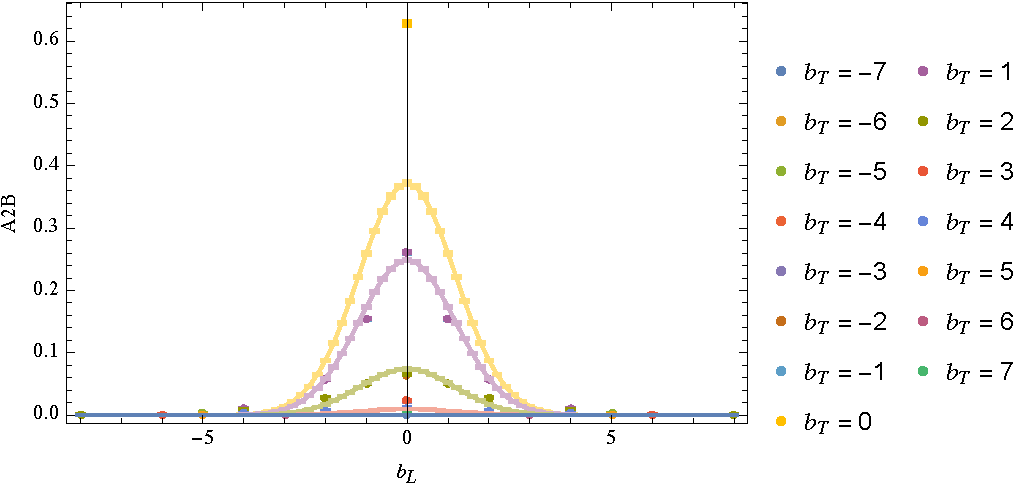
\includegraphics[width=\linewidth,height=.70\textheight,keepaspectratio]{fitting/Gaussian_A2B_Re_P1_FailedFit.pdf}

\figsrc{Thesis: plots; Gaussian\_A2B\_Re\_P1\_FailedFit}
\end{frame}

\begin{frame}{Gaussian parameters and statistics: $\tAmp_{2B}^{\mathrm{Re}}$}
\centering
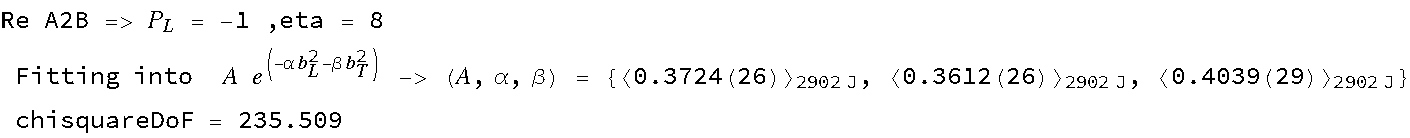
\includegraphics[width=\linewidth]{fitting/Gaussian_A2B_Re_P1_FailedFit_details1.pdf}\\[5mm]
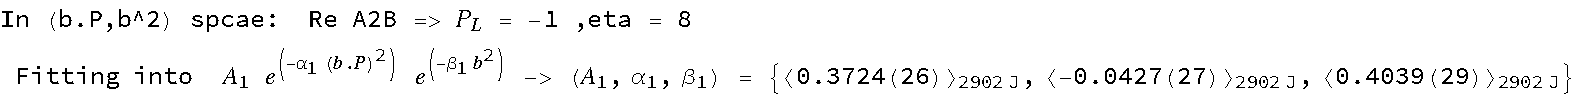
\includegraphics[width=\linewidth]{fitting/Gaussian_A2B_Re_P1_FailedFit_details2.pdf}\\[5mm]

\figsrc{Thesis: Fitting Methodologies and Stability Analysis}
\end{frame}

\begin{frame}{Gaussian fit: $\tAmp_{12B}^{\mathrm{Re}}$}
\centering
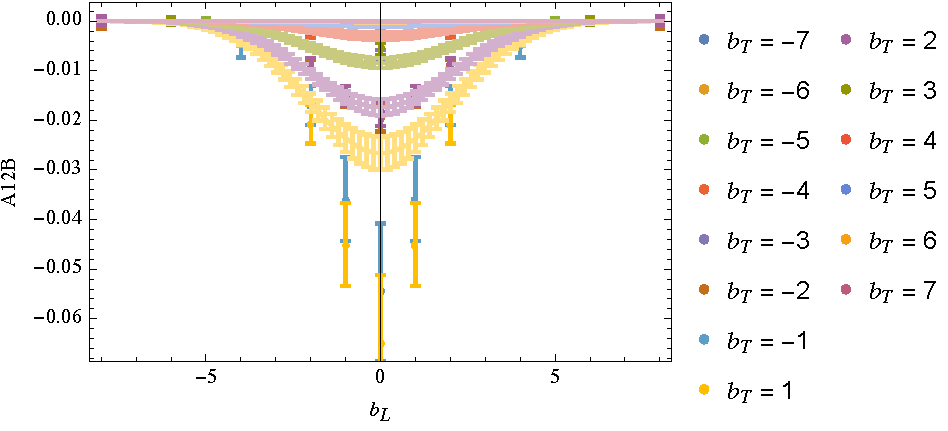
\includegraphics[width=\linewidth,height=.70\textheight,keepaspectratio]{fitting/Gaussian_A12B_Re_P1_FailedFit.pdf}

\figsrc{Thesis: plots; Gaussian\_A12B\_Re\_P1\_FailedFit}
\end{frame}

\begin{frame}{Gaussian parameters and statistics: $\tAmp_{12B}^{\mathrm{Re}}$}
\centering
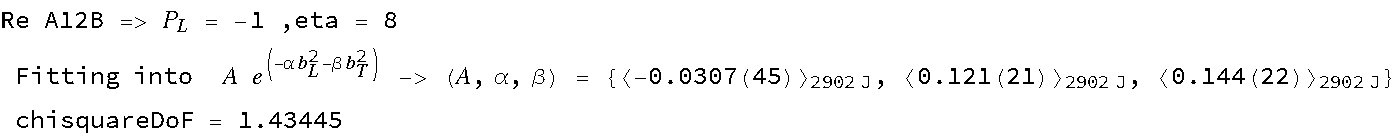
\includegraphics[width=\linewidth]{fitting/Gaussian_A12B_Re_P1_FailedFit_details1.pdf}\\[5mm]
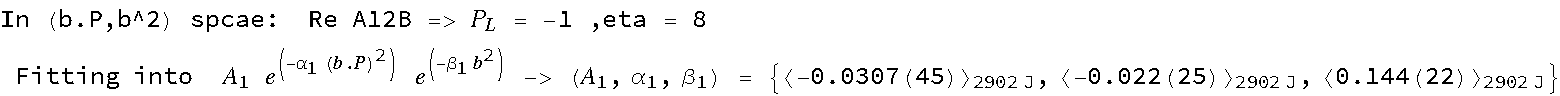
\includegraphics[width=\linewidth]{fitting/Gaussian_A12B_Re_P1_FailedFit_details2.pdf}\\[5mm]

\figsrc{Thesis: Fitting Methodologies and Stability Analysis}
\end{frame}

\begin{frame}{Short-distance diagnostic and the spatial cut}
\centering
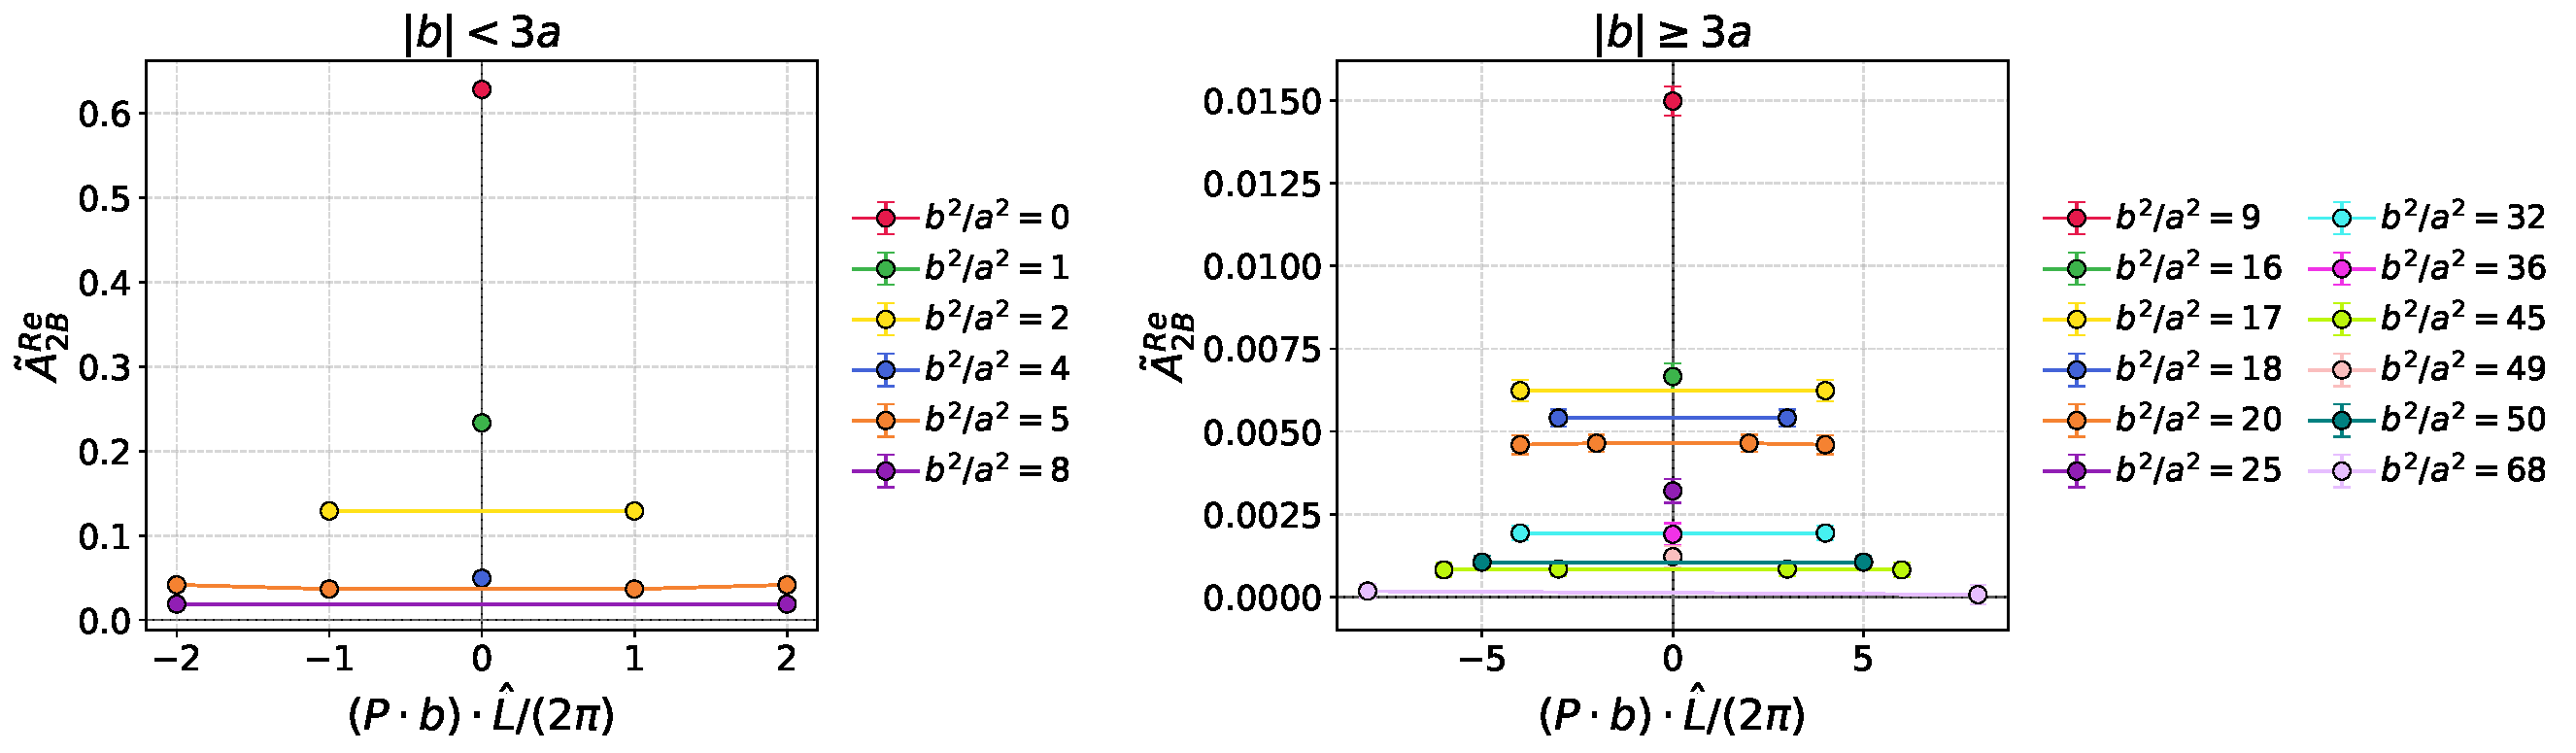
\includegraphics[width=\linewidth,height=.70\textheight,keepaspectratio]{fitting/A2B_Re_b_lessthan3_and_ge3.pdf}
\par\small At $P_L=-1$, $\eta|v|/a=9$, the $b^2/a^2=5$ group rises by about $14\%$. Retain $|\vect b|\ge3a$ in all subsequent fits; this reduces short-distance contamination but does not remove all finite-$a$ effects.

\figsrc{Thesis: plots; A2B\_Re\_b\_lessthan3\_and\_ge3}
\end{frame}

\begin{frame}{Global fit domain and staple dependence}

\[|\vect b|=\sqrt{b_L^2+b_T^2}\ge3a,\qquad6\le\eta|v|/a\le10.\]
\begin{itemize}
\item Fit the full $(b_L,b_T,\eta)$ grid at each fixed nucleon momentum.
\item A common $e^{-f\eta}$ factor is imposed in the final three-amplitude model and cancels in the Sivers ratio.
\item Residual $\eta$ dependence of the real unpolarized width is retained before taking $\eta\to\infty$.
\item The continuation to arbitrary $\nu$ at fixed $b^2$ extends beyond the measured spatial domain $\nu^2\le P_L^2 b^2$; its functional form is a model assumption.
\end{itemize}
\figsrc{Thesis: Fitting Methodologies and Stability Analysis}
\end{frame}

\begin{frame}{PySR: complete search configuration}

\small\renewcommand{\arraystretch}{1.35}
\begin{tabular}{ll}\toprule
Inputs & $\eta,b_L,b_T$; target $\tAmp_{2B}^{\mathrm{Re}}$, $P_L=-1$\\
Binary operators & $+,-,\times,/,\ \operatorname{pow}(u,v)=u^v$\\
Custom binary operator & $\operatorname{lor}(u,v)=(1+u^2+v^2)^{-2}$\\
Unary operators & $u^2,\ \exp(u),\ \operatorname{decay}(u)=e^{-u}$\\
Operator constraints & $\operatorname{pow}:(-1,1)$; $\operatorname{lor}:(10,10)$; decay: $10$\\
Forbidden nesting & exp inside exp; decay inside decay; decay inside exp\\
Populations / iterations & $30\,/\,100$\\
Maximum tree complexity & $28$\\
Regularization weight & $\epsilon=0.1$\\\bottomrule
\end{tabular}
\par\medskip The search explores expression trees; operator choices favor some families over others.
\figsrc{Thesis: PySR configuration; target momentum corrected to match chapter and plots}
\end{frame}

\begin{frame}{PySR loss: the implemented objective}

\[\mathcal L=\frac{1}{N_{\rm data}-3}\sum_{i=1}^{N_{\rm data}}
\frac{[F(\eta_i,b_{L,i},b_{T,i})-y_i]^2}{\sigma_i^2}
+0.1\sum_{p\in\mathcal P}F(p)^2.\]
\[\mathcal P=\{(10,50,1),(10,80,1),(10,10,1),(8,20,1),(6,30,2)\},\]
where each tuple is $(\eta,b_L/a,b_T/a)$.
\begin{itemize}
\item Invalid data predictions return infinite loss; an invalid penalty prediction adds $10^6$ before multiplication by $0.1$.
\item These finite probes discourage large predictions; they do not prove convergence of an infinite Fourier integral.
\item The source code uses squared predictions and a fixed $N_{\rm data}-3$ normalization. Reported loss is therefore not a model-by-model reduced $\chi^2$.
\end{itemize}
\figsrc{Thesis: exact objective in PySR outputs / custom loss Julia listing}
\end{frame}

\begin{frame}{PySR Pareto front: stored candidates (1/7)}
\small $B=1+b_L^2+b_T^2$, $L(u,v)=(1+u^2+v^2)^{-2}$.\par\medskip\renewcommand{\arraystretch}{2.0}\begin{tabular}{ccl}\toprule $C$ & Loss & Exact stored expression\\\midrule
1 & 276.43433 & $0.005040839$ \\
3 & 171.56175 & $0.49875718^\eta$ \\
4 & 167.5698 & $e^{-\eta^{0.80833286}}$ \\
5 & 130.85486 & $34.16954\,L(\eta,b_L)$ \\\bottomrule\end{tabular}
\figsrc{Source: PySR outputs\_A2B\_real / 20260821\_101855\_eCTY5z / hall\_of\_fame.csv}
\end{frame}

\begin{frame}{PySR Pareto front: stored candidates (2/7)}
\small $B=1+b_L^2+b_T^2$, $L(u,v)=(1+u^2+v^2)^{-2}$.\par\medskip\renewcommand{\arraystretch}{2.0}\begin{tabular}{ccl}\toprule $C$ & Loss & Exact stored expression\\\midrule
7 & 68.93352 & $(11.584338-\eta)B^{-2}$ \\
9 & 30.807978 & $(10.156917-\eta)B^{-1.7775426}$ \\
11 & 5.158913 & $(7.0522256/\eta)^4 B^{-1.44250464}$ \\
12 & 4.7633114 & $[(\eta-14.485626)/\eta]^2 B^{-1.4604364}$ \\\bottomrule\end{tabular}
\figsrc{Source: PySR outputs\_A2B\_real / 20260821\_101855\_eCTY5z / hall\_of\_fame.csv}
\end{frame}

\begin{frame}{PySR Pareto front: stored candidates (3/7)}
\small $B=1+b_L^2+b_T^2$, $L(u,v)=(1+u^2+v^2)^{-2}$.\par\medskip\renewcommand{\arraystretch}{2.0}\begin{tabular}{ccl}\toprule $C$ & Loss & Exact stored expression\\\midrule
14 & 3.934378 & $\frac{e^{-0.534084(\eta-8.68932)}}{2.6322825\,B^{1.390951}}$ \\
16 & 2.0260298 & $\frac{e^{-0.46820307(\eta-8.994358)}}{3.5930288\,B^{1.2585272}}-0.0012706916$ \\\bottomrule\end{tabular}
\figsrc{Source: PySR outputs\_A2B\_real / 20260821\_101855\_eCTY5z / hall\_of\_fame.csv}
\end{frame}

\begin{frame}{PySR Pareto front: stored candidates (4/7)}
\small $B=1+b_L^2+b_T^2$, $L(u,v)=(1+u^2+v^2)^{-2}$.\par\medskip\renewcommand{\arraystretch}{2.0}\begin{tabular}{ccl}\toprule $C$ & Loss & Exact stored expression\\\midrule
17 & 1.9917132 & $\left(\frac{10.461691}{\eta}\right)^{2.3353815}\frac{B^{-1.2146622}}{0.593981\eta}-0.0016621732$ \\
18 & 1.9095322 & $\frac{B^{-1.251997}}{1.4630643}\left(\frac{17.983559-\eta}{-1.560787\eta}\right)^2-0.0013669281$ \\\bottomrule\end{tabular}
\figsrc{Source: PySR outputs\_A2B\_real / 20260821\_101855\_eCTY5z / hall\_of\_fame.csv}
\end{frame}

\begin{frame}{PySR Pareto front: stored candidates (5/7)}
\small $B=1+b_L^2+b_T^2$, $L(u,v)=(1+u^2+v^2)^{-2}$.\par\medskip\renewcommand{\arraystretch}{2.0}\begin{tabular}{ccl}\toprule $C$ & Loss & Exact stored expression\\\midrule
19 & 1.7628223 & $\frac1\eta\left(\frac{10.381556}{\eta}\right)^{2.369394}\left(\frac{B^{-1.1273306}}{0.7187267}-0.0032199204\right)-0.0014922422$ \\
21 & 1.7604288 & $\frac1\eta\left(\frac{10.300505}{\eta}\right)^{2.4254909}\left(\frac{B^{-1.1335096}}{0.71366495}-0.003188983\right)-0.001388529$ \\\bottomrule\end{tabular}
\figsrc{Source: PySR outputs\_A2B\_real / 20260821\_101855\_eCTY5z / hall\_of\_fame.csv}
\end{frame}

\begin{frame}{PySR Pareto front: stored candidates (6/7)}
\small $L(u,v)=(1+u^2+v^2)^{-2}$; these higher-complexity stored candidates were omitted from the thesis table.\par
\[\Delta_{22}=b_L-L(-0.1626809,b_L^2),\qquad\mathcal L_{22}=1.6167384.\]
\[F_{22}=\frac{L(\Delta_{22},b_T)^{0.66107386}}{\eta}\left(\frac{14.42762}{\eta+0.12903585}\right)^{2.5097084}-0.0012624399.\]
\[\Delta_{23}=b_L-L(b_L,0.213843),\qquad\mathcal L_{23}=1.5782435.\]
\[F_{23}=\frac{2.7467434\,L(b_T,\Delta_{23})^{0.6493724}}{\eta}\left(\frac{10.018184}{\eta+0.7164768}\right)^{2.6639583}-0.0013878929.\]
These shifted spatial profiles are not even in $b_L$; they require a symmetry check before physical use.
\figsrc{Source: PySR outputs\_A2B\_real / 20260821\_101855\_eCTY5z / hall\_of\_fame.csv}
\end{frame}

\begin{frame}{PySR Pareto front: stored candidates (7/7)}
\small $L(u,v)=(1+u^2+v^2)^{-2}$; these higher-complexity stored candidates were omitted from the thesis table.\par
\[\Delta_{25}=b_L-L(b_L,0.04371186\eta),\qquad\mathcal L_{25}=1.5110264.\]
\[F_{25}=\frac{2.7467434\,L(\Delta_{25},b_T)^{0.6493724}}{\eta}\left(\frac{10.018184}{\eta+0.7164768}\right)^{2.6639583}-0.0013878929.\]
\[\Delta_{27}=b_L-L(2b_L,0.04371186\eta),\qquad\mathcal L_{27}=1.5023776.\]
\[F_{27}=\frac{2.7467434\,L(b_T,\Delta_{27})^{0.6493724}}{\eta}\left(\frac{10.018184}{\eta+0.7164768}\right)^{2.6639583}-0.0013878929.\]
These shifted spatial profiles are not even in $b_L$; they require a symmetry check before physical use.
\figsrc{Source: PySR outputs\_A2B\_real / 20260821\_101855\_eCTY5z / hall\_of\_fame.csv}
\end{frame}

\begin{frame}{PySR benchmark models: panels 1 and 2}
\centering
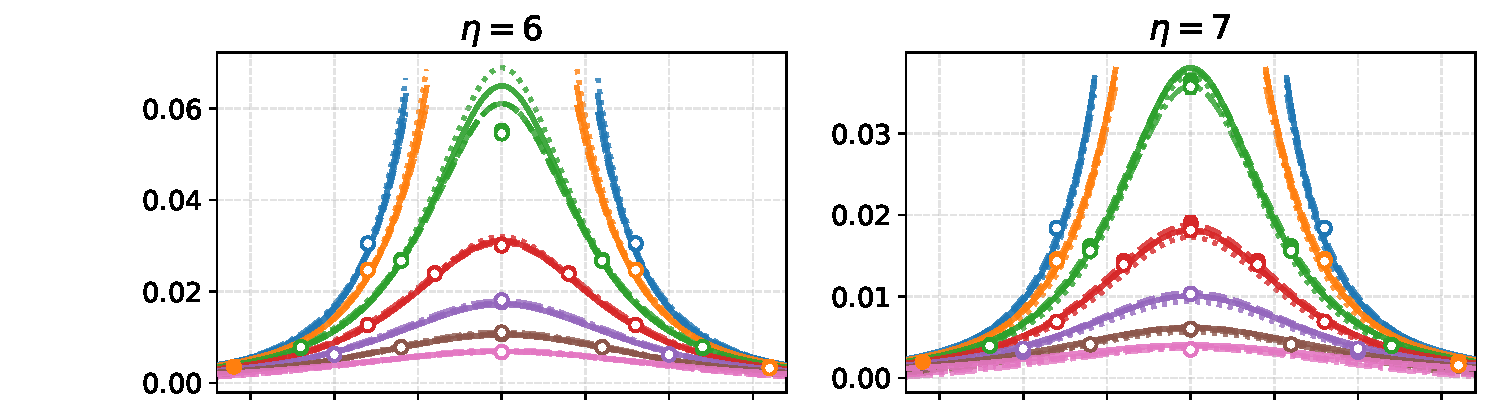
\includegraphics[width=\linewidth,height=.70\textheight,keepaspectratio]{fitting/01_A2B_PySR_Benchmark_Fits__row1.pdf}
\par\small All four overlays: $C=11,14,16,17$; curves restricted to $|\vect b|\ge3a$.

\figsrc{Thesis: PySR\_outputs; 01\_A2B\_PySR\_Benchmark\_Fits}
\end{frame}

\begin{frame}{PySR benchmark models: panels 3 and 4}
\centering
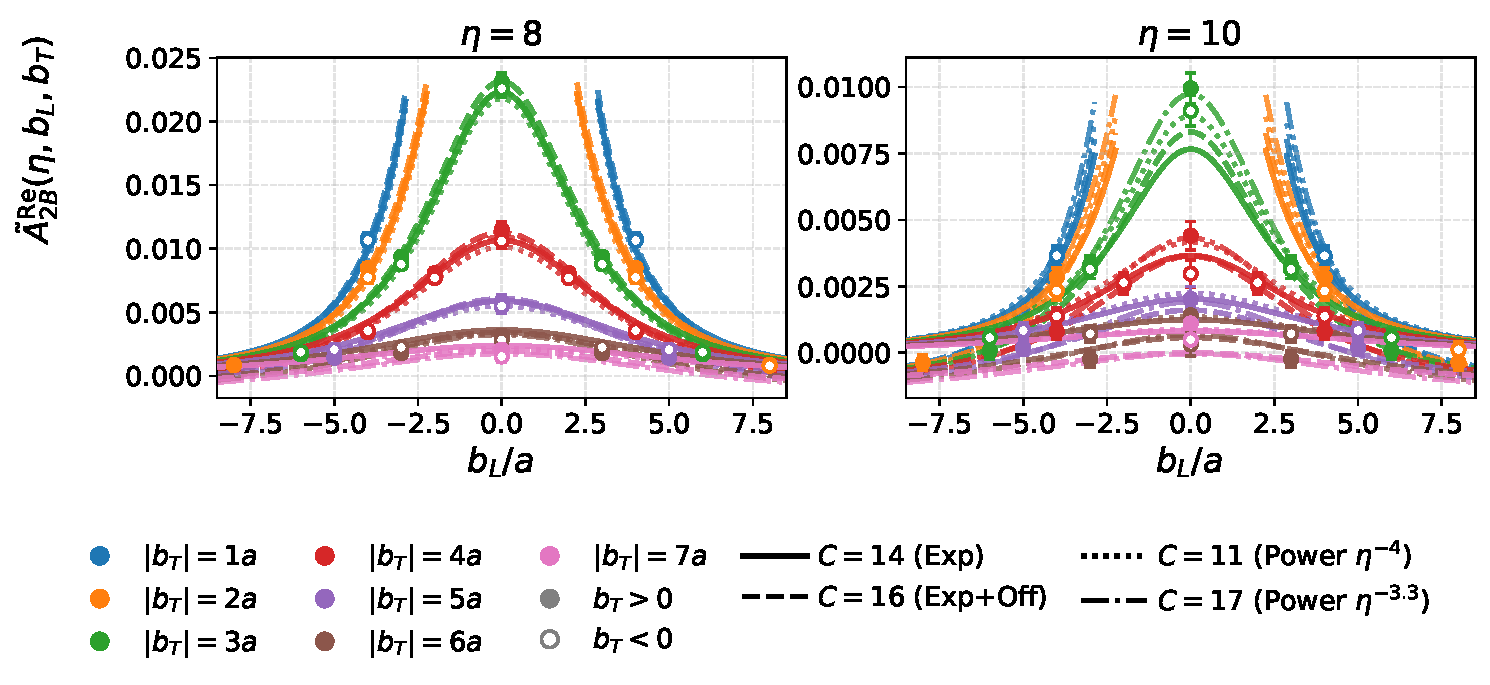
\includegraphics[width=\linewidth,height=.70\textheight,keepaspectratio]{fitting/01_A2B_PySR_Benchmark_Fits__row2.pdf}
\par\small All four overlays: $C=11,14,16,17$; curves restricted to $|\vect b|\ge3a$.

\figsrc{Thesis: PySR\_outputs; 01\_A2B\_PySR\_Benchmark\_Fits}
\end{frame}

\begin{frame}{Gaussian straight-line diagnostic}
\centering
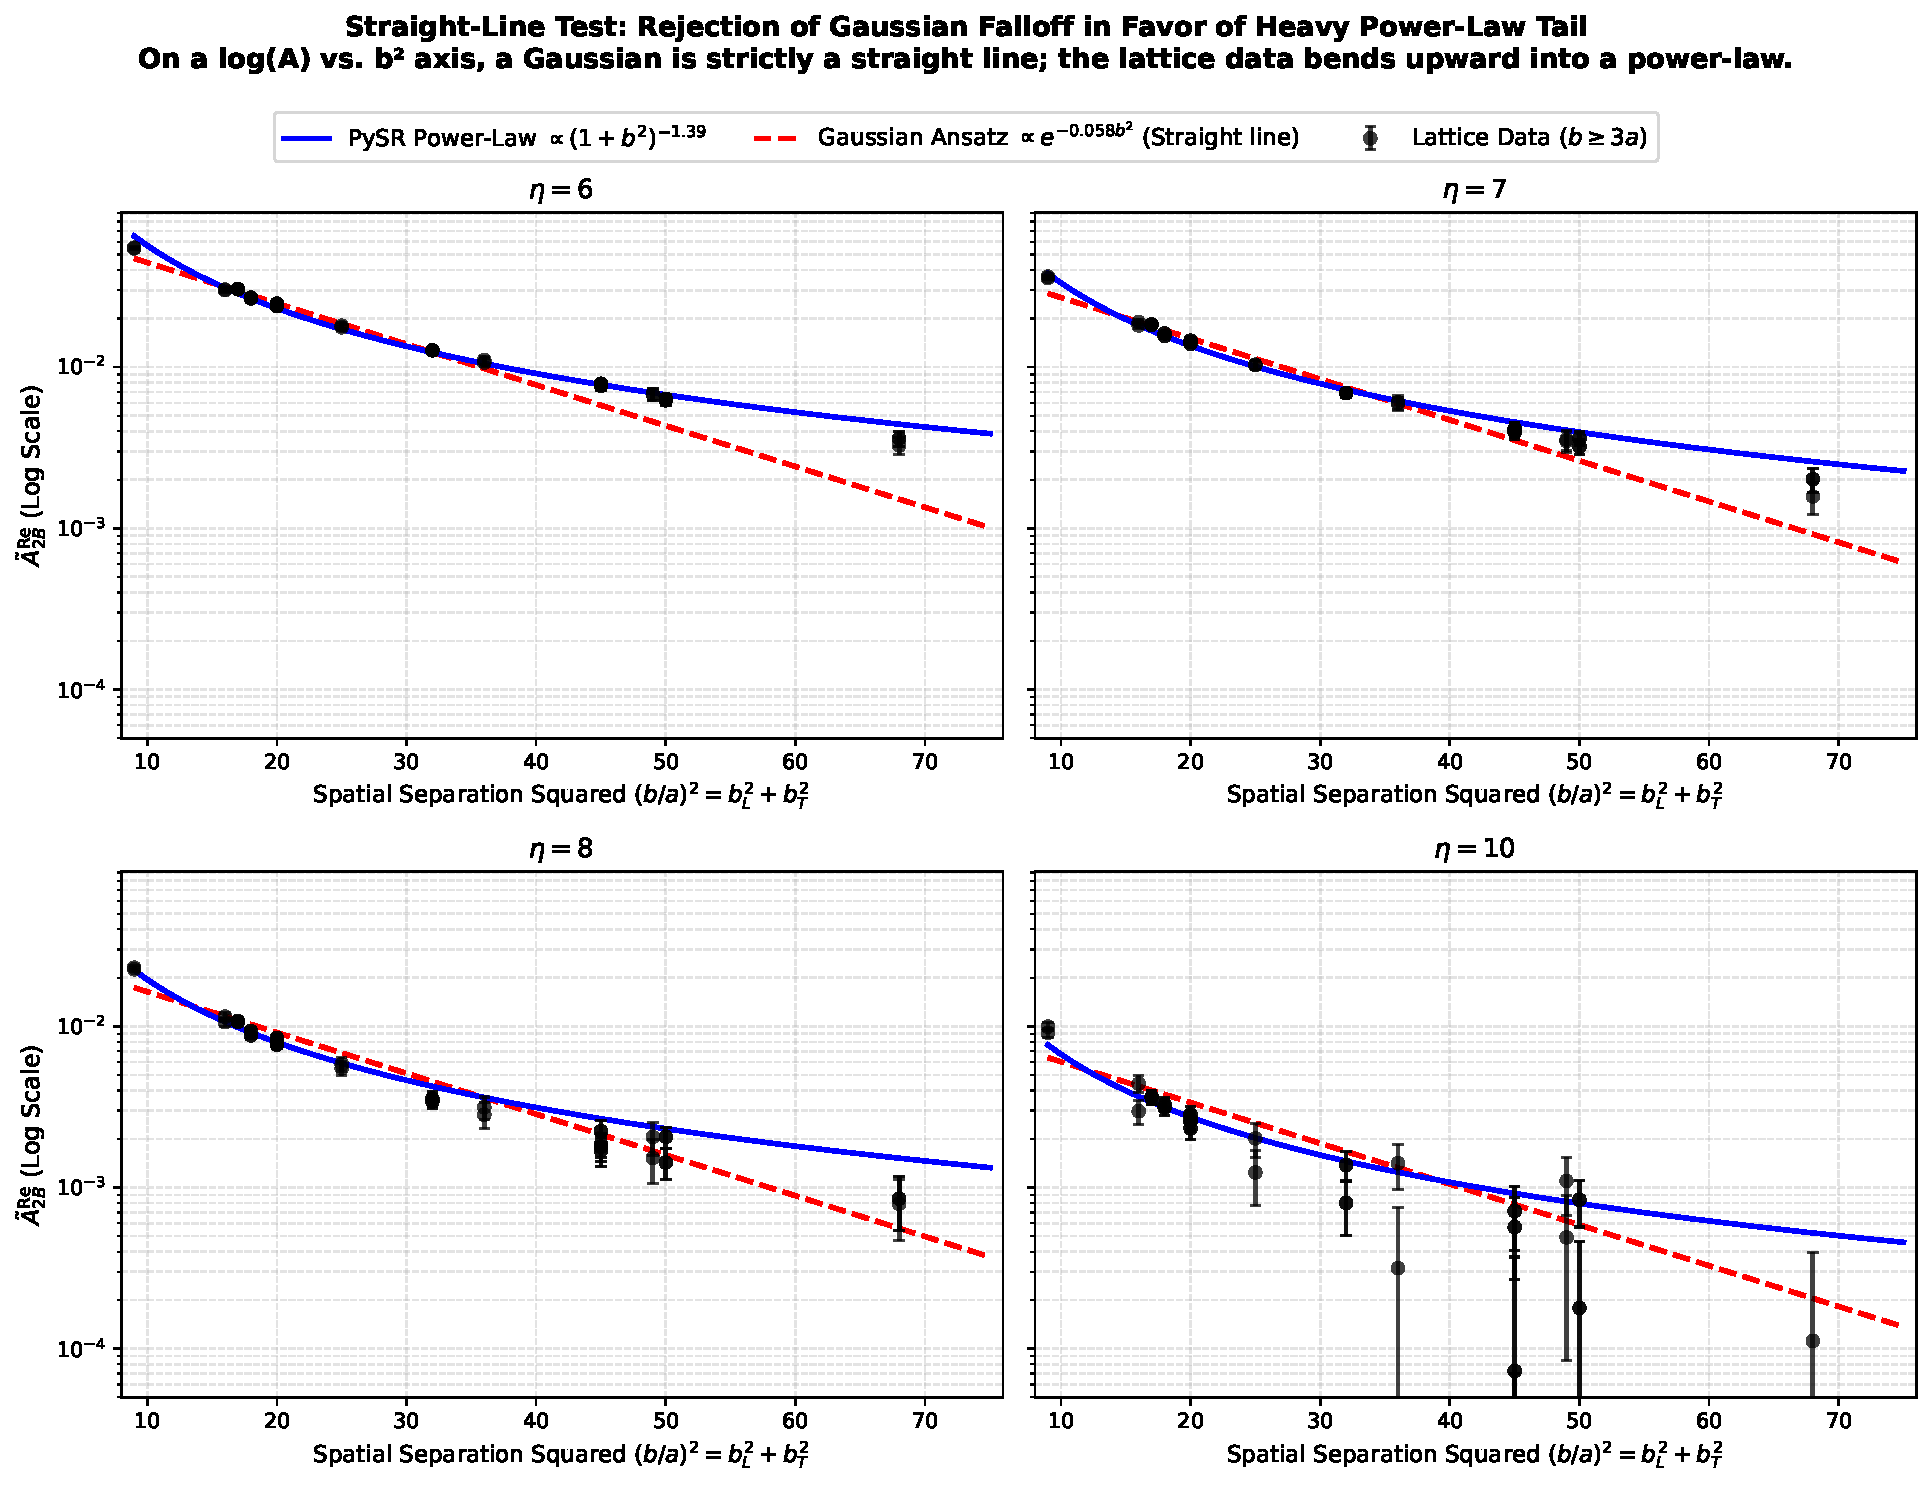
\includegraphics[width=\linewidth,height=.70\textheight,keepaspectratio]{fitting/02_Gaussian_StraightLine_Test.pdf}
\par\small $\log\tAmp_{2B}^{\mathrm{Re}}$ versus $b^2$: the data bend away from the Gaussian baseline ($c=0.058$).

\figsrc{Thesis: PySR\_outputs; 02\_Gaussian\_StraightLine\_Test}
\end{frame}

\begin{frame}{What symbolic regression establishes}

\[F_{14}=\frac{39.36887e^{-0.534084\eta}}{(1+b^2)^{1.390951}},\qquad
F_{16}=\frac{18.76870e^{-0.46820307\eta}}{(1+b^2)^{1.2585272}}-0.0012706916.\]
\begin{itemize}
\item A power-law spatial envelope and an exponential staple profile describe the retained finite grid.
\item At fixed $b^2$, the thesis-highlighted $C=14,16$ expressions have no $\nu=P\cdot b$ dependence. They are guides to the final model, not directly usable ordinary Fourier-integrable longitudinal profiles.
\item Nonzero offsets also survive at large spatial separation; the finite-probe loss does not enforce exact decay to zero.
\item Exact stored formulas correct the thesis prefactors ($39.71$, $245.5$) and the $C=21$ grouping. Higher-complexity stored candidates also need an even-parity check.\item No square-root operator was provided: $e^{-c|\vect b|}$ is more costly for this search to construct.
\end{itemize}
\figsrc{Thesis: Fitting Methodologies and Stability Analysis}
\end{frame}

\begin{frame}{Exponential spatial decay remains competitive}
\centering
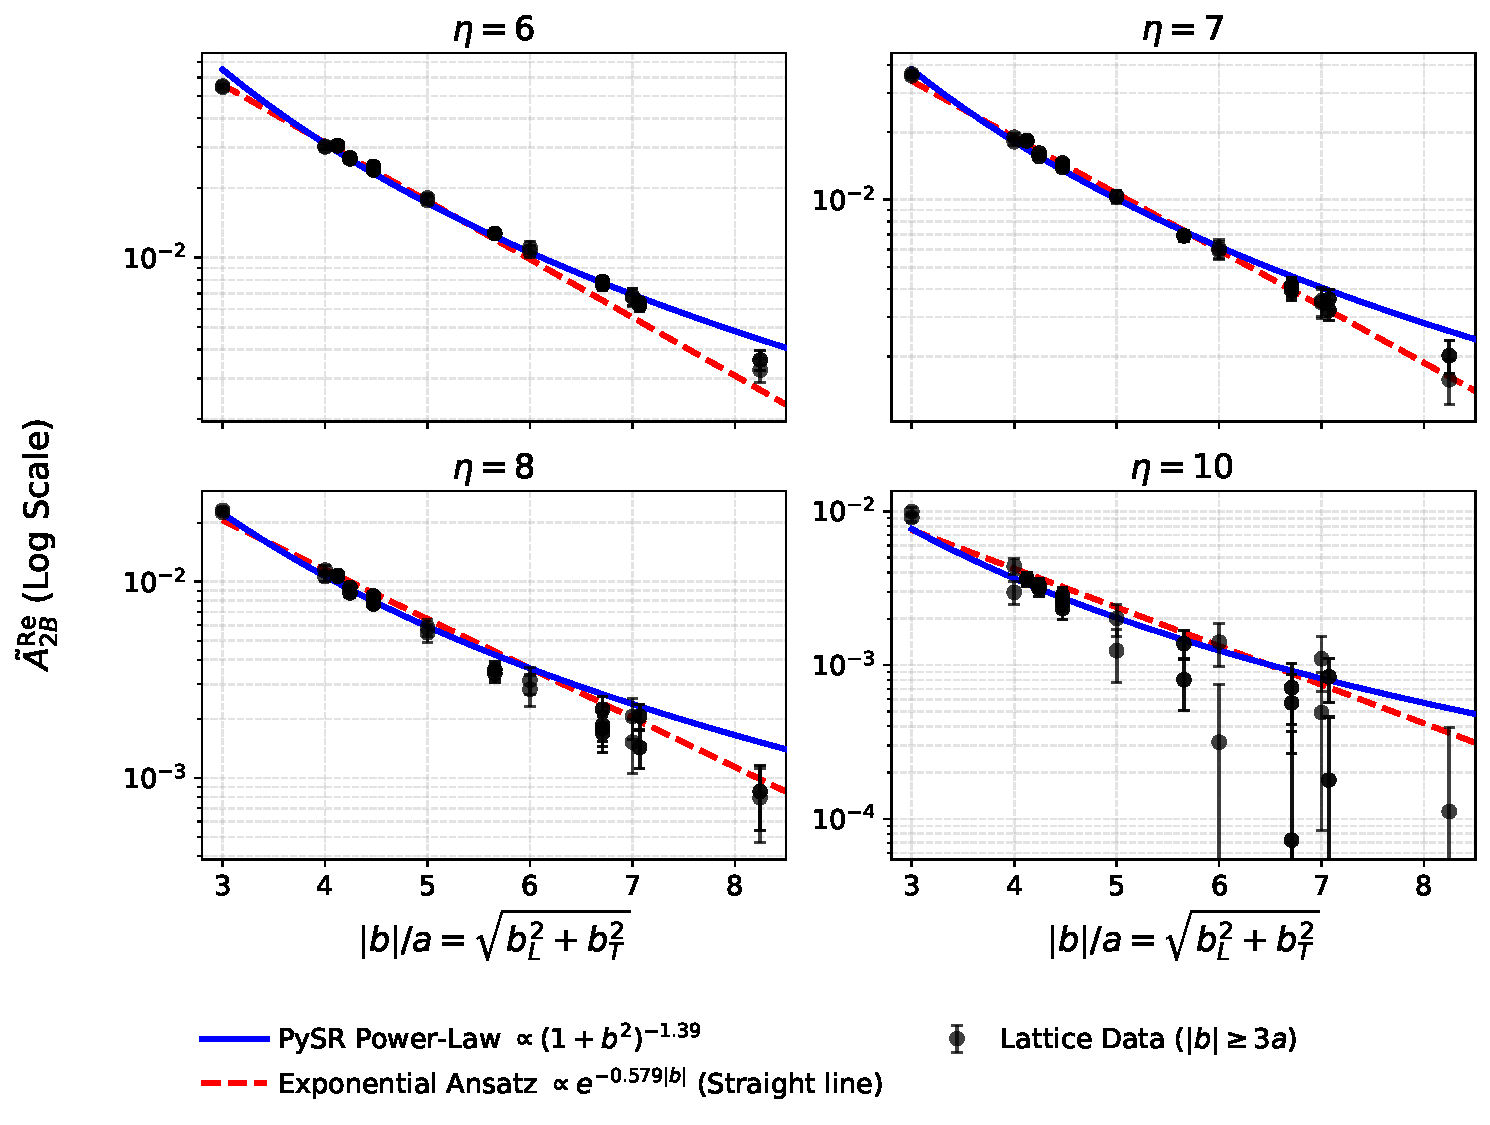
\includegraphics[width=\linewidth,height=.70\textheight,keepaspectratio]{fitting/03_Exponential_b_StraightLine_Test.pdf}
\par\small $e^{-c|\vect b|}$ with $c=0.579$ describes the real unpolarized data over $3\le|\vect b|/a\le8.2$. Direct losses: about $2.63$, or $2.26$ with an offset.

\figsrc{Thesis: PySR\_outputs; 03\_Exponential\_b\_StraightLine\_Test}
\end{frame}

\begin{frame}{Separable real-unpolarized candidates: constant width --- models}
\centering
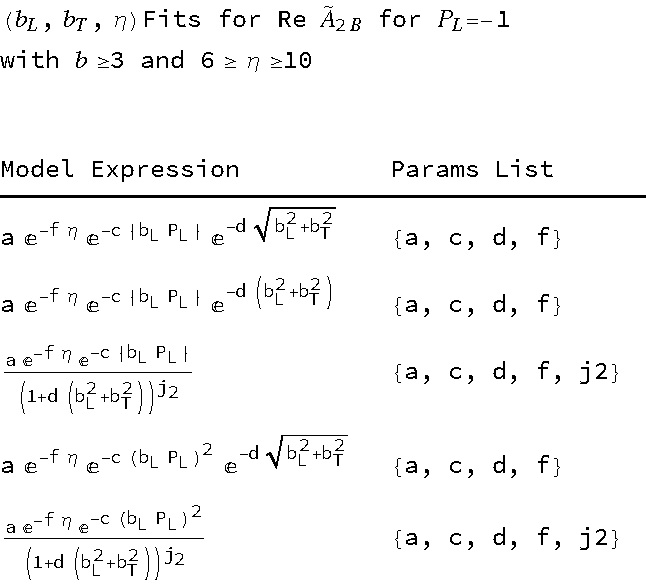
\includegraphics[width=\linewidth,height=.70\textheight,keepaspectratio]{fitting/Rejection-of-Separable-Exponential-Longitudinal-Decay__part1.pdf}
\par\small Five tested forms; all parameter values and $\chi^2/\mathrm{dof}$ retained. Correct cut: $6\le\eta\le10$.

\figsrc{Thesis: plots; Rejection-of-Separable-Exponential-Longitudinal-Decay}
\end{frame}

\begin{frame}{Separable real-unpolarized candidates: constant width --- fit results}
\centering
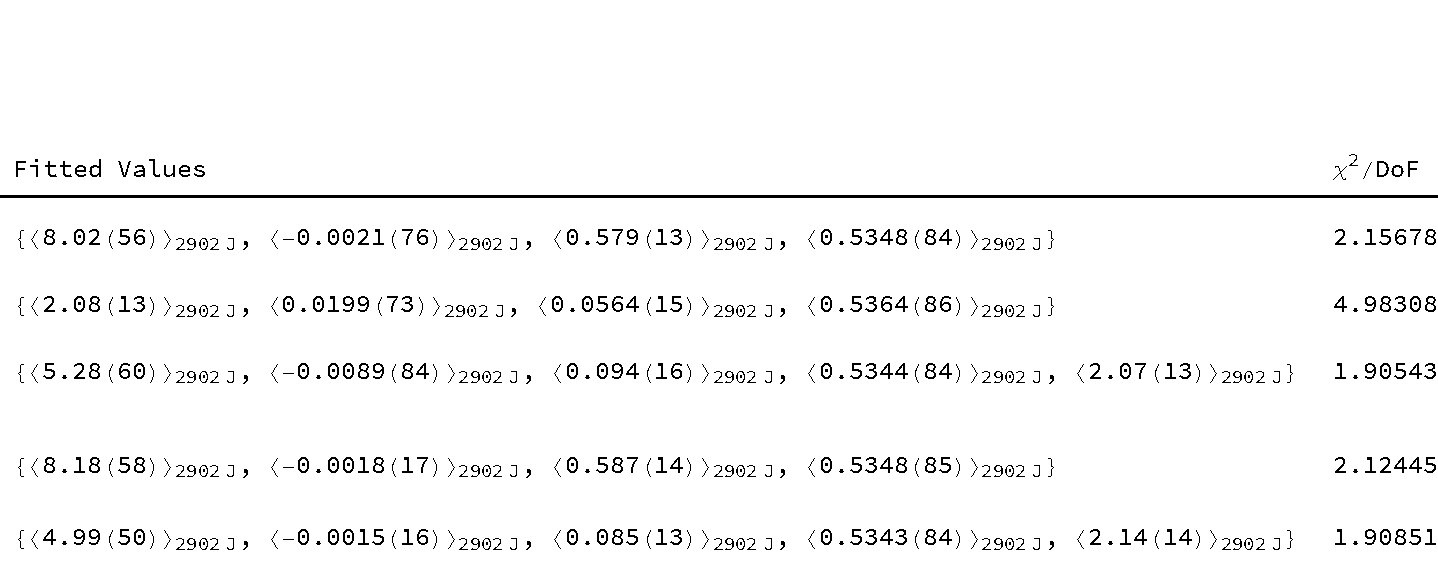
\includegraphics[width=\linewidth,height=.70\textheight,keepaspectratio]{fitting/Rejection-of-Separable-Exponential-Longitudinal-Decay__part2.pdf}
\par\small Five tested forms; all parameter values and $\chi^2/\mathrm{dof}$ retained. Correct cut: $6\le\eta\le10$.

\figsrc{Thesis: plots; Rejection-of-Separable-Exponential-Longitudinal-Decay}
\end{frame}

\begin{frame}{Separable real-unpolarized candidates: variable width --- models}
\centering
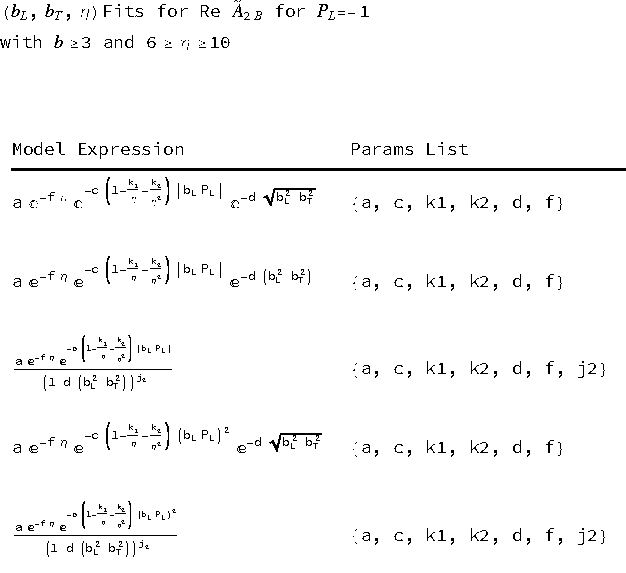
\includegraphics[width=\linewidth,height=.70\textheight,keepaspectratio]{fitting/Rejection-of-Separable-Exponential-Longitudinal-Decay-ceta__part1.pdf}
\par\small Five tested forms; all parameter values and $\chi^2/\mathrm{dof}$ retained. Correct cut: $6\le\eta\le10$.

\figsrc{Thesis: plots; Rejection-of-Separable-Exponential-Longitudinal-Decay-ceta}
\end{frame}

\begin{frame}{Separable real-unpolarized candidates: variable width --- fit results}
\centering
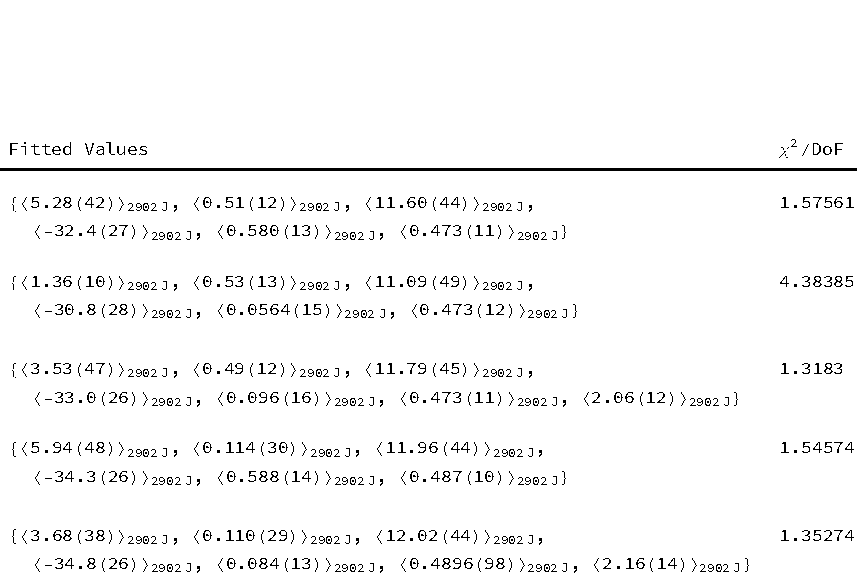
\includegraphics[width=\linewidth,height=.70\textheight,keepaspectratio]{fitting/Rejection-of-Separable-Exponential-Longitudinal-Decay-ceta__part2.pdf}
\par\small Five tested forms; all parameter values and $\chi^2/\mathrm{dof}$ retained. Correct cut: $6\le\eta\le10$.

\figsrc{Thesis: plots; Rejection-of-Separable-Exponential-Longitudinal-Decay-ceta}
\end{frame}

\begin{frame}{Sixteen Gaussian candidates: the full family}

\[F_{rs}=a e^{-f\eta}\exp[-c\,g_r(\eta;k_1,k_2)\nu^2-d\,g_s(\eta;l_1,l_2)b^2],\]
\[\begin{aligned}
g_0(\eta;u,v)&=1,&g_1(\eta;u,v)&=1-\frac{u}{\eta},\\
g_2(\eta;u,v)&=1+\frac{u}{\eta}-\frac{v}{\sqrt\eta},&
g_3(\eta;u,v)&=1-\frac{u}{\eta}-\frac{v}{\eta^2}.
\end{aligned}\]
\[\begin{array}{c|cccc}
 &g_0(d)&g_1(d)&g_2(d)&g_3(d)\\\hline
 g_0(c)&1&5&6&7\\g_1(c)&2&8&9&10\\g_2(c)&3&11&12&13\\g_3(c)&4&14&15&16
\end{array}\]
Numbers identify the original table rows. The next slides retain every expression, parameter estimate, and fit statistic.
\figsrc{Thesis: Fitting Methodologies and Stability Analysis}
\end{frame}

\begin{frame}{Gaussian candidates --- block 1, models}
\centering
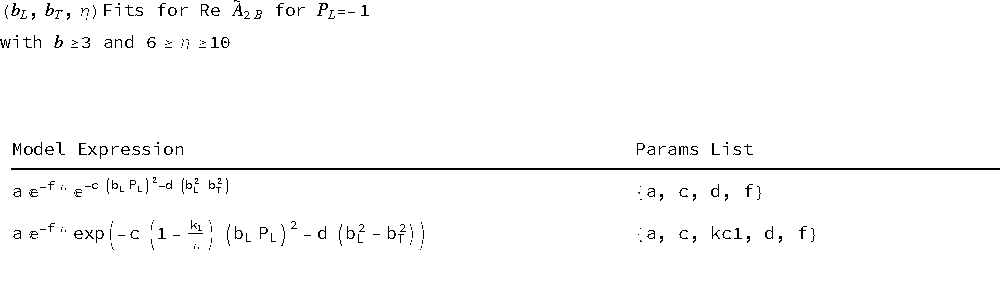
\includegraphics[width=\linewidth,height=.72\textheight,keepaspectratio]{fitting/fit_list_gaussian_c_d_etas__block1_part1.pdf}
\par\small $P_L=-1$, $|\vect b|\ge3a$, $6\le\eta\le10$. Original thesis table, enlarged without omitted rows.

\figsrc{Thesis: plots; fit\_list\_gaussian\_c\_d\_etas}
\end{frame}

\begin{frame}{Gaussian candidates --- block 1, parameters and diagnostics}
\centering
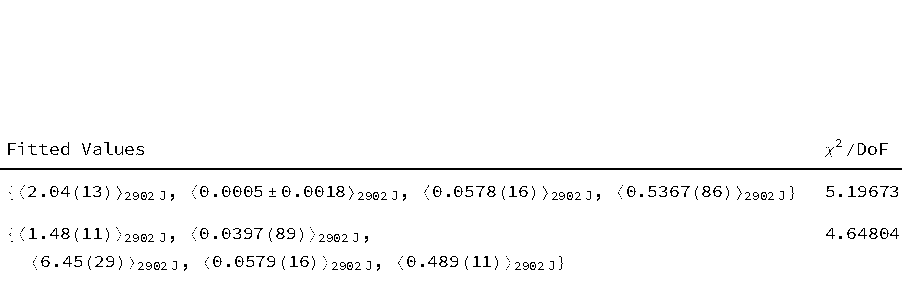
\includegraphics[width=\linewidth,height=.72\textheight,keepaspectratio]{fitting/fit_list_gaussian_c_d_etas__block1_part2.pdf}
\par\small $P_L=-1$, $|\vect b|\ge3a$, $6\le\eta\le10$. Original thesis table, enlarged without omitted rows.

\figsrc{Thesis: plots; fit\_list\_gaussian\_c\_d\_etas}
\end{frame}

\begin{frame}{Gaussian candidates --- block 2, models}
\centering
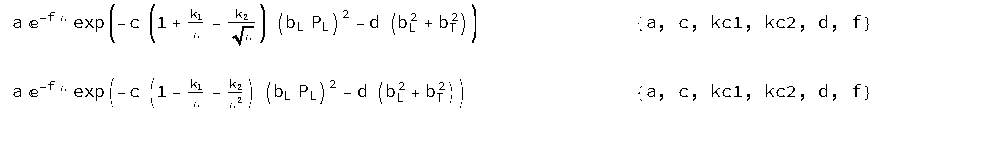
\includegraphics[width=\linewidth,height=.72\textheight,keepaspectratio]{fitting/fit_list_gaussian_c_d_etas__block2_part1.pdf}
\par\small $P_L=-1$, $|\vect b|\ge3a$, $6\le\eta\le10$. Original thesis table, enlarged without omitted rows.

\figsrc{Thesis: plots; fit\_list\_gaussian\_c\_d\_etas}
\end{frame}

\begin{frame}{Gaussian candidates --- block 2, parameters and diagnostics}
\centering
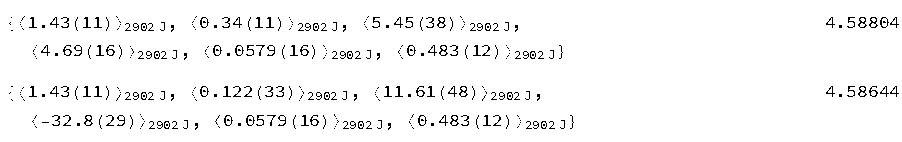
\includegraphics[width=\linewidth,height=.72\textheight,keepaspectratio]{fitting/fit_list_gaussian_c_d_etas__block2_part2.pdf}
\par\small $P_L=-1$, $|\vect b|\ge3a$, $6\le\eta\le10$. Original thesis table, enlarged without omitted rows.

\figsrc{Thesis: plots; fit\_list\_gaussian\_c\_d\_etas}
\end{frame}

\begin{frame}{Gaussian candidates --- block 3, models}
\centering
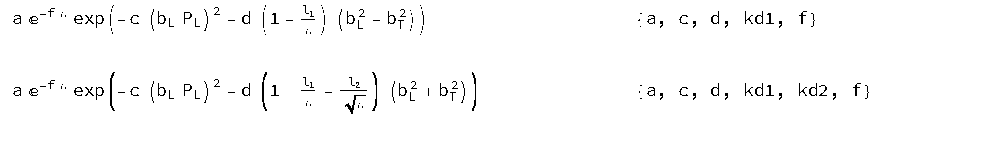
\includegraphics[width=\linewidth,height=.72\textheight,keepaspectratio]{fitting/fit_list_gaussian_c_d_etas__block3_part1.pdf}
\par\small $P_L=-1$, $|\vect b|\ge3a$, $6\le\eta\le10$. Original thesis table, enlarged without omitted rows.

\figsrc{Thesis: plots; fit\_list\_gaussian\_c\_d\_etas}
\end{frame}

\begin{frame}{Gaussian candidates --- block 3, parameters and diagnostics}
\centering
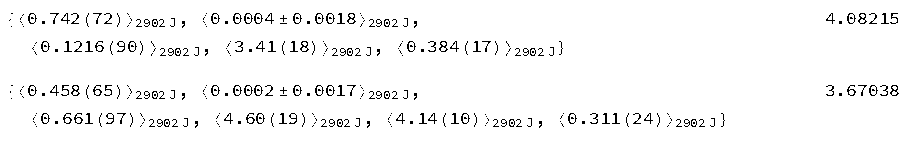
\includegraphics[width=\linewidth,height=.72\textheight,keepaspectratio]{fitting/fit_list_gaussian_c_d_etas__block3_part2.pdf}
\par\small $P_L=-1$, $|\vect b|\ge3a$, $6\le\eta\le10$. Original thesis table, enlarged without omitted rows.

\figsrc{Thesis: plots; fit\_list\_gaussian\_c\_d\_etas}
\end{frame}

\begin{frame}{Gaussian candidates --- block 4, models}
\centering
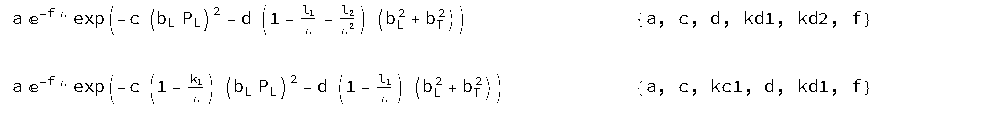
\includegraphics[width=\linewidth,height=.72\textheight,keepaspectratio]{fitting/fit_list_gaussian_c_d_etas__block4_part1.pdf}
\par\small $P_L=-1$, $|\vect b|\ge3a$, $6\le\eta\le10$. Original thesis table, enlarged without omitted rows.

\figsrc{Thesis: plots; fit\_list\_gaussian\_c\_d\_etas}
\end{frame}

\begin{frame}{Gaussian candidates --- block 4, parameters and diagnostics}
\centering
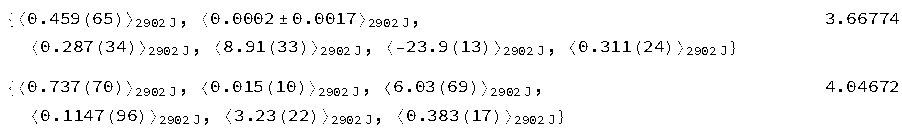
\includegraphics[width=\linewidth,height=.72\textheight,keepaspectratio]{fitting/fit_list_gaussian_c_d_etas__block4_part2.pdf}
\par\small $P_L=-1$, $|\vect b|\ge3a$, $6\le\eta\le10$. Original thesis table, enlarged without omitted rows.

\figsrc{Thesis: plots; fit\_list\_gaussian\_c\_d\_etas}
\end{frame}

\begin{frame}{Gaussian candidates --- block 5, models}
\centering
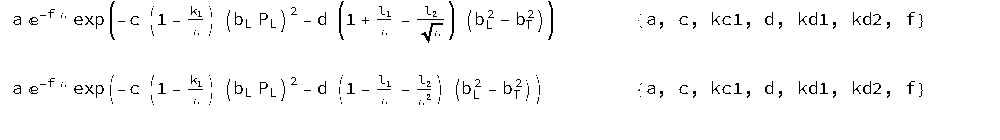
\includegraphics[width=\linewidth,height=.72\textheight,keepaspectratio]{fitting/fit_list_gaussian_c_d_etas__block5_part1.pdf}
\par\small $P_L=-1$, $|\vect b|\ge3a$, $6\le\eta\le10$. Original thesis table, enlarged without omitted rows.

\figsrc{Thesis: plots; fit\_list\_gaussian\_c\_d\_etas}
\end{frame}

\begin{frame}{Gaussian candidates --- block 5, parameters and diagnostics}
\centering
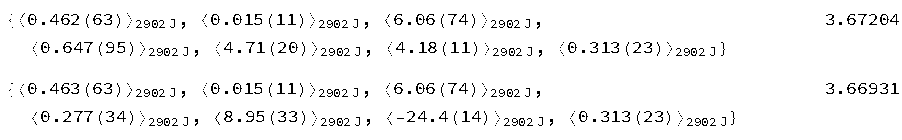
\includegraphics[width=\linewidth,height=.72\textheight,keepaspectratio]{fitting/fit_list_gaussian_c_d_etas__block5_part2.pdf}
\par\small $P_L=-1$, $|\vect b|\ge3a$, $6\le\eta\le10$. Original thesis table, enlarged without omitted rows.

\figsrc{Thesis: plots; fit\_list\_gaussian\_c\_d\_etas}
\end{frame}

\begin{frame}{Gaussian candidates --- block 6, models}
\centering
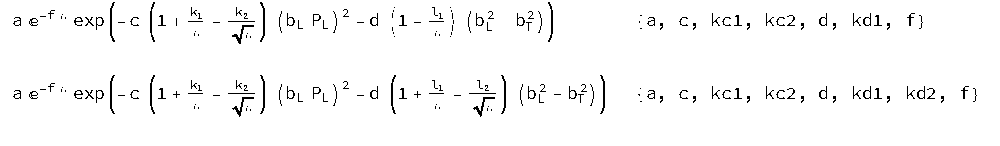
\includegraphics[width=\linewidth,height=.72\textheight,keepaspectratio]{fitting/fit_list_gaussian_c_d_etas__block6_part1.pdf}
\par\small $P_L=-1$, $|\vect b|\ge3a$, $6\le\eta\le10$. Original thesis table, enlarged without omitted rows.

\figsrc{Thesis: plots; fit\_list\_gaussian\_c\_d\_etas}
\end{frame}

\begin{frame}{Gaussian candidates --- block 6, parameters and diagnostics}
\centering
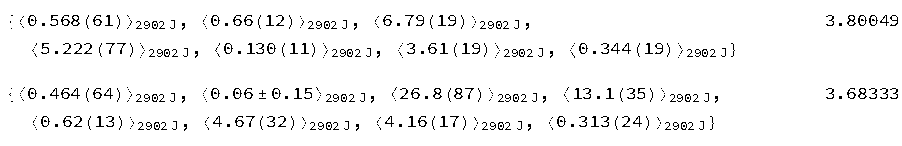
\includegraphics[width=\linewidth,height=.72\textheight,keepaspectratio]{fitting/fit_list_gaussian_c_d_etas__block6_part2.pdf}
\par\small $P_L=-1$, $|\vect b|\ge3a$, $6\le\eta\le10$. Original thesis table, enlarged without omitted rows.

\figsrc{Thesis: plots; fit\_list\_gaussian\_c\_d\_etas}
\end{frame}

\begin{frame}{Gaussian candidates --- block 7, models}
\centering
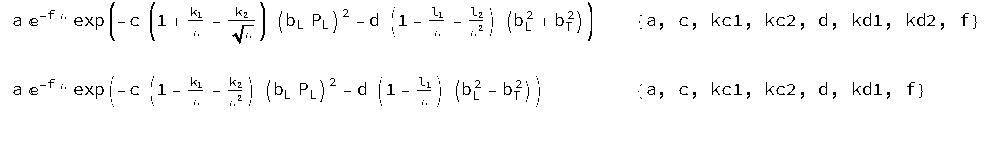
\includegraphics[width=\linewidth,height=.72\textheight,keepaspectratio]{fitting/fit_list_gaussian_c_d_etas__block7_part1.pdf}
\par\small $P_L=-1$, $|\vect b|\ge3a$, $6\le\eta\le10$. Original thesis table, enlarged without omitted rows.

\figsrc{Thesis: plots; fit\_list\_gaussian\_c\_d\_etas}
\end{frame}

\begin{frame}{Gaussian candidates --- block 7, parameters and diagnostics}
\centering
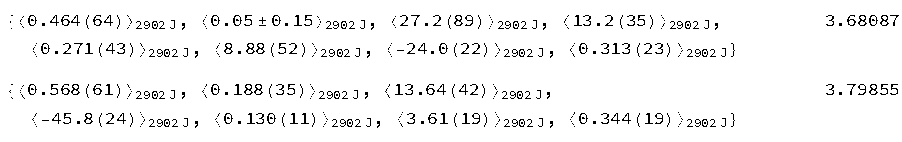
\includegraphics[width=\linewidth,height=.72\textheight,keepaspectratio]{fitting/fit_list_gaussian_c_d_etas__block7_part2.pdf}
\par\small $P_L=-1$, $|\vect b|\ge3a$, $6\le\eta\le10$. Original thesis table, enlarged without omitted rows.

\figsrc{Thesis: plots; fit\_list\_gaussian\_c\_d\_etas}
\end{frame}

\begin{frame}{Gaussian candidates --- block 8, models}
\centering
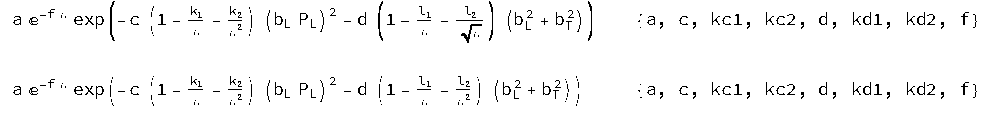
\includegraphics[width=\linewidth,height=.72\textheight,keepaspectratio]{fitting/fit_list_gaussian_c_d_etas__block8_part1.pdf}
\par\small $P_L=-1$, $|\vect b|\ge3a$, $6\le\eta\le10$. Original thesis table, enlarged without omitted rows.

\figsrc{Thesis: plots; fit\_list\_gaussian\_c\_d\_etas}
\end{frame}

\begin{frame}{Gaussian candidates --- block 8, parameters and diagnostics}
\centering
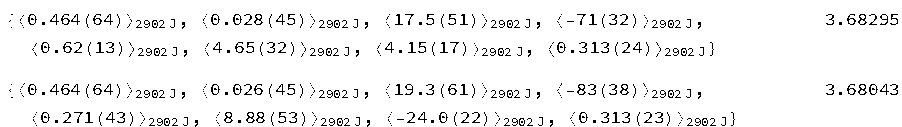
\includegraphics[width=\linewidth,height=.72\textheight,keepaspectratio]{fitting/fit_list_gaussian_c_d_etas__block8_part2.pdf}
\par\small $P_L=-1$, $|\vect b|\ge3a$, $6\le\eta\le10$. Original thesis table, enlarged without omitted rows.

\figsrc{Thesis: plots; fit\_list\_gaussian\_c\_d\_etas}
\end{frame}

\begin{frame}{Power-law candidates: finite-width continuation}

\[F(\nu,b^2,\eta)=a e^{-f\eta}\left[1+c(\eta)\frac{\nu^2}{P_L^2}+db^2\right]^{-j}.\]
\begin{itemize}
\item First compare a constant $c$, inverse powers of $\eta$, logarithmic corrections, and an exponential correction.
\item Then compare forms giving wider Fourier profiles. Each original row includes its full equation, parameters, $\chi^2/\mathrm{dof}$, AIC, and Fourier plot.
\item AIC compares likelihood fit quality and parameter count on the same data: $\mathrm{AIC}=2k-2\log\widehat{\mathcal L}$; for fixed Gaussian covariance this is $\chi^2+2k$ up to a common constant.
\end{itemize}
\figsrc{Thesis: Fitting Methodologies and Stability Analysis}
\end{frame}

\begin{frame}{Power-law candidate diagnostics --- block 1, models}
\centering
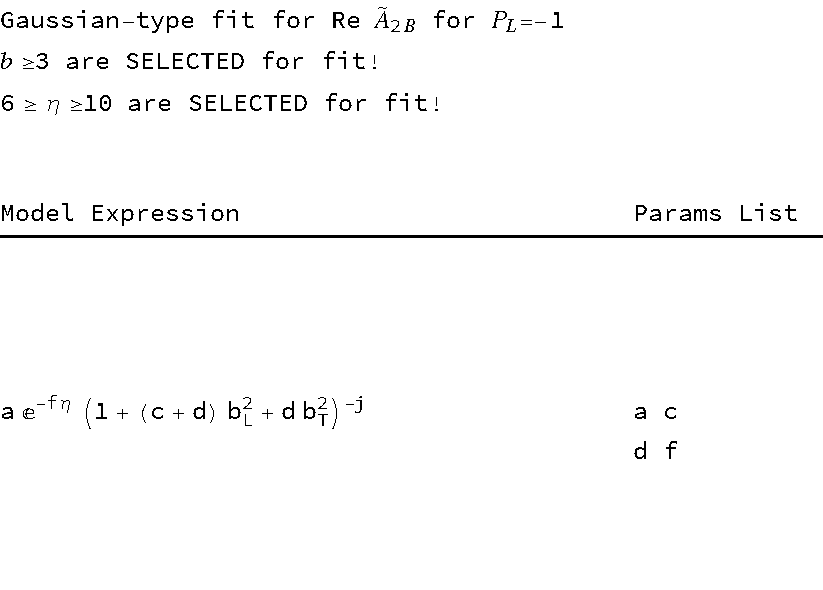
\includegraphics[width=\linewidth,height=.72\textheight,keepaspectratio]{fitting/A2BfitFT_eta_Asymptotic_P1__block1_part1.pdf}
\par\small $P_L=-1$, $|\vect b|\ge3a$, $6\le\eta\le10$. Original thesis table, enlarged without omitted rows.

\figsrc{Thesis: PowerLaw\_etaAsymptotic; A2BfitFT\_eta\_Asymptotic\_P1}
\end{frame}

\begin{frame}{Power-law candidate diagnostics --- block 1, parameters and diagnostics}
\centering
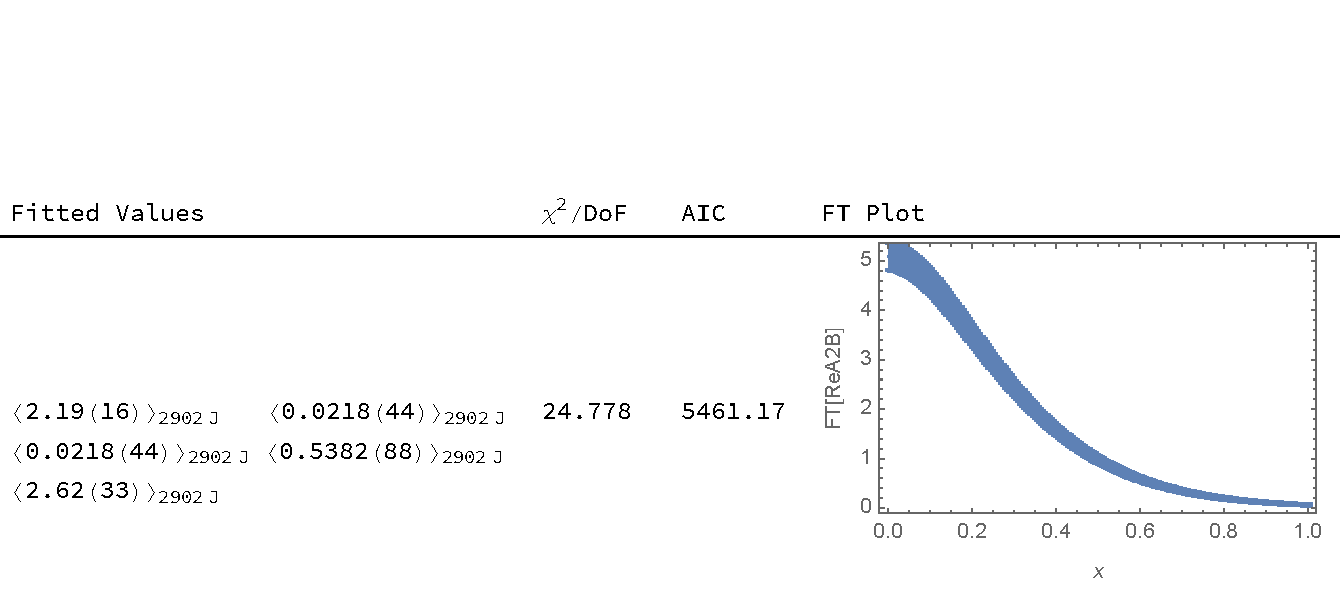
\includegraphics[width=\linewidth,height=.72\textheight,keepaspectratio]{fitting/A2BfitFT_eta_Asymptotic_P1__block1_part2.pdf}
\par\small $P_L=-1$, $|\vect b|\ge3a$, $6\le\eta\le10$. Original thesis table, enlarged without omitted rows.

\figsrc{Thesis: PowerLaw\_etaAsymptotic; A2BfitFT\_eta\_Asymptotic\_P1}
\end{frame}

\begin{frame}{Power-law candidate diagnostics --- block 2, models}
\centering
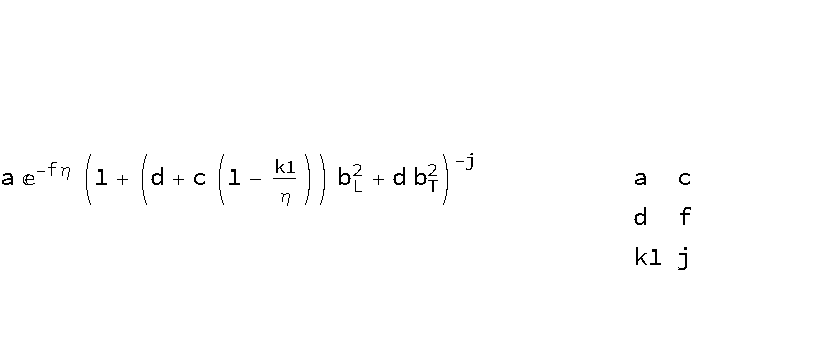
\includegraphics[width=\linewidth,height=.72\textheight,keepaspectratio]{fitting/A2BfitFT_eta_Asymptotic_P1__block2_part1.pdf}
\par\small $P_L=-1$, $|\vect b|\ge3a$, $6\le\eta\le10$. Original thesis table, enlarged without omitted rows.

\figsrc{Thesis: PowerLaw\_etaAsymptotic; A2BfitFT\_eta\_Asymptotic\_P1}
\end{frame}

\begin{frame}{Power-law candidate diagnostics --- block 2, parameters and diagnostics}
\centering
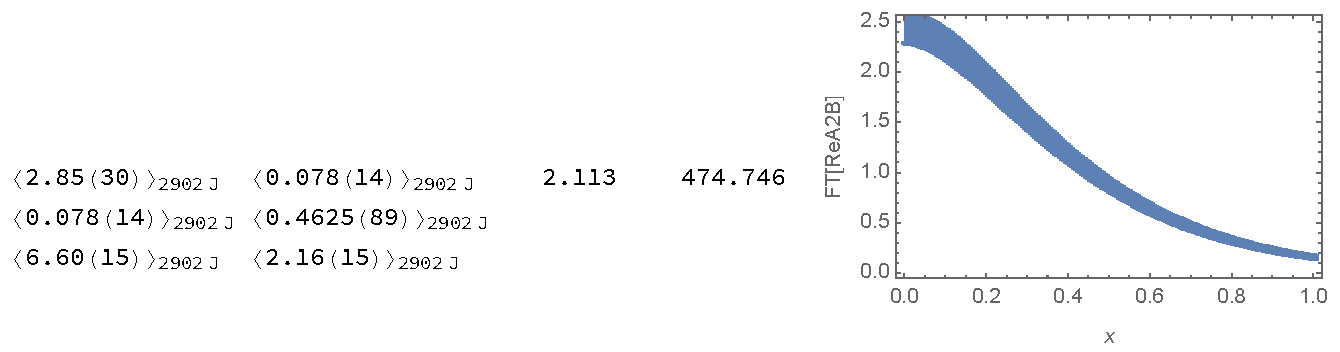
\includegraphics[width=\linewidth,height=.72\textheight,keepaspectratio]{fitting/A2BfitFT_eta_Asymptotic_P1__block2_part2.pdf}
\par\small $P_L=-1$, $|\vect b|\ge3a$, $6\le\eta\le10$. Original thesis table, enlarged without omitted rows.

\figsrc{Thesis: PowerLaw\_etaAsymptotic; A2BfitFT\_eta\_Asymptotic\_P1}
\end{frame}

\begin{frame}{Power-law candidate diagnostics --- block 3, models}
\centering
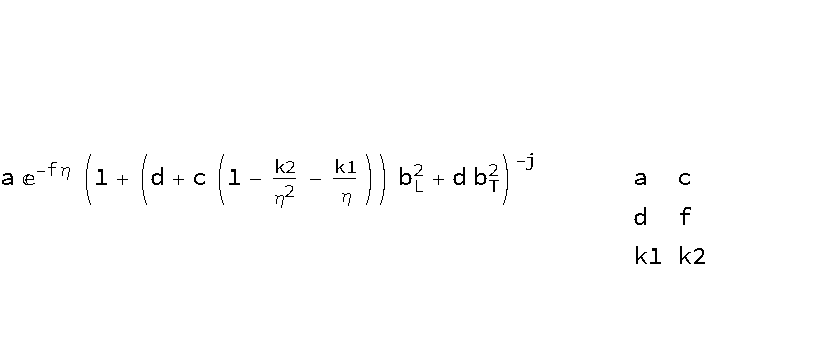
\includegraphics[width=\linewidth,height=.72\textheight,keepaspectratio]{fitting/A2BfitFT_eta_Asymptotic_P1__block3_part1.pdf}
\par\small $P_L=-1$, $|\vect b|\ge3a$, $6\le\eta\le10$. Original thesis table, enlarged without omitted rows.

\figsrc{Thesis: PowerLaw\_etaAsymptotic; A2BfitFT\_eta\_Asymptotic\_P1}
\end{frame}

\begin{frame}{Power-law candidate diagnostics --- block 3, parameters and diagnostics}
\centering
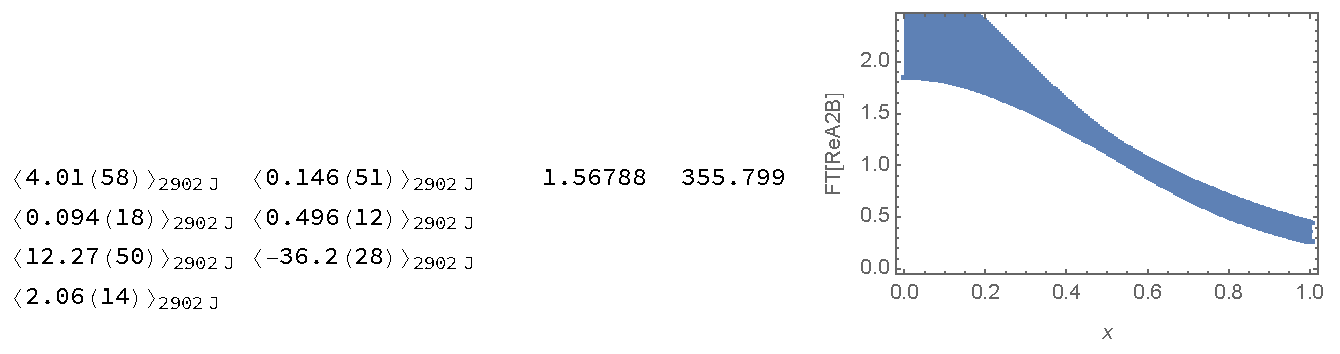
\includegraphics[width=\linewidth,height=.72\textheight,keepaspectratio]{fitting/A2BfitFT_eta_Asymptotic_P1__block3_part2.pdf}
\par\small $P_L=-1$, $|\vect b|\ge3a$, $6\le\eta\le10$. Original thesis table, enlarged without omitted rows.

\figsrc{Thesis: PowerLaw\_etaAsymptotic; A2BfitFT\_eta\_Asymptotic\_P1}
\end{frame}

\begin{frame}{Power-law candidate diagnostics --- block 4, models}
\centering
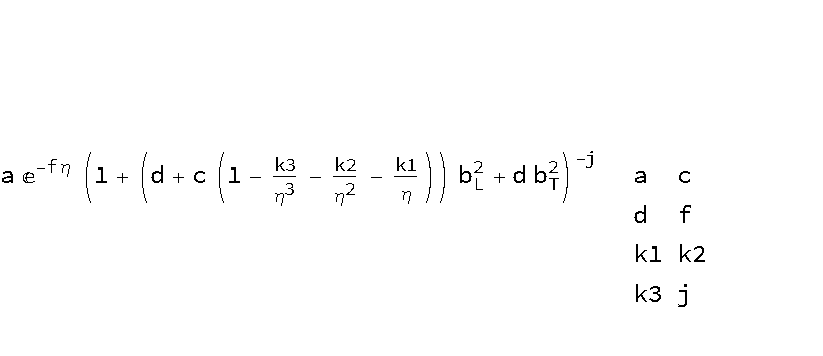
\includegraphics[width=\linewidth,height=.72\textheight,keepaspectratio]{fitting/A2BfitFT_eta_Asymptotic_P1__block4_part1.pdf}
\par\small $P_L=-1$, $|\vect b|\ge3a$, $6\le\eta\le10$. Original thesis table, enlarged without omitted rows.

\figsrc{Thesis: PowerLaw\_etaAsymptotic; A2BfitFT\_eta\_Asymptotic\_P1}
\end{frame}

\begin{frame}{Power-law candidate diagnostics --- block 4, parameters and diagnostics}
\centering
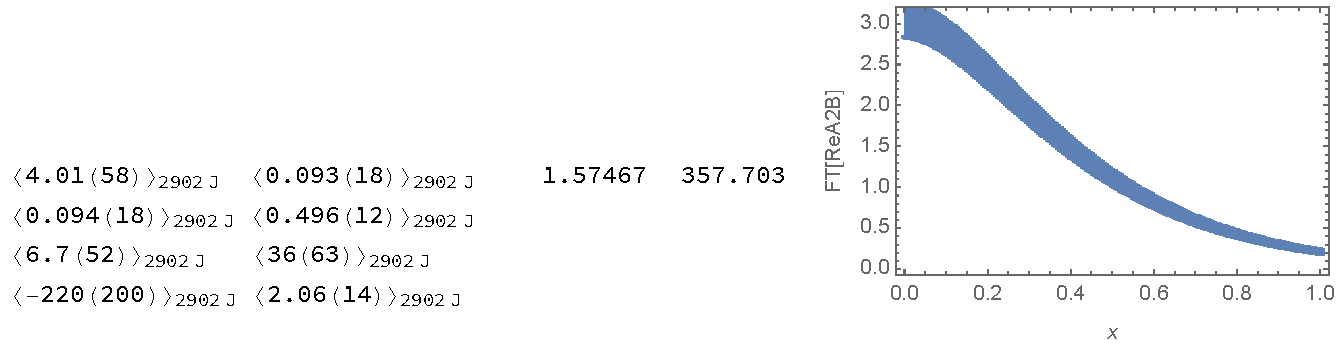
\includegraphics[width=\linewidth,height=.72\textheight,keepaspectratio]{fitting/A2BfitFT_eta_Asymptotic_P1__block4_part2.pdf}
\par\small $P_L=-1$, $|\vect b|\ge3a$, $6\le\eta\le10$. Original thesis table, enlarged without omitted rows.

\figsrc{Thesis: PowerLaw\_etaAsymptotic; A2BfitFT\_eta\_Asymptotic\_P1}
\end{frame}

\begin{frame}{Power-law candidate diagnostics --- block 5, models}
\centering
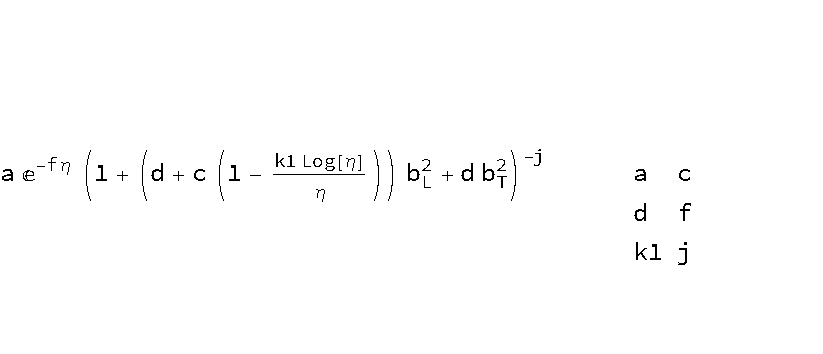
\includegraphics[width=\linewidth,height=.72\textheight,keepaspectratio]{fitting/A2BfitFT_eta_Asymptotic_P1__block5_part1.pdf}
\par\small $P_L=-1$, $|\vect b|\ge3a$, $6\le\eta\le10$. Original thesis table, enlarged without omitted rows.

\figsrc{Thesis: PowerLaw\_etaAsymptotic; A2BfitFT\_eta\_Asymptotic\_P1}
\end{frame}

\begin{frame}{Power-law candidate diagnostics --- block 5, parameters and diagnostics}
\centering
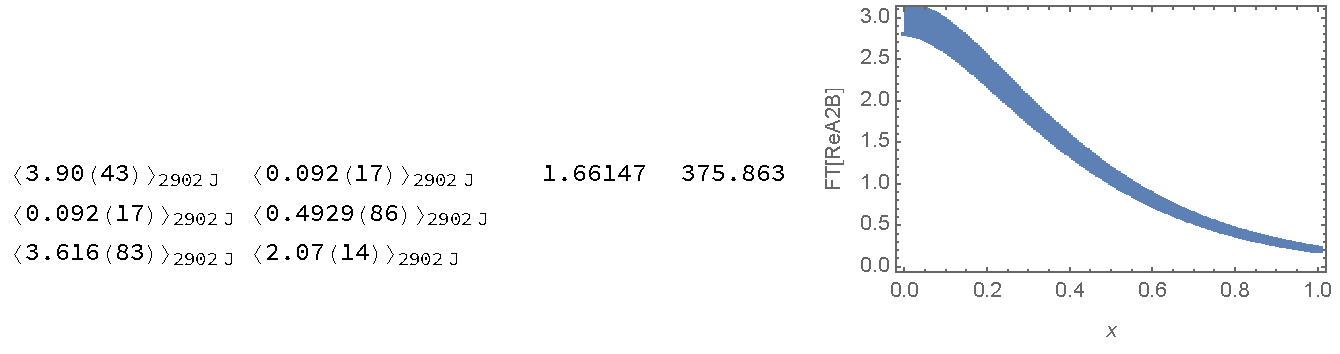
\includegraphics[width=\linewidth,height=.72\textheight,keepaspectratio]{fitting/A2BfitFT_eta_Asymptotic_P1__block5_part2.pdf}
\par\small $P_L=-1$, $|\vect b|\ge3a$, $6\le\eta\le10$. Original thesis table, enlarged without omitted rows.

\figsrc{Thesis: PowerLaw\_etaAsymptotic; A2BfitFT\_eta\_Asymptotic\_P1}
\end{frame}

\begin{frame}{Power-law candidate diagnostics --- block 6, models}
\centering
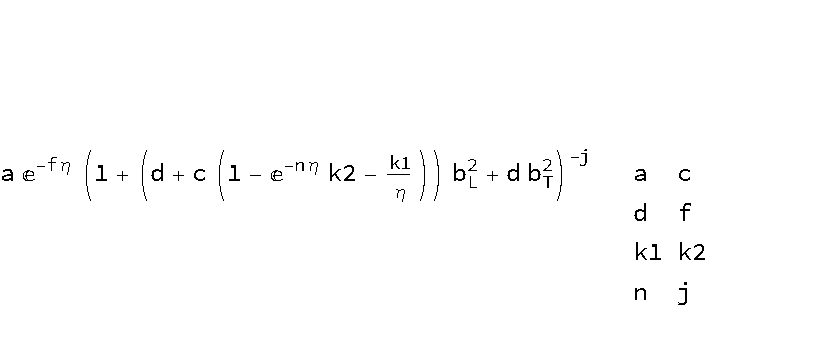
\includegraphics[width=\linewidth,height=.72\textheight,keepaspectratio]{fitting/A2BfitFT_eta_Asymptotic_P1__block6_part1.pdf}
\par\small $P_L=-1$, $|\vect b|\ge3a$, $6\le\eta\le10$. Original thesis table, enlarged without omitted rows.

\figsrc{Thesis: PowerLaw\_etaAsymptotic; A2BfitFT\_eta\_Asymptotic\_P1}
\end{frame}

\begin{frame}{Power-law candidate diagnostics --- block 6, parameters and diagnostics}
\centering
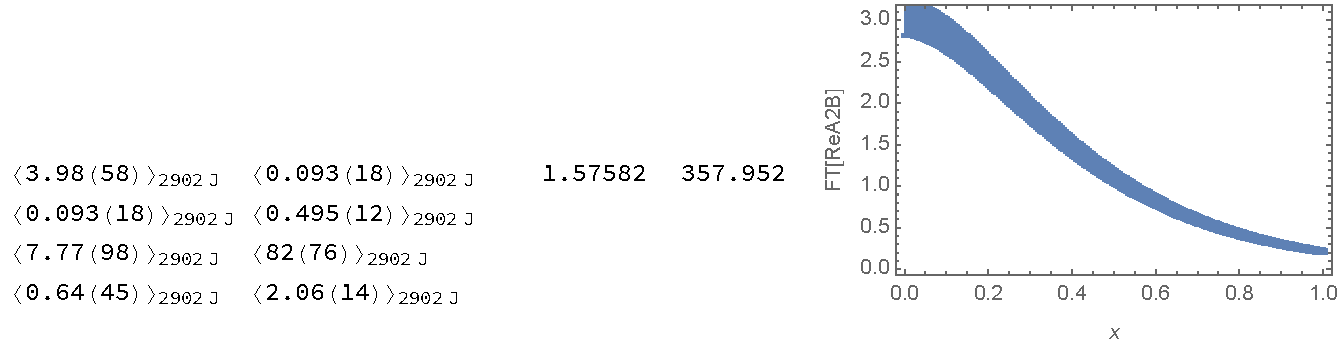
\includegraphics[width=\linewidth,height=.72\textheight,keepaspectratio]{fitting/A2BfitFT_eta_Asymptotic_P1__block6_part2.pdf}
\par\small $P_L=-1$, $|\vect b|\ge3a$, $6\le\eta\le10$. Original thesis table, enlarged without omitted rows.

\figsrc{Thesis: PowerLaw\_etaAsymptotic; A2BfitFT\_eta\_Asymptotic\_P1}
\end{frame}

\begin{frame}{Wider Fourier-profile candidate diagnostics --- block 1, models}
\centering
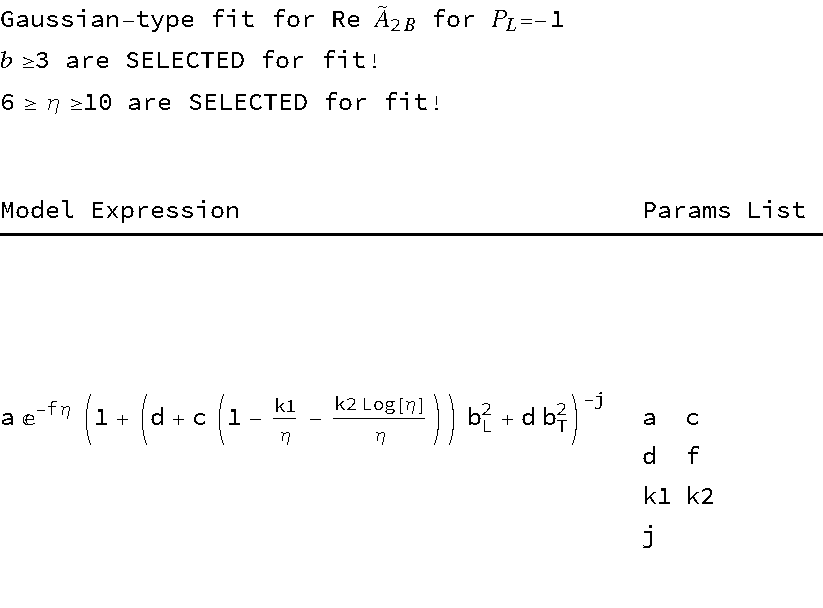
\includegraphics[width=\linewidth,height=.72\textheight,keepaspectratio]{fitting/A2Bfit_widerFT_eta_Asymptotic_P1__block1_part1.pdf}
\par\small $P_L=-1$, $|\vect b|\ge3a$, $6\le\eta\le10$. Original thesis table, enlarged without omitted rows.

\figsrc{Thesis: PowerLaw\_etaAsymptotic; A2Bfit\_widerFT\_eta\_Asymptotic\_P1}
\end{frame}

\begin{frame}{Wider Fourier-profile candidate diagnostics --- block 1, parameters and diagnostics}
\centering
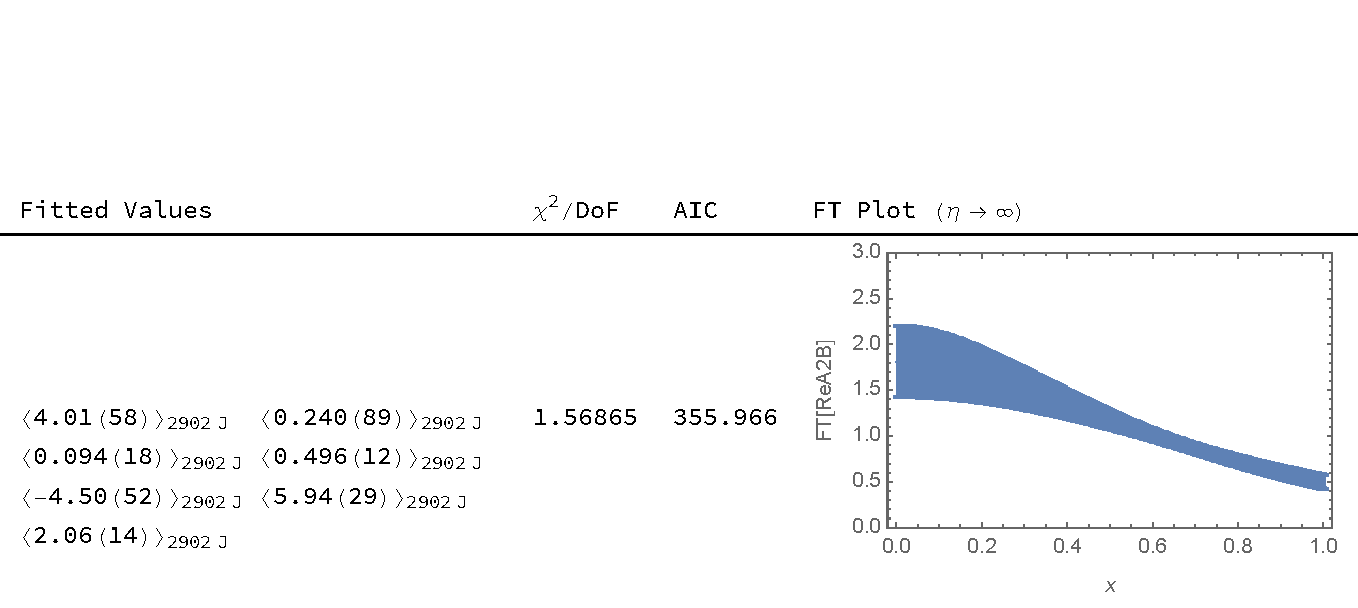
\includegraphics[width=\linewidth,height=.72\textheight,keepaspectratio]{fitting/A2Bfit_widerFT_eta_Asymptotic_P1__block1_part2.pdf}
\par\small $P_L=-1$, $|\vect b|\ge3a$, $6\le\eta\le10$. Original thesis table, enlarged without omitted rows.

\figsrc{Thesis: PowerLaw\_etaAsymptotic; A2Bfit\_widerFT\_eta\_Asymptotic\_P1}
\end{frame}

\begin{frame}{Wider Fourier-profile candidate diagnostics --- block 2, models}
\centering
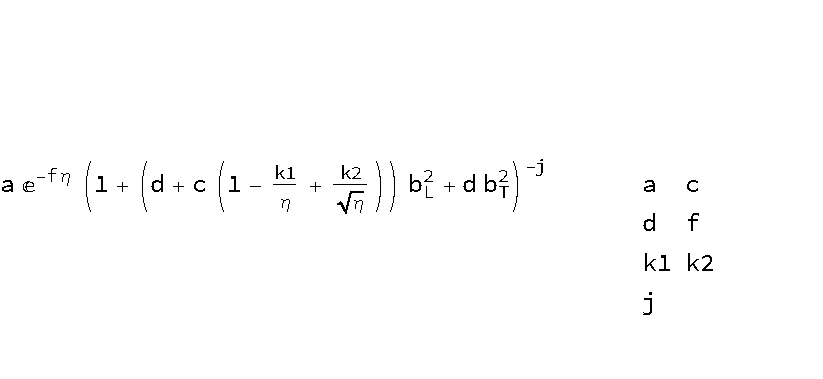
\includegraphics[width=\linewidth,height=.72\textheight,keepaspectratio]{fitting/A2Bfit_widerFT_eta_Asymptotic_P1__block2_part1.pdf}
\par\small $P_L=-1$, $|\vect b|\ge3a$, $6\le\eta\le10$. Original thesis table, enlarged without omitted rows.

\figsrc{Thesis: PowerLaw\_etaAsymptotic; A2Bfit\_widerFT\_eta\_Asymptotic\_P1}
\end{frame}

\begin{frame}{Wider Fourier-profile candidate diagnostics --- block 2, parameters and diagnostics}
\centering
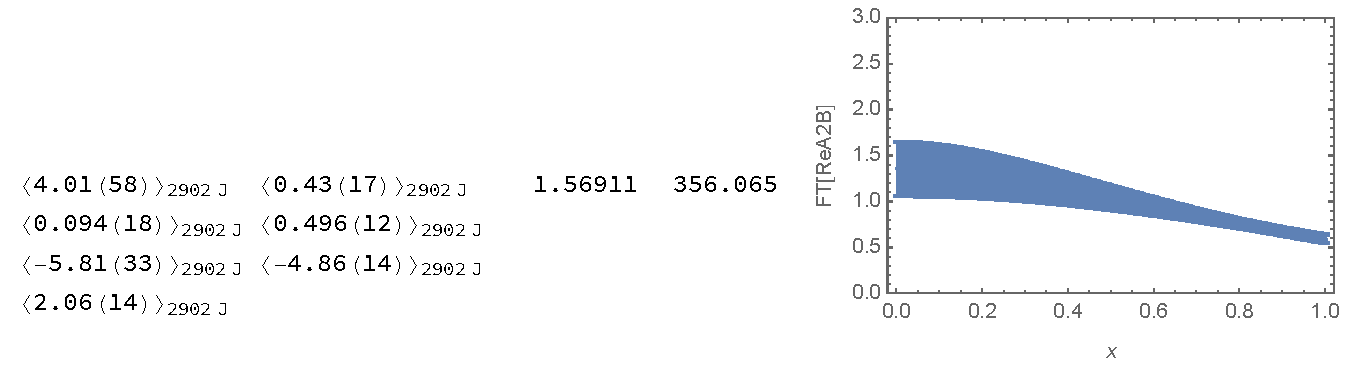
\includegraphics[width=\linewidth,height=.72\textheight,keepaspectratio]{fitting/A2Bfit_widerFT_eta_Asymptotic_P1__block2_part2.pdf}
\par\small $P_L=-1$, $|\vect b|\ge3a$, $6\le\eta\le10$. Original thesis table, enlarged without omitted rows.

\figsrc{Thesis: PowerLaw\_etaAsymptotic; A2Bfit\_widerFT\_eta\_Asymptotic\_P1}
\end{frame}

\begin{frame}{Wider Fourier-profile candidate diagnostics --- block 3, models}
\centering
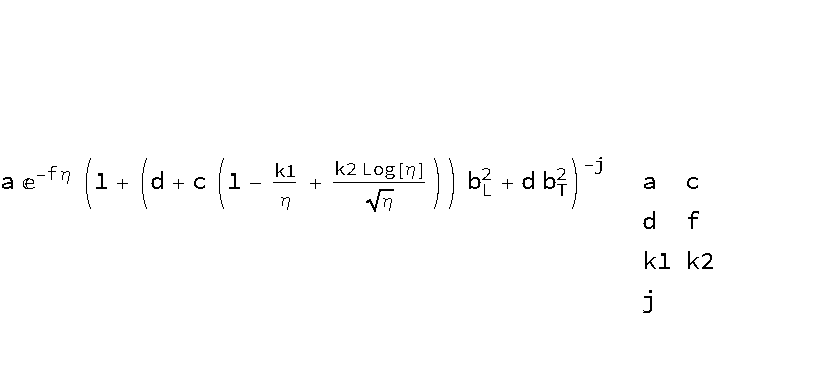
\includegraphics[width=\linewidth,height=.72\textheight,keepaspectratio]{fitting/A2Bfit_widerFT_eta_Asymptotic_P1__block3_part1.pdf}
\par\small $P_L=-1$, $|\vect b|\ge3a$, $6\le\eta\le10$. Original thesis table, enlarged without omitted rows.

\figsrc{Thesis: PowerLaw\_etaAsymptotic; A2Bfit\_widerFT\_eta\_Asymptotic\_P1}
\end{frame}

\begin{frame}{Wider Fourier-profile candidate diagnostics --- block 3, parameters and diagnostics}
\centering
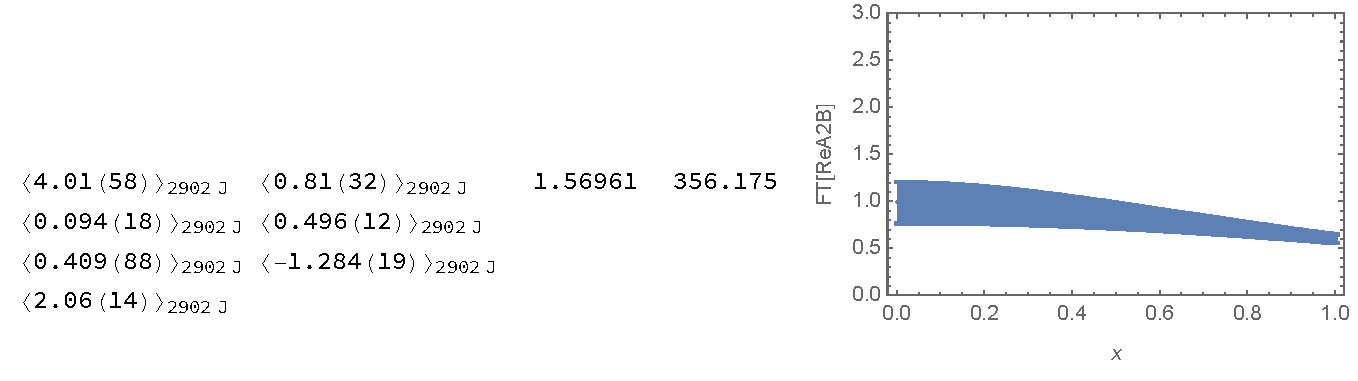
\includegraphics[width=\linewidth,height=.72\textheight,keepaspectratio]{fitting/A2Bfit_widerFT_eta_Asymptotic_P1__block3_part2.pdf}
\par\small $P_L=-1$, $|\vect b|\ge3a$, $6\le\eta\le10$. Original thesis table, enlarged without omitted rows.

\figsrc{Thesis: PowerLaw\_etaAsymptotic; A2Bfit\_widerFT\_eta\_Asymptotic\_P1}
\end{frame}

\begin{frame}{Wider Fourier-profile candidate diagnostics --- block 4, models}
\centering
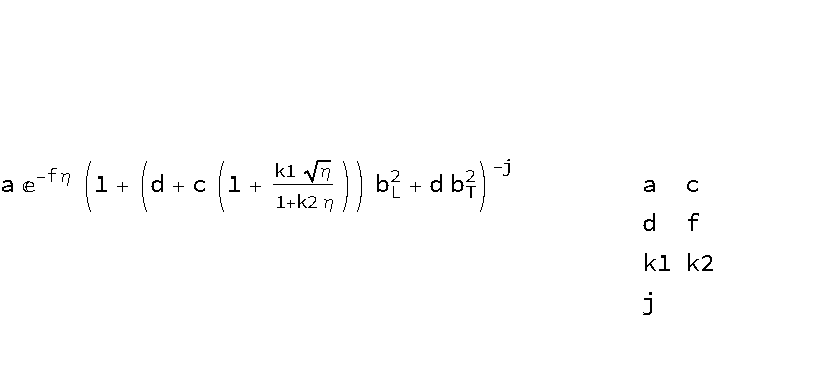
\includegraphics[width=\linewidth,height=.72\textheight,keepaspectratio]{fitting/A2Bfit_widerFT_eta_Asymptotic_P1__block4_part1.pdf}
\par\small $P_L=-1$, $|\vect b|\ge3a$, $6\le\eta\le10$. Original thesis table, enlarged without omitted rows.

\figsrc{Thesis: PowerLaw\_etaAsymptotic; A2Bfit\_widerFT\_eta\_Asymptotic\_P1}
\end{frame}

\begin{frame}{Wider Fourier-profile candidate diagnostics --- block 4, parameters and diagnostics}
\centering
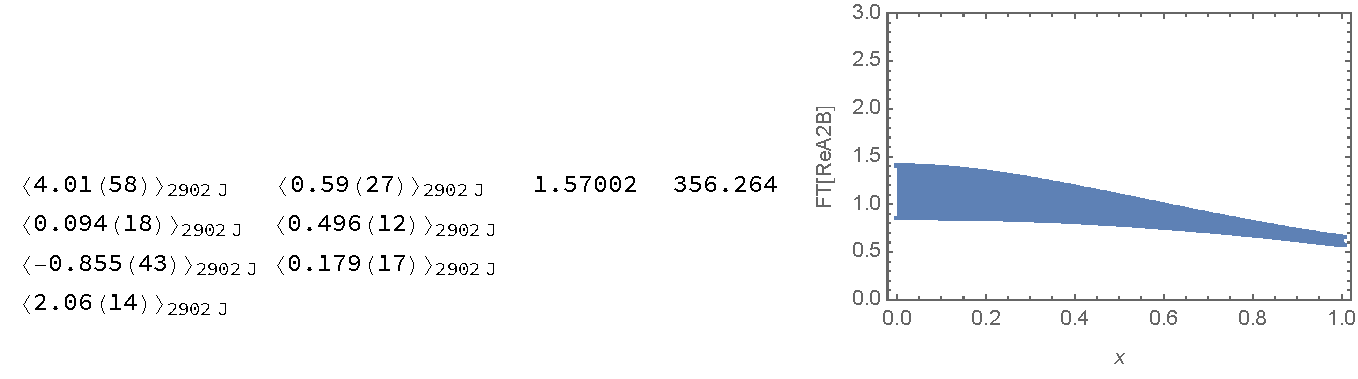
\includegraphics[width=\linewidth,height=.72\textheight,keepaspectratio]{fitting/A2Bfit_widerFT_eta_Asymptotic_P1__block4_part2.pdf}
\par\small $P_L=-1$, $|\vect b|\ge3a$, $6\le\eta\le10$. Original thesis table, enlarged without omitted rows.

\figsrc{Thesis: PowerLaw\_etaAsymptotic; A2Bfit\_widerFT\_eta\_Asymptotic\_P1}
\end{frame}

\begin{frame}{All ten asymptotic width candidates (1/2)}
\begin{align*}c_{1}(\eta)&=c(1-k_1/\eta)\\[2mm]
c_{2}(\eta)&=c(1-k_1/\eta-k_2/\eta^2)\\[2mm]
c_{3}(\eta)&=c(1-k_1/\eta-k_2/\eta^2-k_3/\eta^3)\\[2mm]
c_{4}(\eta)&=c(1-k_1\log\eta/\eta)\\[2mm]
c_{5}(\eta)&=c(1-k_1/\eta-k_2\log\eta/\eta)\\[2mm]\end{align*}
\figsrc{Thesis: Fitting Methodologies and Stability Analysis}
\end{frame}

\begin{frame}{All ten asymptotic width candidates (2/2)}
\begin{align*}c_{6}(\eta)&=c(1-k_1/\eta+k_2/\sqrt\eta)\\[2mm]
c_{7}(\eta)&=c(1-k_1/\eta+k_2\log\eta/\sqrt\eta)\\[2mm]
c_{8}(\eta)&=c(1+k_1\sqrt\eta/(1+k_2\eta))\\[2mm]
c_{9}(\eta)&=c(1-k_1/\eta^{0.2}+k_2/\eta^{0.8})\\[2mm]
c_{10}(\eta)&=c(1-k_1/\eta^{0.3}+k_2/\eta^{0.7})\\[2mm]\end{align*}
\figsrc{Thesis: Fitting Methodologies and Stability Analysis}
\end{frame}

\begin{frame}{Fixed-$\eta$ fits: $\tAmp_{2B}^{\mathrm{Re}}$}
\centering
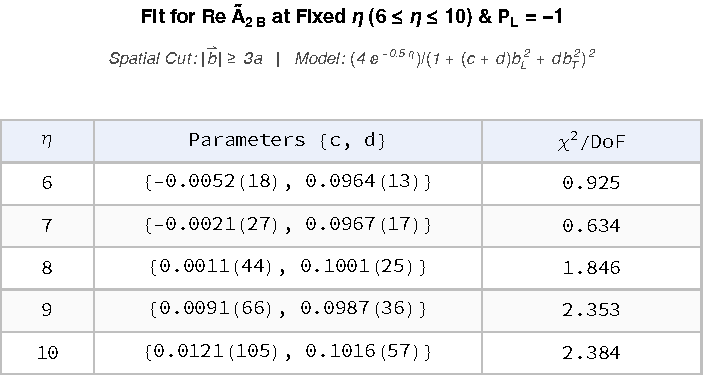
\includegraphics[width=\linewidth,height=.70\textheight,keepaspectratio]{fitting/LorentzianFixedA_P-1_b3.pdf}
\par\small Fix $a=4$, $j=2$, $f=0.5$ to isolate $c(\eta)$ and $d(\eta)$.

\figsrc{Thesis: Gaussian\_type\_fit\_Real\_A2B; LorentzianFixedA\_P-1\_b3}
\end{frame}

\begin{frame}{$c_1$ through $c_{10}$ against the extracted widths}
\centering
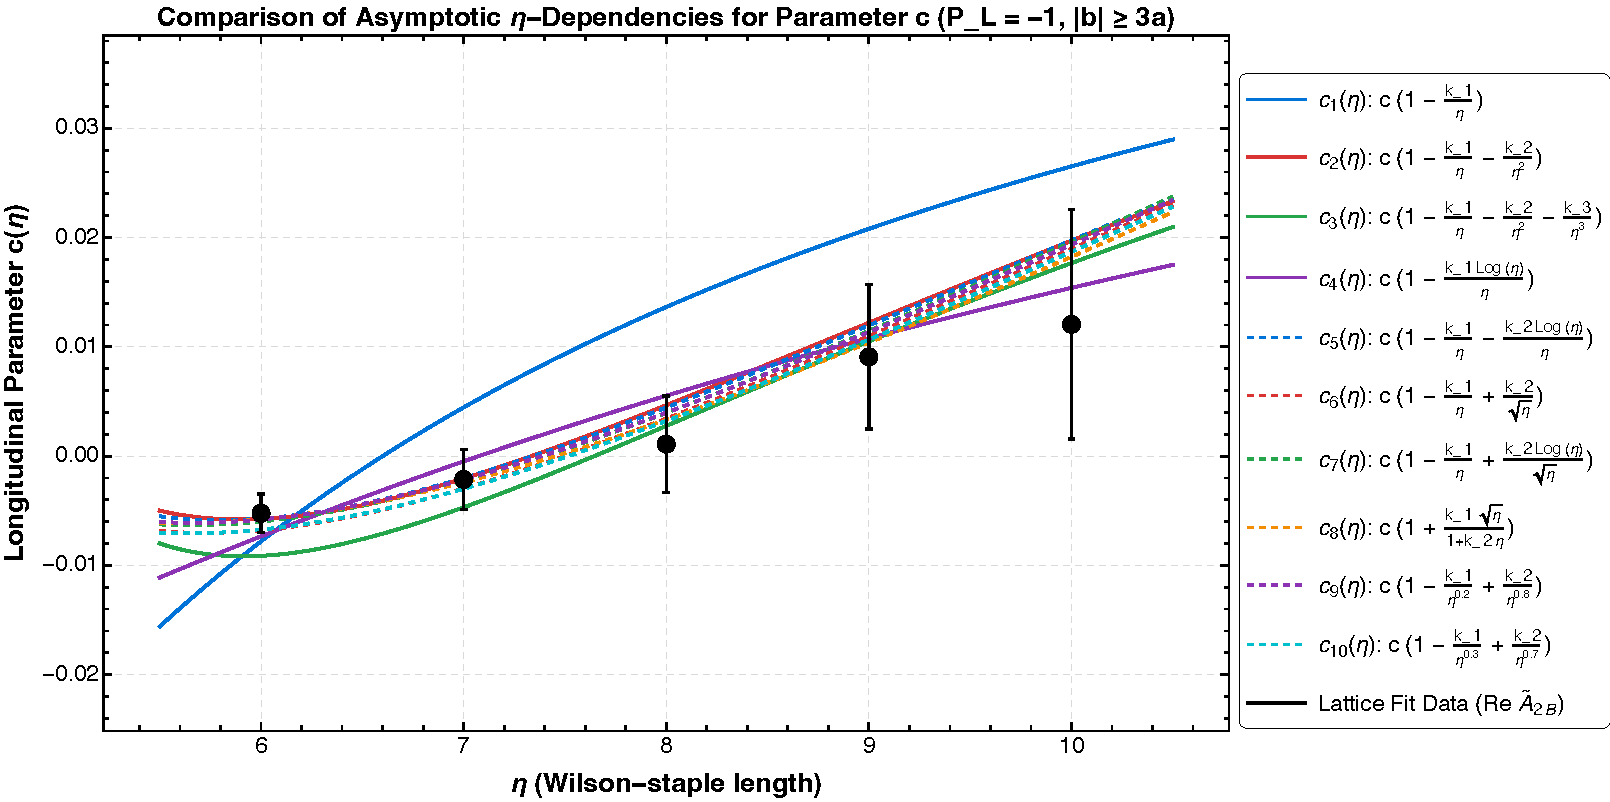
\includegraphics[width=\linewidth,height=.70\textheight,keepaspectratio]{fitting/A2B_c_eta_AllAsymptoticModels_P1.pdf}
\par\small Several forms describe the measured staple range similarly.

\figsrc{Thesis: PowerLaw\_etaAsymptotic; A2B\_c\_eta\_AllAsymptoticModels\_P1}
\end{frame}

\begin{frame}{Transverse width: $\tAmp_{2B}^{\mathrm{Re}}$}
\centering
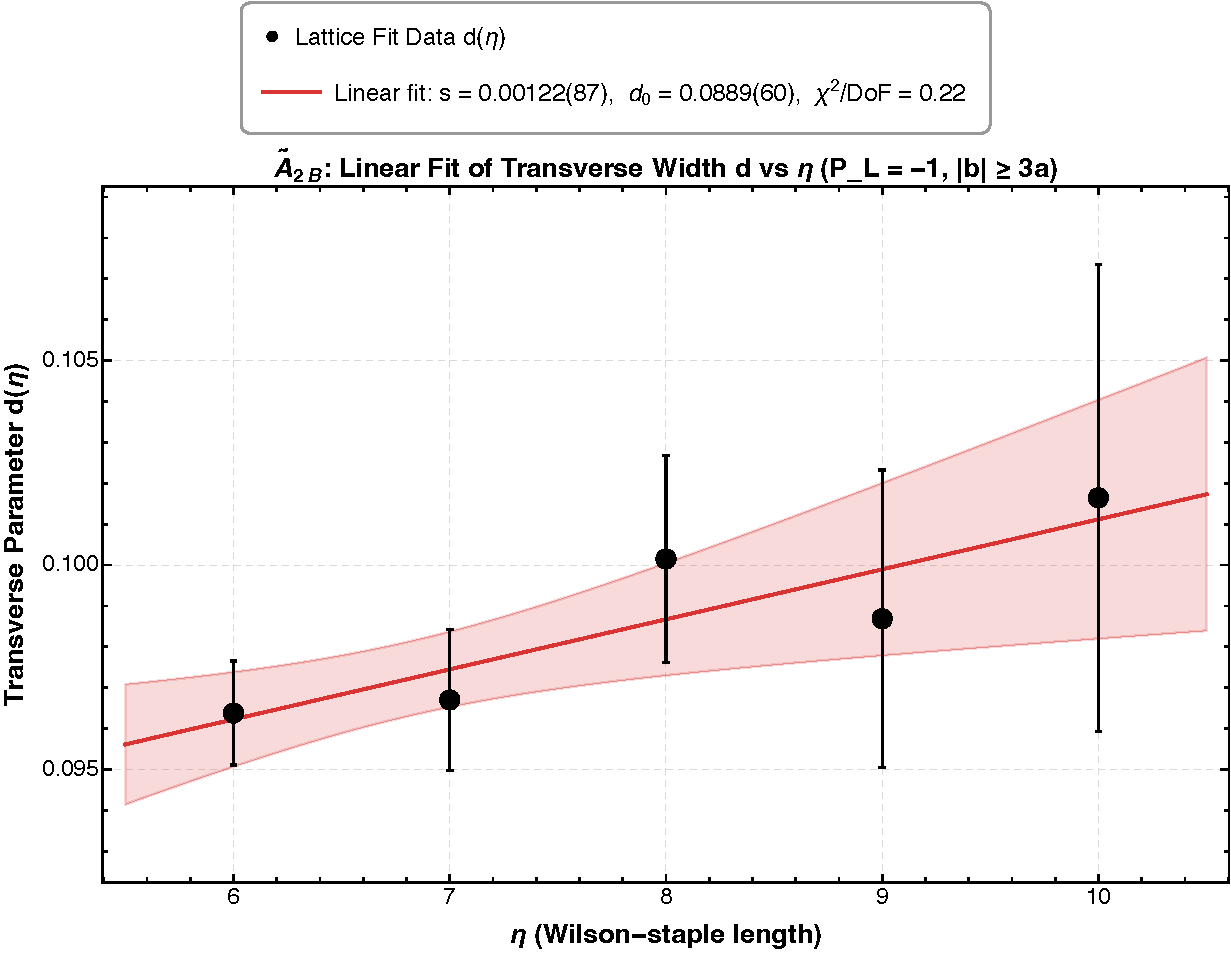
\includegraphics[width=\linewidth,height=.70\textheight,keepaspectratio]{fitting/A2B_d_eta_Independence_P1.pdf}
\par\small $s=0.00122(87)$, $d_0=0.0889(60)$, $\chi^2/\mathrm{dof}=0.22$: keep $d$ constant.

\figsrc{Thesis: PowerLaw\_etaAsymptotic; A2B\_d\_eta\_Independence\_P1}
\end{frame}

\begin{frame}{Fixed-$\eta$ fits: $\tAmp_{12B}^{\mathrm{Re}}$}
\centering
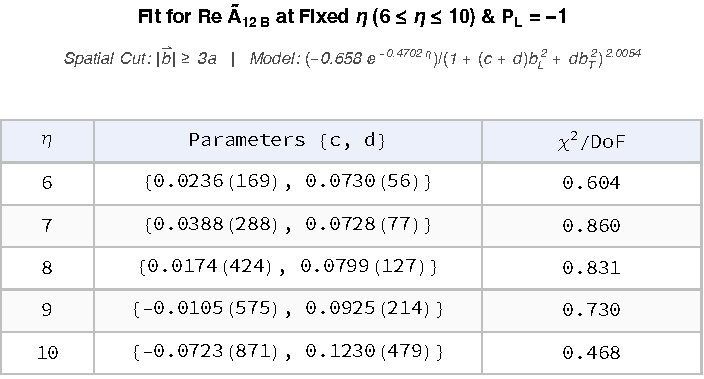
\includegraphics[width=\linewidth,height=.70\textheight,keepaspectratio]{fitting/LorentzianFixed_ReA12B_P-1_b3.pdf}
\par\small All five staple slices and their fit statistics.

\figsrc{Thesis: Gaussian\_type\_fit\_Real\_A2B; LorentzianFixed\_ReA12B\_P-1\_b3}
\end{frame}

\begin{frame}{Fixed-$\eta$ fits: $\tAmp_{2B}^{\mathrm{Im}}$}
\centering
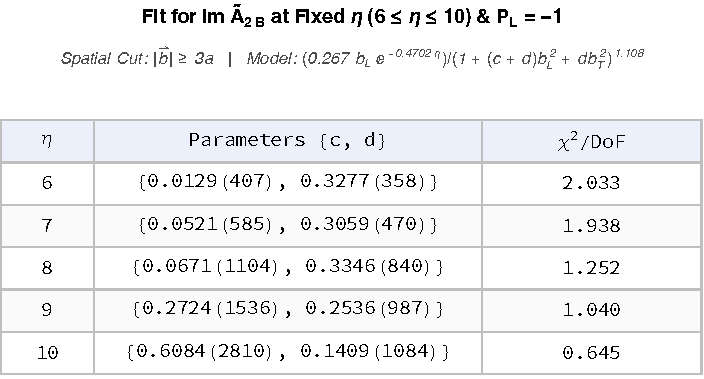
\includegraphics[width=\linewidth,height=.70\textheight,keepaspectratio]{fitting/LorentzianFixed_ImA2B_P-1_b3.pdf}
\par\small All five staple slices and their fit statistics.

\figsrc{Thesis: Gaussian\_type\_fit\_Real\_A2B; LorentzianFixed\_ImA2B\_P-1\_b3}
\end{frame}

\begin{frame}{Staple dependence of $c$: $\tAmp_{12B}^{\mathrm{Re}}$}
\centering
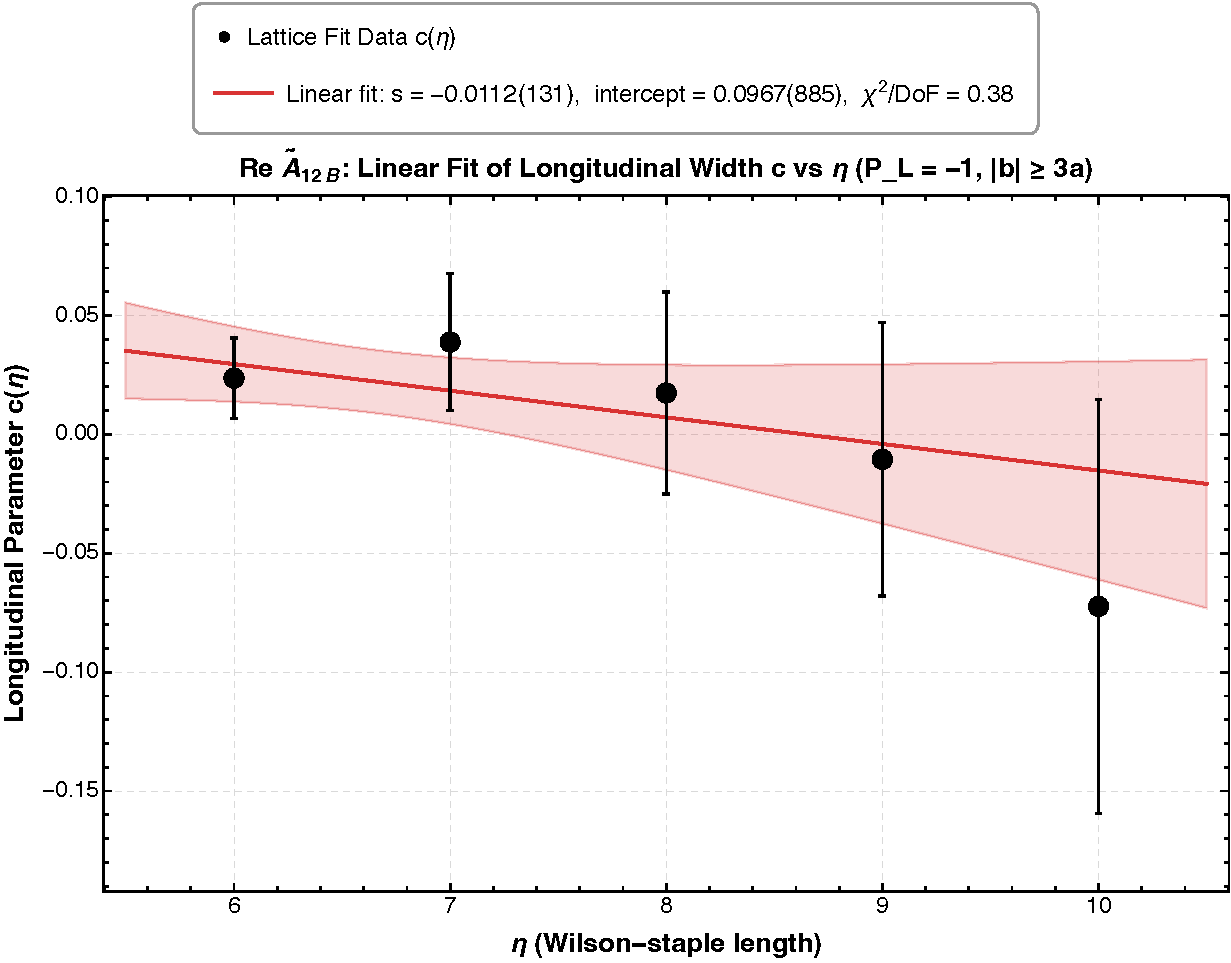
\includegraphics[width=\linewidth,height=.70\textheight,keepaspectratio]{fitting/ReA12B_c_eta_Independence_P1.pdf}
\par\small Slopes: $s_c=-0.0112(131)$, $s_d=0.0052(48)$; both compatible with zero.

\figsrc{Thesis: PowerLaw\_etaAsymptotic; ReA12B\_c\_eta\_Independence\_P1}
\end{frame}

\begin{frame}{Staple dependence of $d$: $\tAmp_{12B}^{\mathrm{Re}}$}
\centering
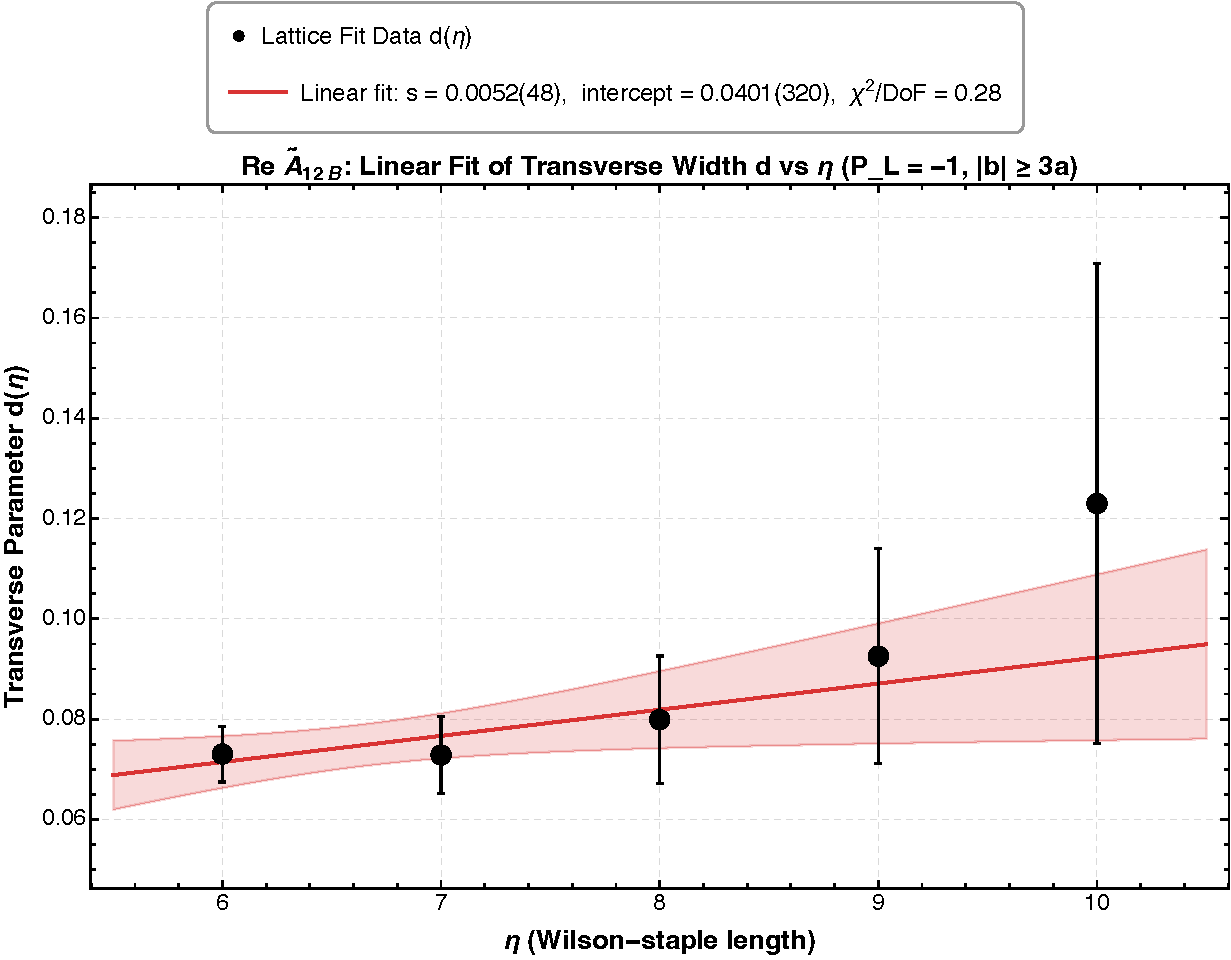
\includegraphics[width=\linewidth,height=.70\textheight,keepaspectratio]{fitting/ReA12B_d_eta_Independence_P1.pdf}
\par\small Slopes: $s_c=-0.0112(131)$, $s_d=0.0052(48)$; both compatible with zero.

\figsrc{Thesis: PowerLaw\_etaAsymptotic; ReA12B\_d\_eta\_Independence\_P1}
\end{frame}

\begin{frame}{Staple dependence of $c$: $\tAmp_{2B}^{\mathrm{Im}}$}
\centering
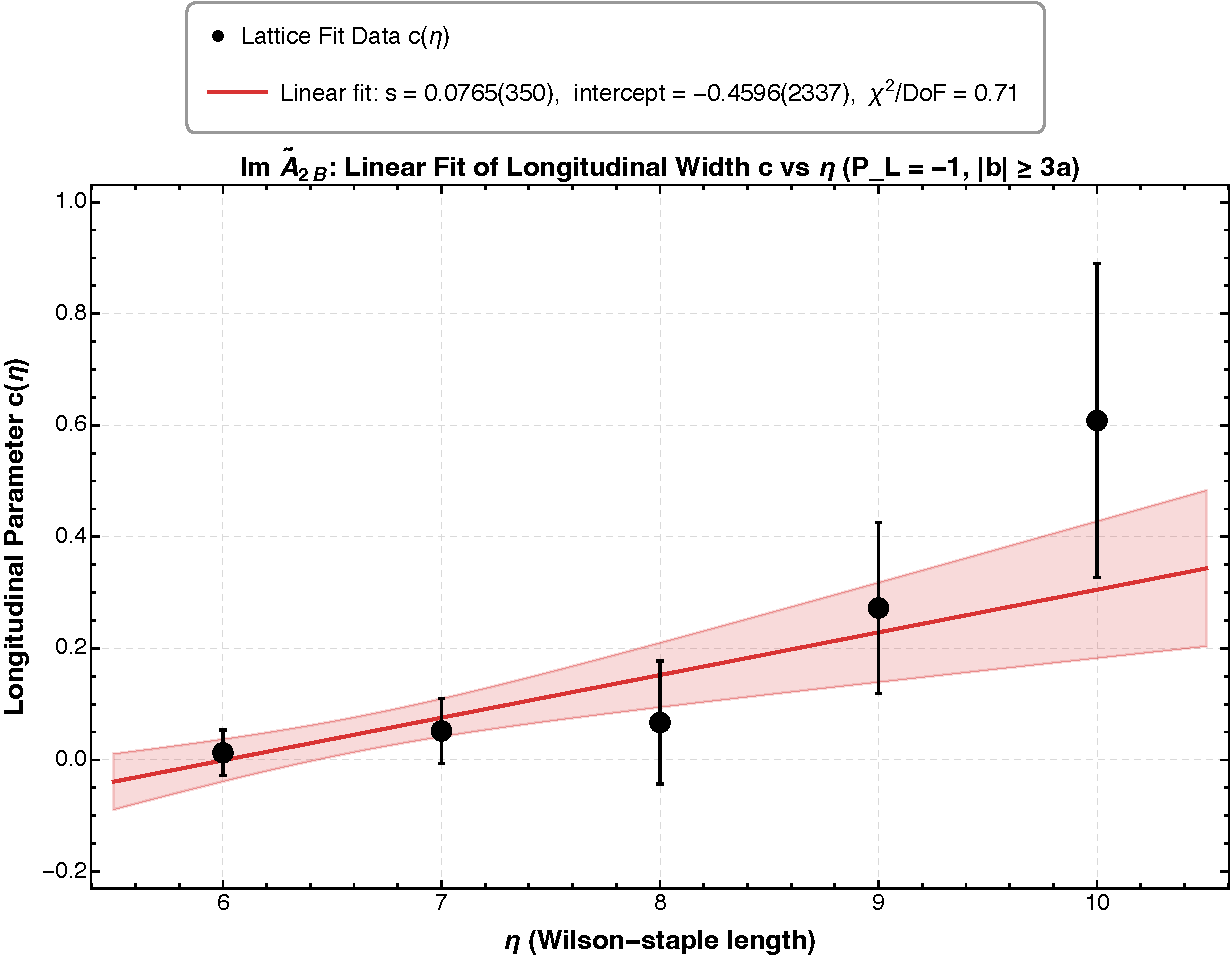
\includegraphics[width=\linewidth,height=.70\textheight,keepaspectratio]{fitting/ImA2B_c_eta_Independence_P1.pdf}
\par\small Slopes: $s_c=0.0765(350)$, $s_d=-0.0316(219)$; $c$ is about $2.2\sigma$ from zero. Constant widths are a modeling choice under these uncertainties.

\figsrc{Thesis: PowerLaw\_etaAsymptotic; ImA2B\_c\_eta\_Independence\_P1}
\end{frame}

\begin{frame}{Staple dependence of $d$: $\tAmp_{2B}^{\mathrm{Im}}$}
\centering
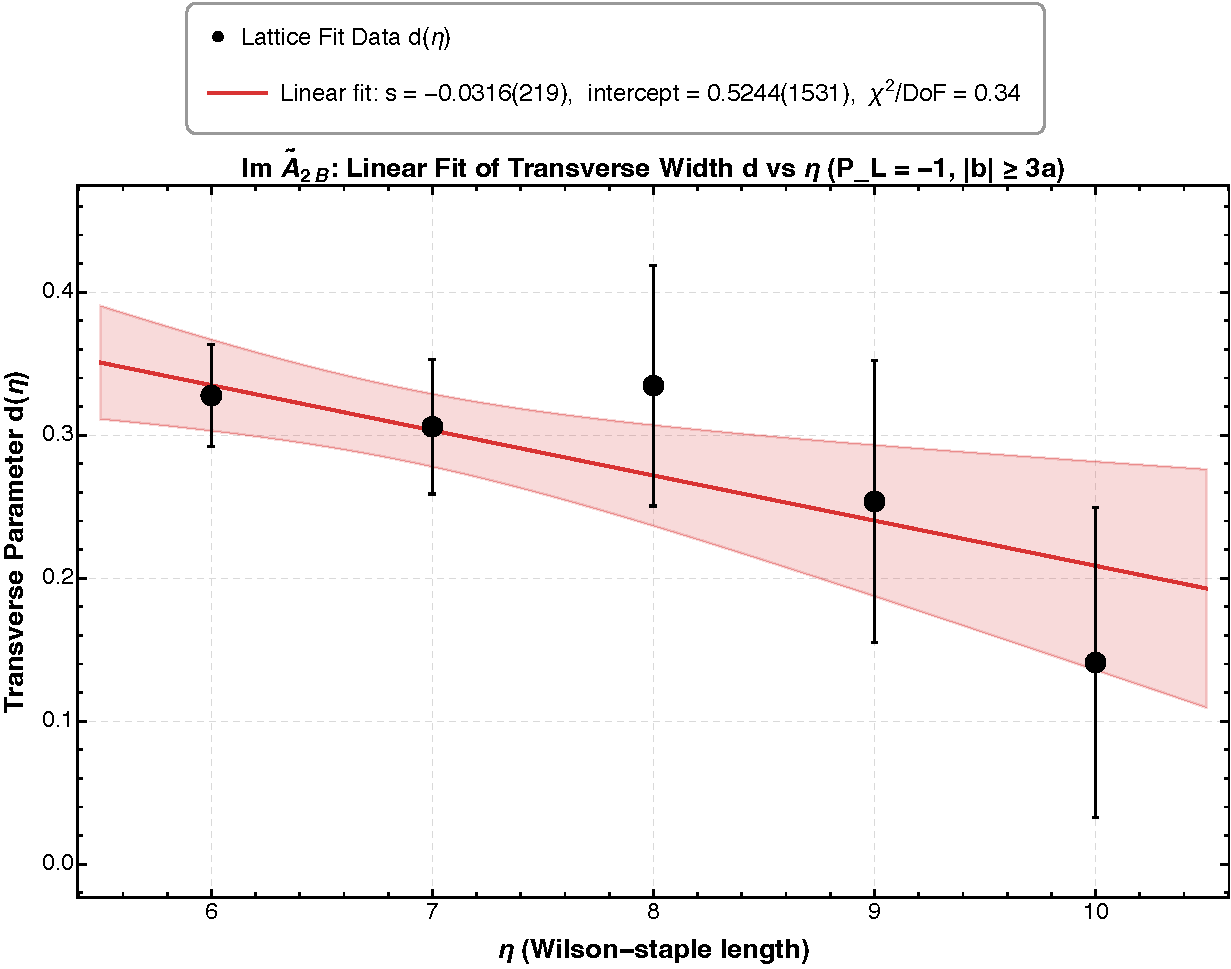
\includegraphics[width=\linewidth,height=.70\textheight,keepaspectratio]{fitting/ImA2B_d_eta_Independence_P1.pdf}
\par\small Slopes: $s_c=0.0765(350)$, $s_d=-0.0316(219)$; $c$ is about $2.2\sigma$ from zero. Constant widths are a modeling choice under these uncertainties.

\figsrc{Thesis: PowerLaw\_etaAsymptotic; ImA2B\_d\_eta\_Independence\_P1}
\end{frame}

\begin{frame}{Candidate selection combines several diagnostics}

\begin{itemize}
\item Fit quality, parameter stability, and AIC distinguish candidates with similar fixed-$\eta$ curves.
\item The thesis favors $c_2(\eta)=c(1-k_1/\eta-k_2/\eta^2)$ after examining the Fourier profile jointly with the imaginary amplitude.
\item For positive $x$, $\bar q(x)=-f_1(-x)$. The thesis uses suppression at $x\lesssim-0.2$ as a model-selection criterion for the negative-$x$ contribution.
\item Compare the integrated shift with previous $\nu=0$ lattice calculations; both real amplitudes and the imaginary unpolarized contribution enter the finite-$x$ integrals.
\end{itemize}
\[\langle k_y\rangle_{TU}^{[1]}=m_N\frac{\int dx\,\tilde f_{1T}^{\perp(1)}}{\int dx\,\tilde f_1^{(0)}}.\]
\figsrc{Thesis: Fitting Methodologies and Stability Analysis}
\end{frame}

\begin{frame}{The selected three-amplitude model}

\begin{align*}
\tAmp_{2B}^{\mathrm{Re}}&=\frac{a e^{-f\eta}}{[1+(d+c(1-k_1/\eta-k_2/\eta^2))b_L^2+db_T^2]^j},\\[3mm]
\tAmp_{12B}^{\mathrm{Re}}&=\frac{-a'e^{-f\eta}}{[1+(c'+d')b_L^2+d'b_T^2]^{j'}},\\[3mm]
\tAmp_{2B}^{\mathrm{Im}}&=\frac{a''b_L e^{-f\eta}}{[1+(c''+d'')b_L^2+d''b_T^2]^{j''}}.
\end{align*}
Shared $f$; independent spatial shape parameters for each amplitude.\par
$\tAmp_{12B}^{\mathrm{Im}}$ is omitted because the measured signal is consistent with zero.
\figsrc{Thesis: Fitting Methodologies and Stability Analysis}
\end{frame}

\begin{frame}{Full covariance in the simultaneous fit}

\[\bar y_i=\frac1{N_J}\sum_{k=1}^{N_J}y_i^{(k)},\qquad
C_{ij}=\frac{N_J-1}{N_J}\sum_{k=1}^{N_J}(y_i^{(k)}-\bar y_i)(y_j^{(k)}-\bar y_j).\]
\[\chi^2_{\rm data}(\mathbf p)=\sum_{i,j}[\bar y_i-F_i(\mathbf p)]C^{-1}_{ij}[\bar y_j-F_j(\mathbf p)].\]
\begin{itemize}
\item The combined data vector includes all retained coordinates and all three amplitudes at one momentum.
\item Cross-correlations matter because amplitudes use the same gauge configurations. Ignoring them changes the weighting and can misestimate uncertainties.
\item The implementation uses Gaussian priors and minimizes $\chi^2_{\rm aug}$, not just $\chi^2_{\rm data}$. Jackknife refits propagate the resulting parameter fluctuations.
\end{itemize}
\figsrc{Thesis: Fitting Methodologies and Stability Analysis}
\end{frame}

\begin{frame}{Actual simultaneous-fit objective and priors}
\[\chi^2_{\rm aug}=\chi^2_{\rm data}+\sum_{r=1}^{15}\left(\frac{p_r-\mu_r}{\sigma_r}\right)^2,
\qquad\sigma_r=0.05\quad\text{for all 15 parameters}.\]
\small\renewcommand{\arraystretch}{1.4}
\begin{tabular}{ll|ll|ll}\toprule
Real unpolarized & $\mu$ & Imaginary unpolarized & $\mu$ & Real Sivers / shared & $\mu$\\\midrule
$a$ & $4.01$ & $a''$ & $0.26$ & $a'$ & $0.6$\\
$c$ & $0.146$ & $c''$ & $0.3$ & $c'$ & $0.02$\\
$d$ & $0.094$ & $d''$ & $0.2$ & $d'$ & $0.02$\\
$k_1$ & $12.27$ & $j''$ & $1$ & $j'$ & $2$\\
$k_2$ & $-36.2$ & & & $f$ & $0.5$\\
$j$ & $2.06$ & & & & \\\bottomrule
\end{tabular}
\par\medskip All parameters are prior-constrained. The reported \texttt{lsqfit} statistic is $\chi^2_{\rm aug}/N_{\rm data}$; its degrees of freedom count includes the prior observations. It is not directly the same statistic as the earlier unregularized candidate fits.
\figsrc{Source: save\_h5\_A12B\_A2B/SimultaniousFit/SimultaneousFit\_A12bA2B.py, lines 197--247}
\end{frame}
\begin{frame}{Fourier continuation and integrability conditions}

\[D_R=[1+c(1-k_1/\eta-k_2/\eta^2)\nu^2/P_L^2+db^2]^j,\]
\[D_S=[1+c'\nu^2/P_L^2+d'b^2]^{j'},\qquad
D_I=[1+c''\nu^2/P_L^2+d''b^2]^{j''}.\]
\begin{itemize}
\item Cancel the common $e^{-f\eta}$ in the ratio; then take $\eta\to\infty$, so $c(\eta)\to c$.
\item For $A+B\nu^2$ with $A>0$, $B>0$, the even profile is absolutely integrable for $j>1/2$.
\item The odd profile $\nu(A+B\nu^2)^{-j''}$ needs $j''>1$ for absolute integrability. The highest-momentum fit lies close to this boundary.
\item Positivity must be checked in the continuation used for the transform; a positive spatial-grid denominator alone is insufficient.
\end{itemize}
\figsrc{Thesis: Fitting Methodologies and Stability Analysis}
\end{frame}

\begin{frame}{Real cosine and sine transforms: signs made explicit}

\begin{align*}
E(x,b^2)&=\int_{-\infty}^{\infty}\frac{d\nu}{2\pi}\cos(x\nu)R(\nu,b^2),\\
O(x,b^2)&=\int_{-\infty}^{\infty}\frac{d\nu}{2\pi}\sin(x\nu)I(\nu,b^2),\\
S(x,b^2)&=\int_{-\infty}^{\infty}\frac{d\nu}{2\pi}\cos(x\nu)S_0(\nu,b^2).
\end{align*}
$R,I,S_0$ denote the three selected amplitudes after removal of their common factor and the $\eta\to\infty$ limit.\par
\[\tilde f_1^{(0)}=2(E-O),\quad\tilde f_{1T}^{\perp(1)}=-2S,\quad
\langle k_y\rangle_{TU}=-m_N\frac{S}{E-O}.\]
The sine contribution $O$ is real; $i\int e^{ix\nu}I\,d\nu/(2\pi)=-O$.
\figsrc{Thesis: Fitting Methodologies and Stability Analysis}
\end{frame}

\begin{frame}{Integrated cross-checks and normalization}

\[\int_{-\infty}^{\infty}dx\,E(x,b^2)=R(0,b^2),\qquad
\int_{-\infty}^{\infty}dx\,O(x,b^2)=0,\]
\[m_N\frac{\int_{-\infty}^{\infty}dx\,\tilde f_{1T}^{\perp(1)}}
{\int_{-\infty}^{\infty}dx\,\tilde f_1^{(0)}}=-m_N\frac{S_0(0,b^2)}{R(0,b^2)}.\]
\begin{itemize}
\item The $1/(2\pi)$ Fourier normalization gives these identities.
\item The thesis tables compare $(-\infty,\infty)$, $[-1,1]$, $[-1,0]$, and $[0,1]$ at $b^2=9a^2$.
\item The ratio of integrals is distinct from the integral of the $x$-dependent ratio.
\item A common soft factor cancels in the shift; plotted individual transforms follow the thesis normalization convention.
\end{itemize}
\figsrc{Thesis: Fitting Methodologies and Stability Analysis}
\end{frame}

\begin{frame}{Simultaneous fit parameters: $P_L=-1$}
\small $|\vect b|\ge3a$, $6\le\eta\le10$; reported $\chi^2_{\rm aug}/N_{\rm data}=1.85(10)$.\par\medskip
\begin{columns}[t]\begin{column}{.32\textwidth}\centering $\tAmp_{2B}^{\mathrm{Re}}$\par\medskip\renewcommand{\arraystretch}{1.3}\begin{tabular}{cc}\toprule Parameter & Value\\\midrule
$a$ & $3.863(11)$ \\
$c$ & $0.336(40)$ \\
$d$ & $0.1630(74)$ \\
$k_1$ & $12.288(23)$ \\
$k_2$ & $-36.1965(45)$ \\
$j$ & $1.627(25)$ \\
$f$ & $0.4702(46)$ \\\bottomrule\end{tabular}\end{column}\begin{column}{.32\textwidth}\centering $\tAmp_{2B}^{\mathrm{Im}}$\par\medskip\renewcommand{\arraystretch}{1.3}\begin{tabular}{cc}\toprule Parameter & Value\\\midrule
$a''$ & $0.267(13)$ \\
$c''$ & $0.2253(69)$ \\
$d''$ & $0.2205(66)$ \\
$j''$ & $1.108(21)$ \\
$f$ & $0.4702(46)$ \\\bottomrule\end{tabular}\end{column}\begin{column}{.32\textwidth}\centering $\tAmp_{12B}^{\mathrm{Re}}$\par\medskip\renewcommand{\arraystretch}{1.3}\begin{tabular}{cc}\toprule Parameter & Value\\\midrule
$a'$ & $0.658(22)$ \\
$c'$ & $0.0773(46)$ \\
$d'$ & $0.0747(43)$ \\
$j'$ & $2.0054(90)$ \\
$f$ & $0.4702(46)$ \\\bottomrule\end{tabular}\end{column}\end{columns}
\figsrc{Thesis: SimultaneousFitsCov/Fit\_Table\_PL-1\_bmin3.tex}
\end{frame}

\begin{frame}{Global fit: $\tAmp_{2B}^{\mathrm{Re}}$, $P_L=-1$}
\centering
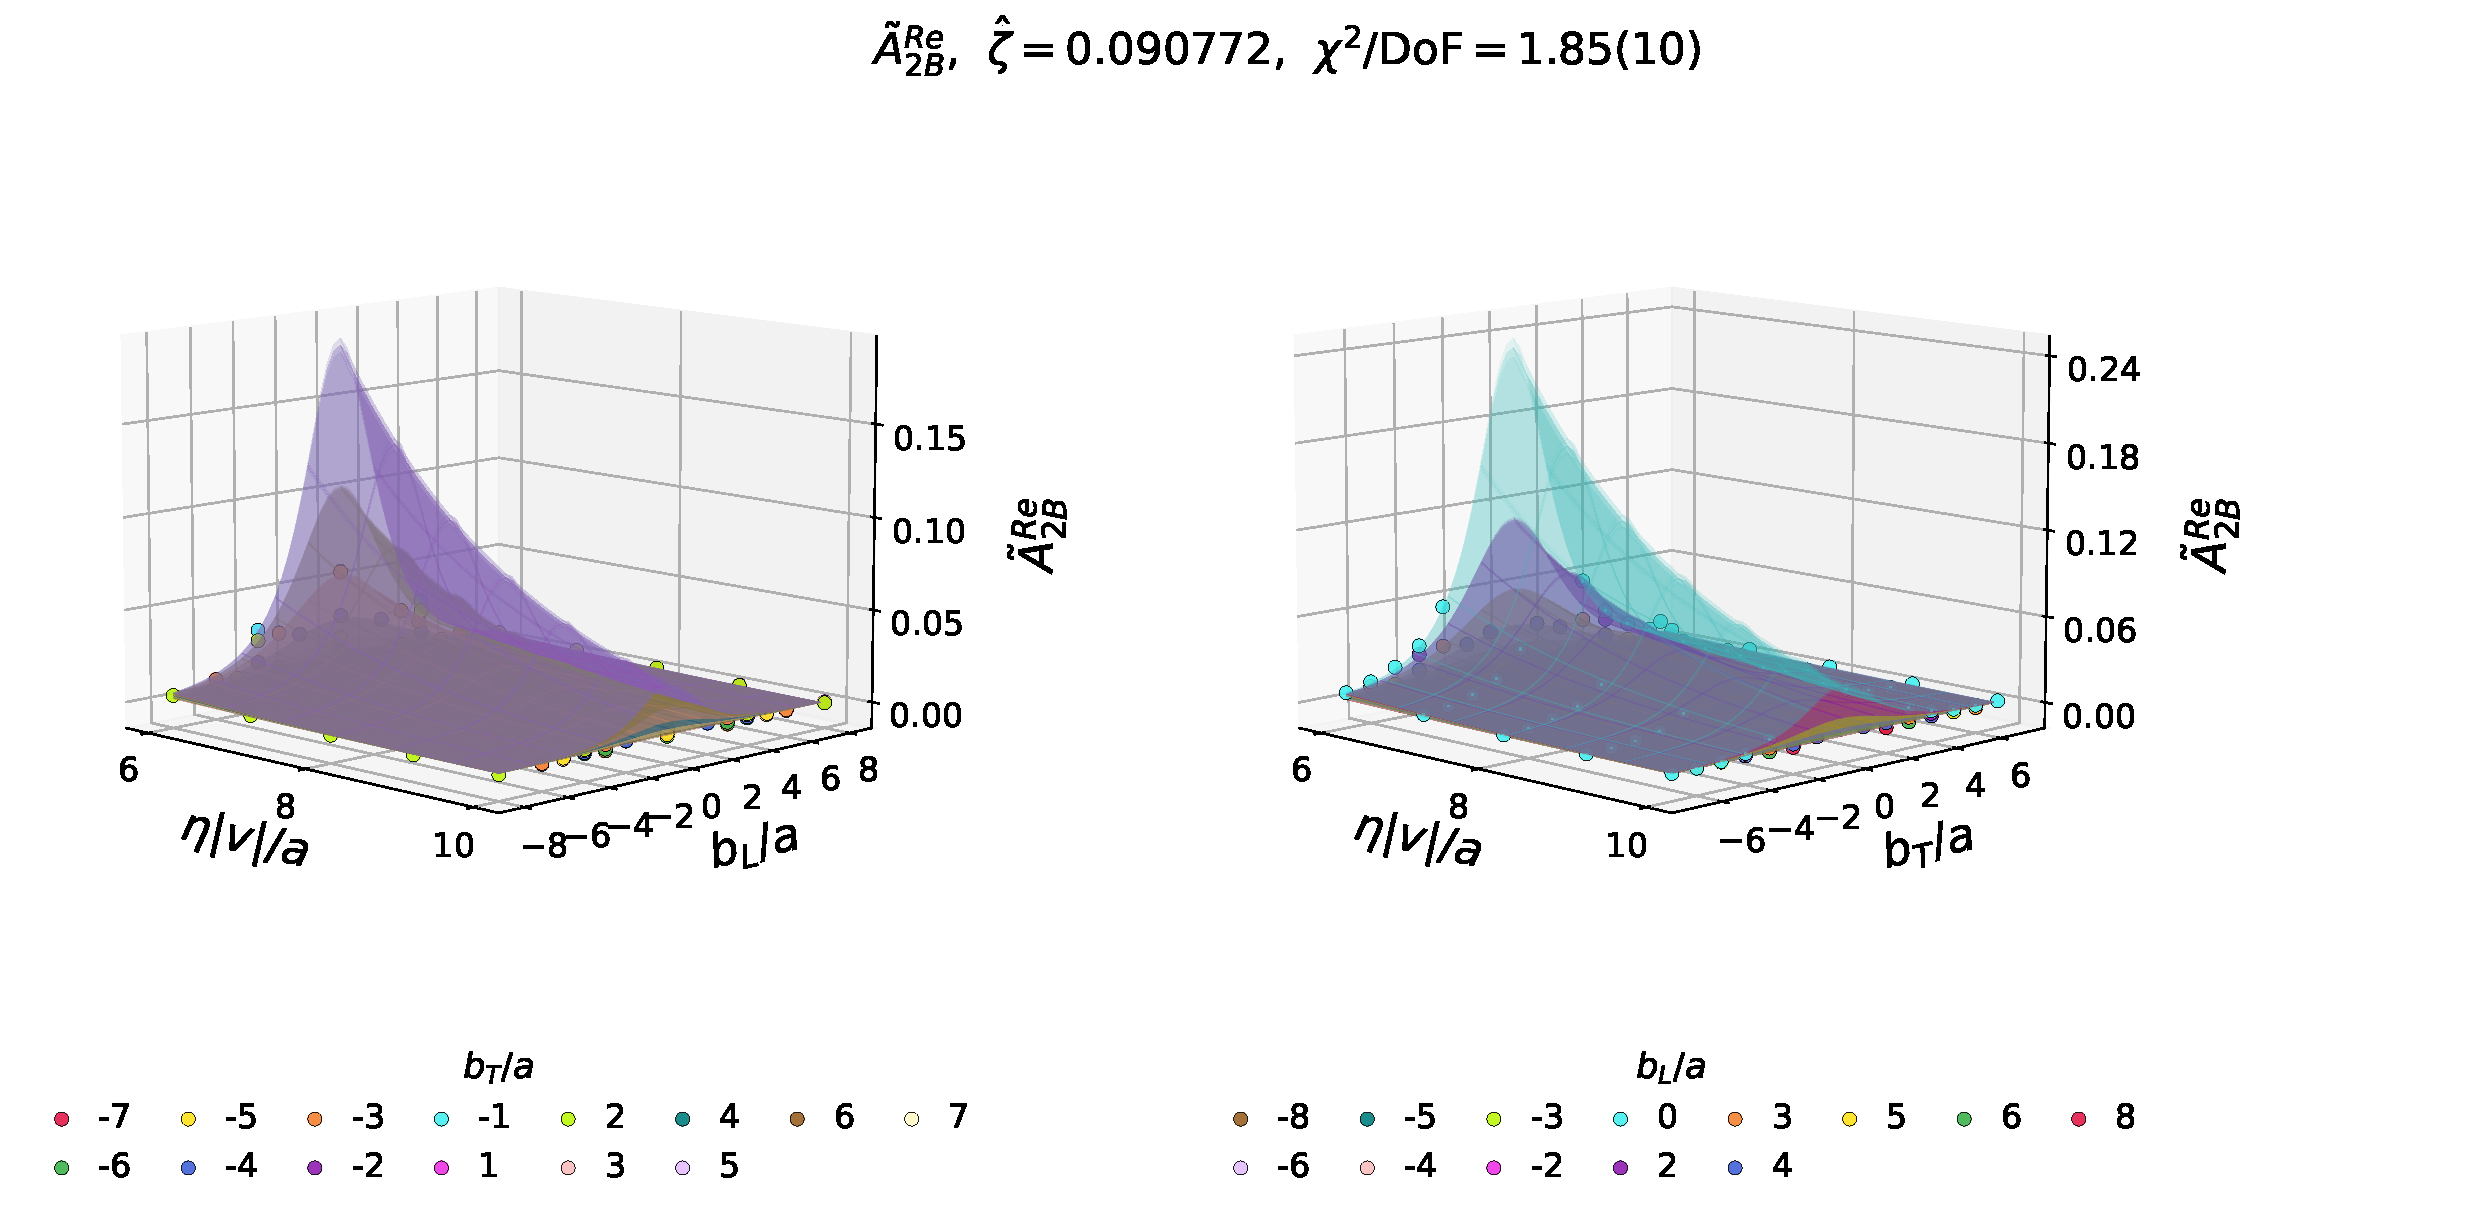
\includegraphics[width=\linewidth,height=.70\textheight,keepaspectratio]{fitting/ReA2B_PL-1_WithFit_3D.pdf}
\par\small Spatial coordinates: $(b_L,b_T,\eta)$. All panels and data overlays retained.

\figsrc{Thesis: plots; ReA2B\_PL-1\_WithFit\_3D}
\end{frame}

\begin{frame}{Global fit: $\tAmp_{2B}^{\mathrm{Re}}$, $P_L=-1$}
\centering
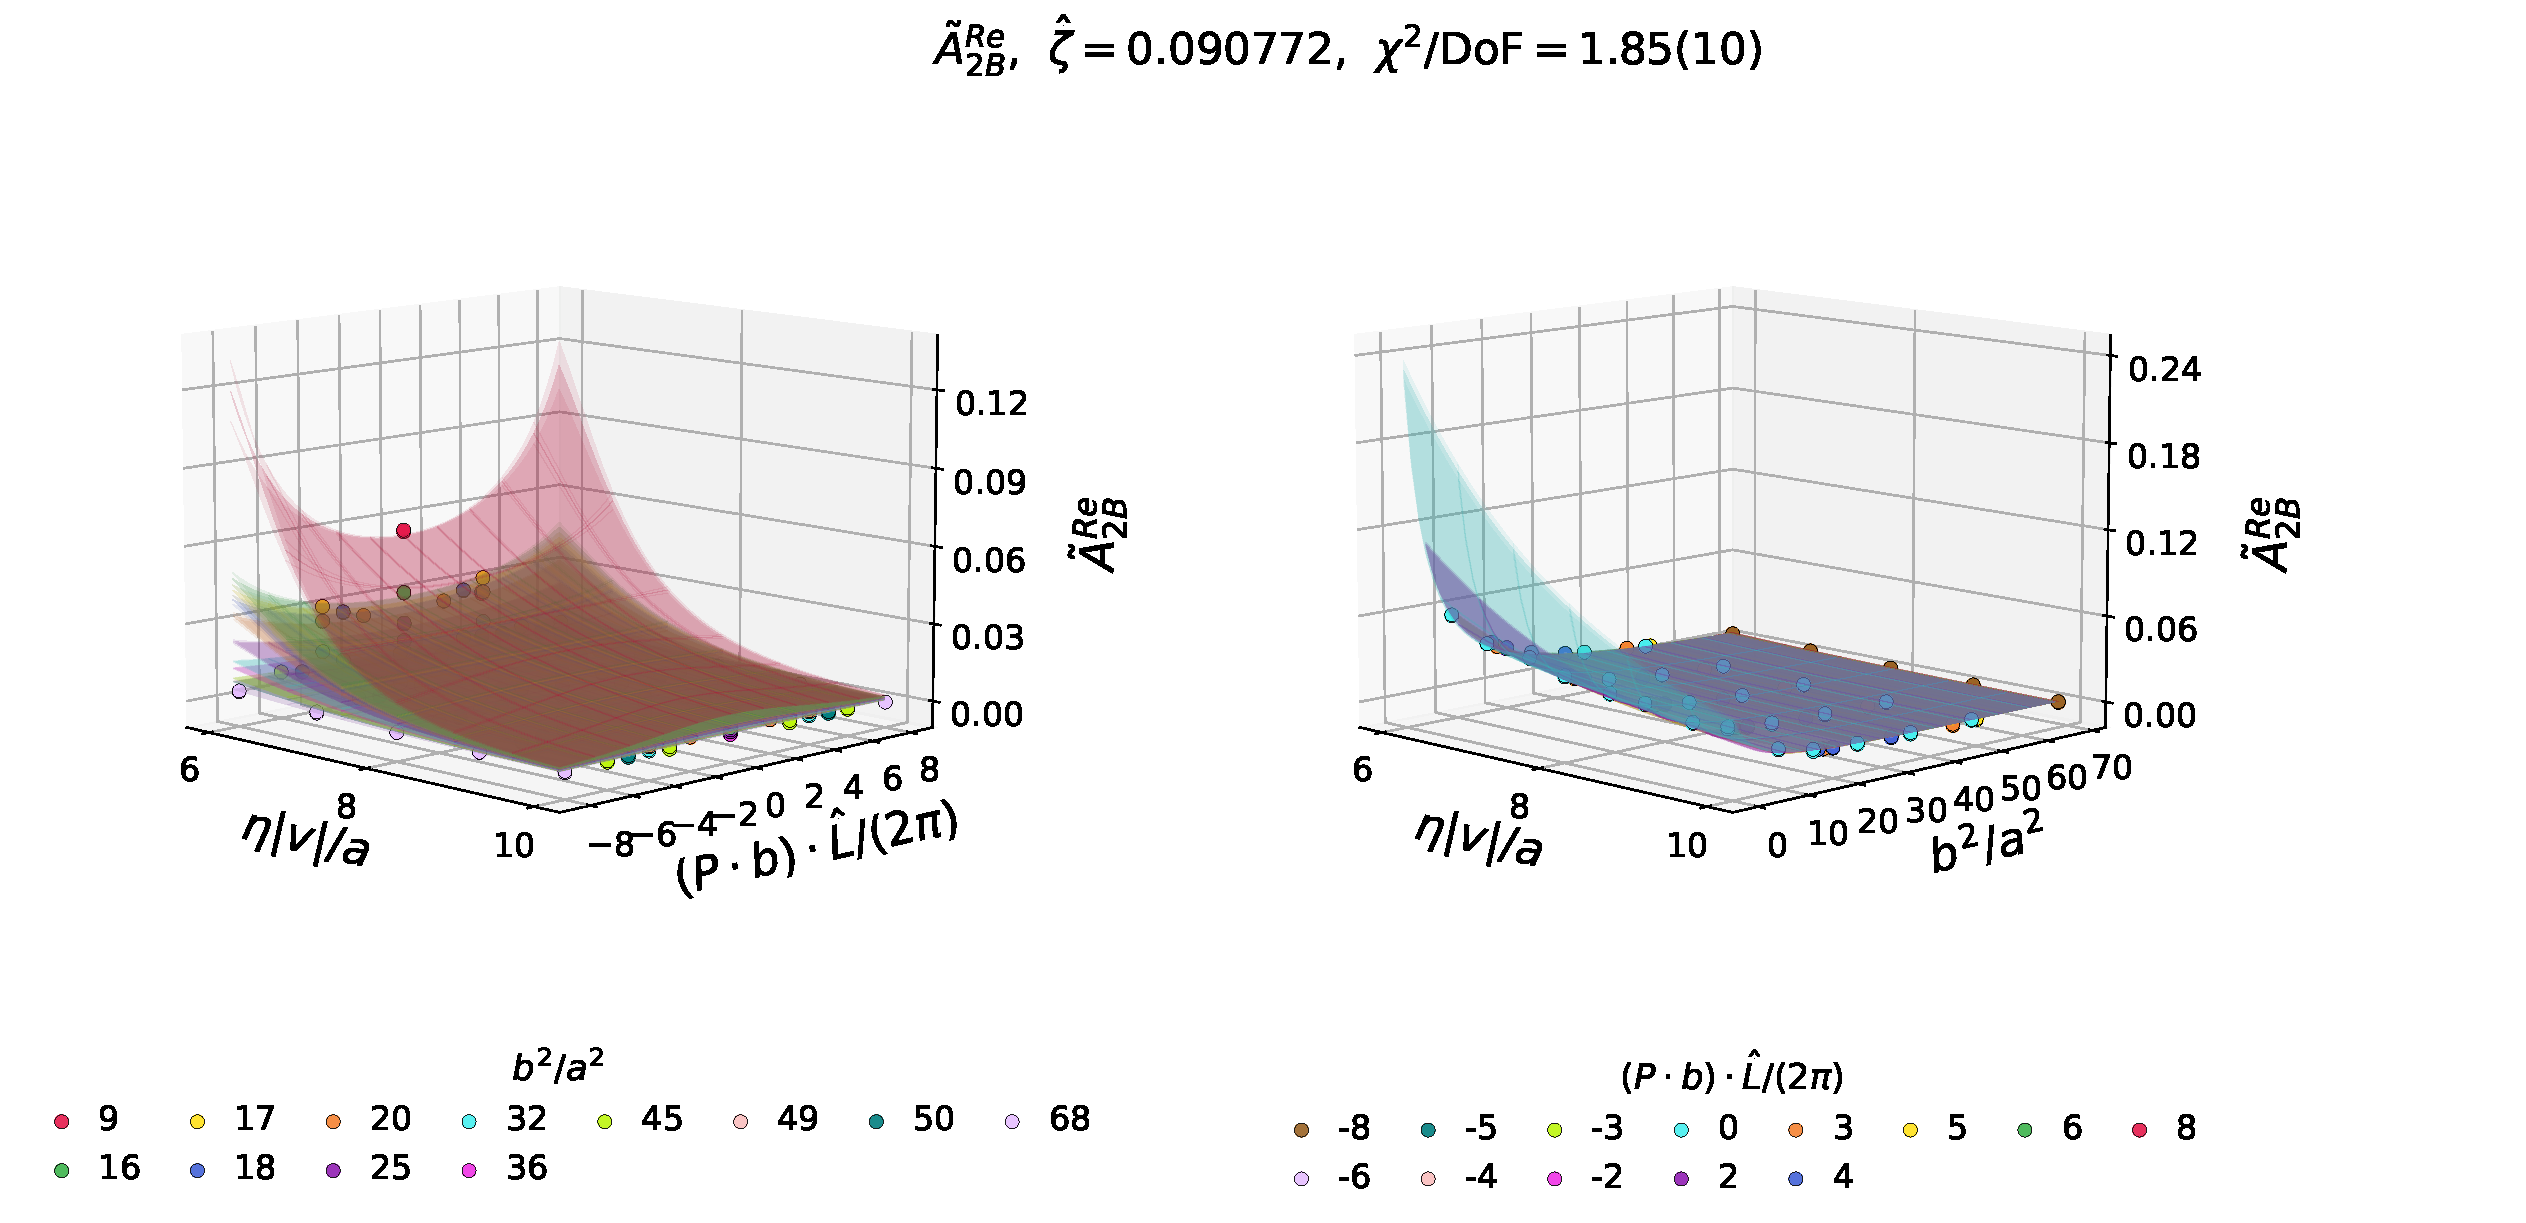
\includegraphics[width=\linewidth,height=.70\textheight,keepaspectratio]{fitting/ReA2B_Pb_bsq_PL-1_WithFit_3D.pdf}
\par\small Invariant coordinates: $(\nu,b^2,\eta)$. All panels and data overlays retained.

\figsrc{Thesis: plots; ReA2B\_Pb\_bsq\_PL-1\_WithFit\_3D}
\end{frame}

\begin{frame}{Fixed staple $\eta=8$: $\tAmp_{2B}^{\mathrm{Re}}$, $P_L=-1$}
\centering
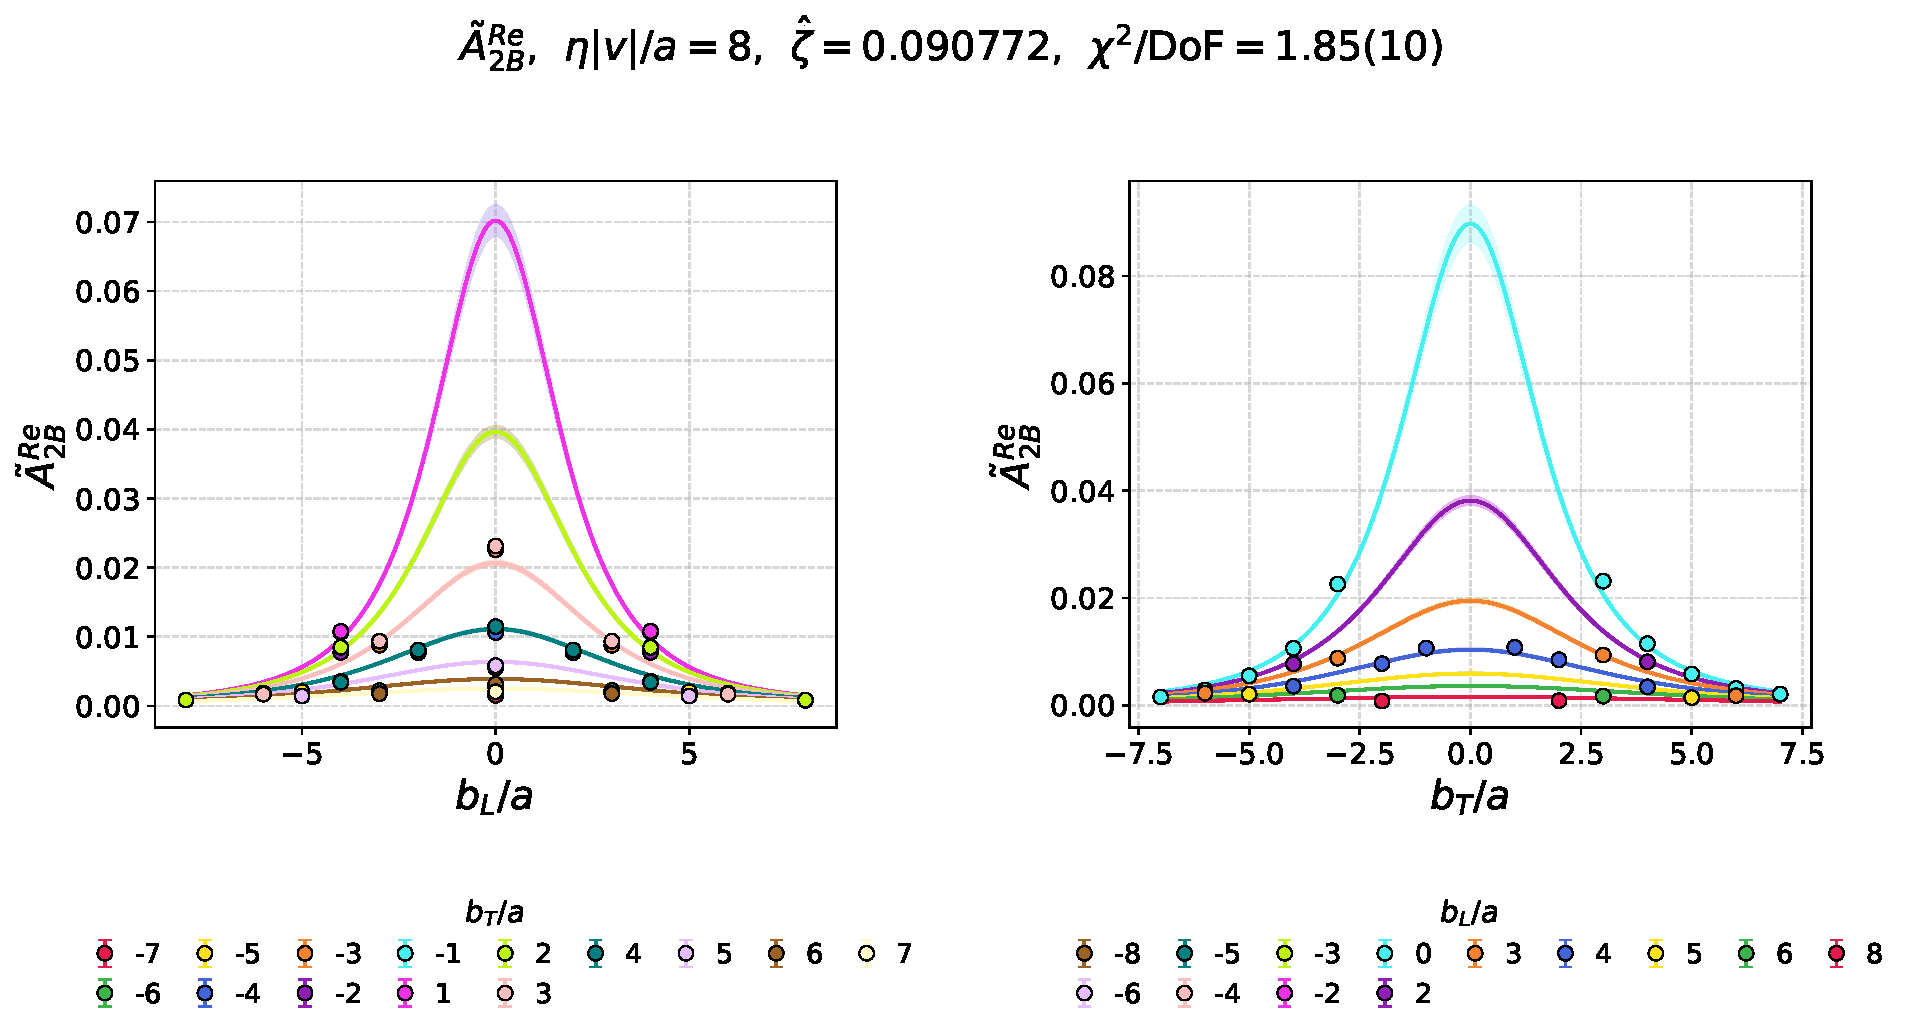
\includegraphics[width=\linewidth,height=.70\textheight,keepaspectratio]{fitting/ReA2B_eta8_PL-1_WithFit_2D.pdf}
\par\small Both spatial-coordinate slices. Same simultaneous fit, with Jackknife bands.

\figsrc{Thesis: plots; ReA2B\_eta8\_PL-1\_WithFit\_2D}
\end{frame}

\begin{frame}{Fixed staple $\eta=8$: $\tAmp_{2B}^{\mathrm{Re}}$, $P_L=-1$}
\centering
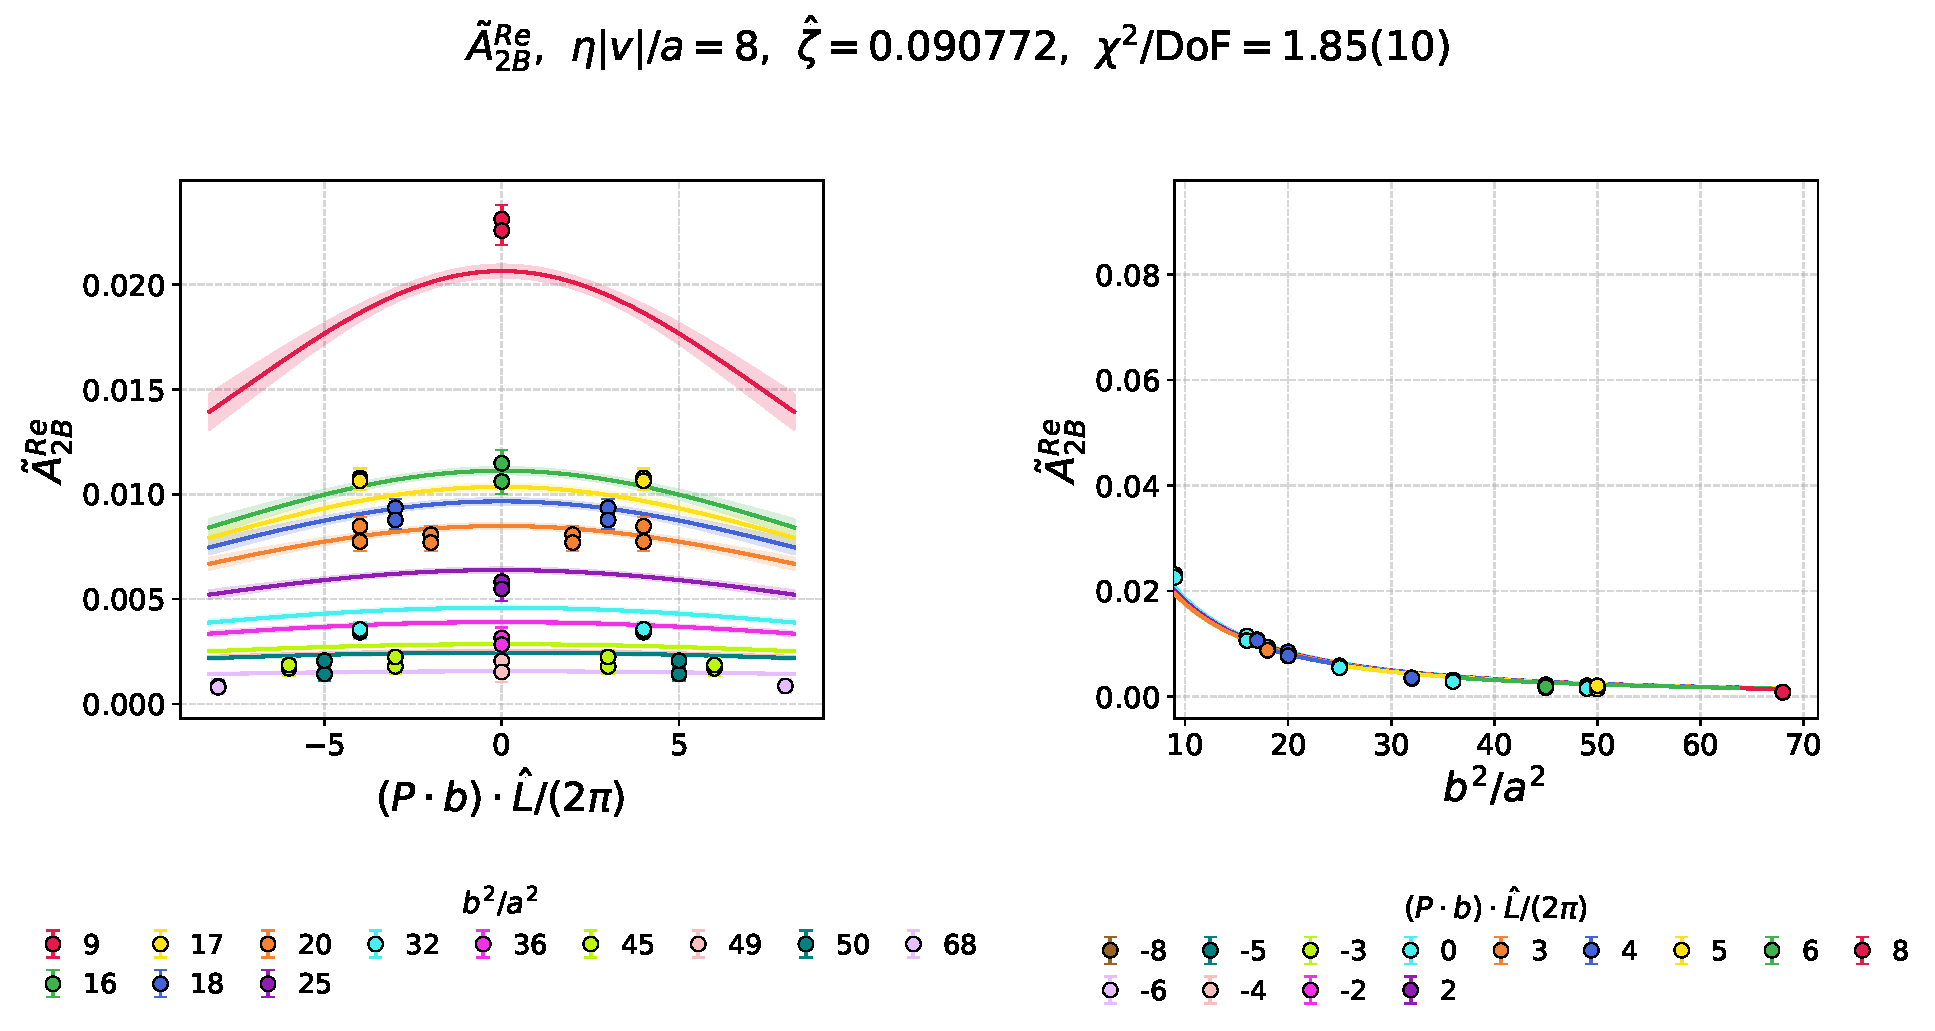
\includegraphics[width=\linewidth,height=.70\textheight,keepaspectratio]{fitting/ReA2B_Pb_bsq_eta8_PL-1_WithFit_2D.pdf}
\par\small Both invariant-coordinate slices. Same simultaneous fit, with Jackknife bands.

\figsrc{Thesis: plots; ReA2B\_Pb\_bsq\_eta8\_PL-1\_WithFit\_2D}
\end{frame}

\begin{frame}{Global fit: $\tAmp_{2B}^{\mathrm{Im}}$, $P_L=-1$}
\centering
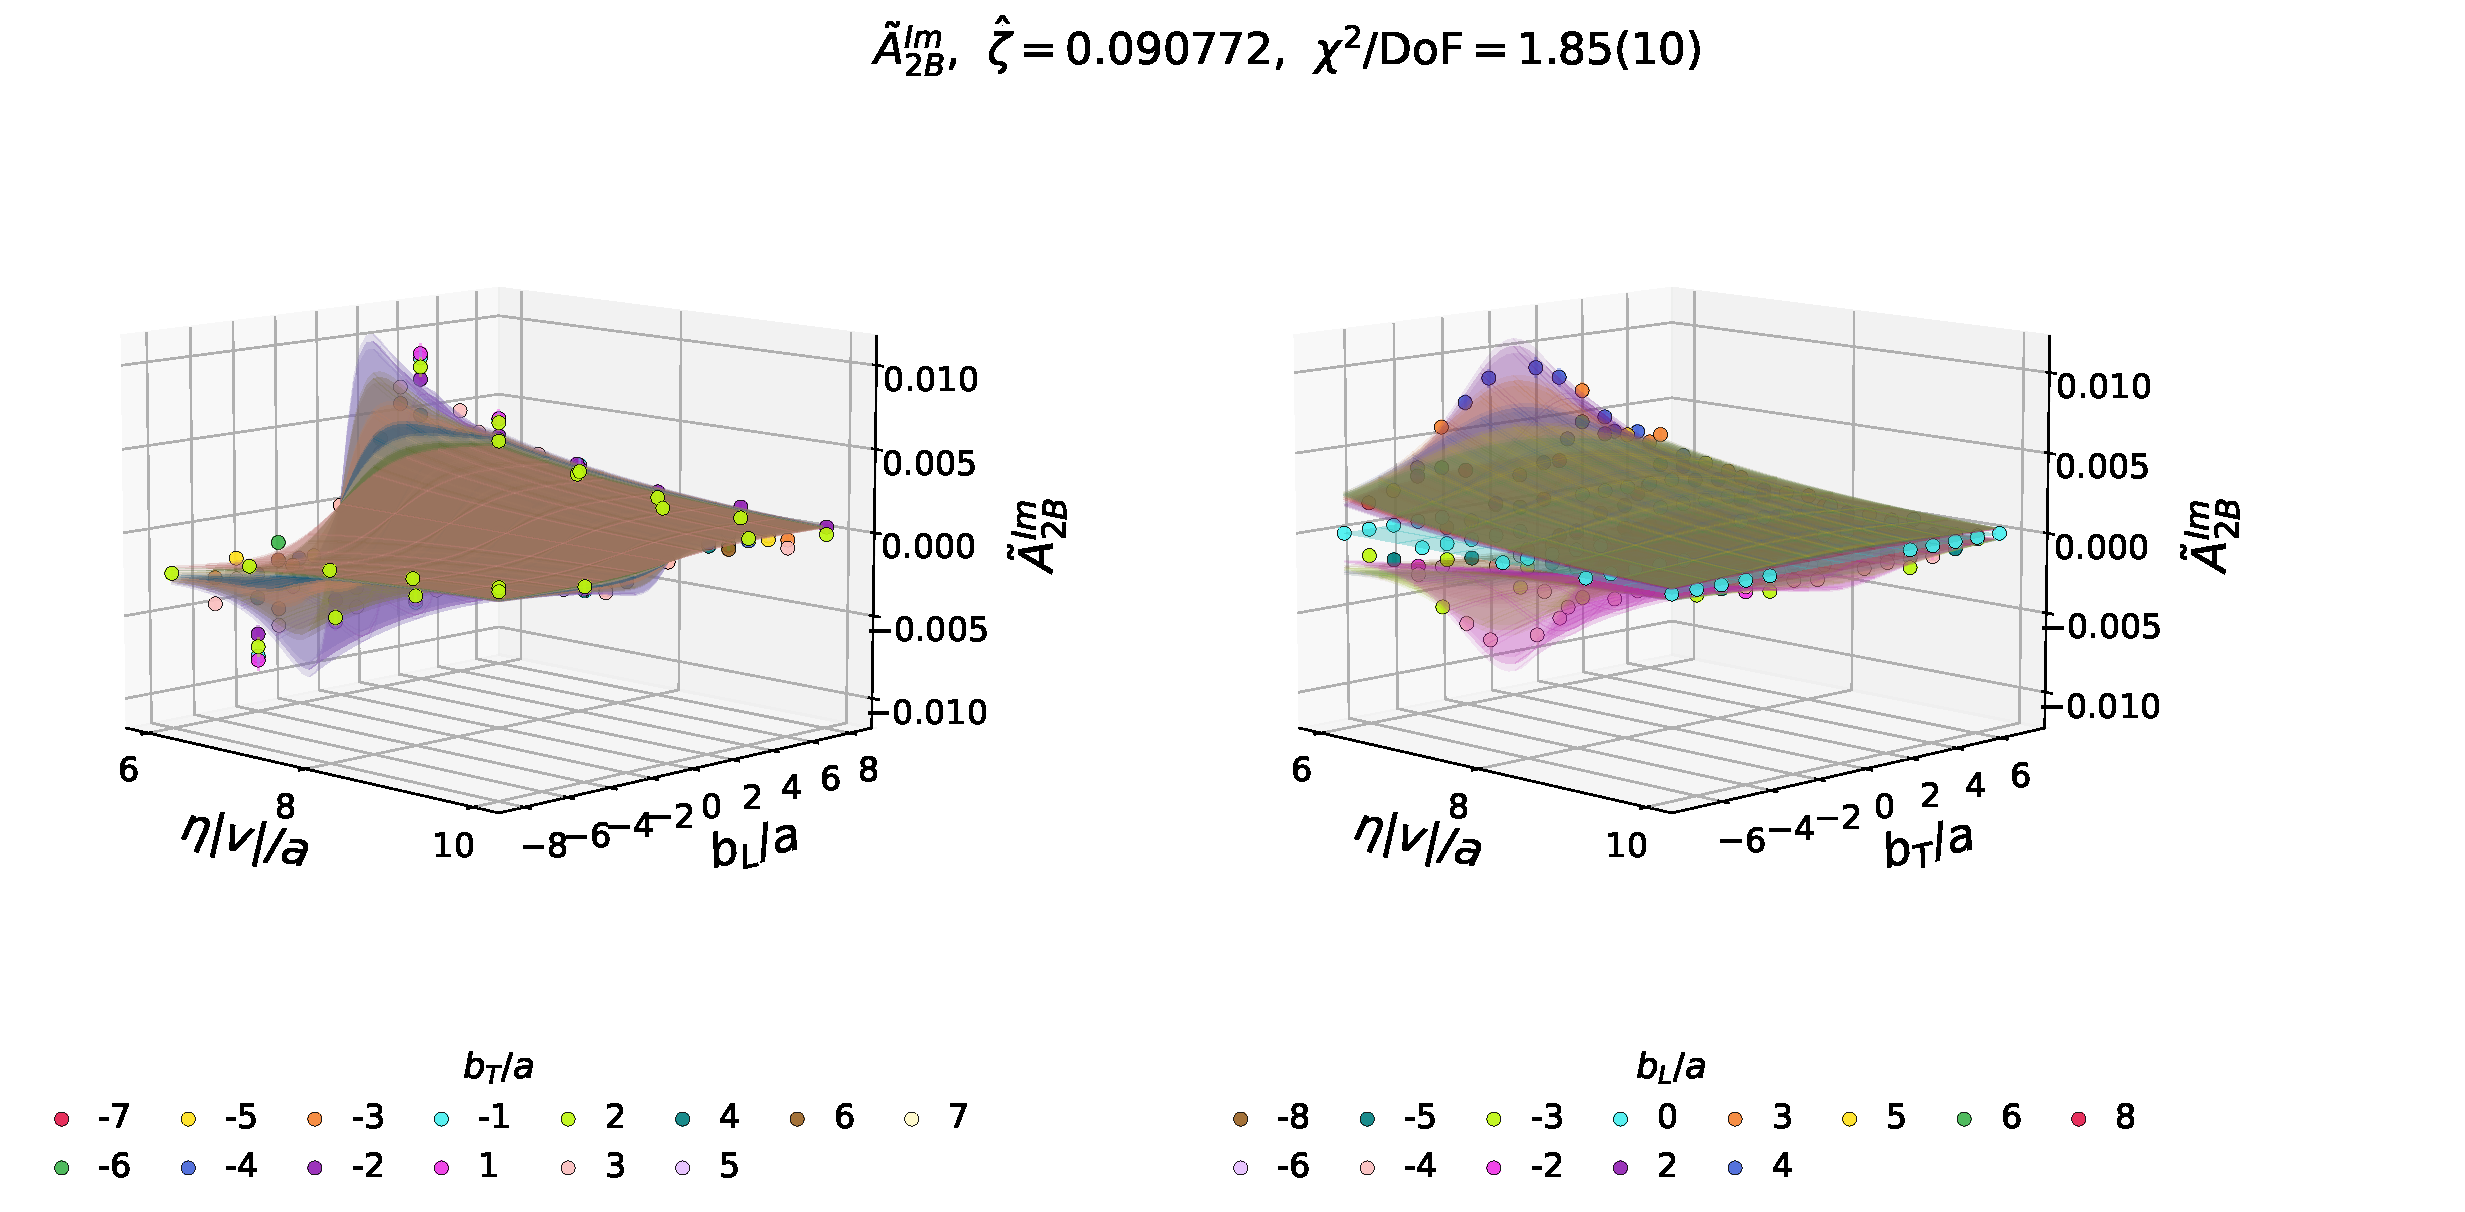
\includegraphics[width=\linewidth,height=.70\textheight,keepaspectratio]{fitting/ImA2B_PL-1_WithFit_3D.pdf}
\par\small Spatial coordinates: $(b_L,b_T,\eta)$. All panels and data overlays retained.

\figsrc{Thesis: plots; ImA2B\_PL-1\_WithFit\_3D}
\end{frame}

\begin{frame}{Global fit: $\tAmp_{2B}^{\mathrm{Im}}$, $P_L=-1$}
\centering
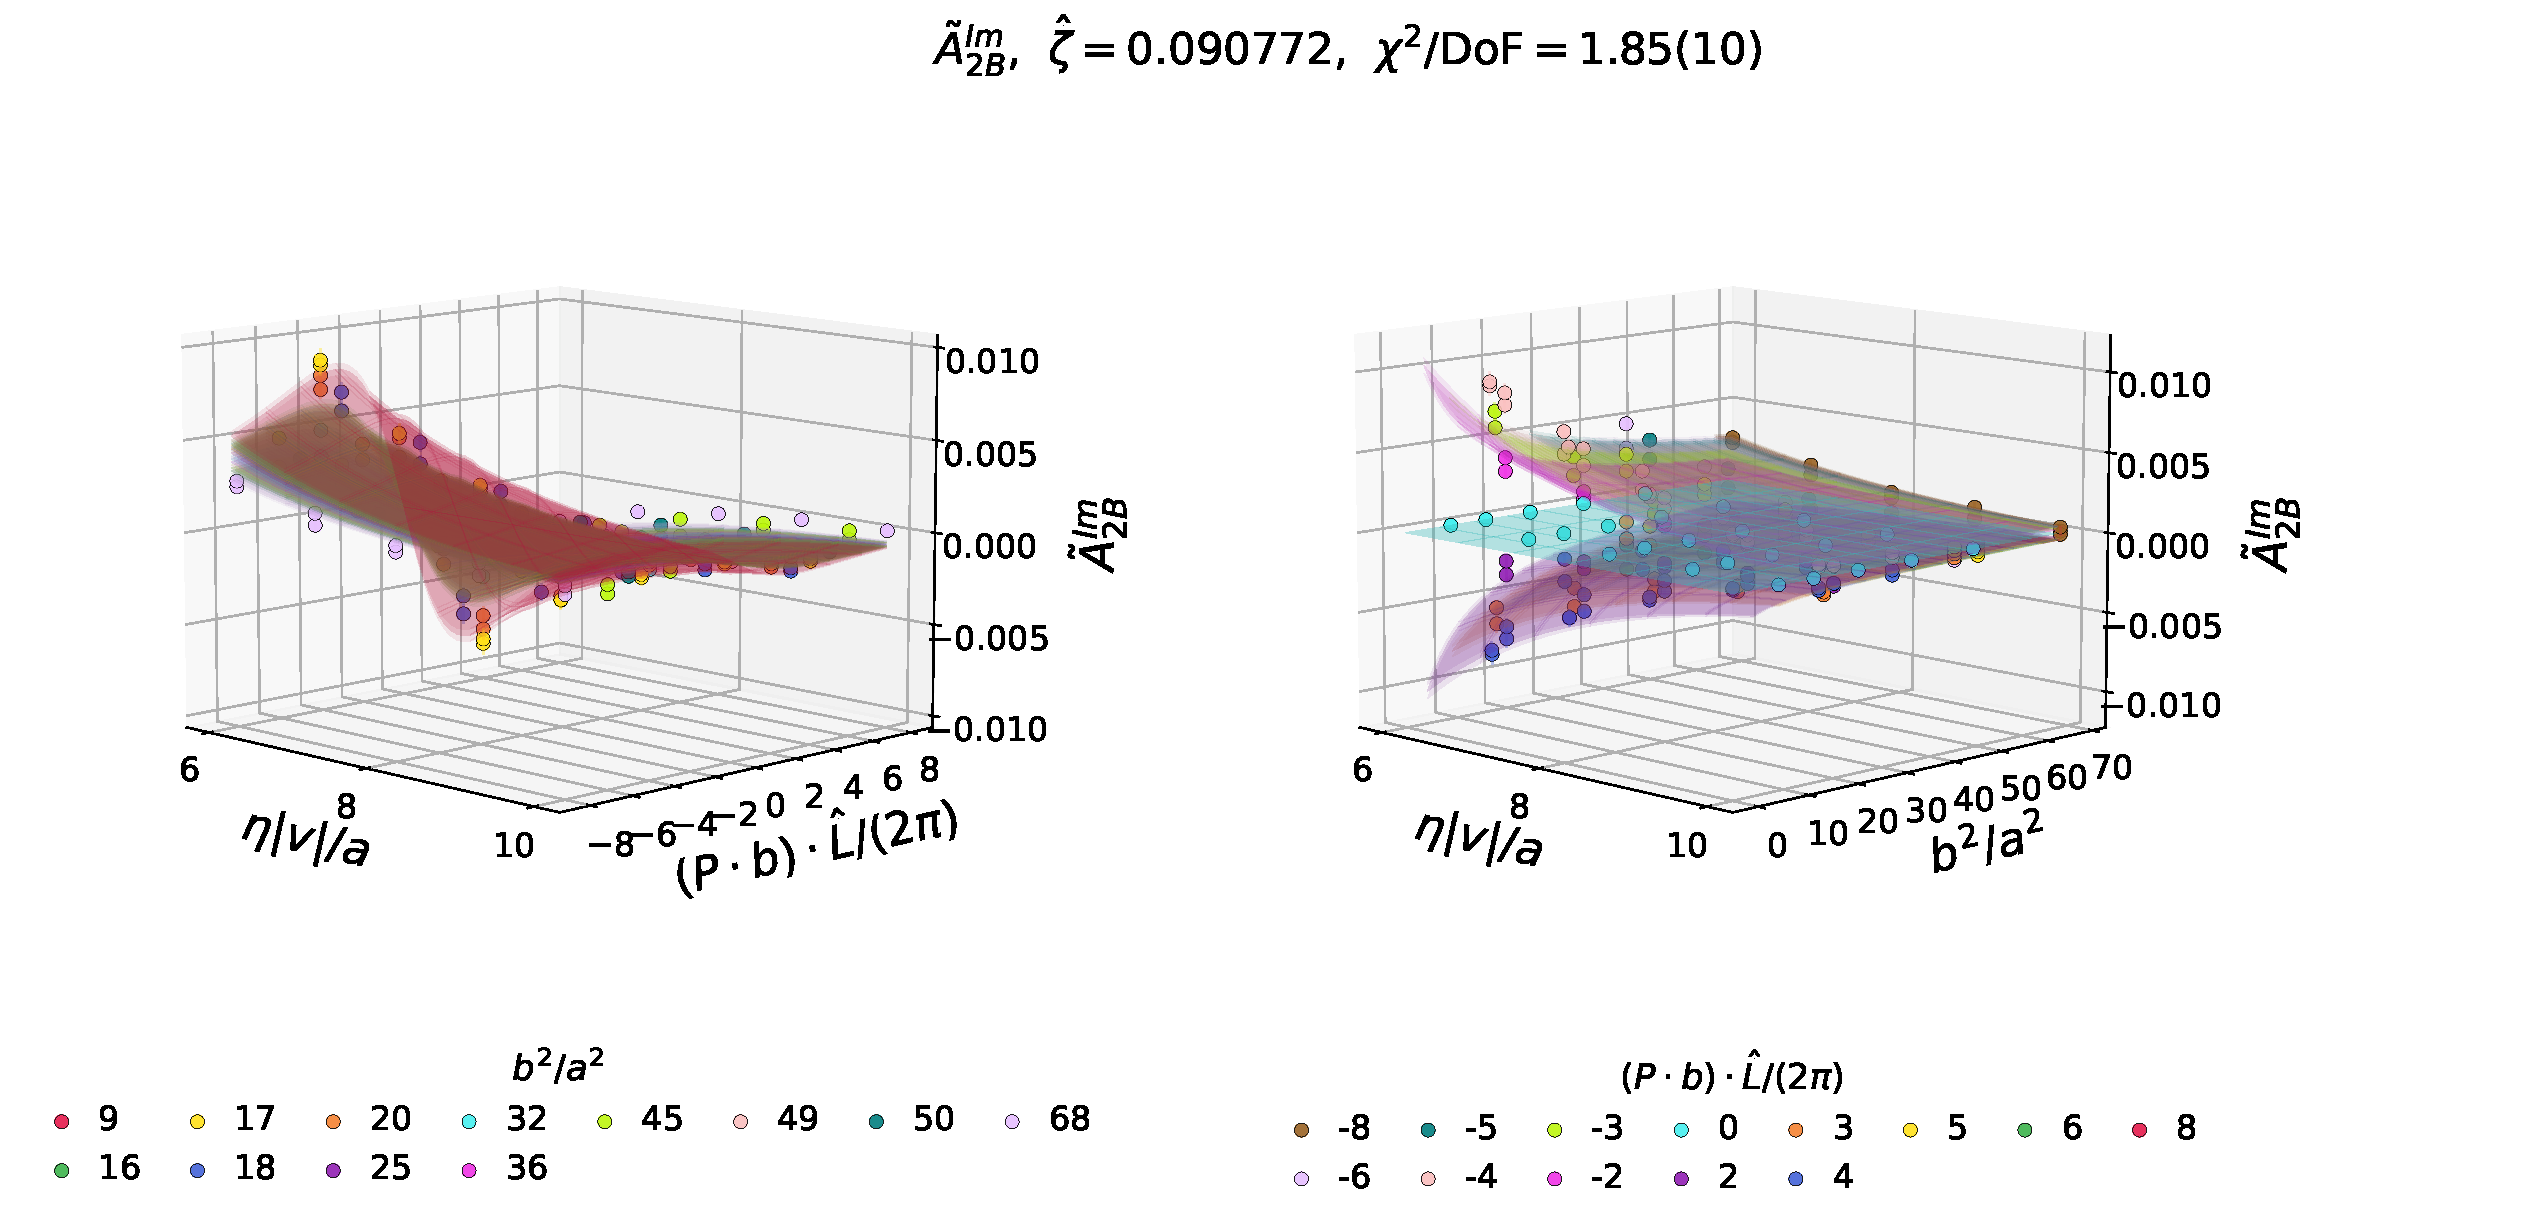
\includegraphics[width=\linewidth,height=.70\textheight,keepaspectratio]{fitting/ImA2B_Pb_bsq_PL-1_WithFit_3D.pdf}
\par\small Invariant coordinates: $(\nu,b^2,\eta)$. All panels and data overlays retained.

\figsrc{Thesis: plots; ImA2B\_Pb\_bsq\_PL-1\_WithFit\_3D}
\end{frame}

\begin{frame}{Fixed staple $\eta=8$: $\tAmp_{2B}^{\mathrm{Im}}$, $P_L=-1$}
\centering
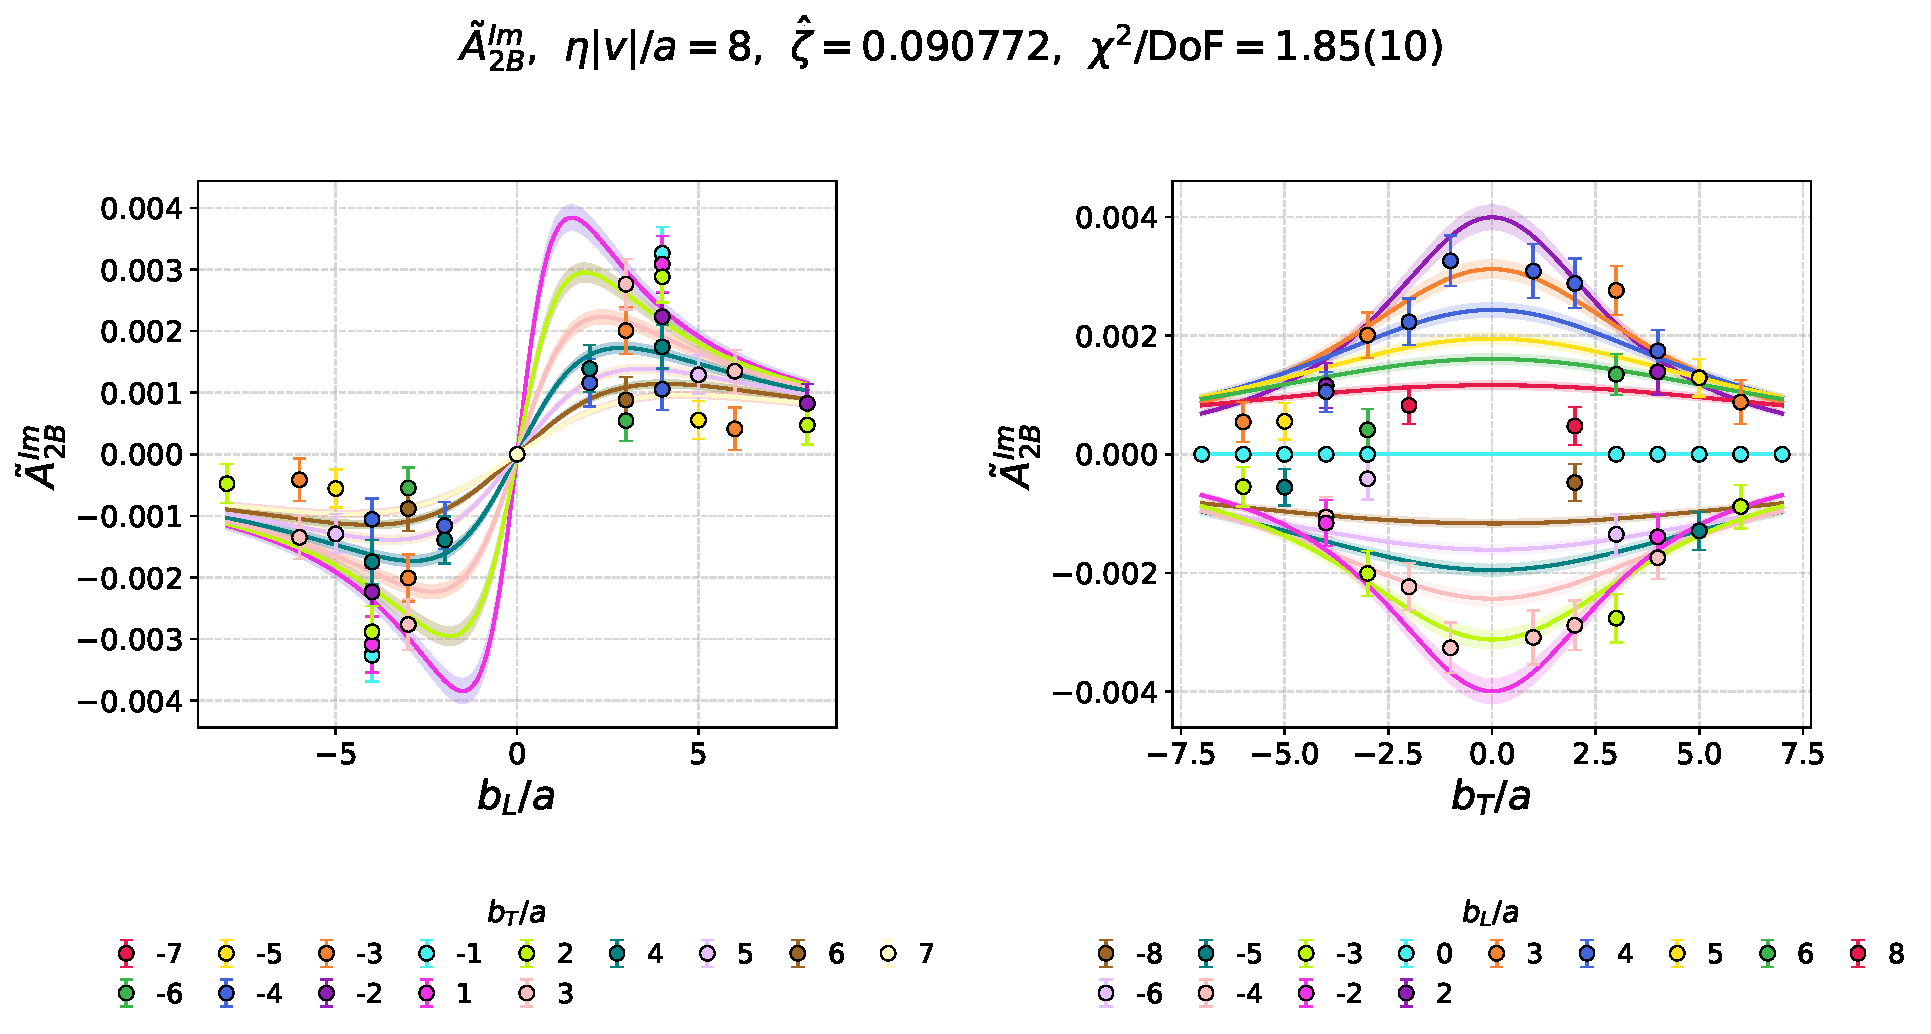
\includegraphics[width=\linewidth,height=.70\textheight,keepaspectratio]{fitting/ImA2B_eta8_PL-1_WithFit_2D.pdf}
\par\small Both spatial-coordinate slices. Same simultaneous fit, with Jackknife bands.

\figsrc{Thesis: plots; ImA2B\_eta8\_PL-1\_WithFit\_2D}
\end{frame}

\begin{frame}{Fixed staple $\eta=8$: $\tAmp_{2B}^{\mathrm{Im}}$, $P_L=-1$}
\centering
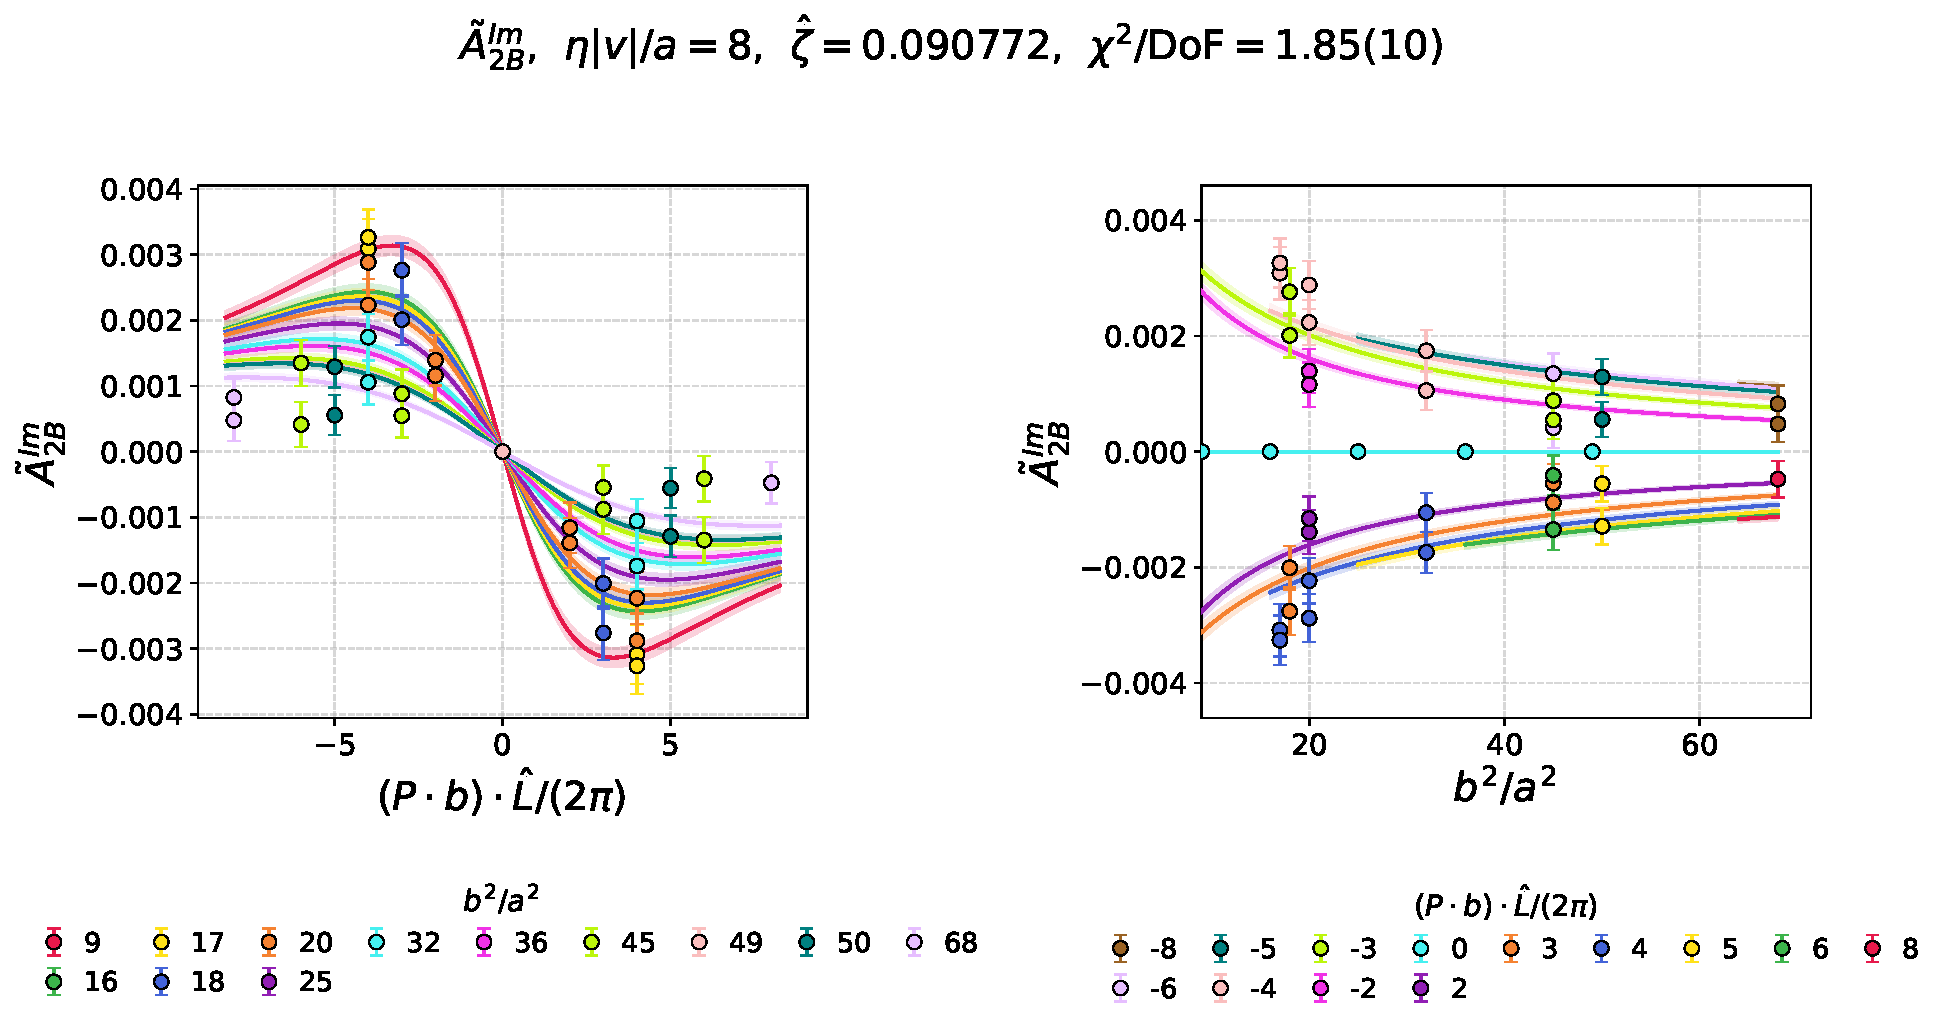
\includegraphics[width=\linewidth,height=.70\textheight,keepaspectratio]{fitting/ImA2B_Pb_bsq_eta8_PL-1_WithFit_2D.pdf}
\par\small Both invariant-coordinate slices. Same simultaneous fit, with Jackknife bands.

\figsrc{Thesis: plots; ImA2B\_Pb\_bsq\_eta8\_PL-1\_WithFit\_2D}
\end{frame}

\begin{frame}{Global fit: $\tAmp_{12B}^{\mathrm{Re}}$, $P_L=-1$}
\centering
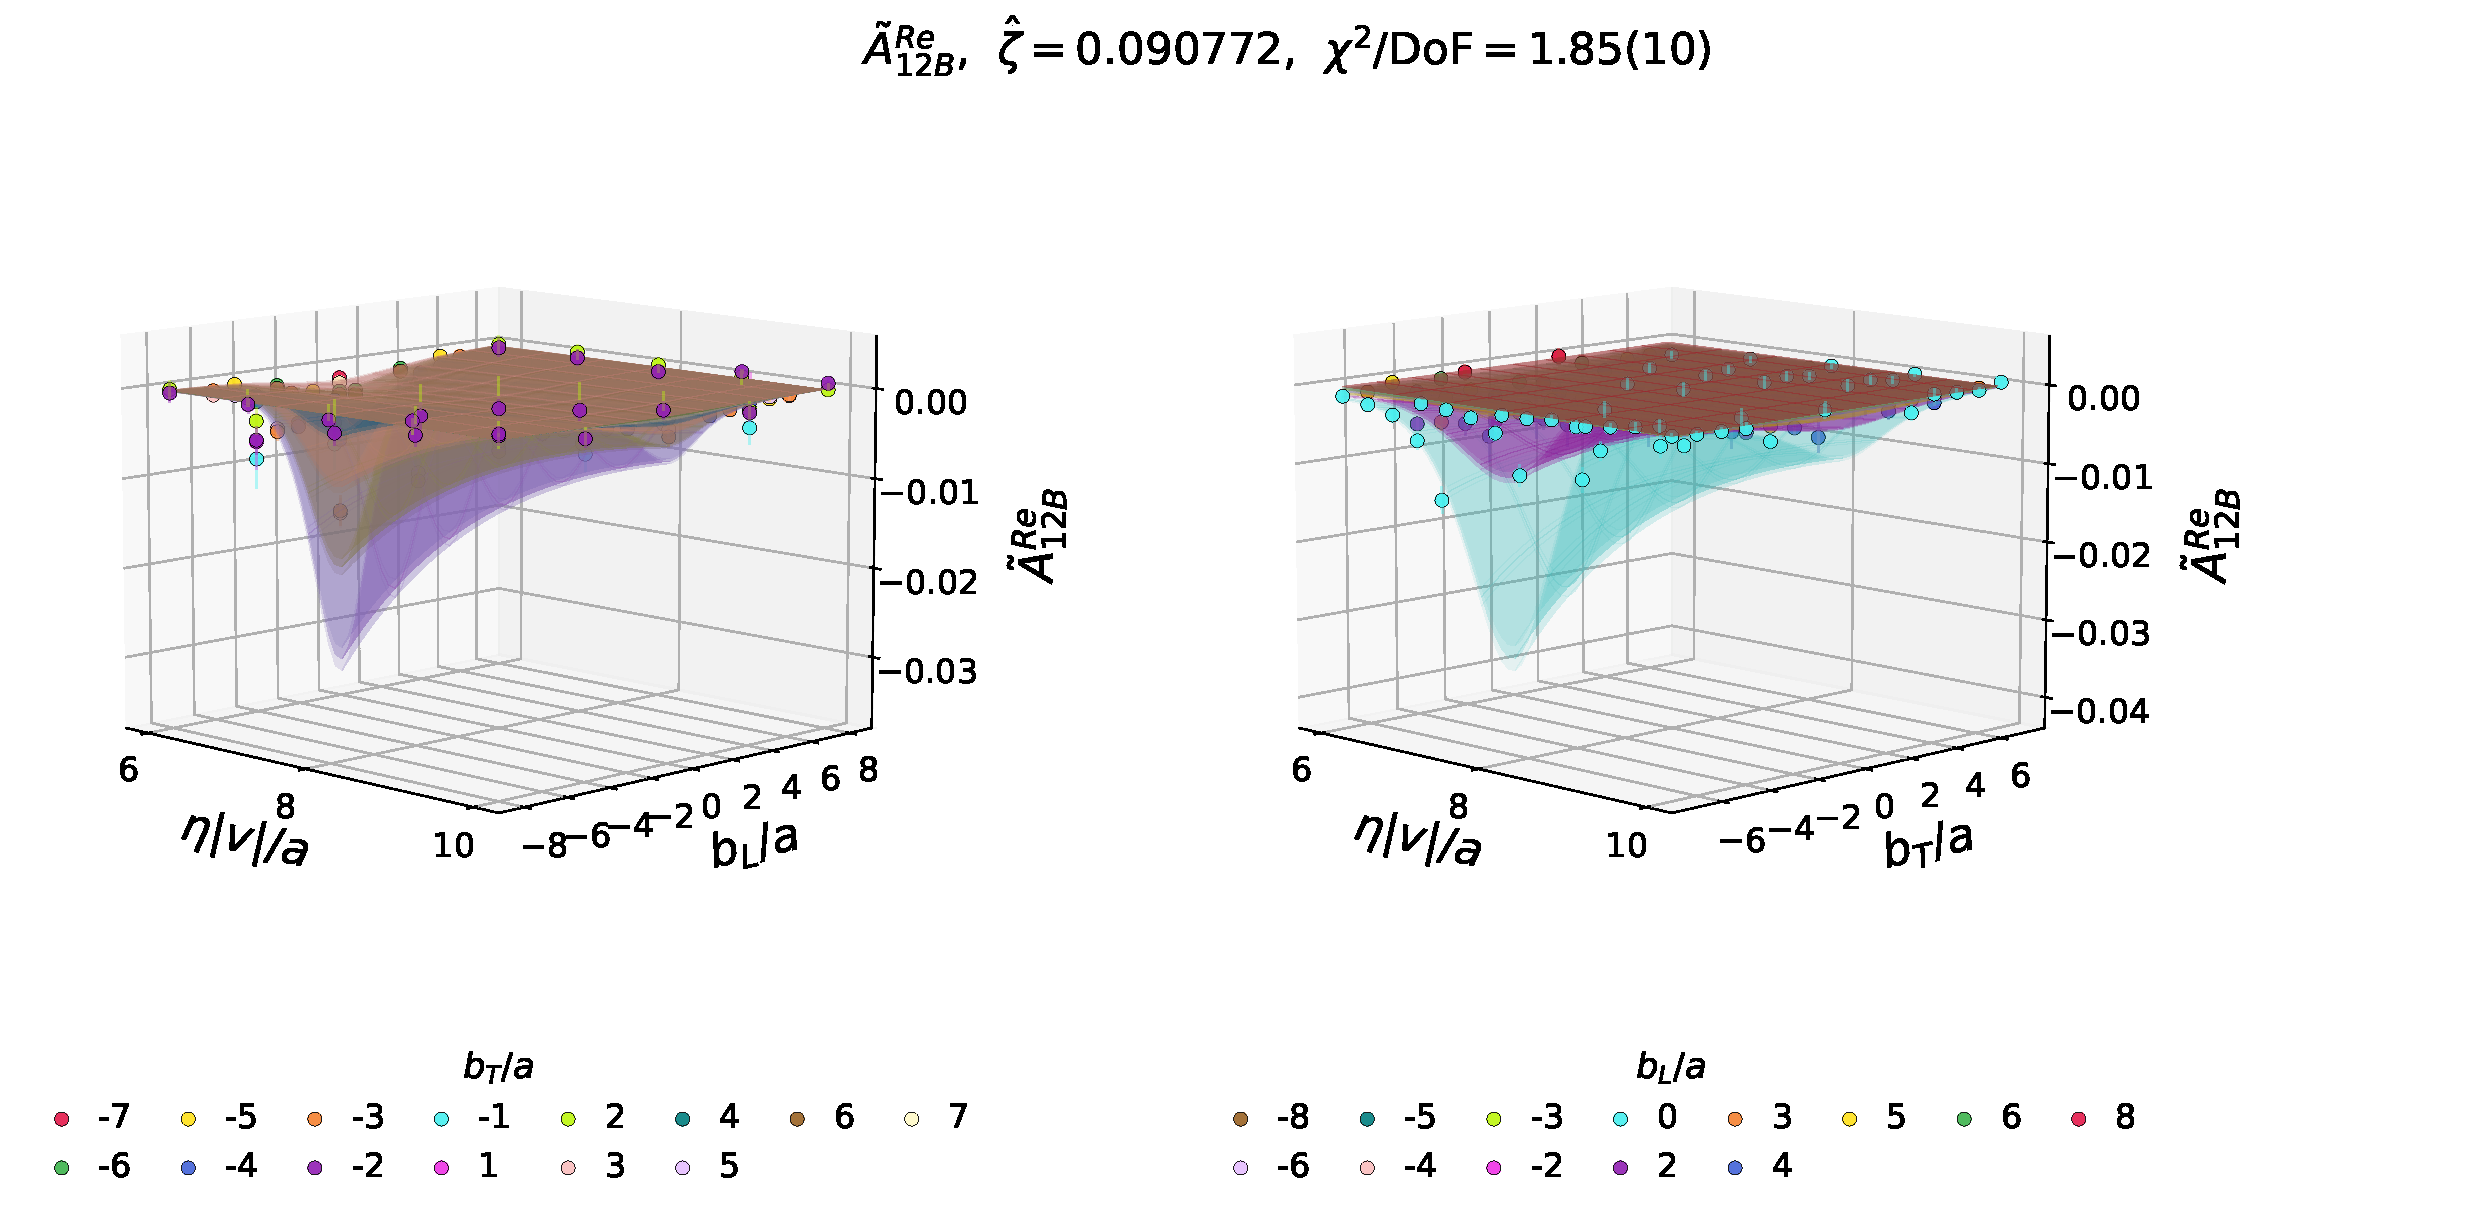
\includegraphics[width=\linewidth,height=.70\textheight,keepaspectratio]{fitting/ReA12B_PL-1_WithFit_3D.pdf}
\par\small Spatial coordinates: $(b_L,b_T,\eta)$. All panels and data overlays retained.

\figsrc{Thesis: plots; ReA12B\_PL-1\_WithFit\_3D}
\end{frame}

\begin{frame}{Global fit: $\tAmp_{12B}^{\mathrm{Re}}$, $P_L=-1$}
\centering
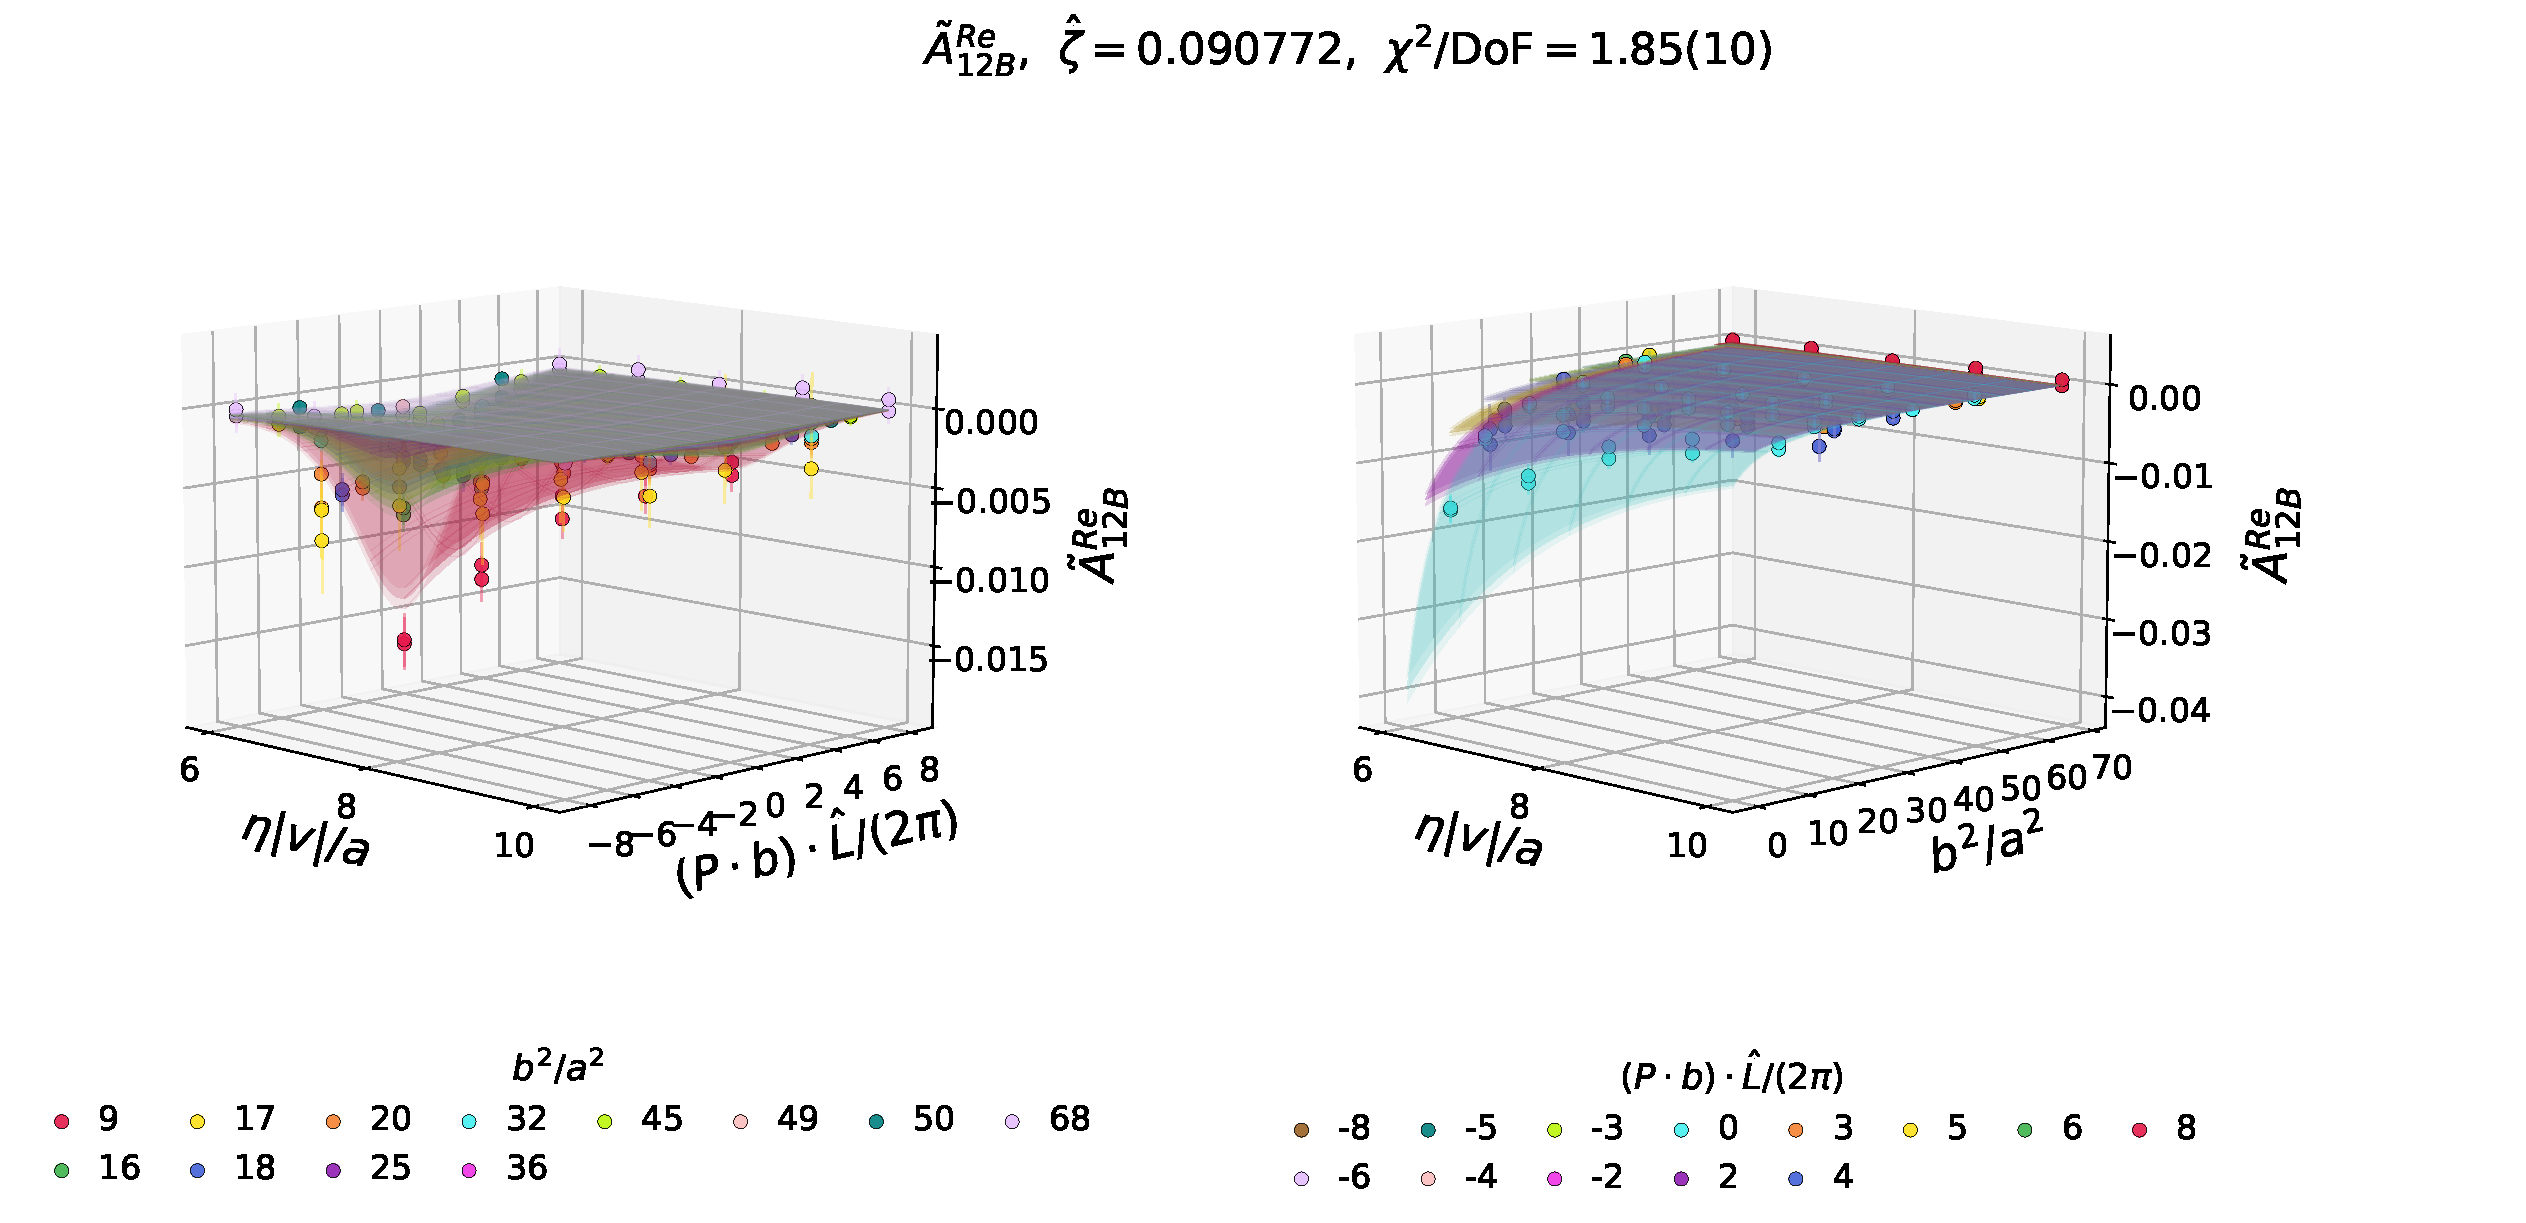
\includegraphics[width=\linewidth,height=.70\textheight,keepaspectratio]{fitting/ReA12B_Pb_bsq_PL-1_WithFit_3D.pdf}
\par\small Invariant coordinates: $(\nu,b^2,\eta)$. All panels and data overlays retained.

\figsrc{Thesis: plots; ReA12B\_Pb\_bsq\_PL-1\_WithFit\_3D}
\end{frame}

\begin{frame}{Fixed staple $\eta=8$: $\tAmp_{12B}^{\mathrm{Re}}$, $P_L=-1$}
\centering
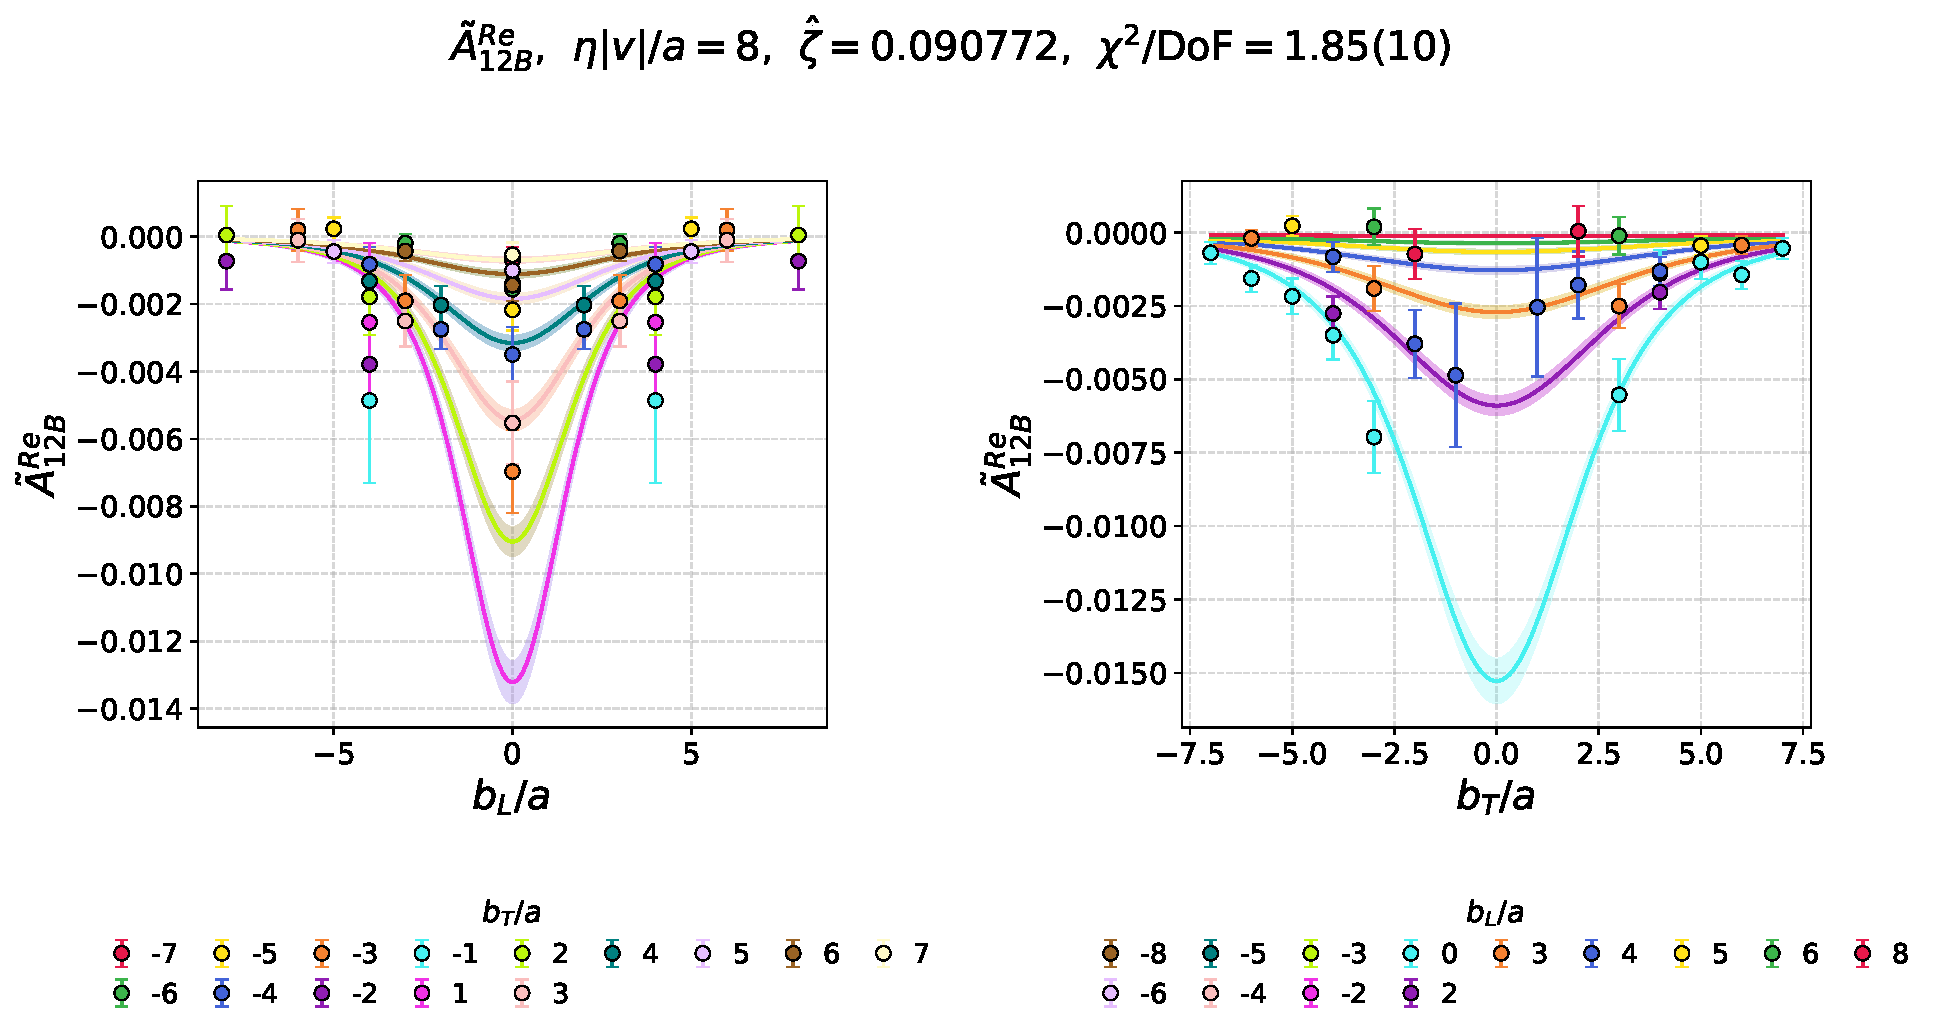
\includegraphics[width=\linewidth,height=.70\textheight,keepaspectratio]{fitting/ReA12B_eta8_PL-1_WithFit_2D.pdf}
\par\small Both spatial-coordinate slices. Same simultaneous fit, with Jackknife bands.

\figsrc{Thesis: plots; ReA12B\_eta8\_PL-1\_WithFit\_2D}
\end{frame}

\begin{frame}{Fixed staple $\eta=8$: $\tAmp_{12B}^{\mathrm{Re}}$, $P_L=-1$}
\centering
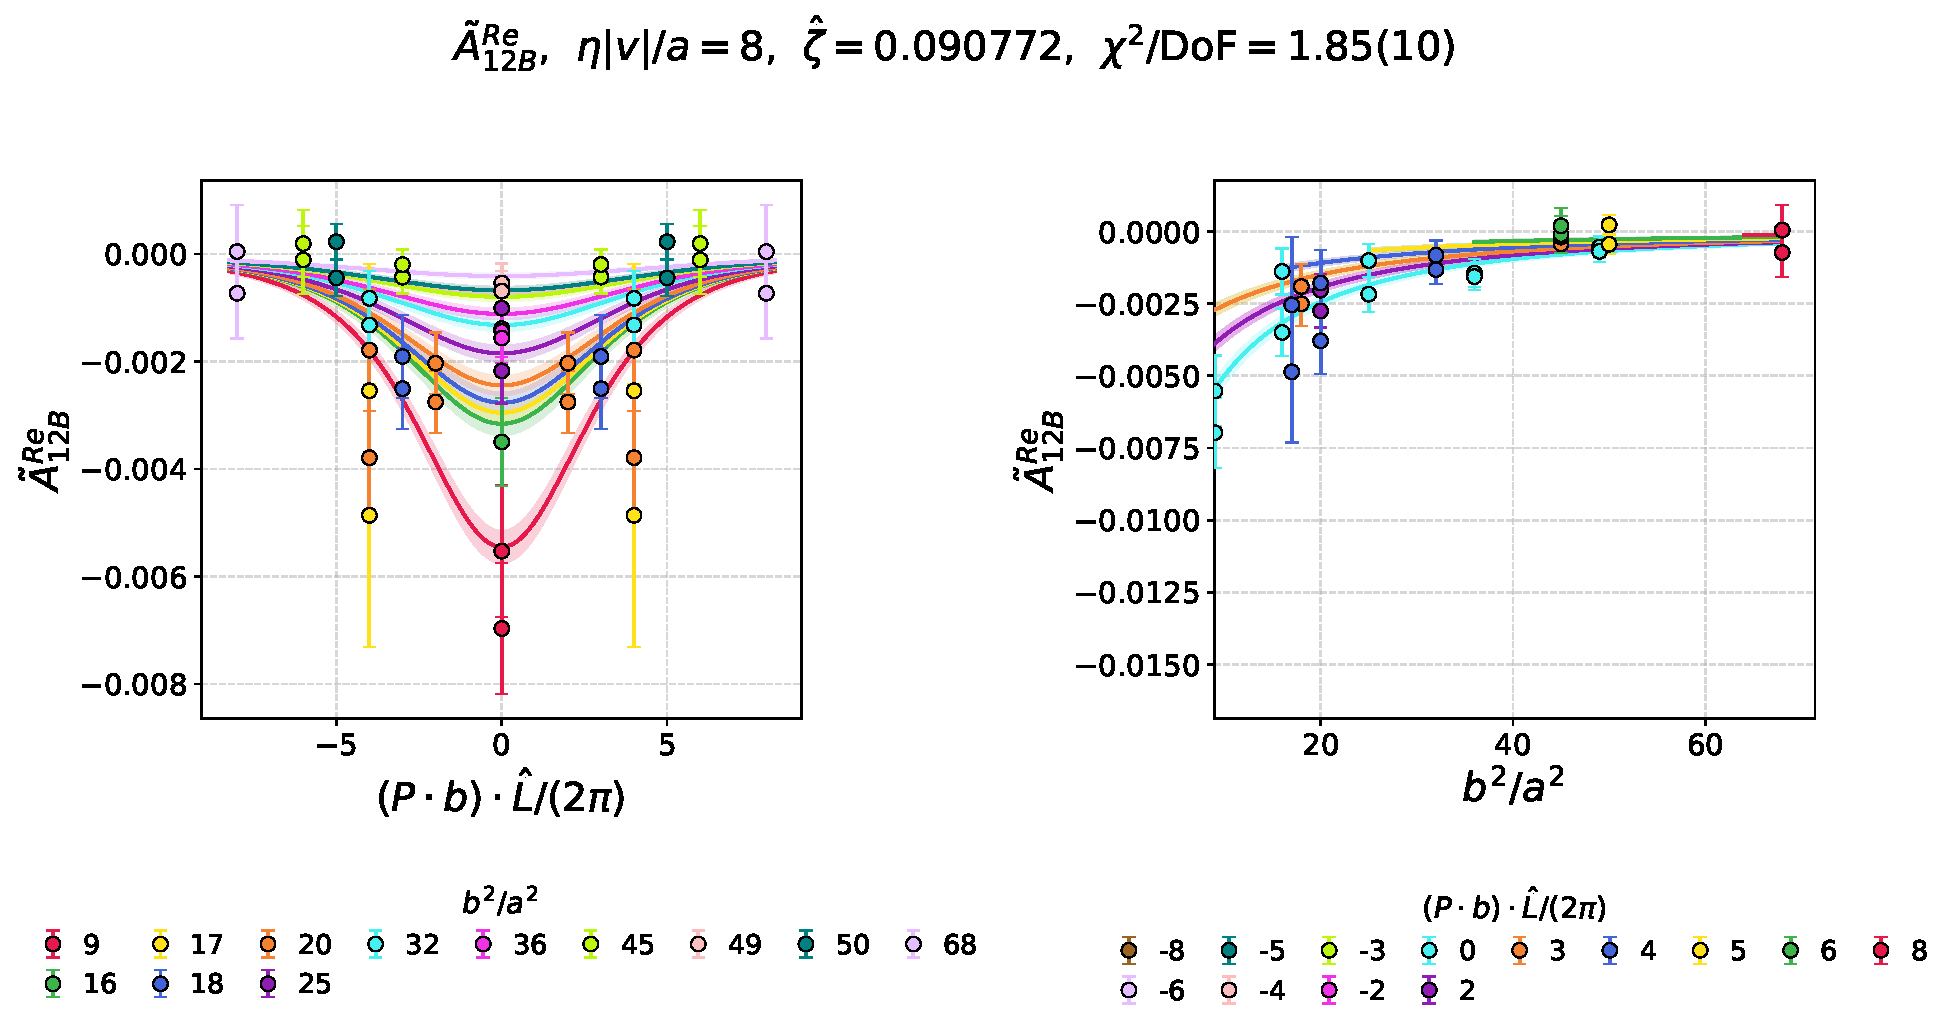
\includegraphics[width=\linewidth,height=.70\textheight,keepaspectratio]{fitting/ReA12B_Pb_bsq_eta8_PL-1_WithFit_2D.pdf}
\par\small Both invariant-coordinate slices. Same simultaneous fit, with Jackknife bands.

\figsrc{Thesis: plots; ReA12B\_Pb\_bsq\_eta8\_PL-1\_WithFit\_2D}
\end{frame}

\begin{frame}{Integrated Fourier results: $P_L=-1$}
\small\renewcommand{\arraystretch}{1.8}\begin{tabular}{lcccc}\toprule Integral & $(-\infty,\infty)$ & $[-1,1]$ & $[-1,0]$ & $[0,1]$\\\midrule
$\int dx\,E$ & 0.889(24) & 0.780(29) & 0.390(14) & 0.390(14) \\
$\int dx\,O$ & -1(108)e-17 & 2(282)e-17 & 0.1223(58) & -0.1223(58) \\
$\int dx\,\tilde f_1^{(0)}$ & 1.778(47) & 1.560(58) & 0.535(25) & 1.024(36) \\
$\int dx\,\tilde f_{1T}^{\perp(1)}$ & 0.469(23) & 0.454(23) & 0.227(12) & 0.227(12) \\
$m_N\int dx\,\tilde f_{1T}^{\perp(1)}/\int dx\,\tilde f_1^{(0)}$ & 0.284(14) & 0.313(18) & 0.456(29) & 0.238(13) \\
\bottomrule\end{tabular}\par\medskip $b^2=9a^2$; all values and Jackknife uncertainties retained. Numerical values retain the source normalization. The last row is in GeV.
\figsrc{Thesis: SimultaneousFitsCov/Integration\_Table\_PL-1\_bmin3\_b2-9.tex}
\end{frame}

\begin{frame}{Fourier results (2D): $P_L=-1$, unpolarized}
\centering
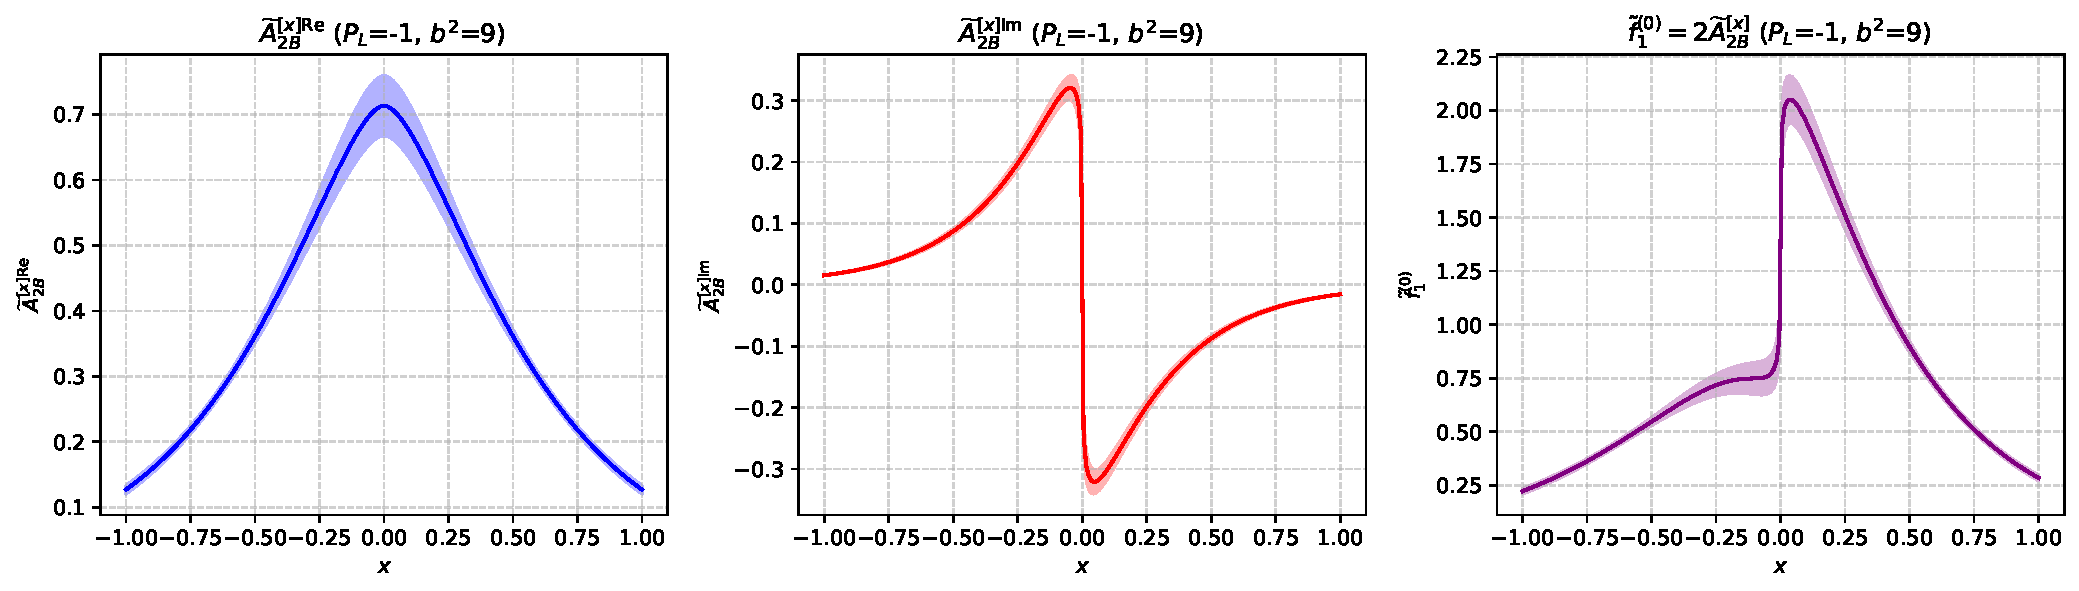
\includegraphics[width=\linewidth,height=.70\textheight,keepaspectratio]{fitting/FT_xdep_A2B_A12B_bmin3_eta610_b2-9_PL-1__row1.pdf}
\par\small Even, odd, and unpolarized transforms. Fixed $b^2=9a^2$.

\figsrc{Thesis: SimultaneousFitsCov; FT\_xdep\_A2B\_A12B\_bmin3\_eta610\_b2-9\_PL-1}
\end{frame}

\begin{frame}{Fourier results (2D): $P_L=-1$, Sivers}
\centering
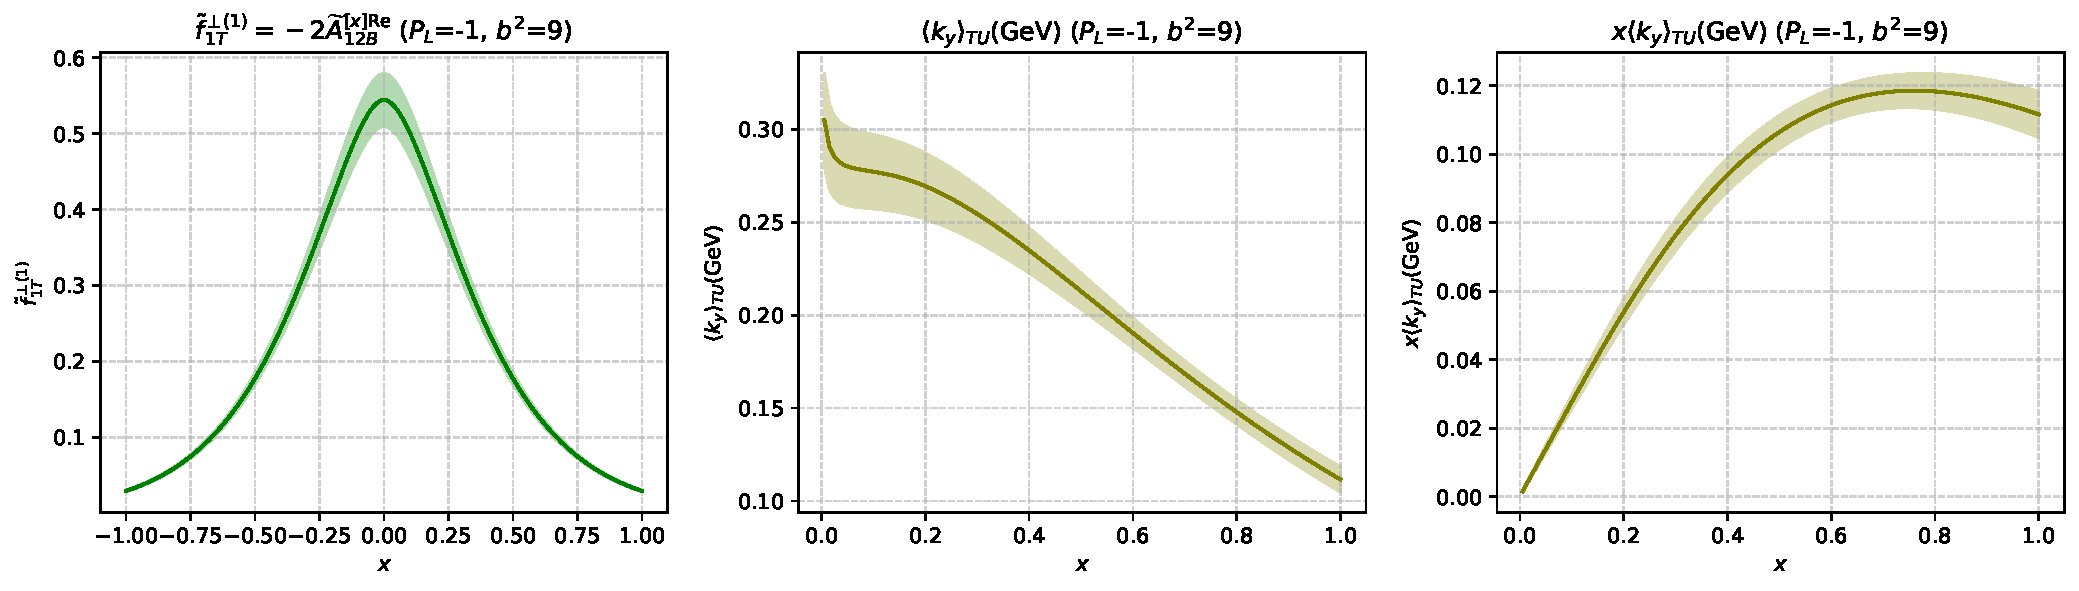
\includegraphics[width=\linewidth,height=.70\textheight,keepaspectratio]{fitting/FT_xdep_A2B_A12B_bmin3_eta610_b2-9_PL-1__row2.pdf}
\par\small Sivers transform, shift, and $x\langle k_y\rangle_{TU}$. Fixed $b^2=9a^2$.

\figsrc{Thesis: SimultaneousFitsCov; FT\_xdep\_A2B\_A12B\_bmin3\_eta610\_b2-9\_PL-1}
\end{frame}

\begin{frame}{Fourier results (3D): $P_L=-1$, unpolarized}
\centering
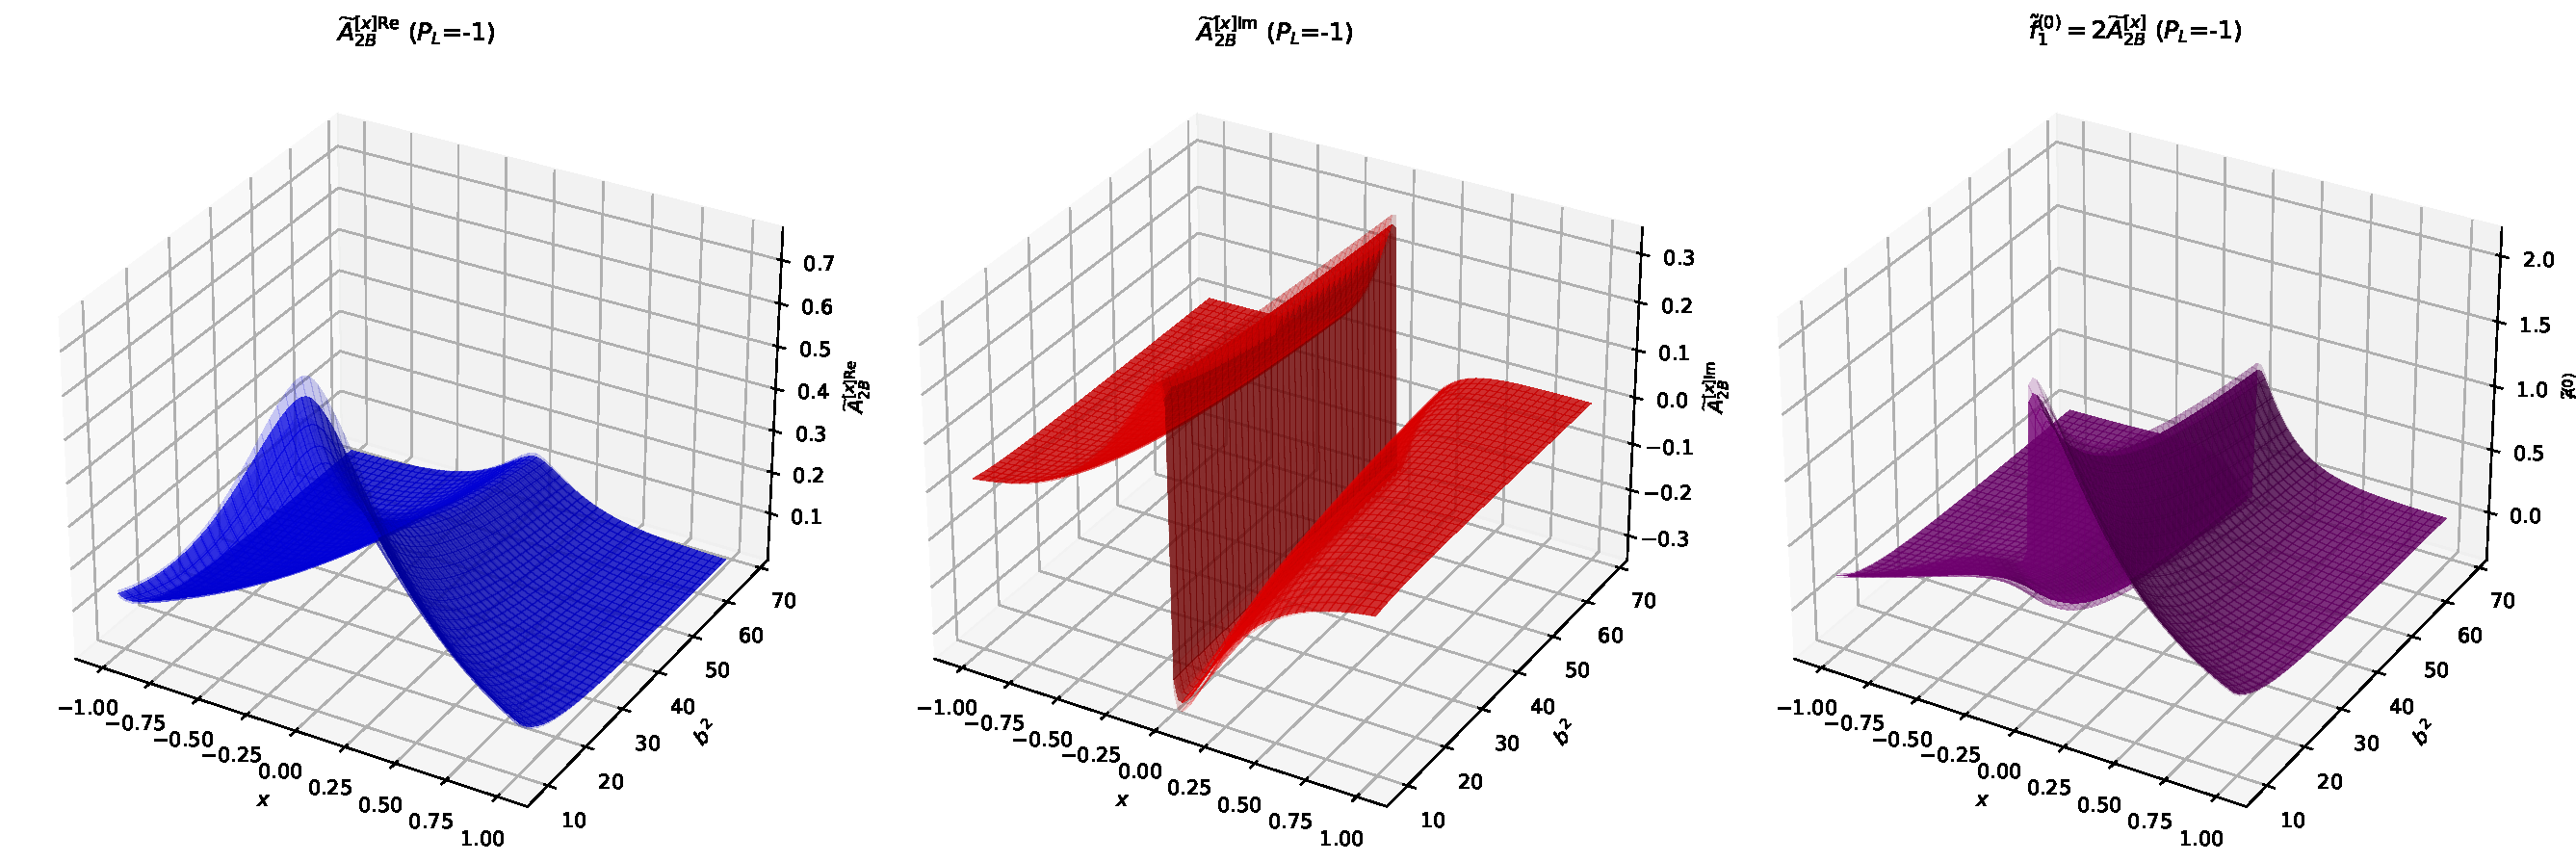
\includegraphics[width=\linewidth,height=.70\textheight,keepaspectratio]{fitting/FT_xdep_3D_A2B_A12B_bmin3_eta610_PL-1__row1.pdf}
\par\small Even, odd, and unpolarized transforms. Full $b^2/a^2\in[9,68]$ dependence.

\figsrc{Thesis: SimultaneousFitsCov; FT\_xdep\_3D\_A2B\_A12B\_bmin3\_eta610\_PL-1}
\end{frame}

\begin{frame}{Fourier results (3D): $P_L=-1$, Sivers}
\centering
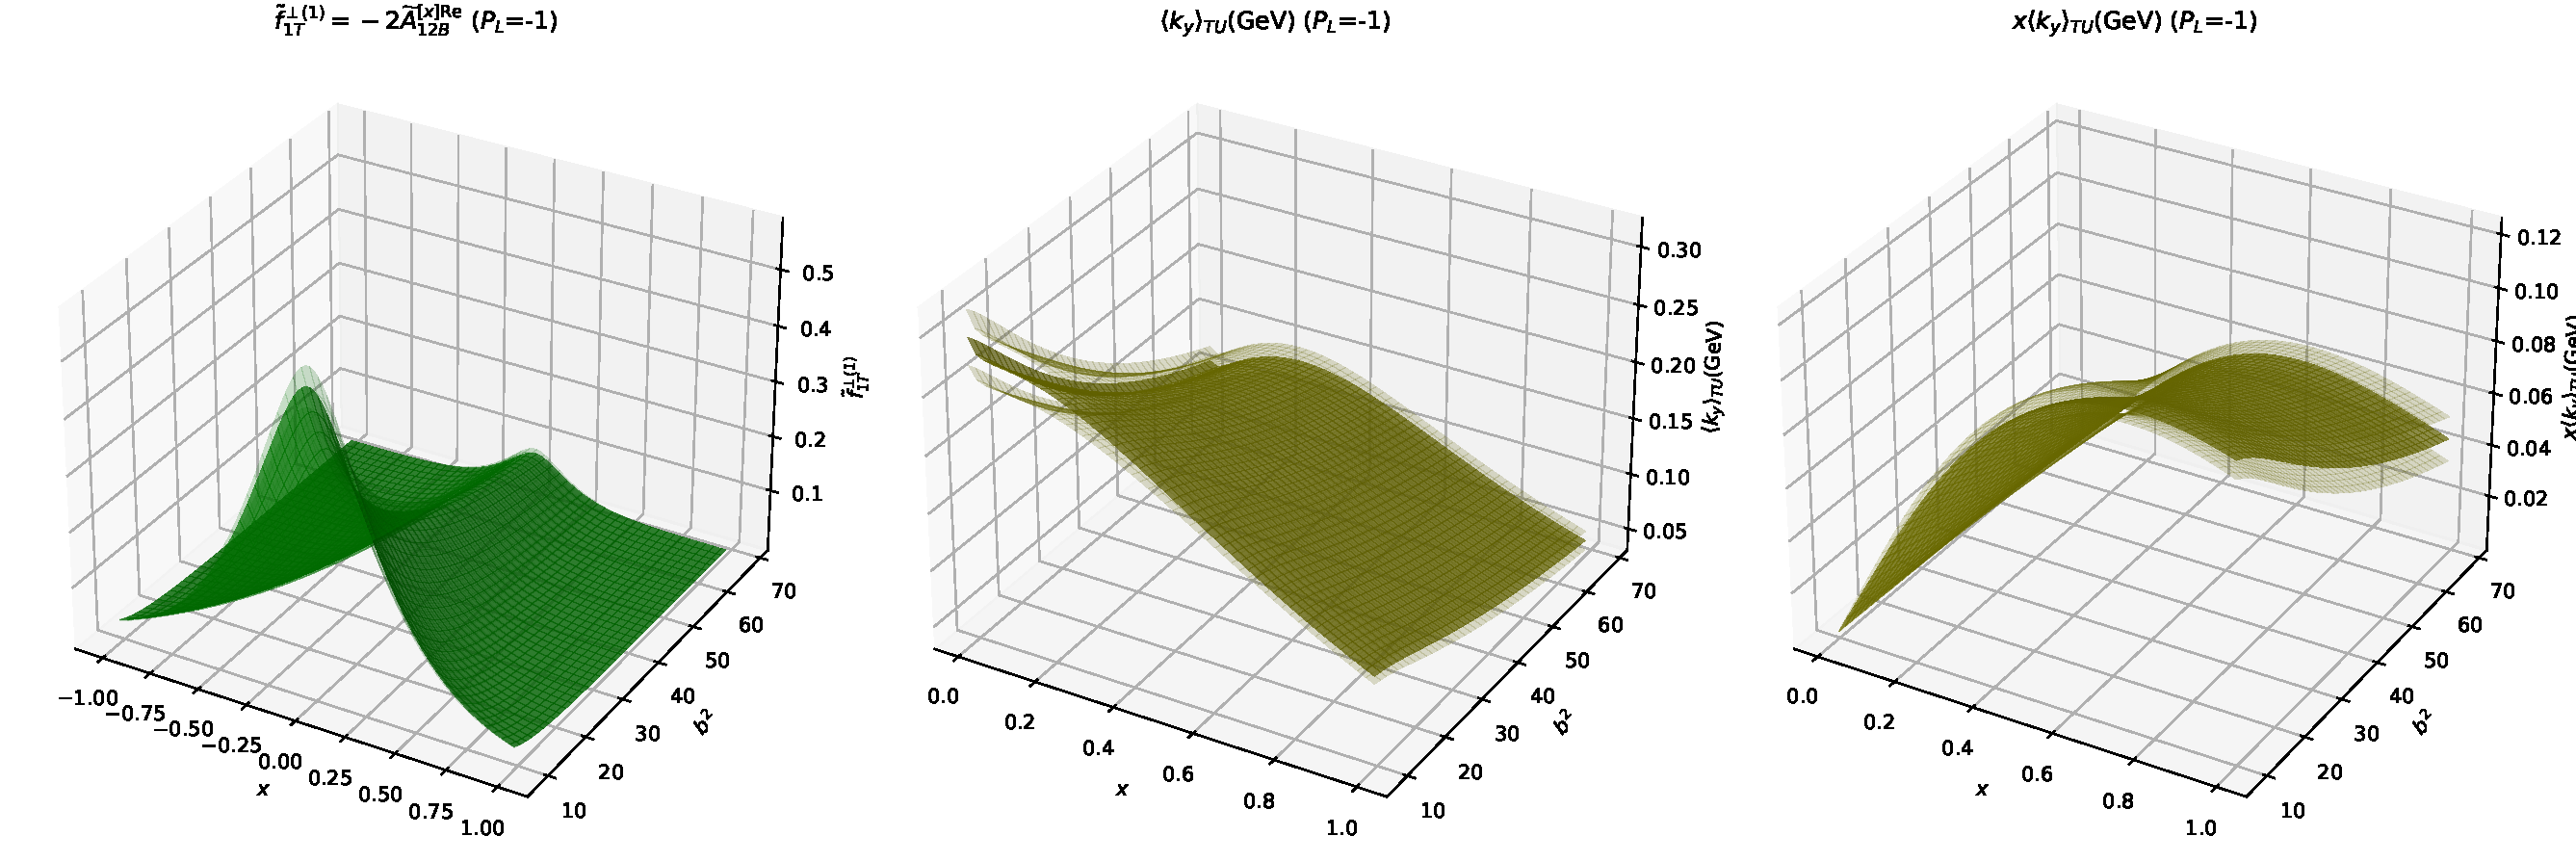
\includegraphics[width=\linewidth,height=.70\textheight,keepaspectratio]{fitting/FT_xdep_3D_A2B_A12B_bmin3_eta610_PL-1__row2.pdf}
\par\small Sivers transform, shift, and $x\langle k_y\rangle_{TU}$. Full $b^2/a^2\in[9,68]$ dependence.

\figsrc{Thesis: SimultaneousFitsCov; FT\_xdep\_3D\_A2B\_A12B\_bmin3\_eta610\_PL-1}
\end{frame}

\begin{frame}{Simultaneous fit parameters: $P_L=-2$}
\small $|\vect b|\ge3a$, $6\le\eta\le10$; reported $\chi^2_{\rm aug}/N_{\rm data}=1.197(85)$.\par\medskip
\begin{columns}[t]\begin{column}{.32\textwidth}\centering $\tAmp_{2B}^{\mathrm{Re}}$\par\medskip\renewcommand{\arraystretch}{1.3}\begin{tabular}{cc}\toprule Parameter & Value\\\midrule
$a$ & $3.9833(80)$ \\
$c$ & $0.166(35)$ \\
$d$ & $0.1020(46)$ \\
$k_1$ & $12.305(14)$ \\
$k_2$ & $-36.1919(27)$ \\
$j$ & $2.061(20)$ \\
$f$ & $0.5357(66)$ \\\bottomrule\end{tabular}\end{column}\begin{column}{.32\textwidth}\centering $\tAmp_{2B}^{\mathrm{Im}}$\par\medskip\renewcommand{\arraystretch}{1.3}\begin{tabular}{cc}\toprule Parameter & Value\\\midrule
$a''$ & $0.368(12)$ \\
$c''$ & $0.1346(69)$ \\
$d''$ & $0.1305(67)$ \\
$j''$ & $1.141(20)$ \\
$f$ & $0.5357(66)$ \\\bottomrule\end{tabular}\end{column}\begin{column}{.32\textwidth}\centering $\tAmp_{12B}^{\mathrm{Re}}$\par\medskip\renewcommand{\arraystretch}{1.3}\begin{tabular}{cc}\toprule Parameter & Value\\\midrule
$a'$ & $0.632(19)$ \\
$c'$ & $0.0769(54)$ \\
$d'$ & $0.0741(52)$ \\
$j'$ & $2.0141(69)$ \\
$f$ & $0.5357(66)$ \\\bottomrule\end{tabular}\end{column}\end{columns}
\figsrc{Thesis: SimultaneousFitsCov/Fit\_Table\_PL-2\_bmin3.tex}
\end{frame}

\begin{frame}{Global fit: $\tAmp_{2B}^{\mathrm{Re}}$, $P_L=-2$}
\centering
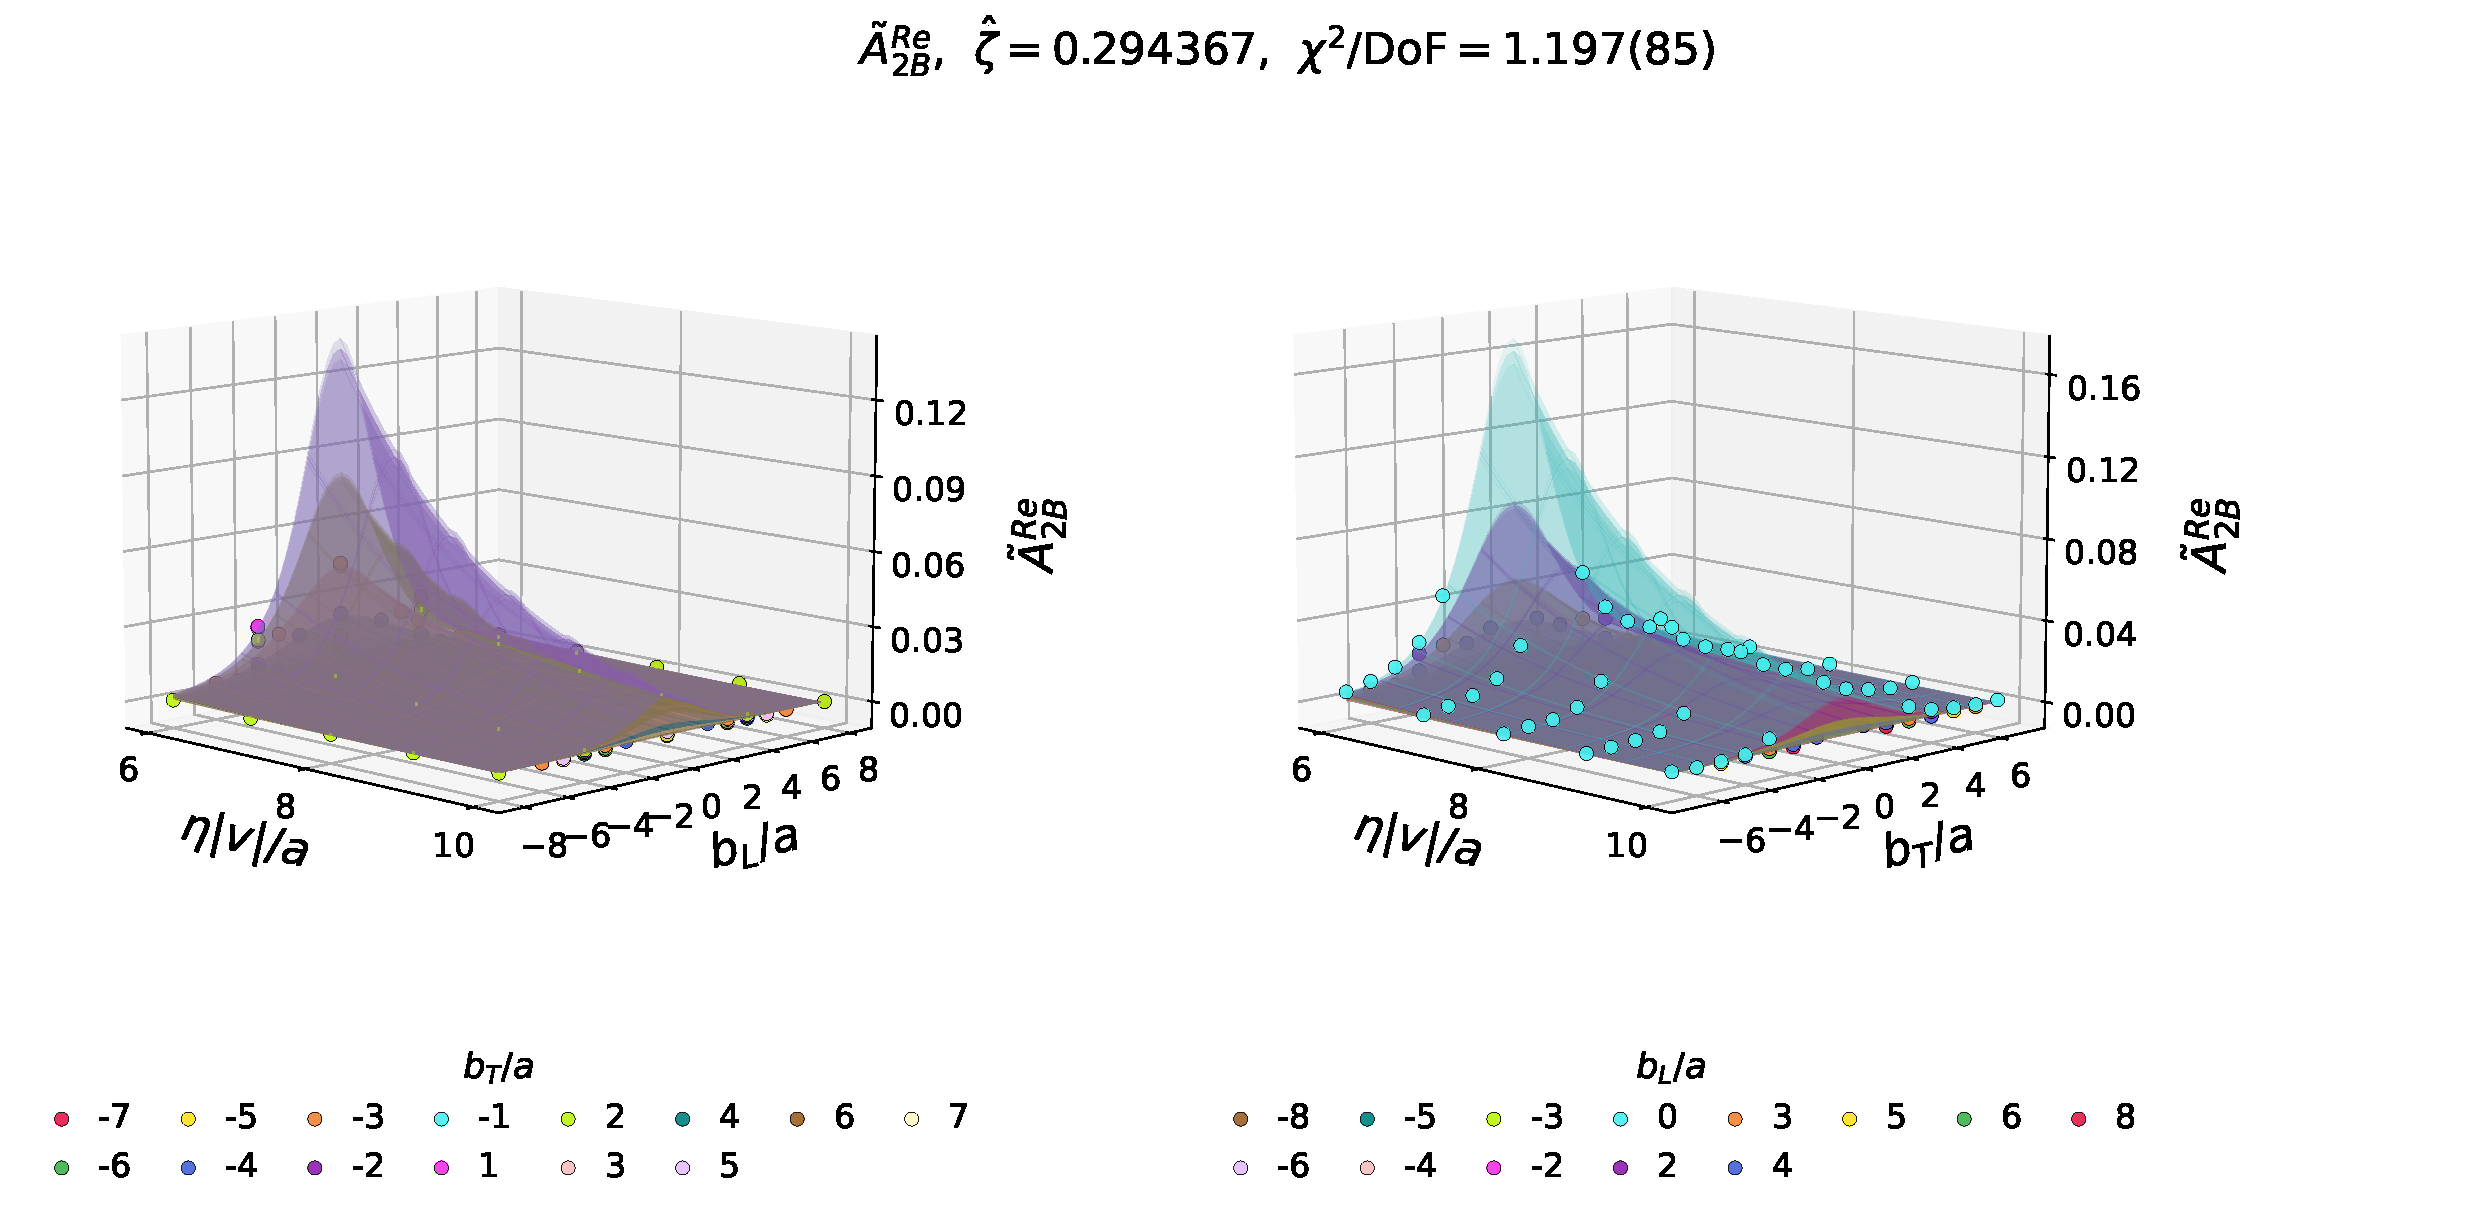
\includegraphics[width=\linewidth,height=.70\textheight,keepaspectratio]{fitting/ReA2B_PL-2_WithFit_3D.pdf}
\par\small Spatial coordinates: $(b_L,b_T,\eta)$. All panels and data overlays retained.

\figsrc{Thesis: plots; ReA2B\_PL-2\_WithFit\_3D}
\end{frame}

\begin{frame}{Global fit: $\tAmp_{2B}^{\mathrm{Re}}$, $P_L=-2$}
\centering
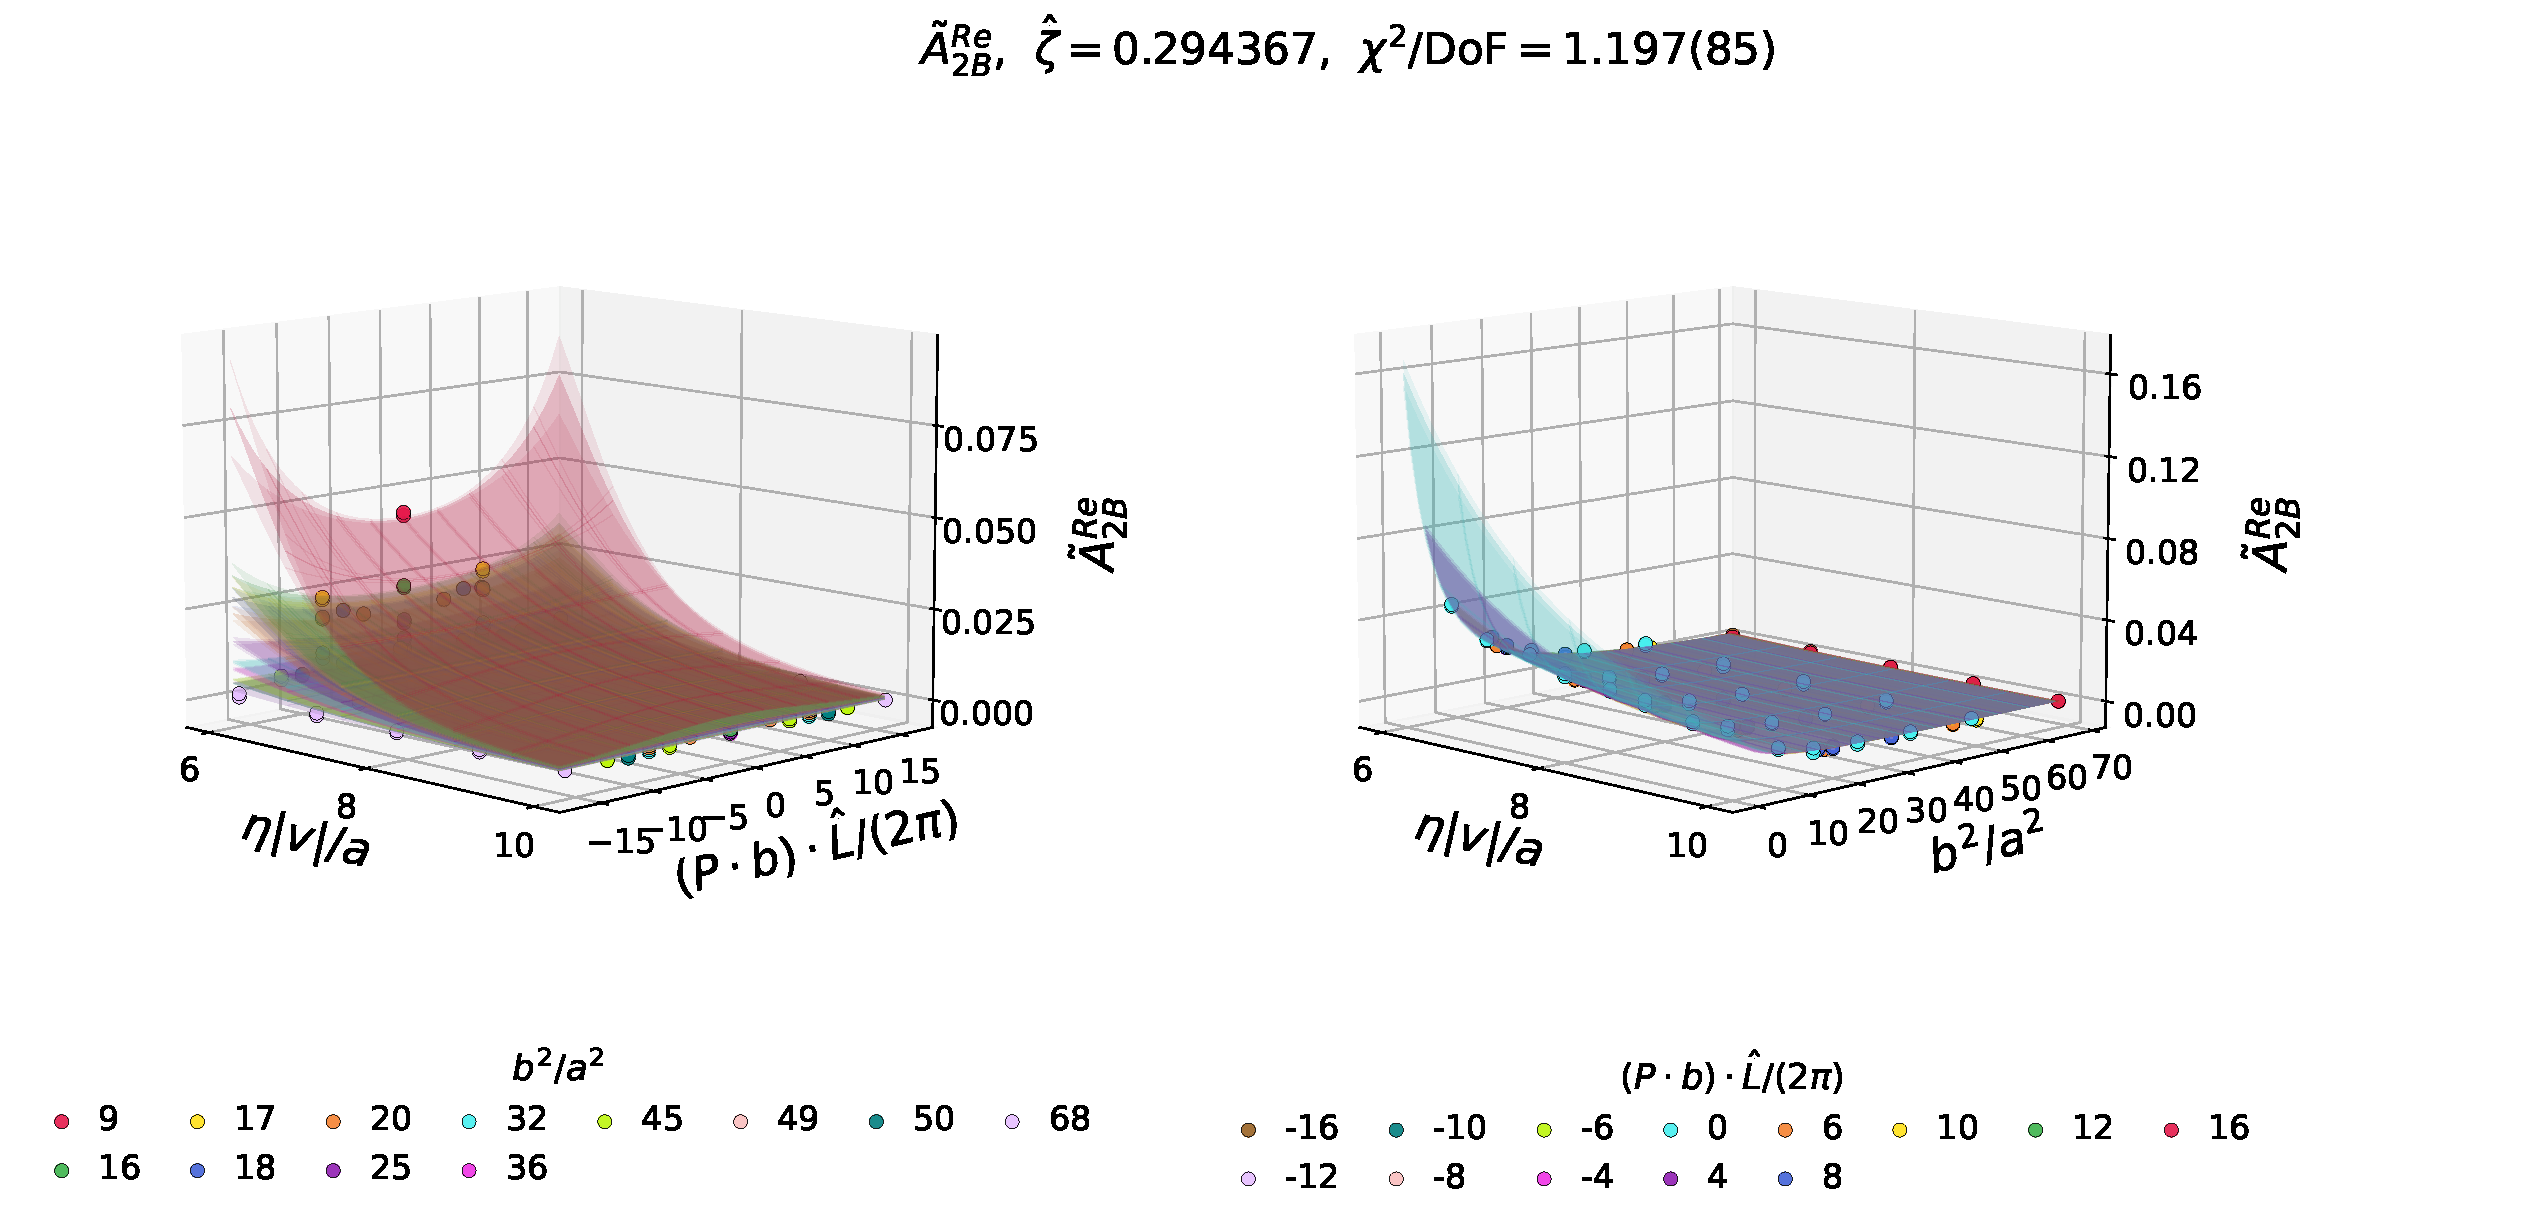
\includegraphics[width=\linewidth,height=.70\textheight,keepaspectratio]{fitting/ReA2B_Pb_bsq_PL-2_WithFit_3D.pdf}
\par\small Invariant coordinates: $(\nu,b^2,\eta)$. All panels and data overlays retained.

\figsrc{Thesis: plots; ReA2B\_Pb\_bsq\_PL-2\_WithFit\_3D}
\end{frame}

\begin{frame}{Fixed staple $\eta=8$: $\tAmp_{2B}^{\mathrm{Re}}$, $P_L=-2$}
\centering
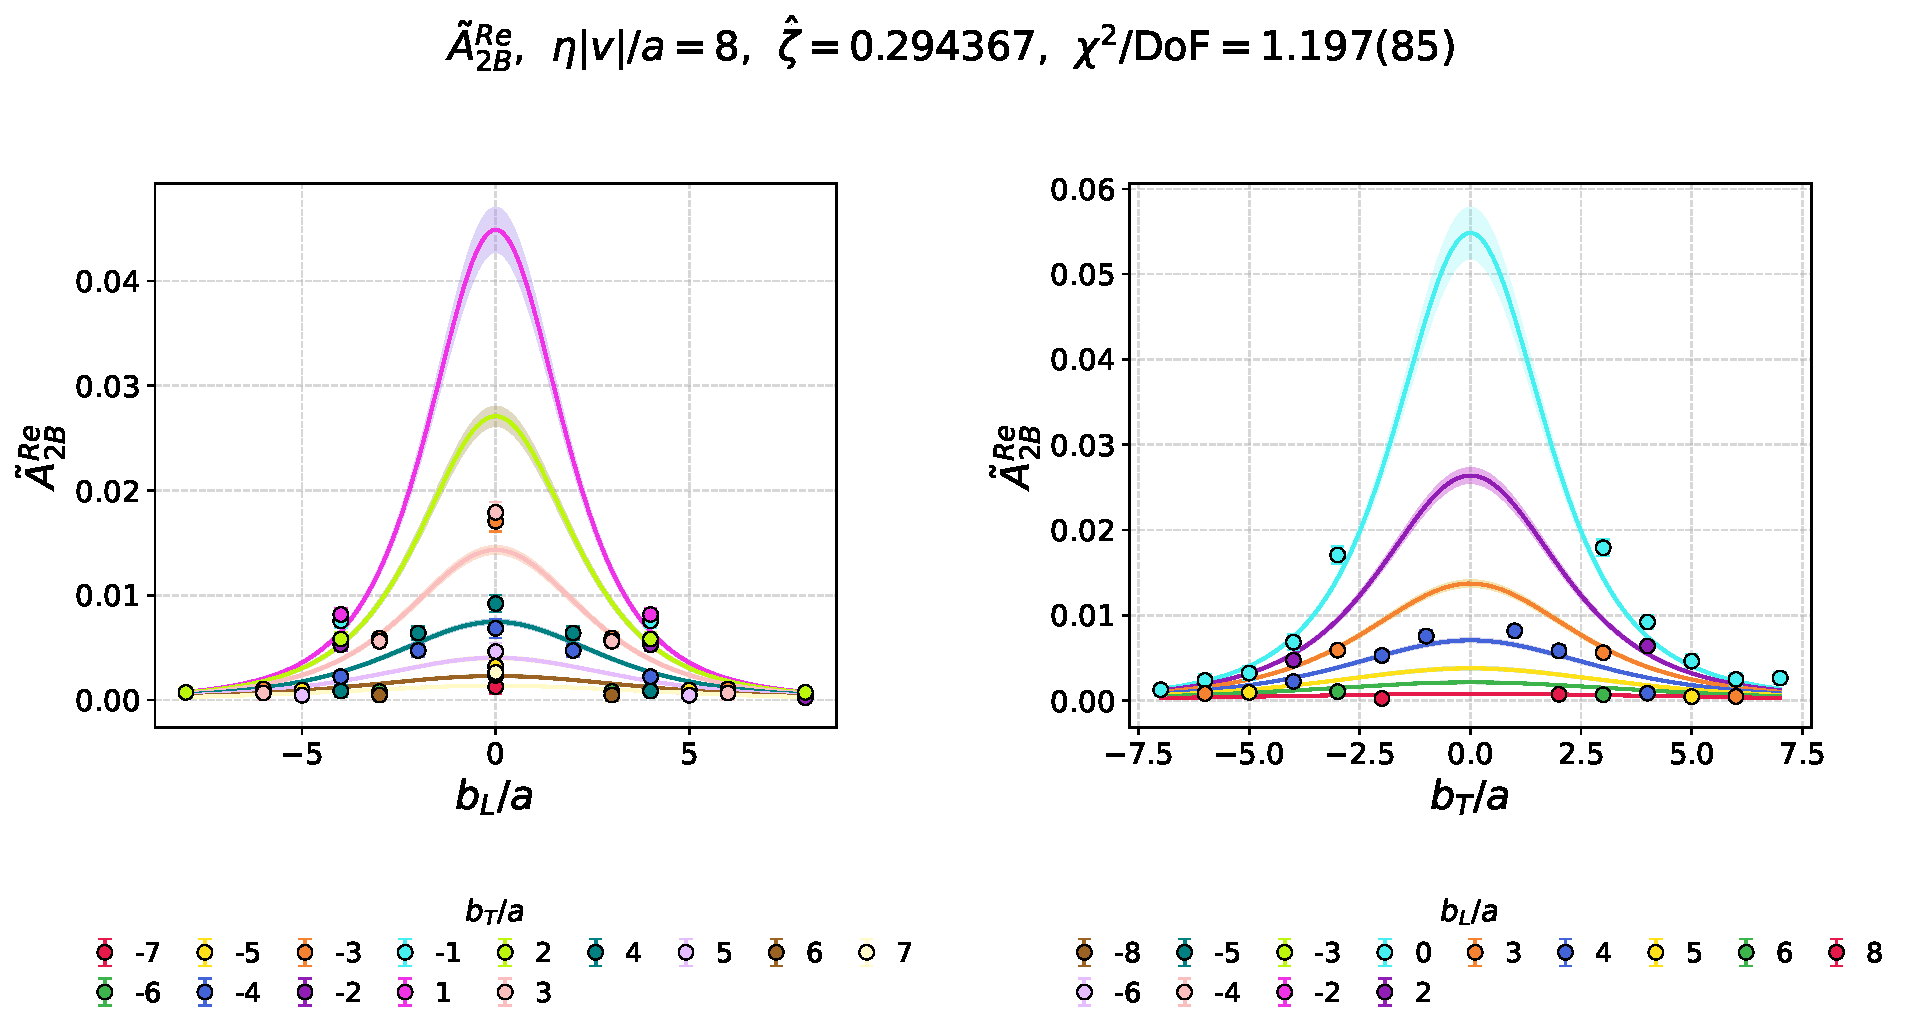
\includegraphics[width=\linewidth,height=.70\textheight,keepaspectratio]{fitting/ReA2B_eta8_PL-2_WithFit_2D.pdf}
\par\small Both spatial-coordinate slices. Same simultaneous fit, with Jackknife bands.

\figsrc{Thesis: plots; ReA2B\_eta8\_PL-2\_WithFit\_2D}
\end{frame}

\begin{frame}{Fixed staple $\eta=8$: $\tAmp_{2B}^{\mathrm{Re}}$, $P_L=-2$}
\centering
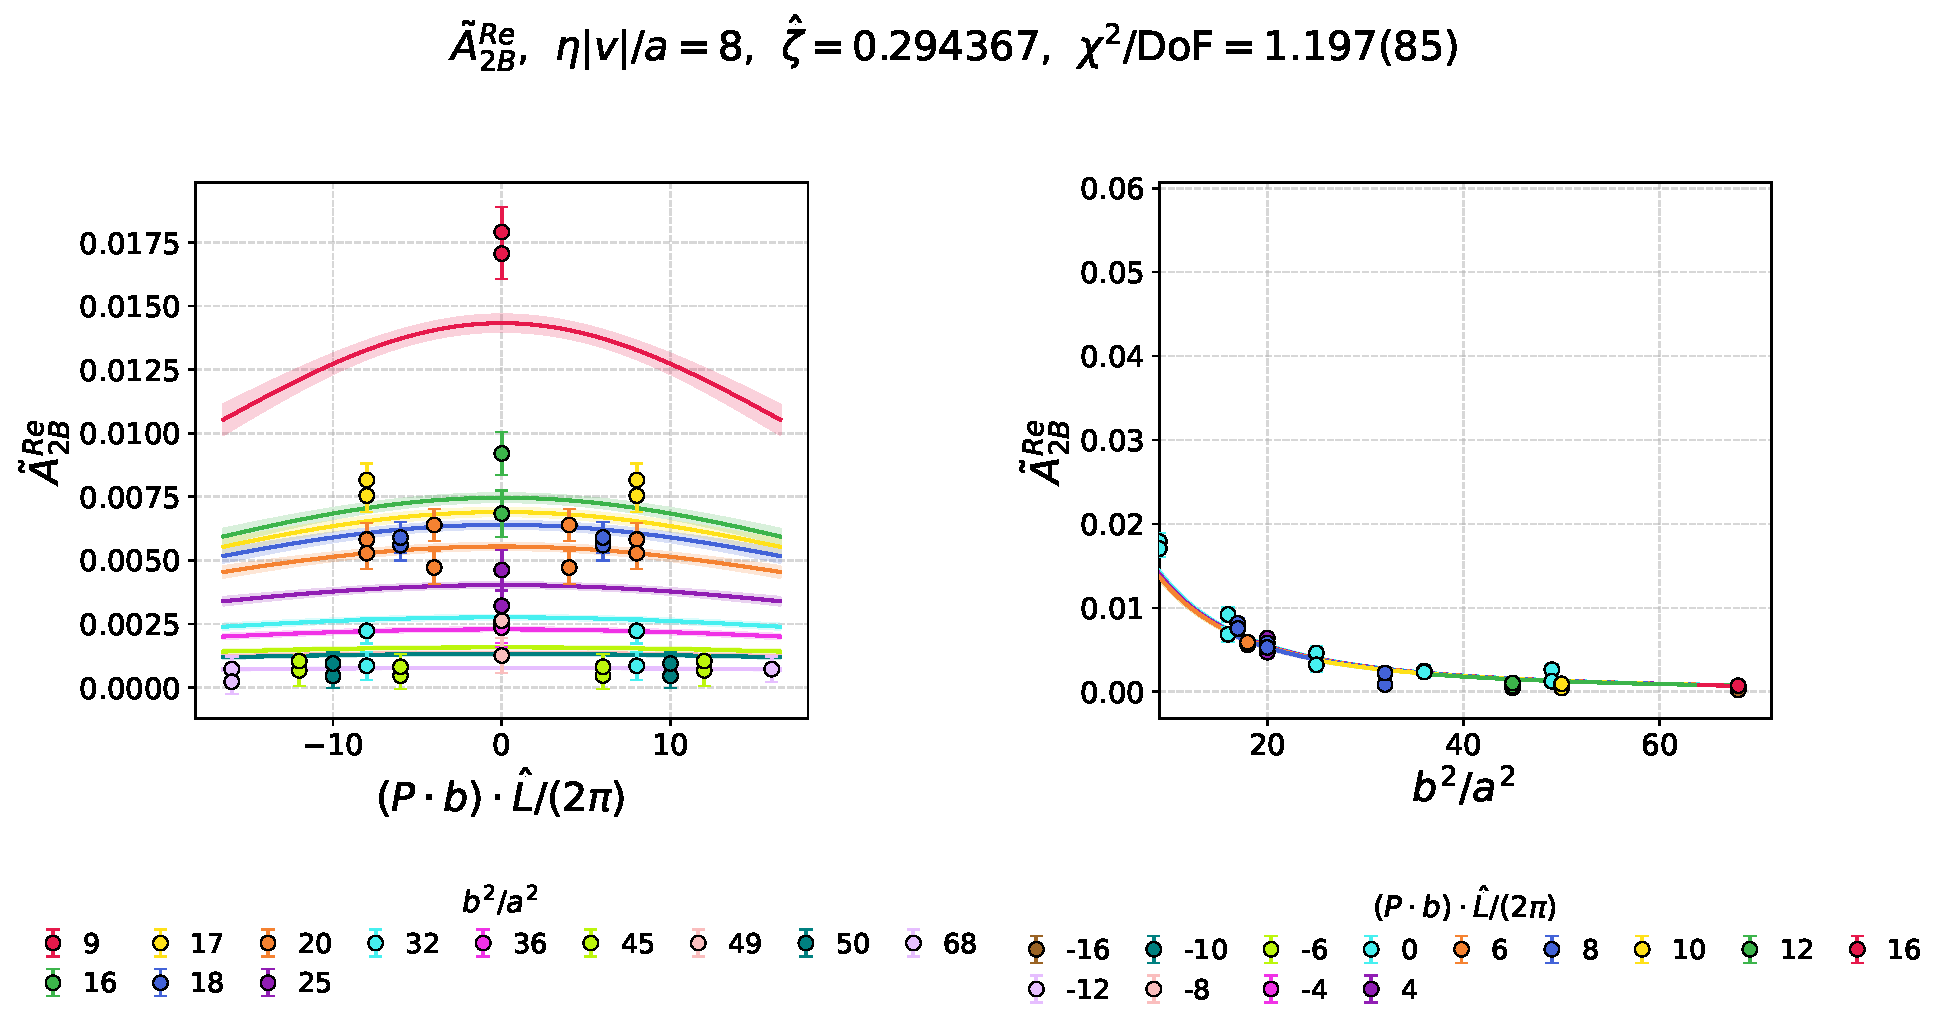
\includegraphics[width=\linewidth,height=.70\textheight,keepaspectratio]{fitting/ReA2B_Pb_bsq_eta8_PL-2_WithFit_2D.pdf}
\par\small Both invariant-coordinate slices. Same simultaneous fit, with Jackknife bands.

\figsrc{Thesis: plots; ReA2B\_Pb\_bsq\_eta8\_PL-2\_WithFit\_2D}
\end{frame}

\begin{frame}{Global fit: $\tAmp_{2B}^{\mathrm{Im}}$, $P_L=-2$}
\centering
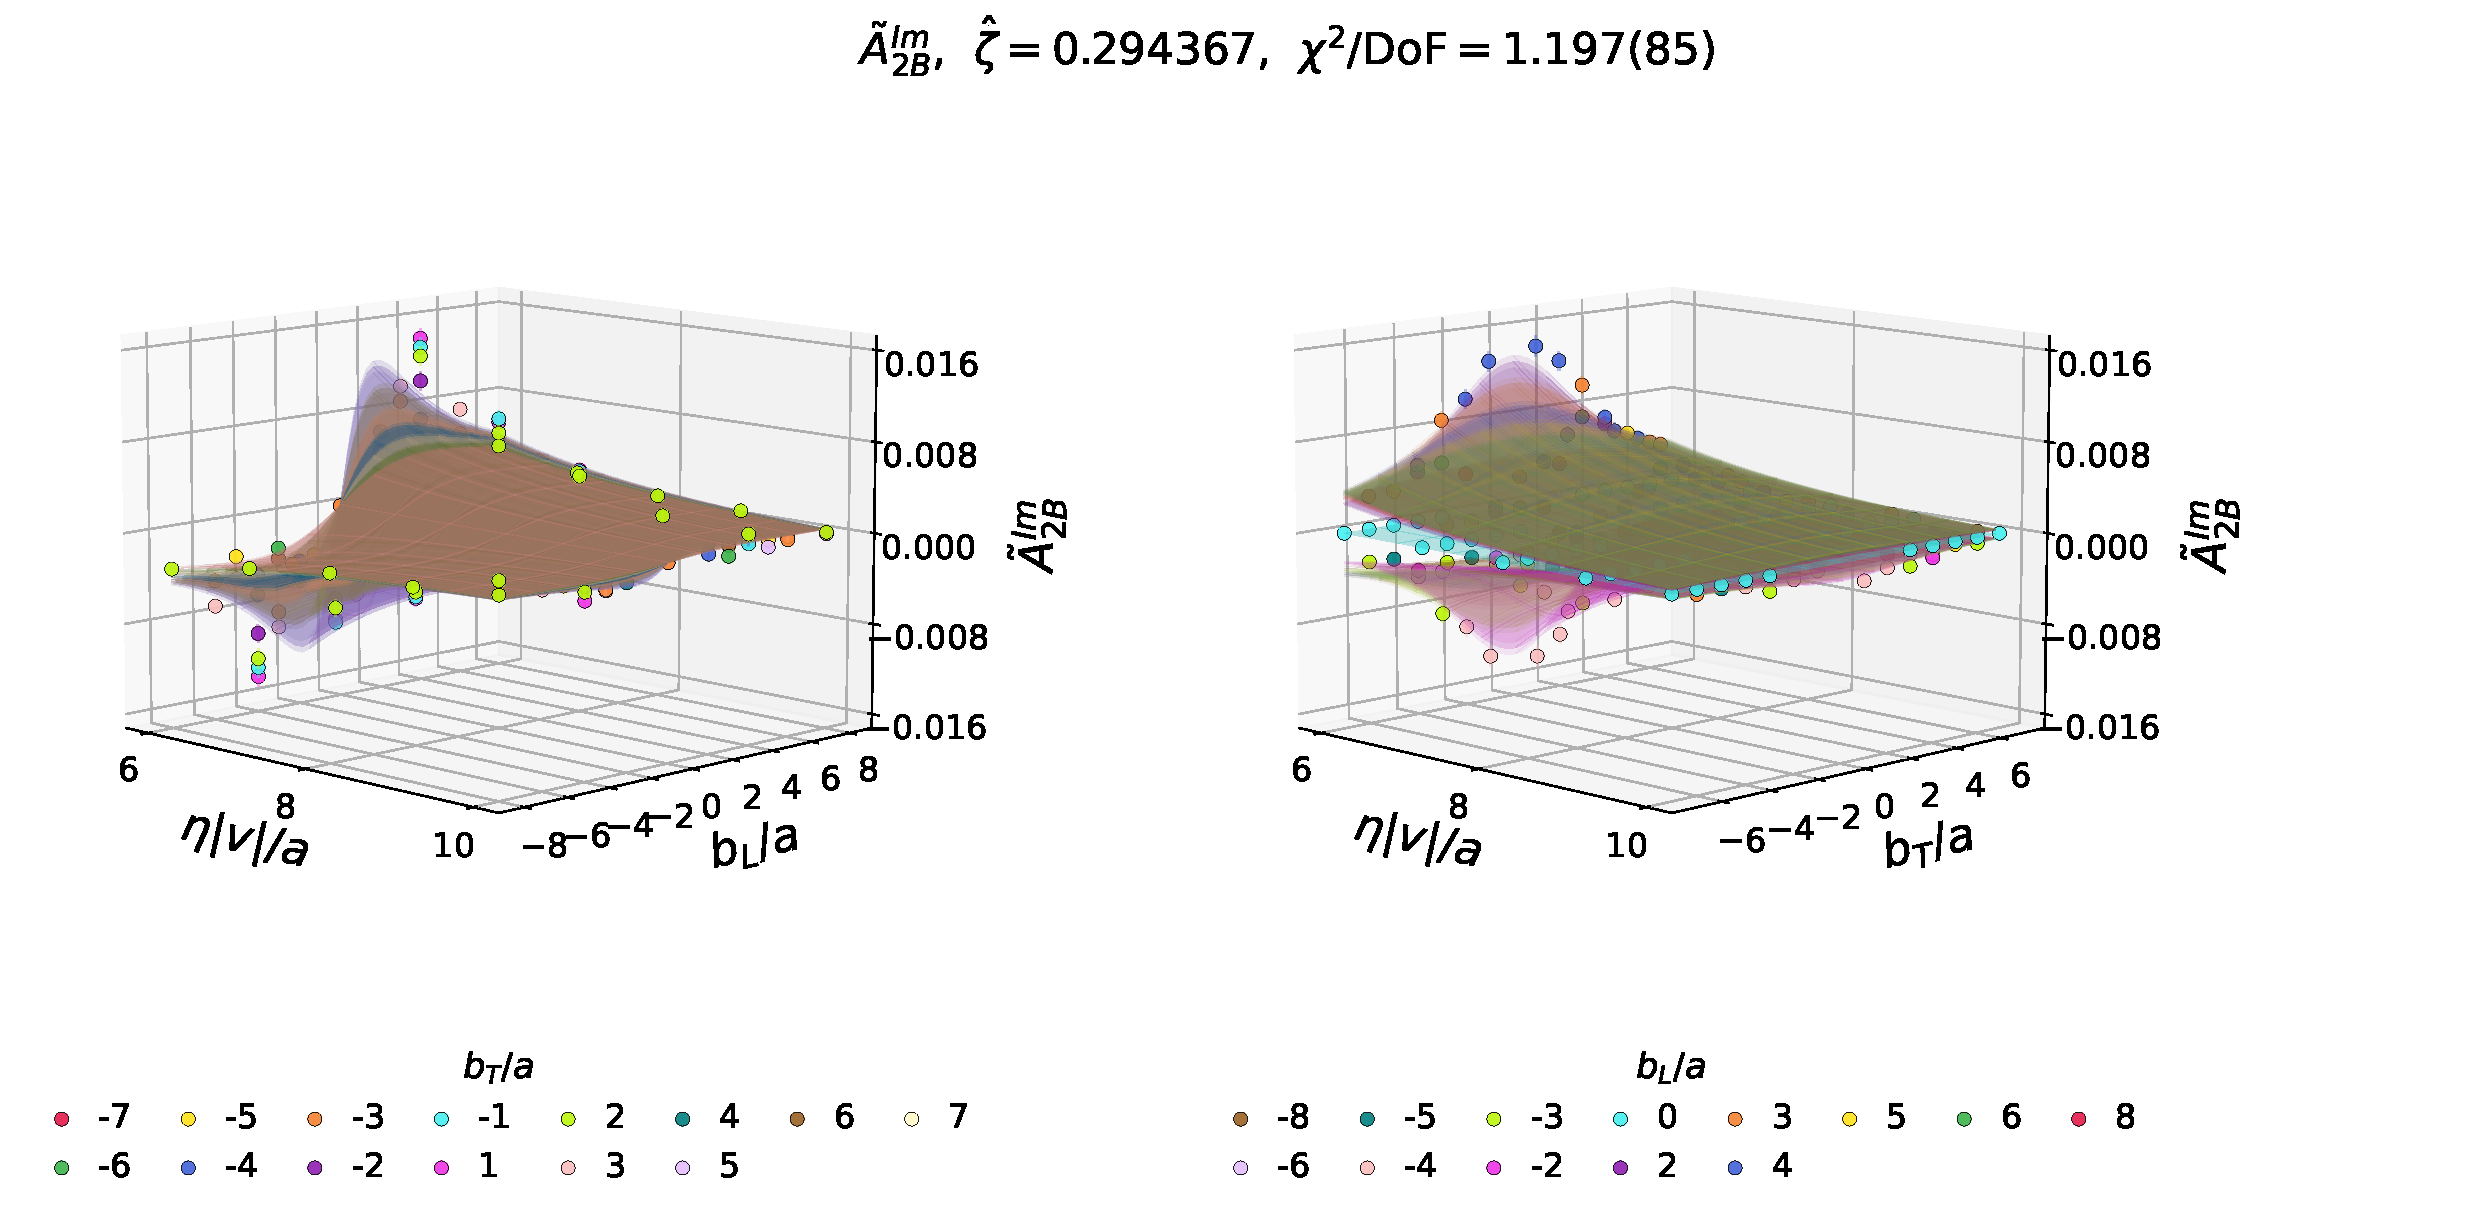
\includegraphics[width=\linewidth,height=.70\textheight,keepaspectratio]{fitting/ImA2B_PL-2_WithFit_3D.pdf}
\par\small Spatial coordinates: $(b_L,b_T,\eta)$. All panels and data overlays retained.

\figsrc{Thesis: plots; ImA2B\_PL-2\_WithFit\_3D}
\end{frame}

\begin{frame}{Global fit: $\tAmp_{2B}^{\mathrm{Im}}$, $P_L=-2$}
\centering
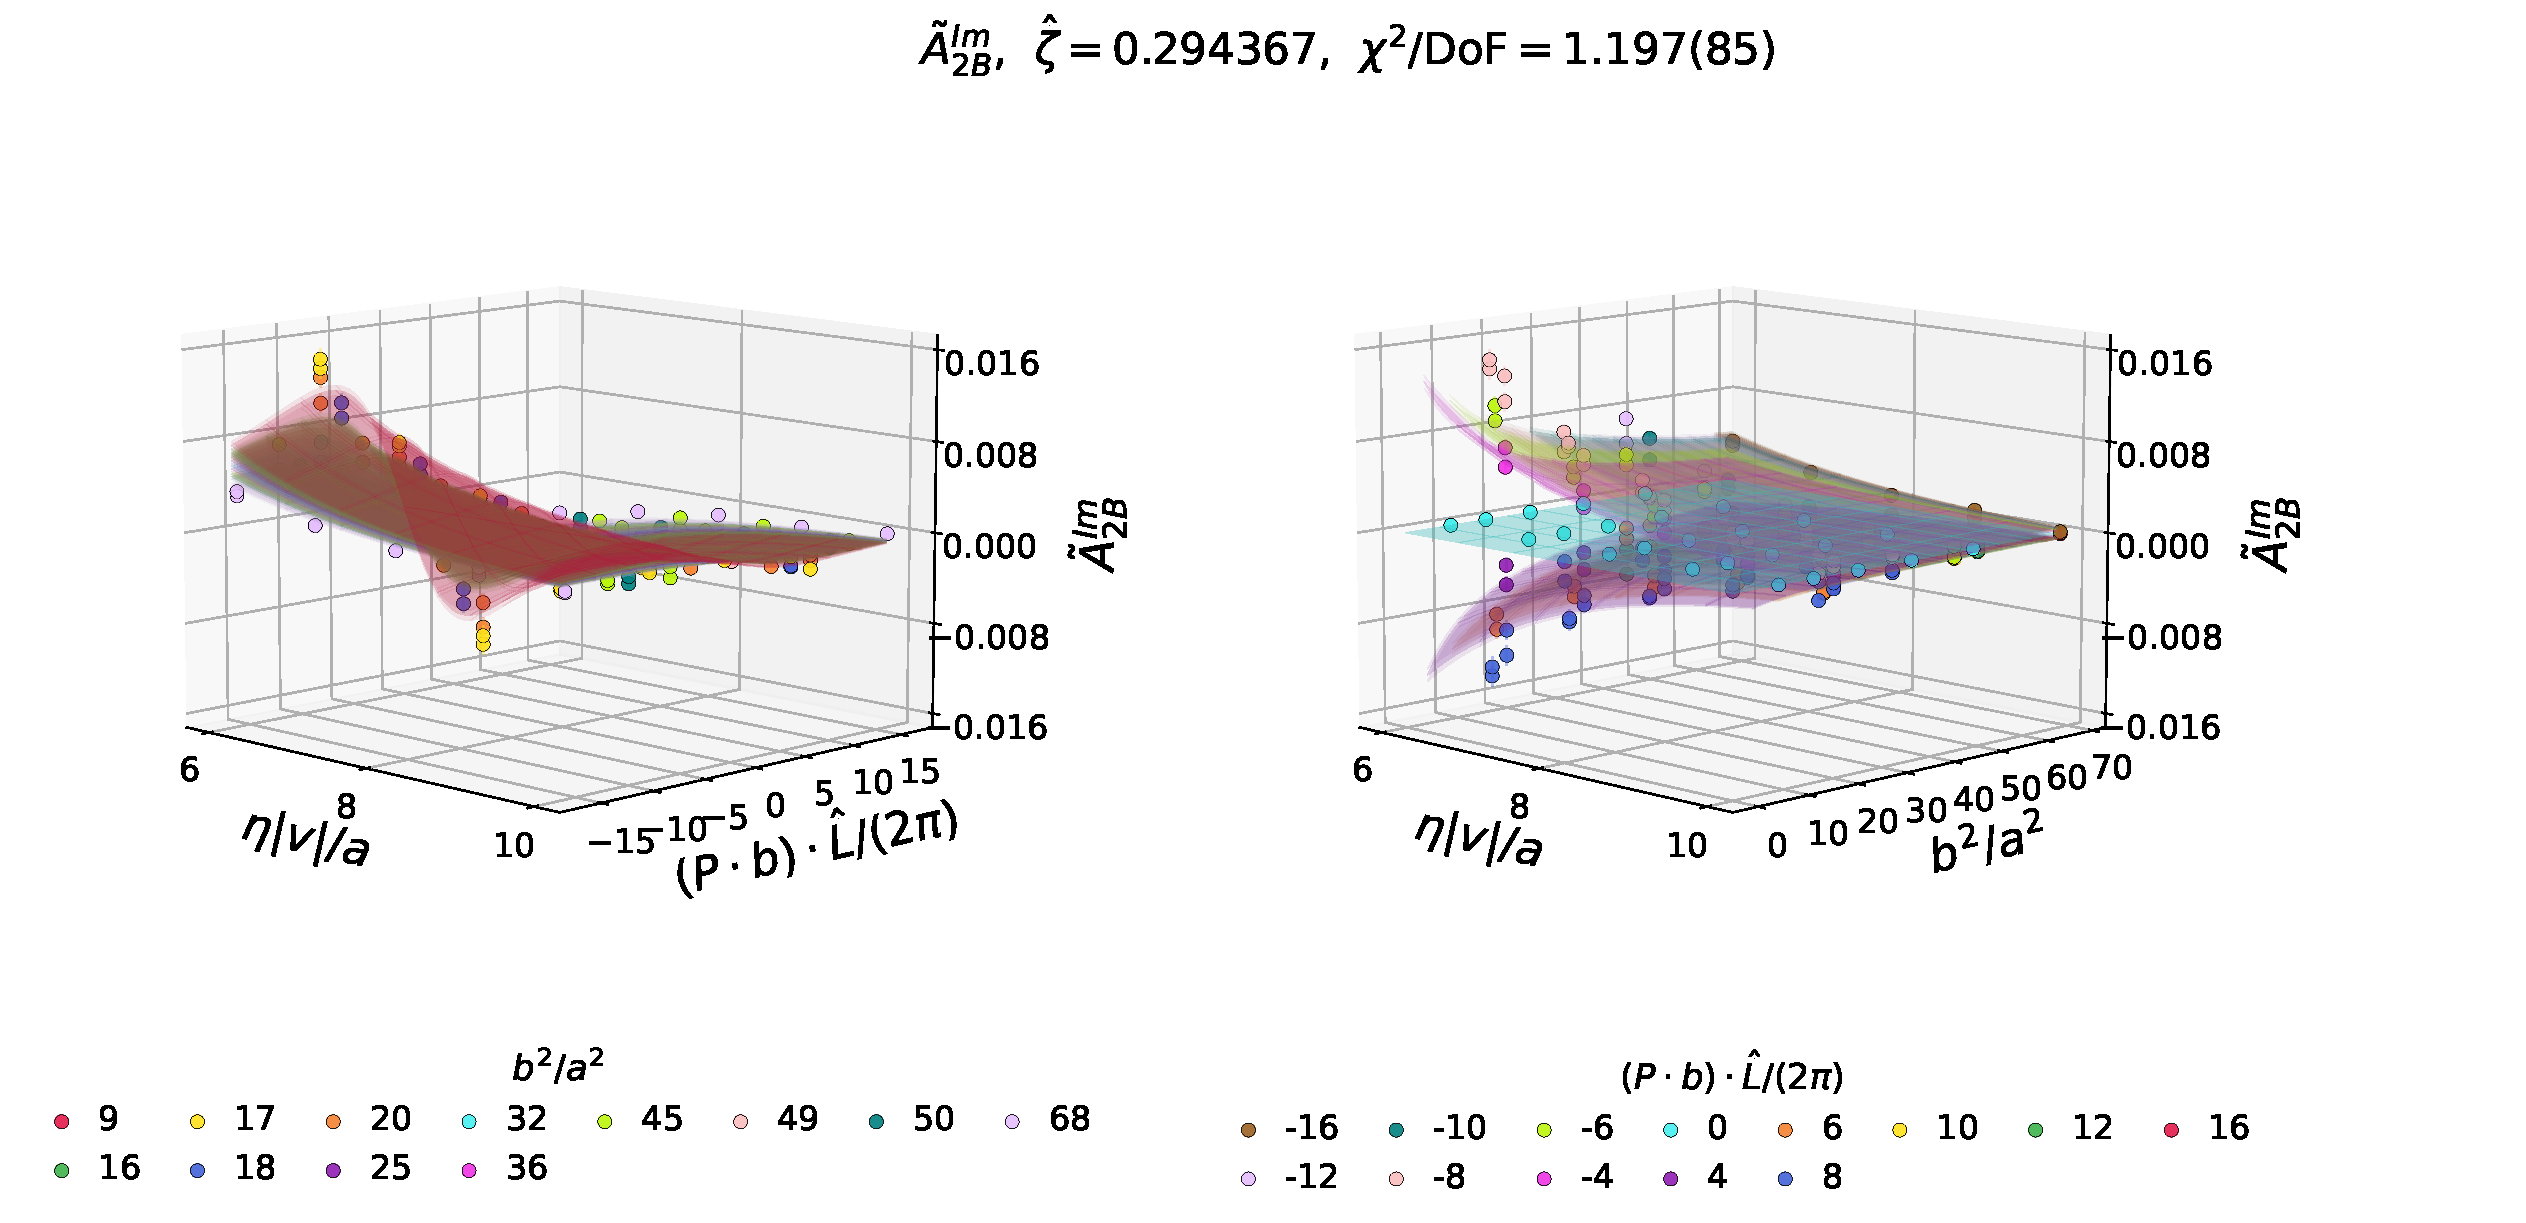
\includegraphics[width=\linewidth,height=.70\textheight,keepaspectratio]{fitting/ImA2B_Pb_bsq_PL-2_WithFit_3D.pdf}
\par\small Invariant coordinates: $(\nu,b^2,\eta)$. All panels and data overlays retained.

\figsrc{Thesis: plots; ImA2B\_Pb\_bsq\_PL-2\_WithFit\_3D}
\end{frame}

\begin{frame}{Fixed staple $\eta=8$: $\tAmp_{2B}^{\mathrm{Im}}$, $P_L=-2$}
\centering
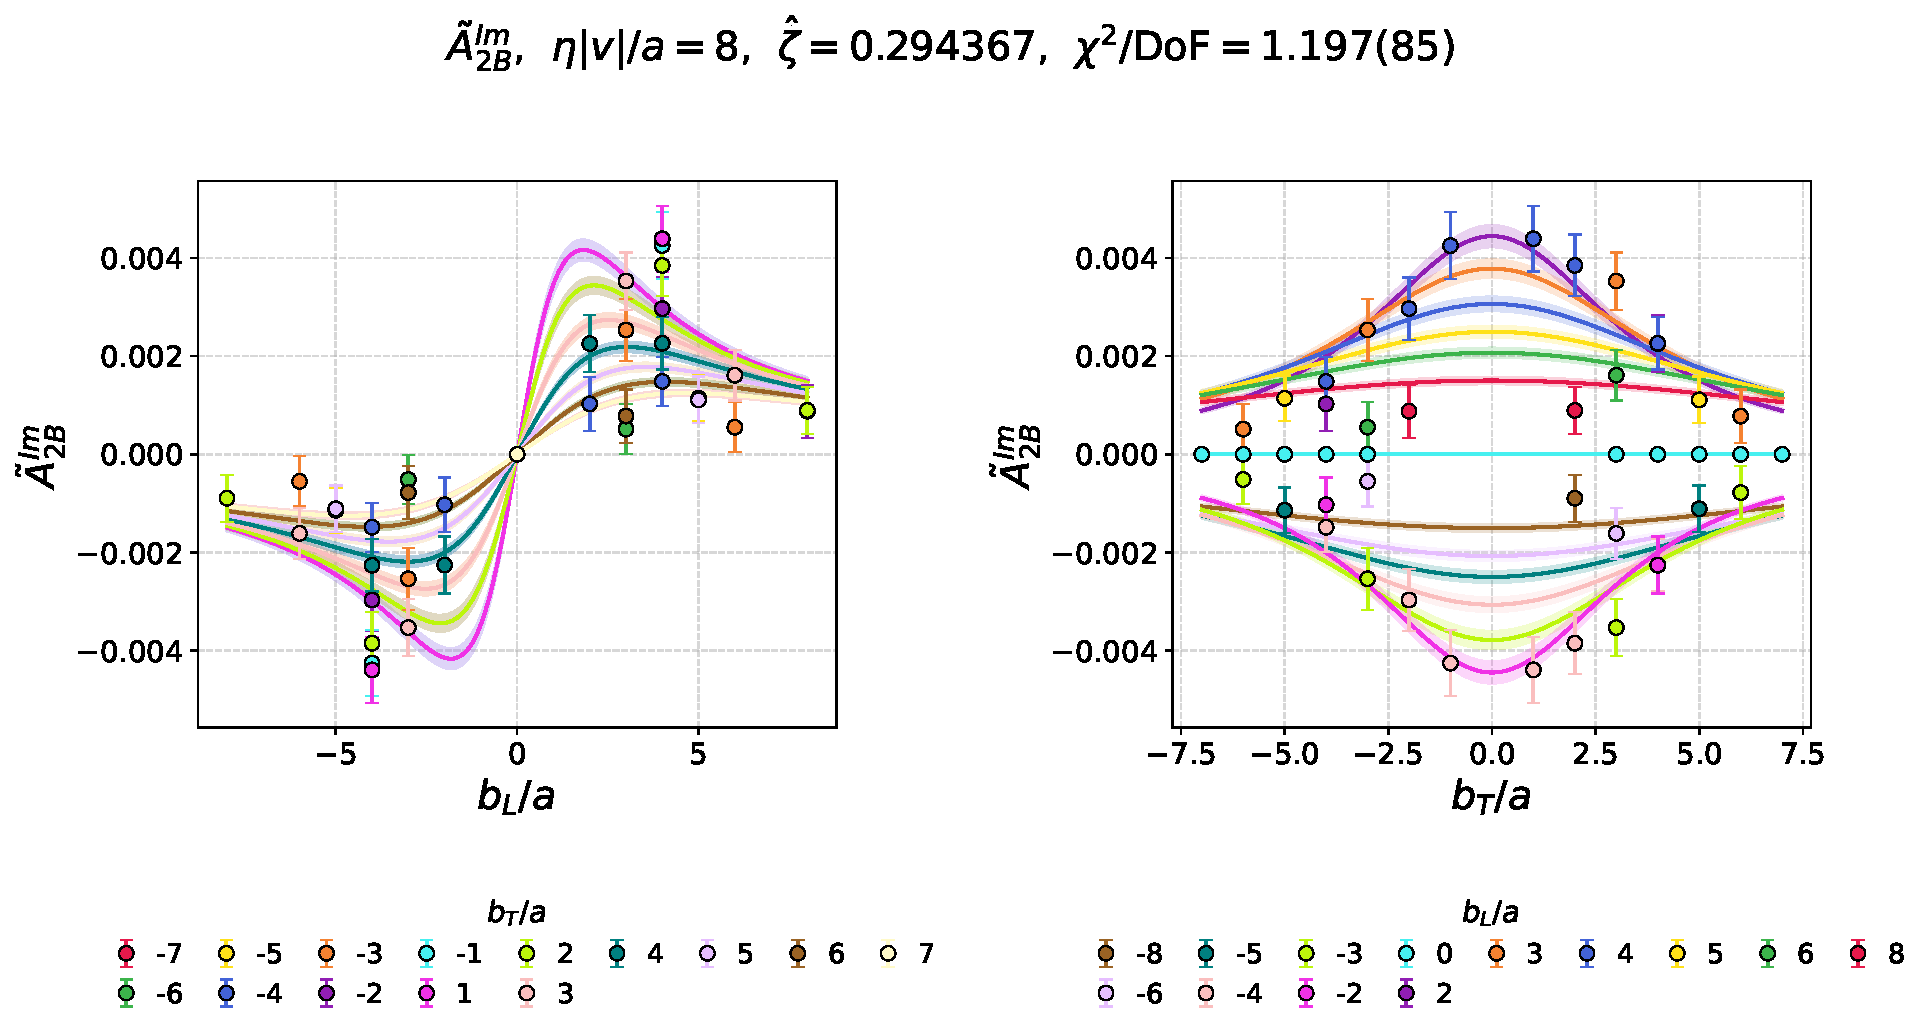
\includegraphics[width=\linewidth,height=.70\textheight,keepaspectratio]{fitting/ImA2B_eta8_PL-2_WithFit_2D.pdf}
\par\small Both spatial-coordinate slices. Same simultaneous fit, with Jackknife bands.

\figsrc{Thesis: plots; ImA2B\_eta8\_PL-2\_WithFit\_2D}
\end{frame}

\begin{frame}{Fixed staple $\eta=8$: $\tAmp_{2B}^{\mathrm{Im}}$, $P_L=-2$}
\centering
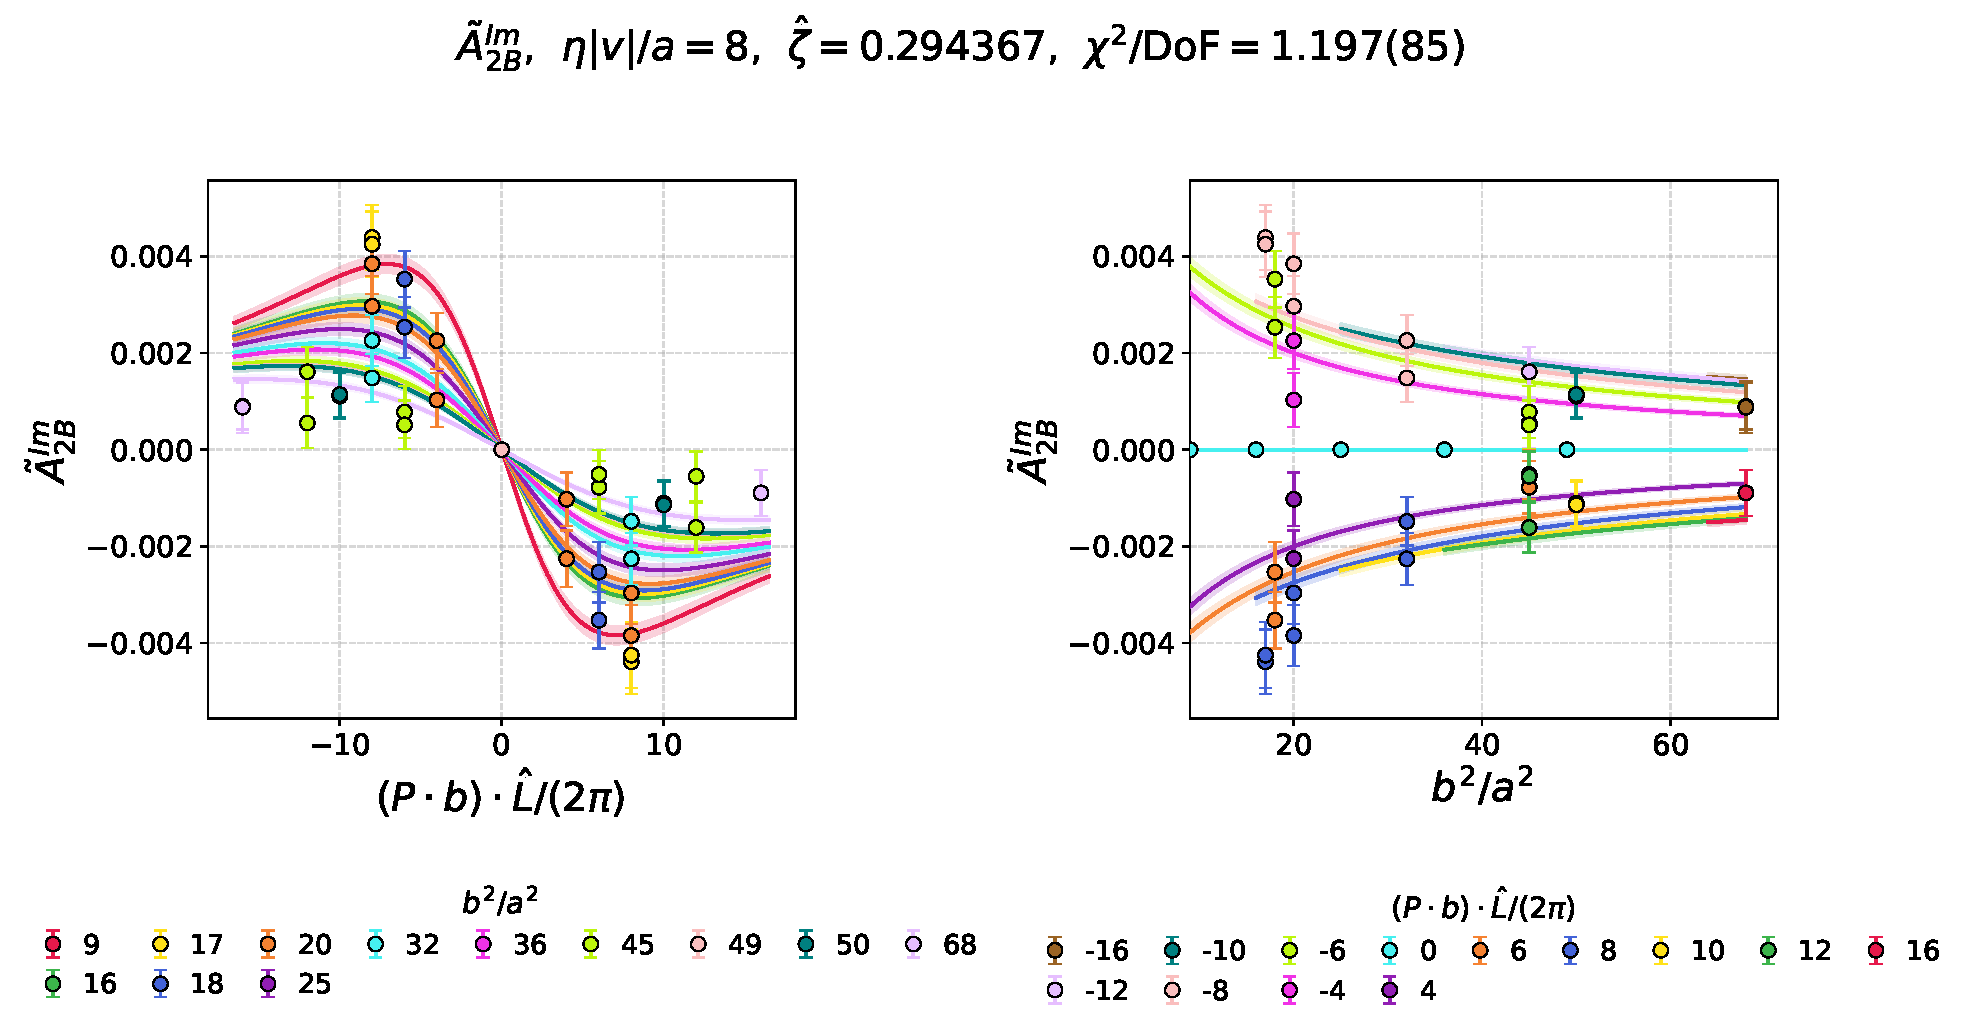
\includegraphics[width=\linewidth,height=.70\textheight,keepaspectratio]{fitting/ImA2B_Pb_bsq_eta8_PL-2_WithFit_2D.pdf}
\par\small Both invariant-coordinate slices. Same simultaneous fit, with Jackknife bands.

\figsrc{Thesis: plots; ImA2B\_Pb\_bsq\_eta8\_PL-2\_WithFit\_2D}
\end{frame}

\begin{frame}{Global fit: $\tAmp_{12B}^{\mathrm{Re}}$, $P_L=-2$}
\centering
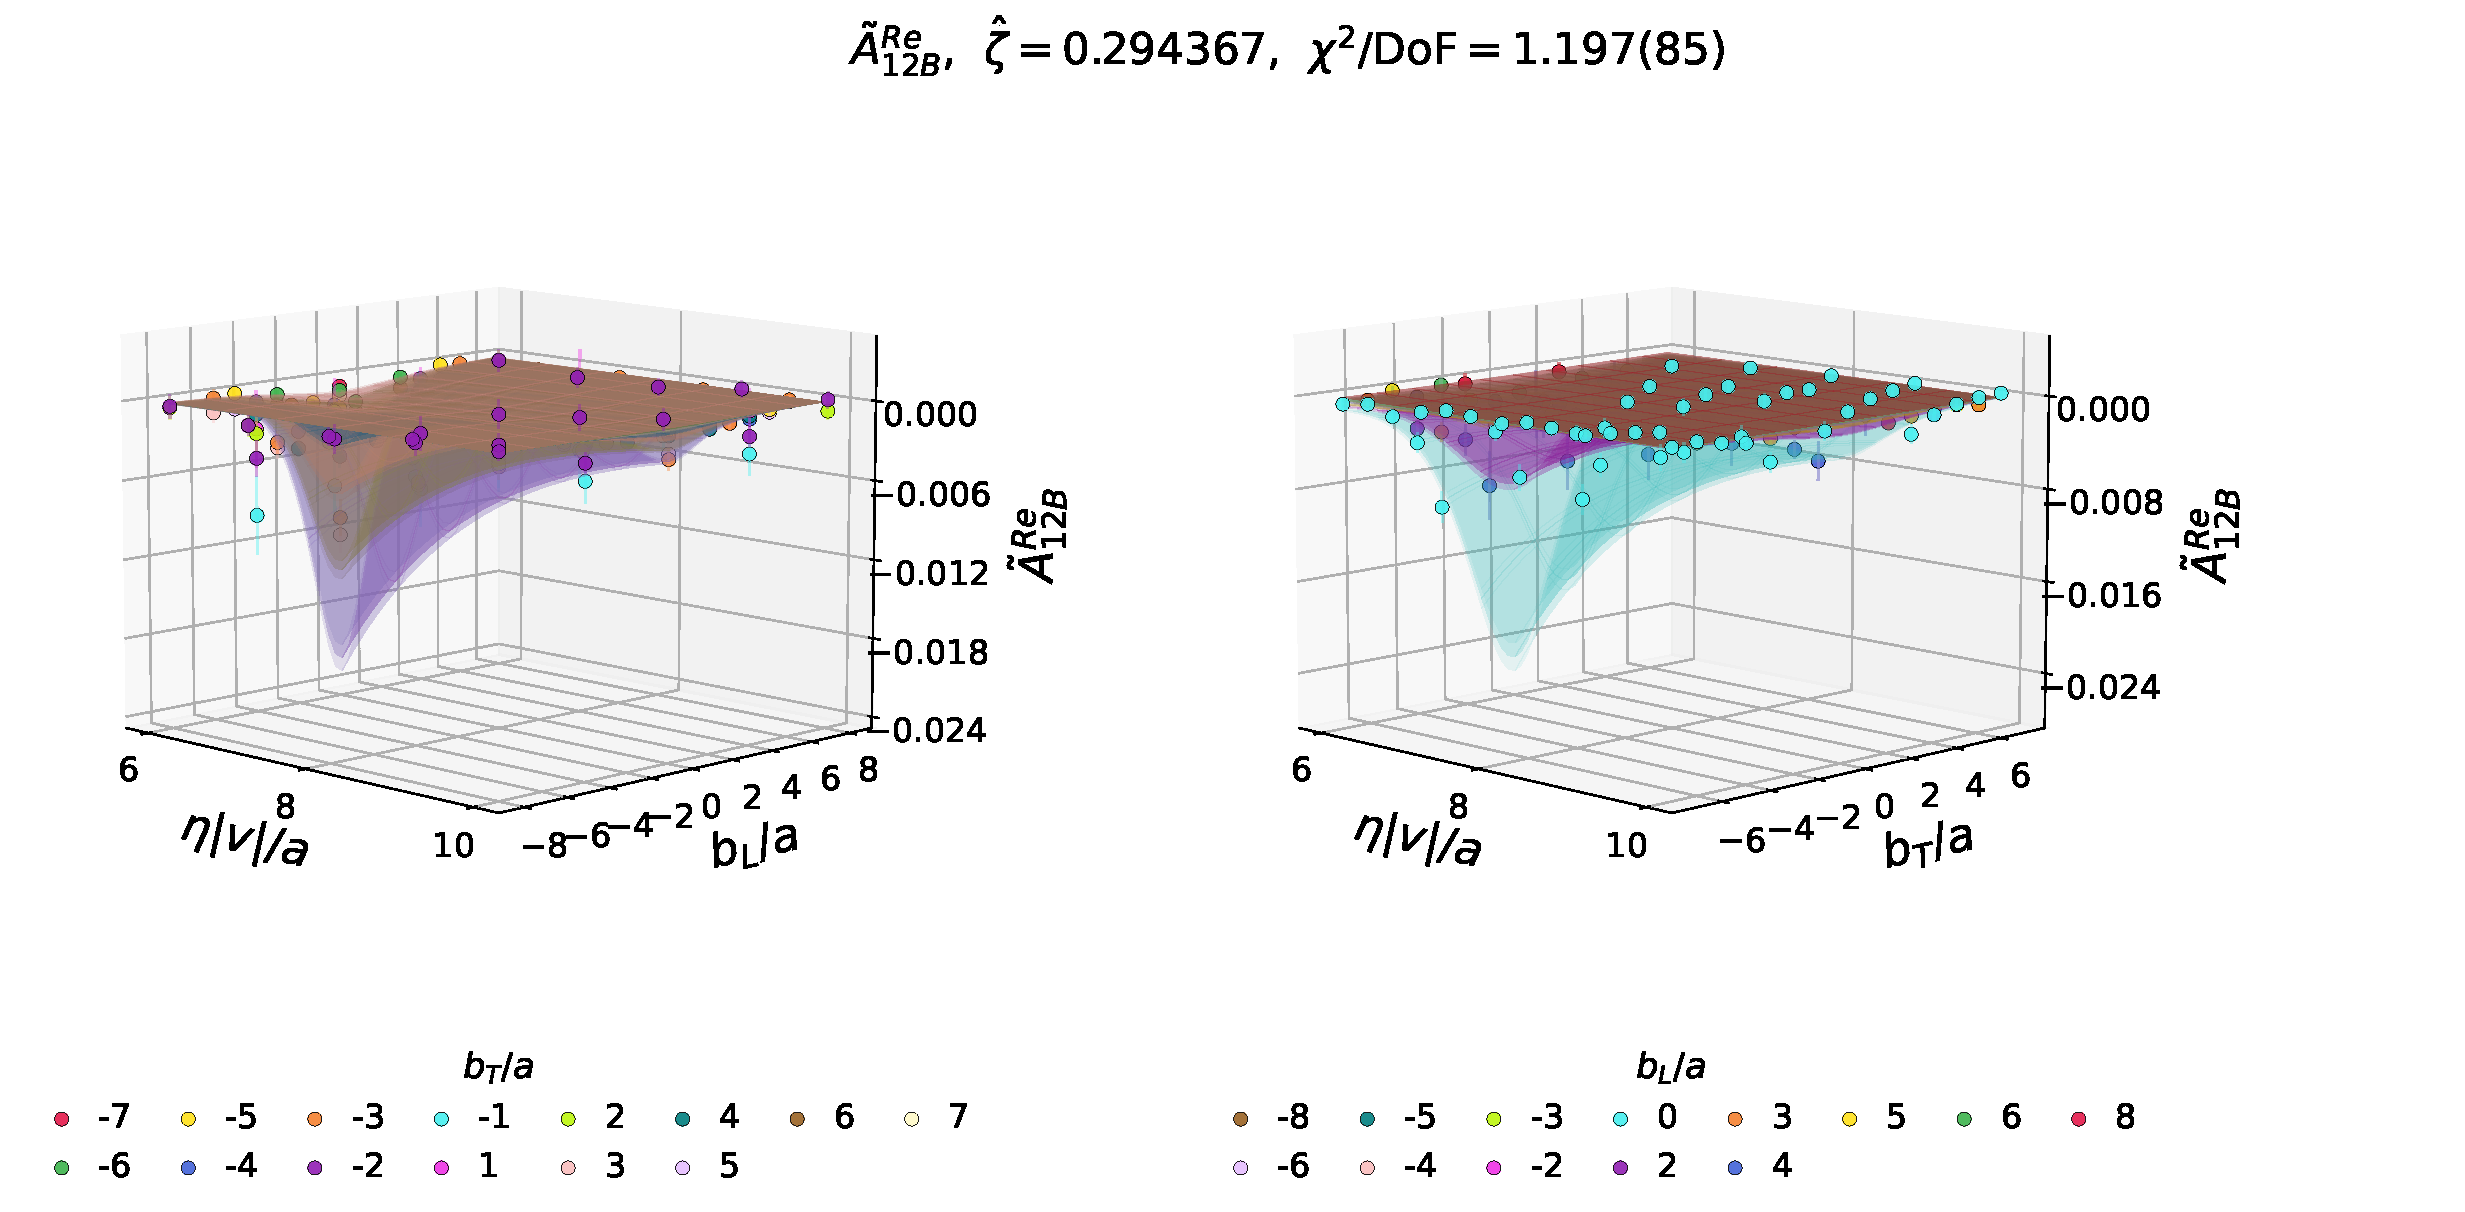
\includegraphics[width=\linewidth,height=.70\textheight,keepaspectratio]{fitting/ReA12B_PL-2_WithFit_3D.pdf}
\par\small Spatial coordinates: $(b_L,b_T,\eta)$. All panels and data overlays retained.

\figsrc{Thesis: plots; ReA12B\_PL-2\_WithFit\_3D}
\end{frame}

\begin{frame}{Global fit: $\tAmp_{12B}^{\mathrm{Re}}$, $P_L=-2$}
\centering
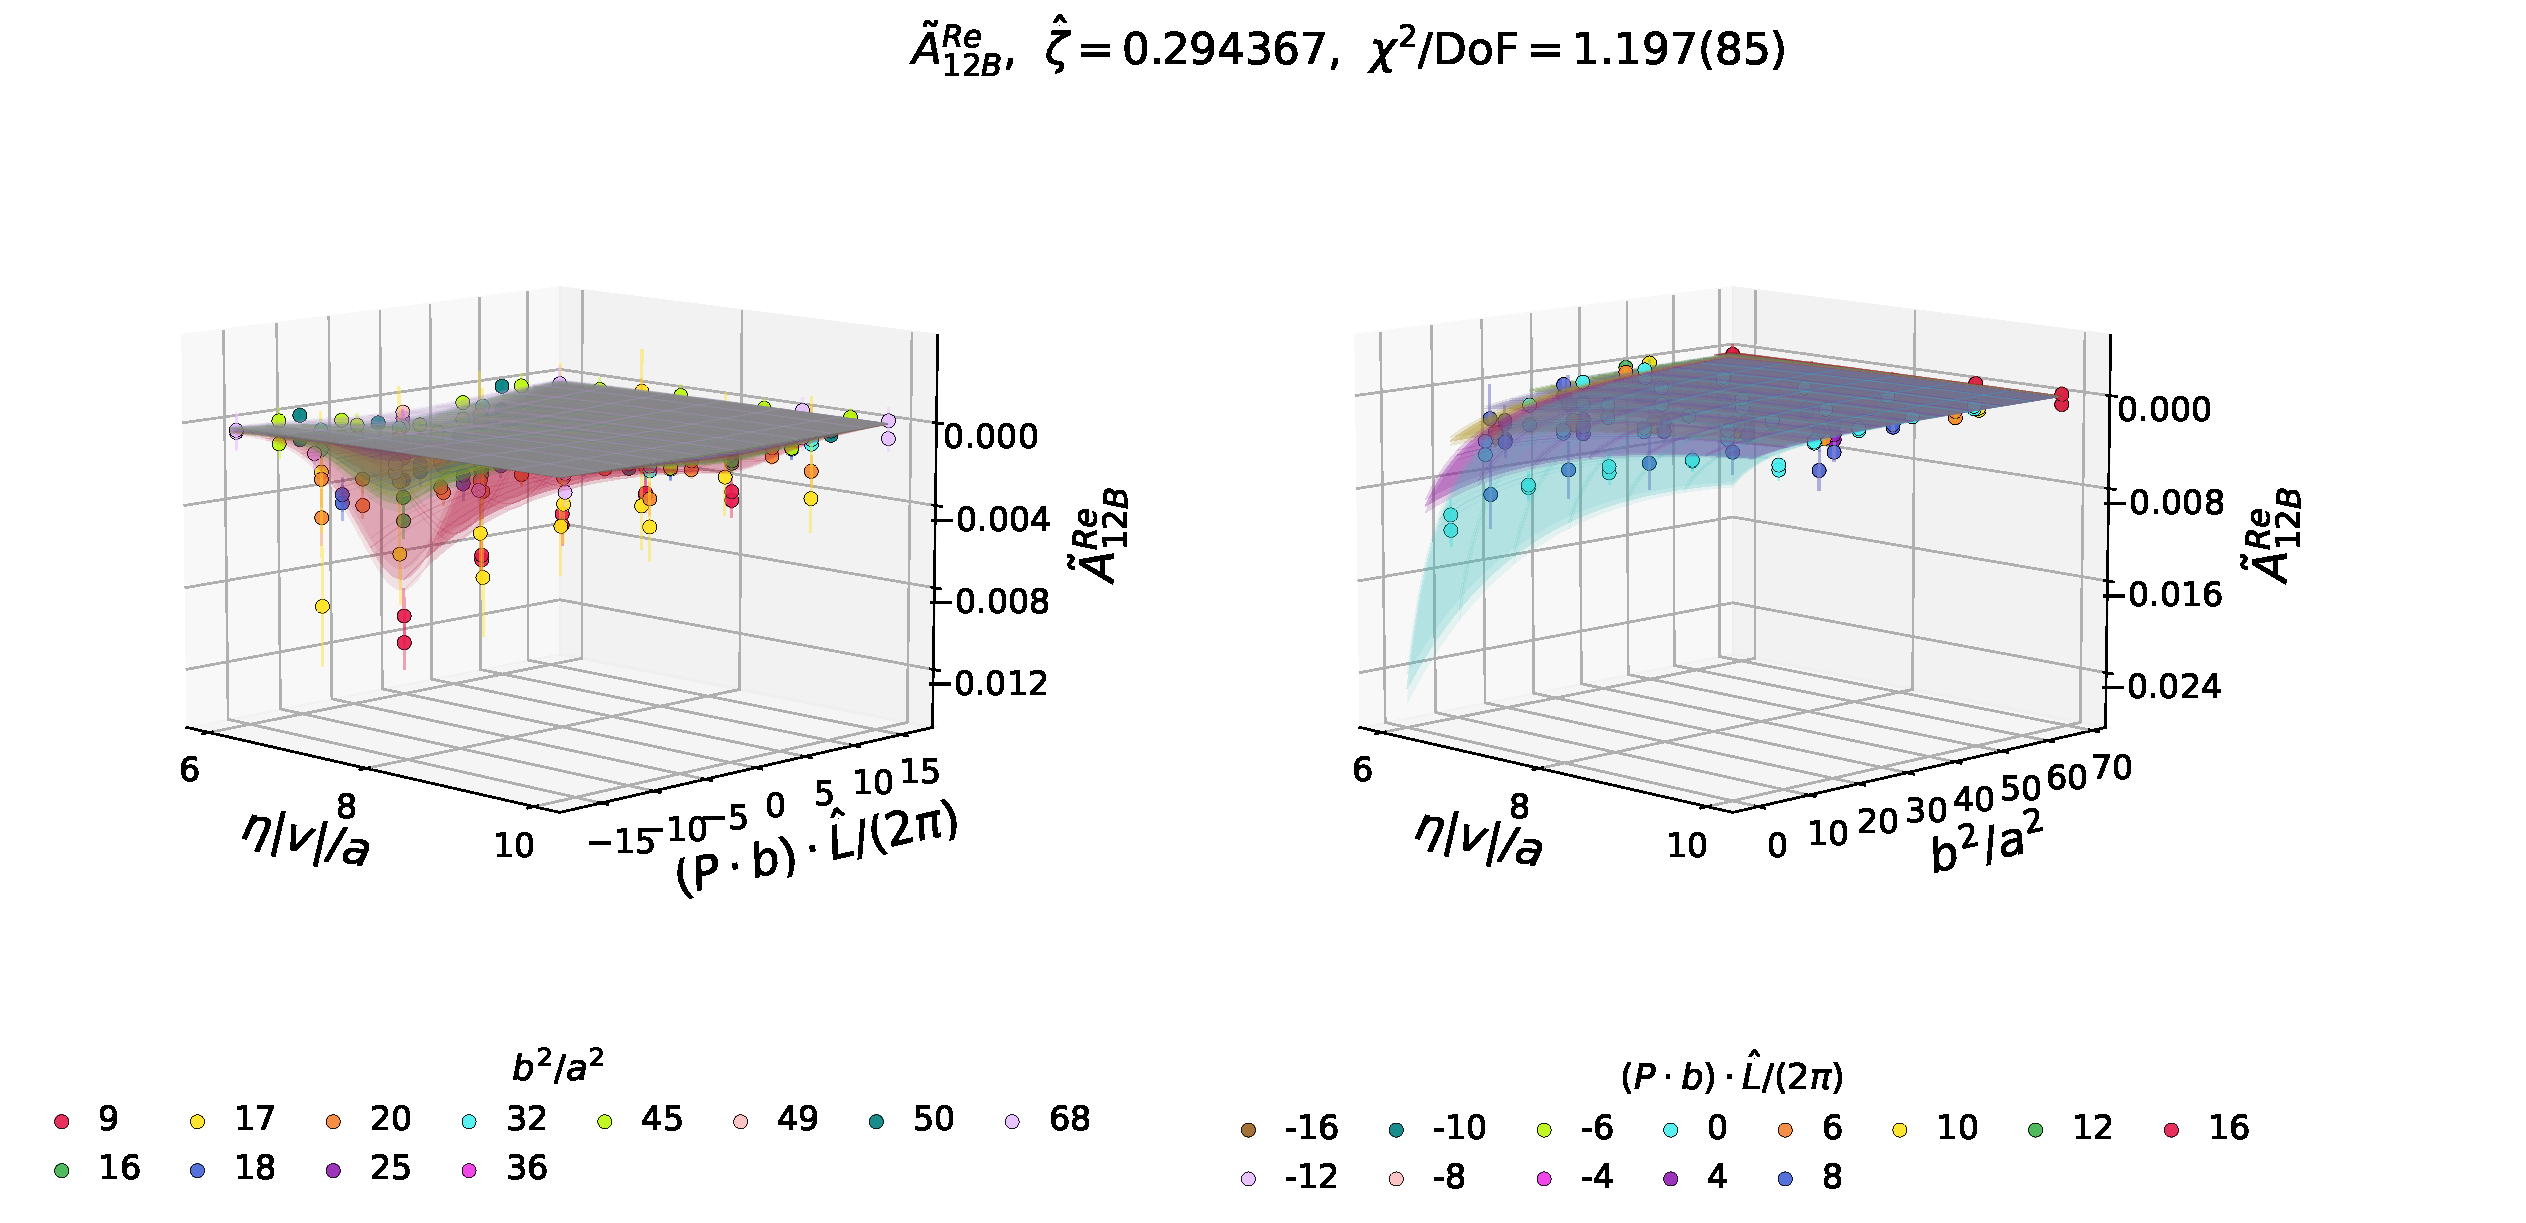
\includegraphics[width=\linewidth,height=.70\textheight,keepaspectratio]{fitting/ReA12B_Pb_bsq_PL-2_WithFit_3D.pdf}
\par\small Invariant coordinates: $(\nu,b^2,\eta)$. All panels and data overlays retained.

\figsrc{Thesis: plots; ReA12B\_Pb\_bsq\_PL-2\_WithFit\_3D}
\end{frame}

\begin{frame}{Fixed staple $\eta=8$: $\tAmp_{12B}^{\mathrm{Re}}$, $P_L=-2$}
\centering
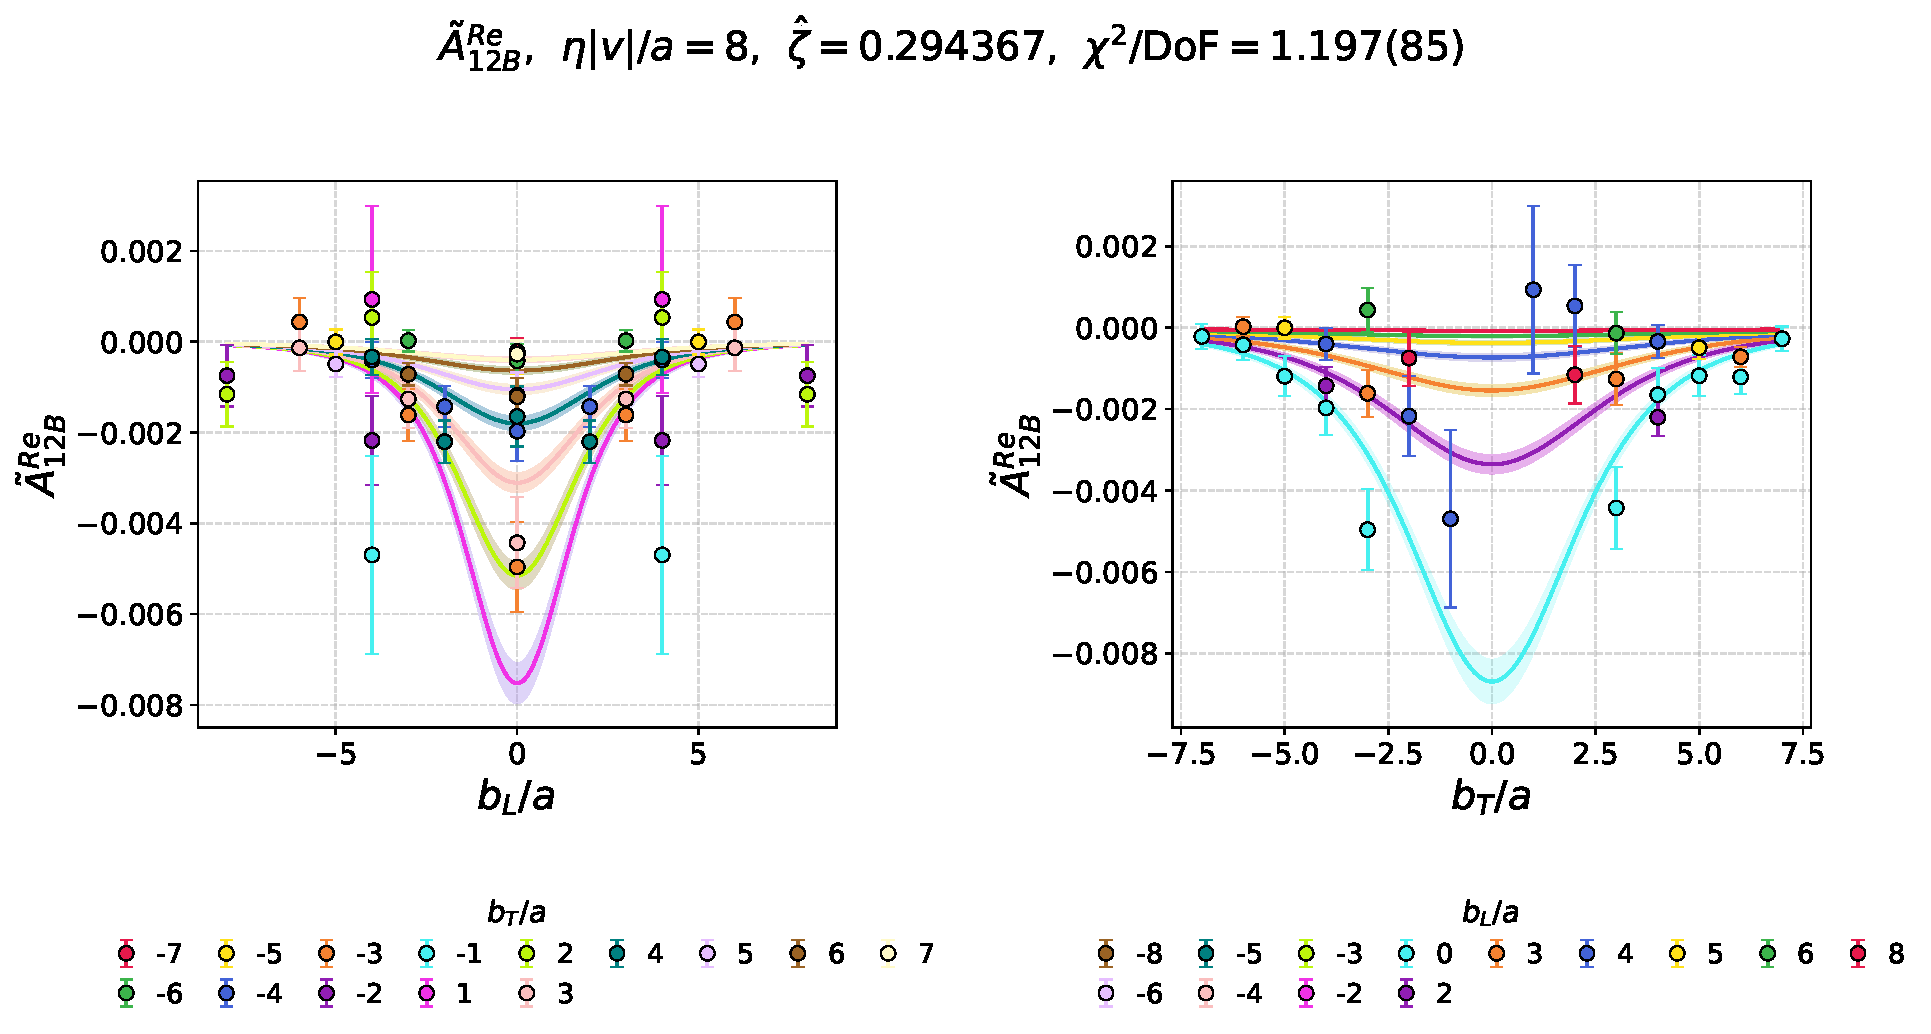
\includegraphics[width=\linewidth,height=.70\textheight,keepaspectratio]{fitting/ReA12B_eta8_PL-2_WithFit_2D.pdf}
\par\small Both spatial-coordinate slices. Same simultaneous fit, with Jackknife bands.

\figsrc{Thesis: plots; ReA12B\_eta8\_PL-2\_WithFit\_2D}
\end{frame}

\begin{frame}{Fixed staple $\eta=8$: $\tAmp_{12B}^{\mathrm{Re}}$, $P_L=-2$}
\centering
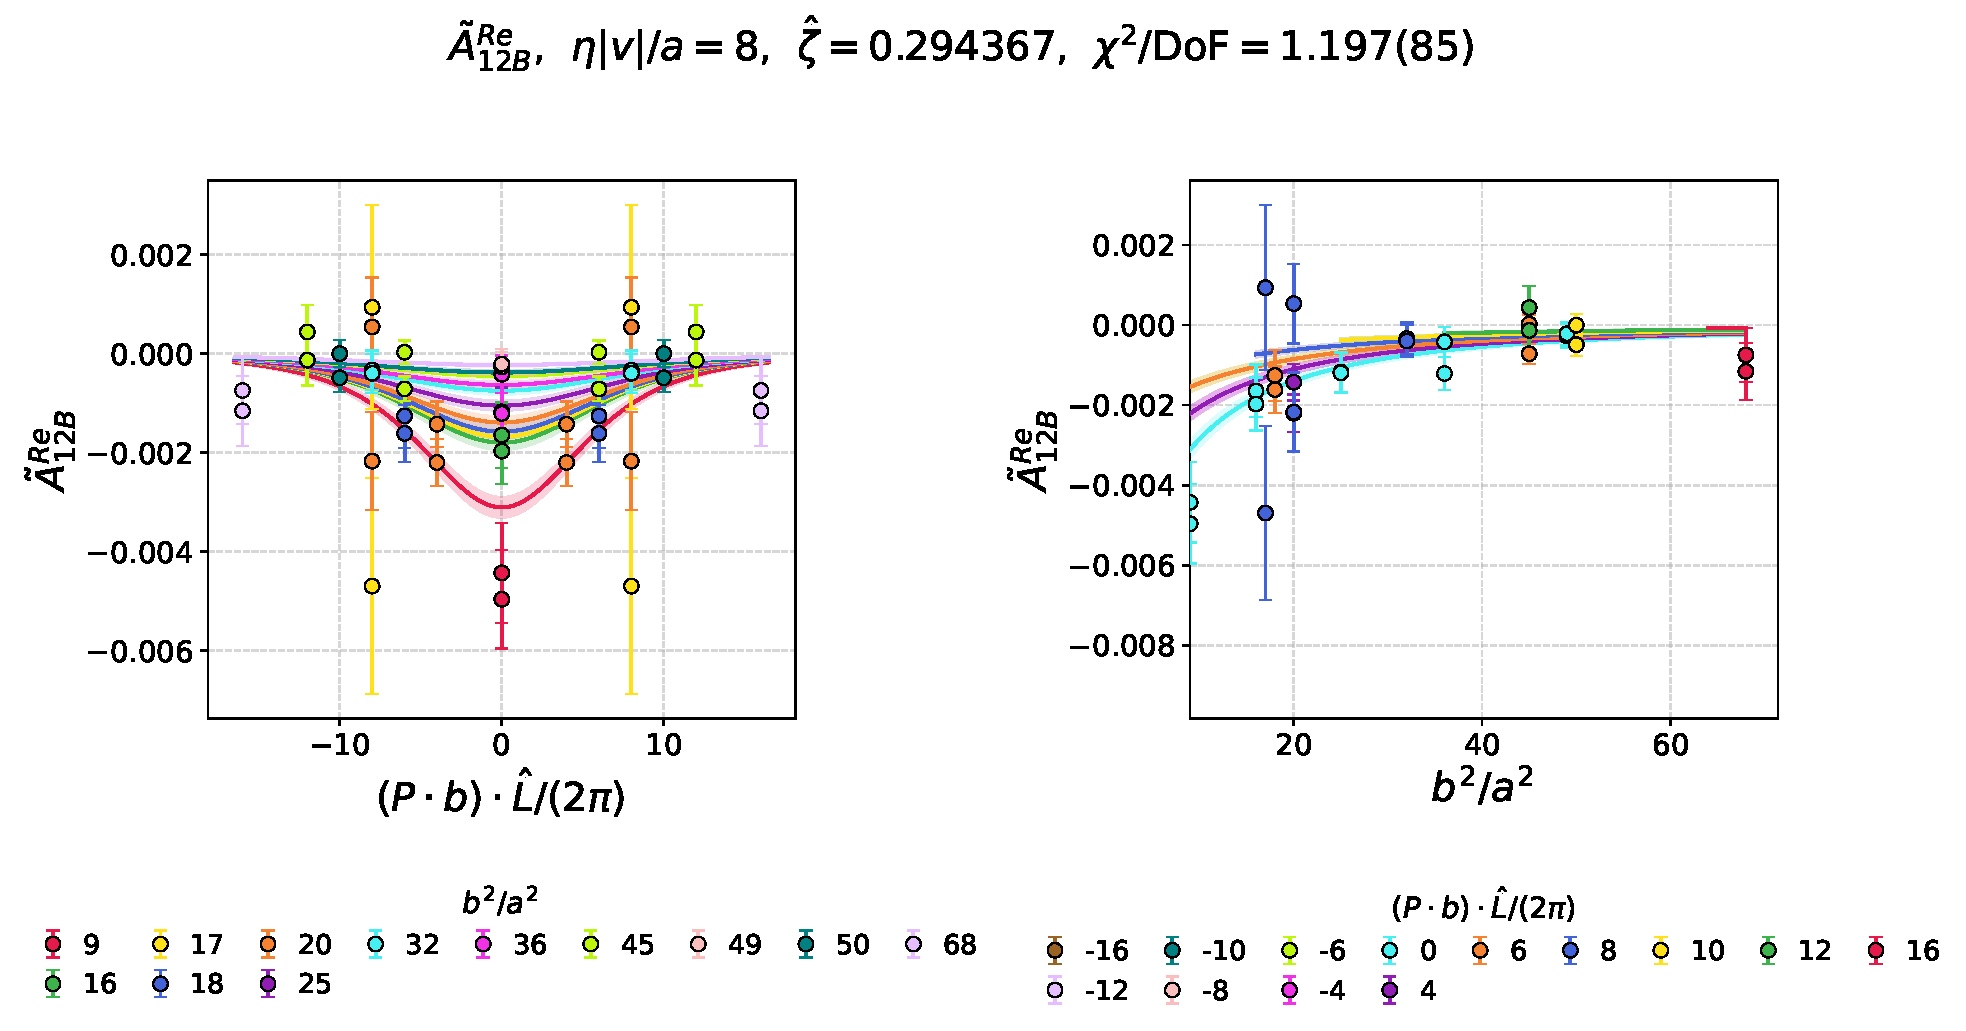
\includegraphics[width=\linewidth,height=.70\textheight,keepaspectratio]{fitting/ReA12B_Pb_bsq_eta8_PL-2_WithFit_2D.pdf}
\par\small Both invariant-coordinate slices. Same simultaneous fit, with Jackknife bands.

\figsrc{Thesis: plots; ReA12B\_Pb\_bsq\_eta8\_PL-2\_WithFit\_2D}
\end{frame}

\begin{frame}{Integrated Fourier results: $P_L=-2$}
\small\renewcommand{\arraystretch}{1.8}\begin{tabular}{lcccc}\toprule Integral & $(-\infty,\infty)$ & $[-1,1]$ & $[-1,0]$ & $[0,1]$\\\midrule
$\int dx\,E$ & 1.041(41) & 1.035(43) & 0.518(22) & 0.518(22) \\
$\int dx\,O$ & -6(176)e-17 & 7(444)e-17 & 0.257(13) & -0.257(13) \\
$\int dx\,\tilde f_1^{(0)}$ & 2.081(82) & 2.070(86) & 0.520(34) & 1.550(63) \\
$\int dx\,\tilde f_{1T}^{\perp(1)}$ & 0.451(27) & 0.451(27) & 0.225(14) & 0.225(14) \\
$m_N\int dx\,\tilde f_{1T}^{\perp(1)}/\int dx\,\tilde f_1^{(0)}$ & 0.233(14) & 0.234(14) & 0.466(36) & 0.1565(95) \\
\bottomrule\end{tabular}\par\medskip $b^2=9a^2$; all values and Jackknife uncertainties retained. Numerical values retain the source normalization. The last row is in GeV.
\figsrc{Thesis: SimultaneousFitsCov/Integration\_Table\_PL-2\_bmin3\_b2-9.tex}
\end{frame}

\begin{frame}{Fourier results (2D): $P_L=-2$, unpolarized}
\centering
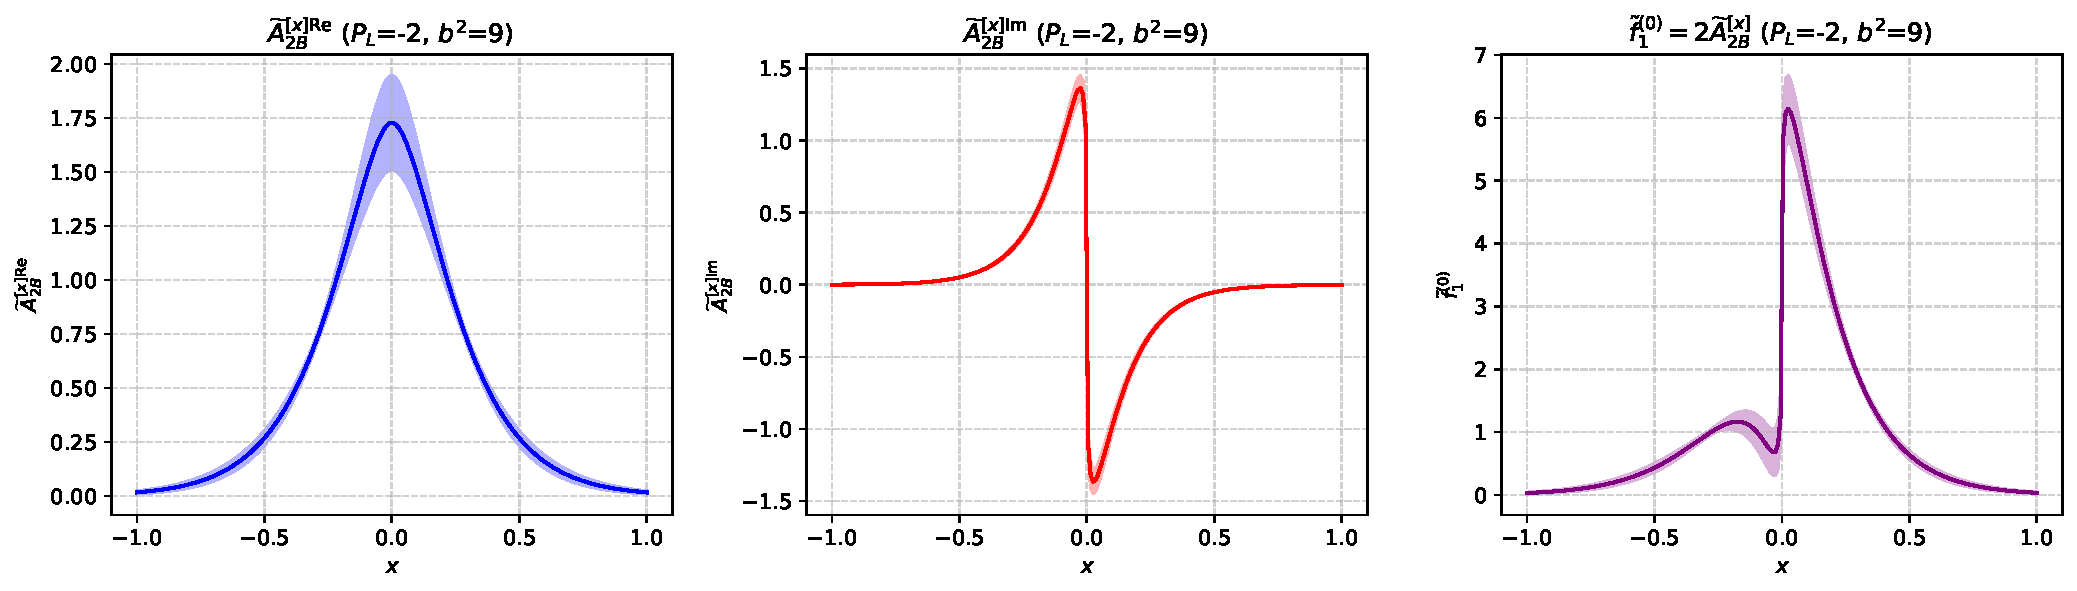
\includegraphics[width=\linewidth,height=.70\textheight,keepaspectratio]{fitting/FT_xdep_A2B_A12B_bmin3_eta610_b2-9_PL-2__row1.pdf}
\par\small Even, odd, and unpolarized transforms. Fixed $b^2=9a^2$.

\figsrc{Thesis: SimultaneousFitsCov; FT\_xdep\_A2B\_A12B\_bmin3\_eta610\_b2-9\_PL-2}
\end{frame}

\begin{frame}{Fourier results (2D): $P_L=-2$, Sivers}
\centering
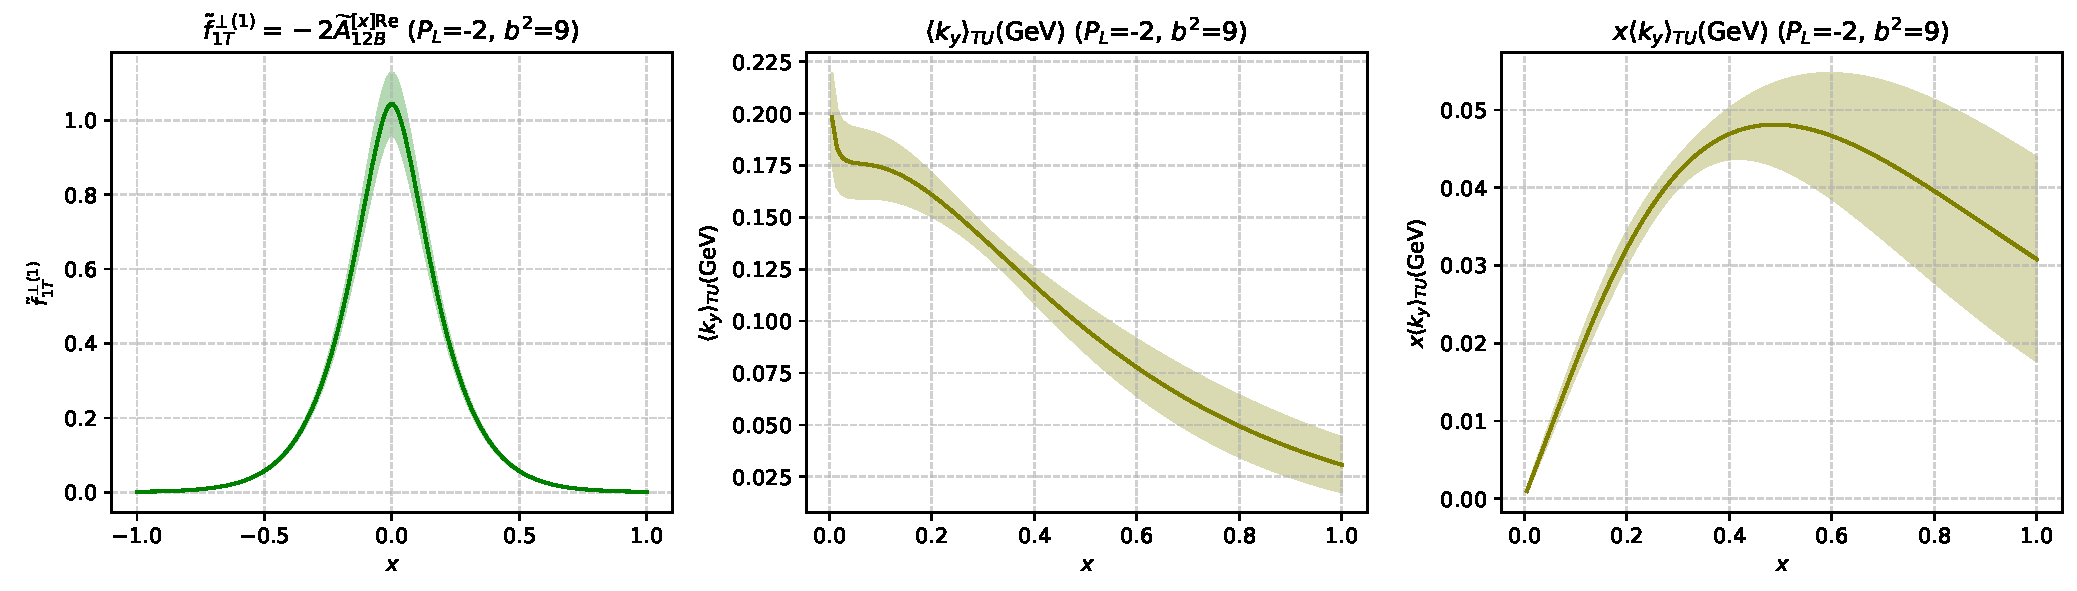
\includegraphics[width=\linewidth,height=.70\textheight,keepaspectratio]{fitting/FT_xdep_A2B_A12B_bmin3_eta610_b2-9_PL-2__row2.pdf}
\par\small Sivers transform, shift, and $x\langle k_y\rangle_{TU}$. Fixed $b^2=9a^2$.

\figsrc{Thesis: SimultaneousFitsCov; FT\_xdep\_A2B\_A12B\_bmin3\_eta610\_b2-9\_PL-2}
\end{frame}

\begin{frame}{Fourier results (3D): $P_L=-2$, unpolarized}
\centering
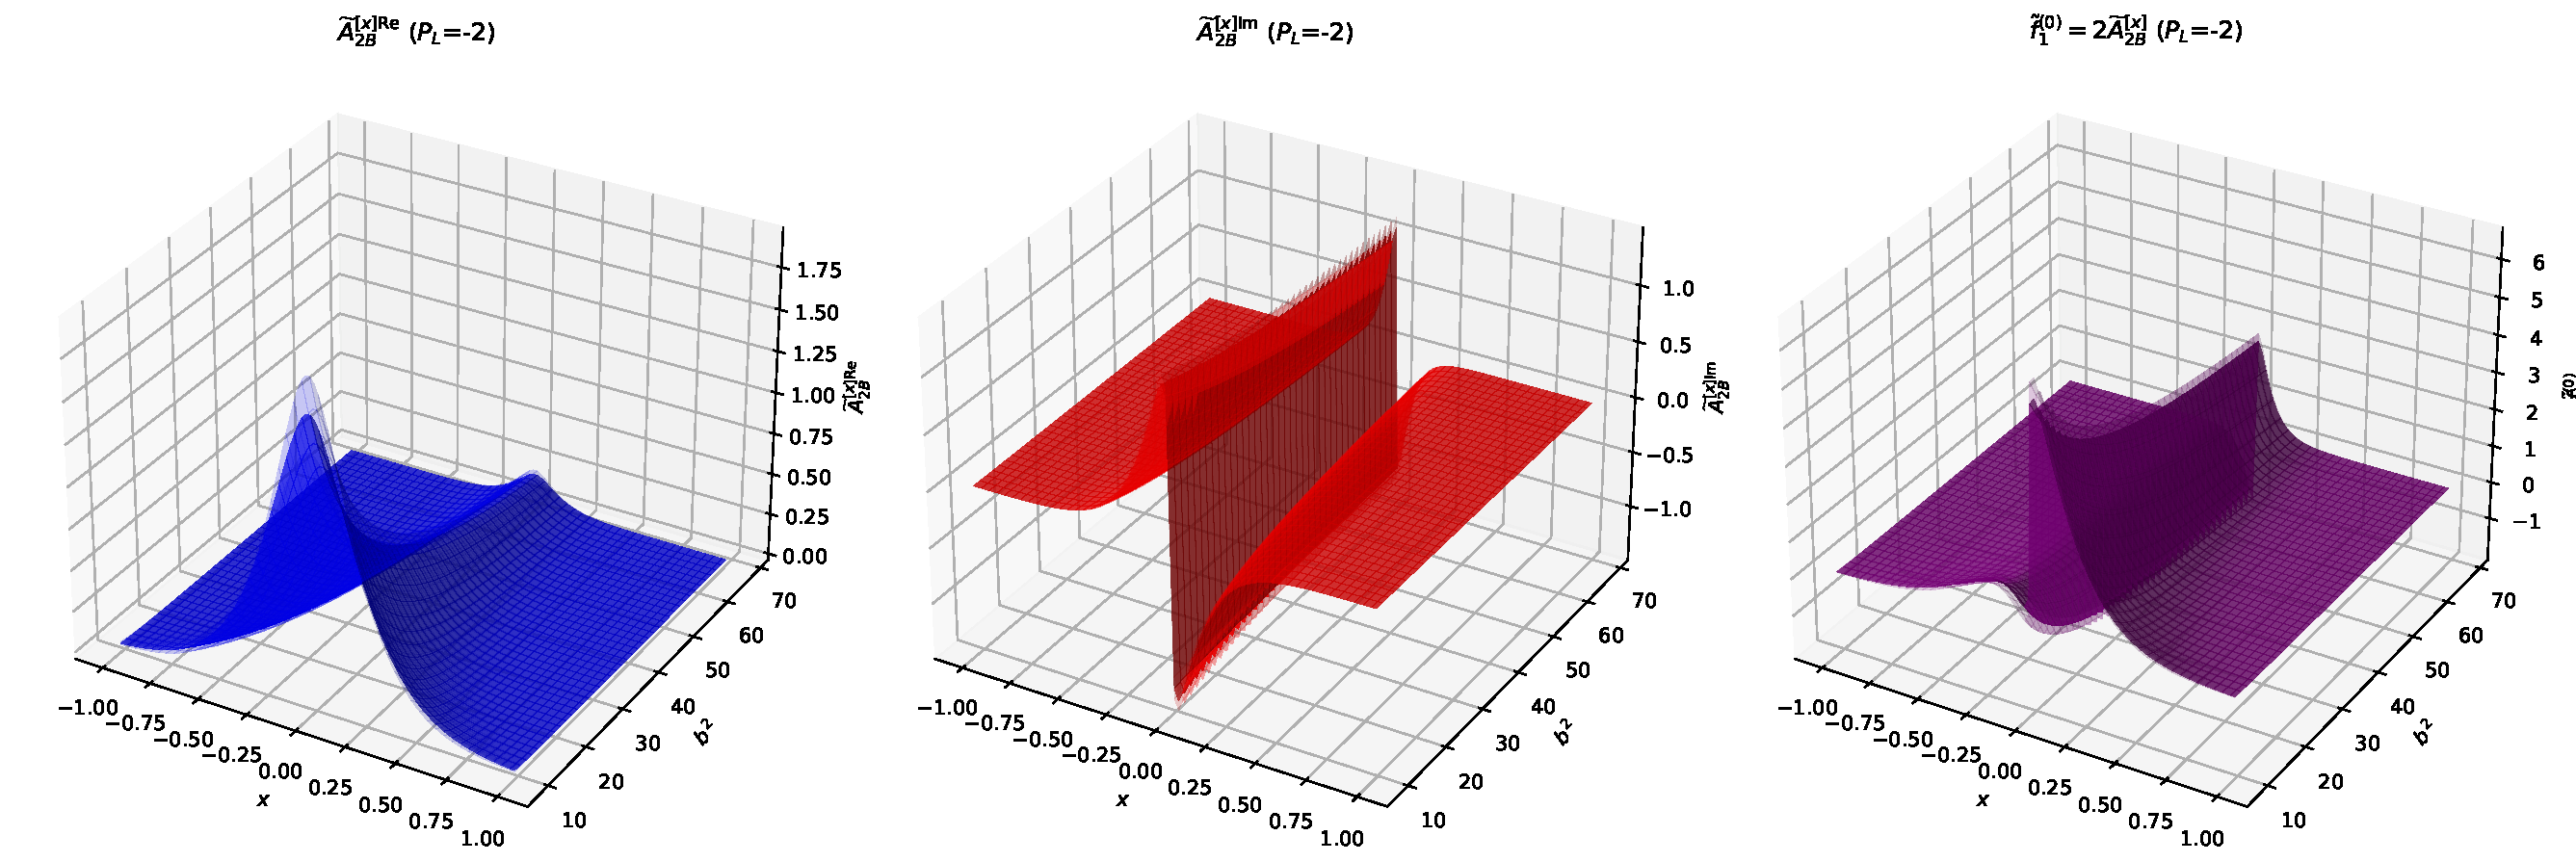
\includegraphics[width=\linewidth,height=.70\textheight,keepaspectratio]{fitting/FT_xdep_3D_A2B_A12B_bmin3_eta610_PL-2__row1.pdf}
\par\small Even, odd, and unpolarized transforms. Full $b^2/a^2\in[9,68]$ dependence.

\figsrc{Thesis: SimultaneousFitsCov; FT\_xdep\_3D\_A2B\_A12B\_bmin3\_eta610\_PL-2}
\end{frame}

\begin{frame}{Fourier results (3D): $P_L=-2$, Sivers}
\centering
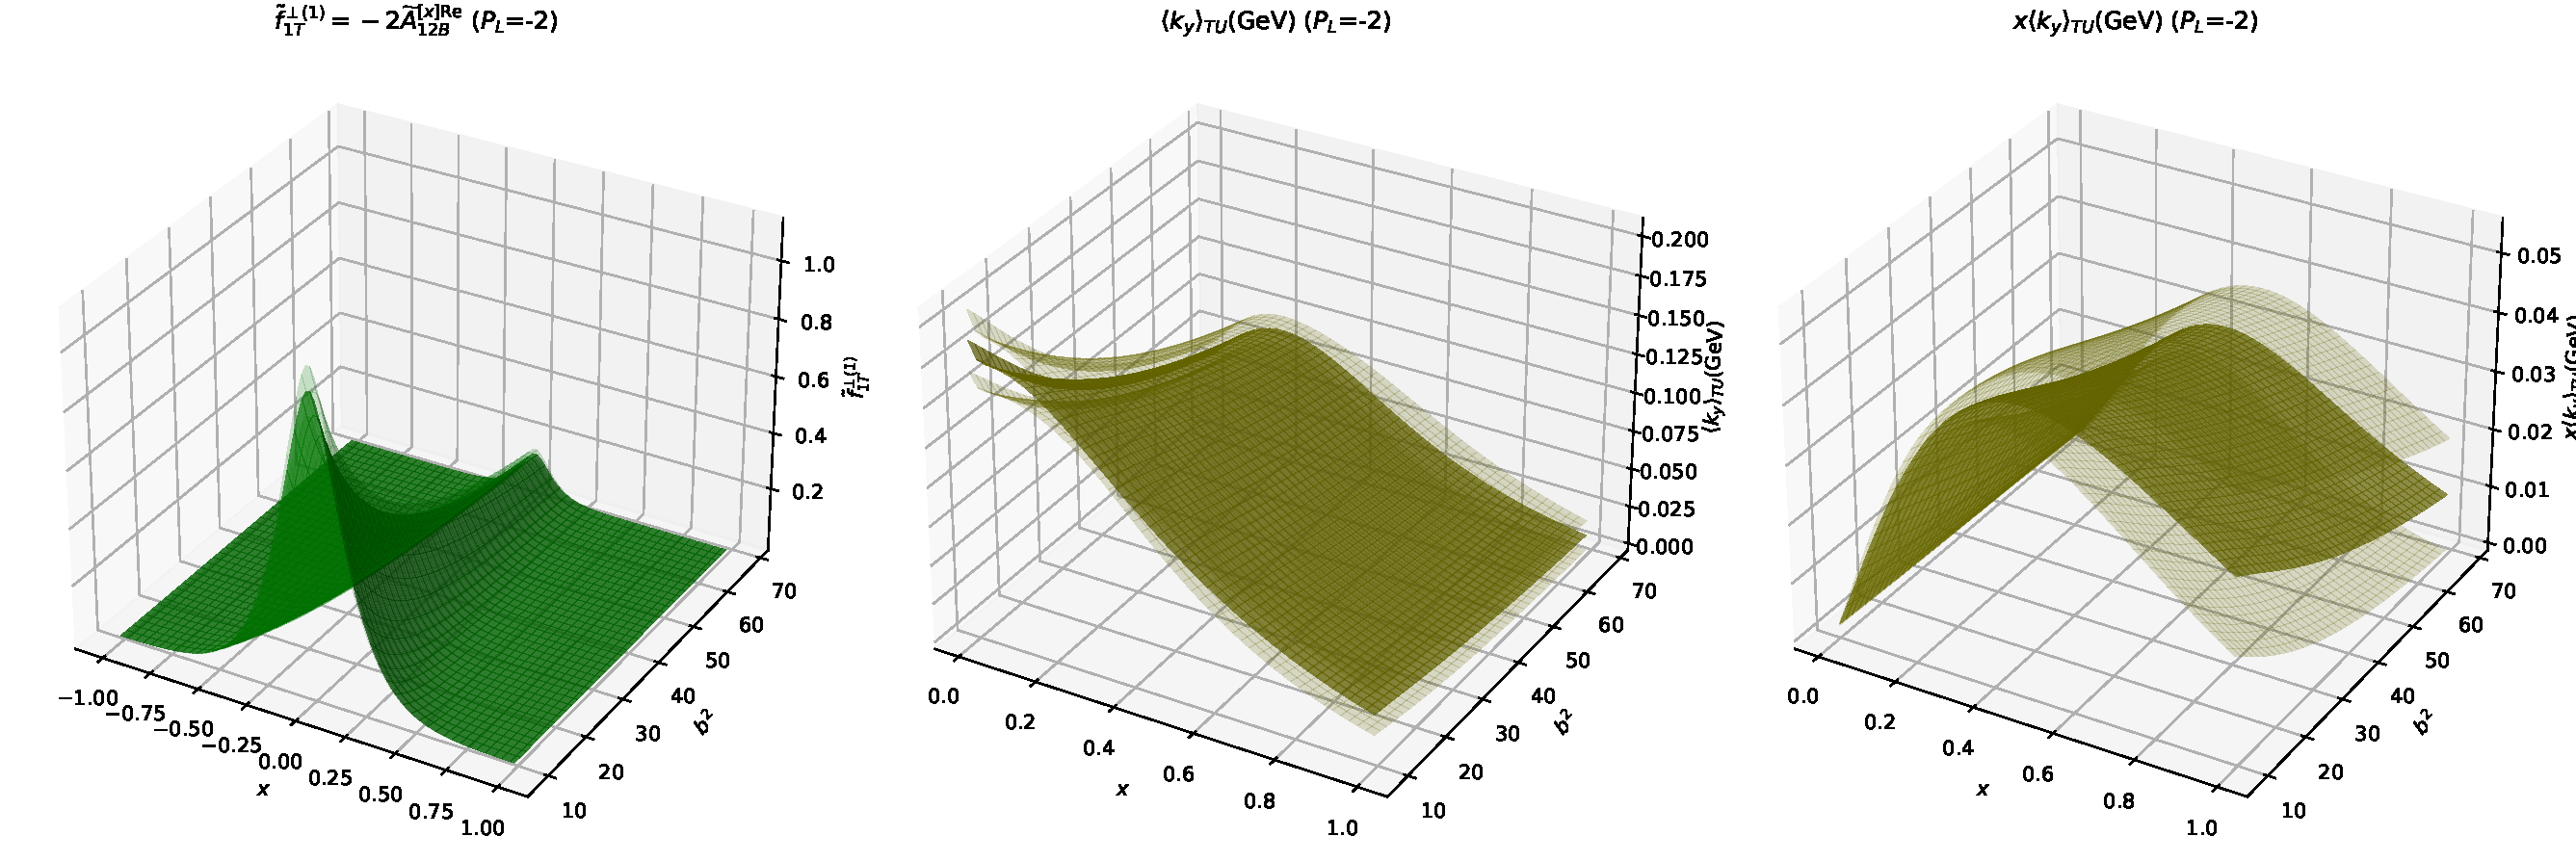
\includegraphics[width=\linewidth,height=.70\textheight,keepaspectratio]{fitting/FT_xdep_3D_A2B_A12B_bmin3_eta610_PL-2__row2.pdf}
\par\small Sivers transform, shift, and $x\langle k_y\rangle_{TU}$. Full $b^2/a^2\in[9,68]$ dependence.

\figsrc{Thesis: SimultaneousFitsCov; FT\_xdep\_3D\_A2B\_A12B\_bmin3\_eta610\_PL-2}
\end{frame}

\begin{frame}{Simultaneous fit parameters: $P_L=-3$}
\small $|\vect b|\ge3a$, $6\le\eta\le10$; reported $\chi^2_{\rm aug}/N_{\rm data}=0.712(66)$.\par\medskip
\begin{columns}[t]\begin{column}{.32\textwidth}\centering $\tAmp_{2B}^{\mathrm{Re}}$\par\medskip\renewcommand{\arraystretch}{1.3}\begin{tabular}{cc}\toprule Parameter & Value\\\midrule
$a$ & $4.0061(31)$ \\
$c$ & $0.45(12)$ \\
$d$ & $0.136(11)$ \\
$k_1$ & $12.284(11)$ \\
$k_2$ & $-36.1973(19)$ \\
$j$ & $2.085(10)$ \\
$f$ & $0.540(15)$ \\\bottomrule\end{tabular}\end{column}\begin{column}{.32\textwidth}\centering $\tAmp_{2B}^{\mathrm{Im}}$\par\medskip\renewcommand{\arraystretch}{1.3}\begin{tabular}{cc}\toprule Parameter & Value\\\midrule
$a''$ & $0.328(11)$ \\
$c''$ & $0.163(15)$ \\
$d''$ & $0.147(13)$ \\
$j''$ & $1.057(15)$ \\
$f$ & $0.540(15)$ \\\bottomrule\end{tabular}\end{column}\begin{column}{.32\textwidth}\centering $\tAmp_{12B}^{\mathrm{Re}}$\par\medskip\renewcommand{\arraystretch}{1.3}\begin{tabular}{cc}\toprule Parameter & Value\\\midrule
$a'$ & $0.569(13)$ \\
$c'$ & $0.100(17)$ \\
$d'$ & $0.094(16)$ \\
$j'$ & $1.9969(49)$ \\
$f$ & $0.540(15)$ \\\bottomrule\end{tabular}\end{column}\end{columns}
\figsrc{Thesis: SimultaneousFitsCov/Fit\_Table\_PL-3\_bmin3.tex}
\end{frame}

\begin{frame}{Global fit: $\tAmp_{2B}^{\mathrm{Re}}$, $P_L=-3$}
\centering
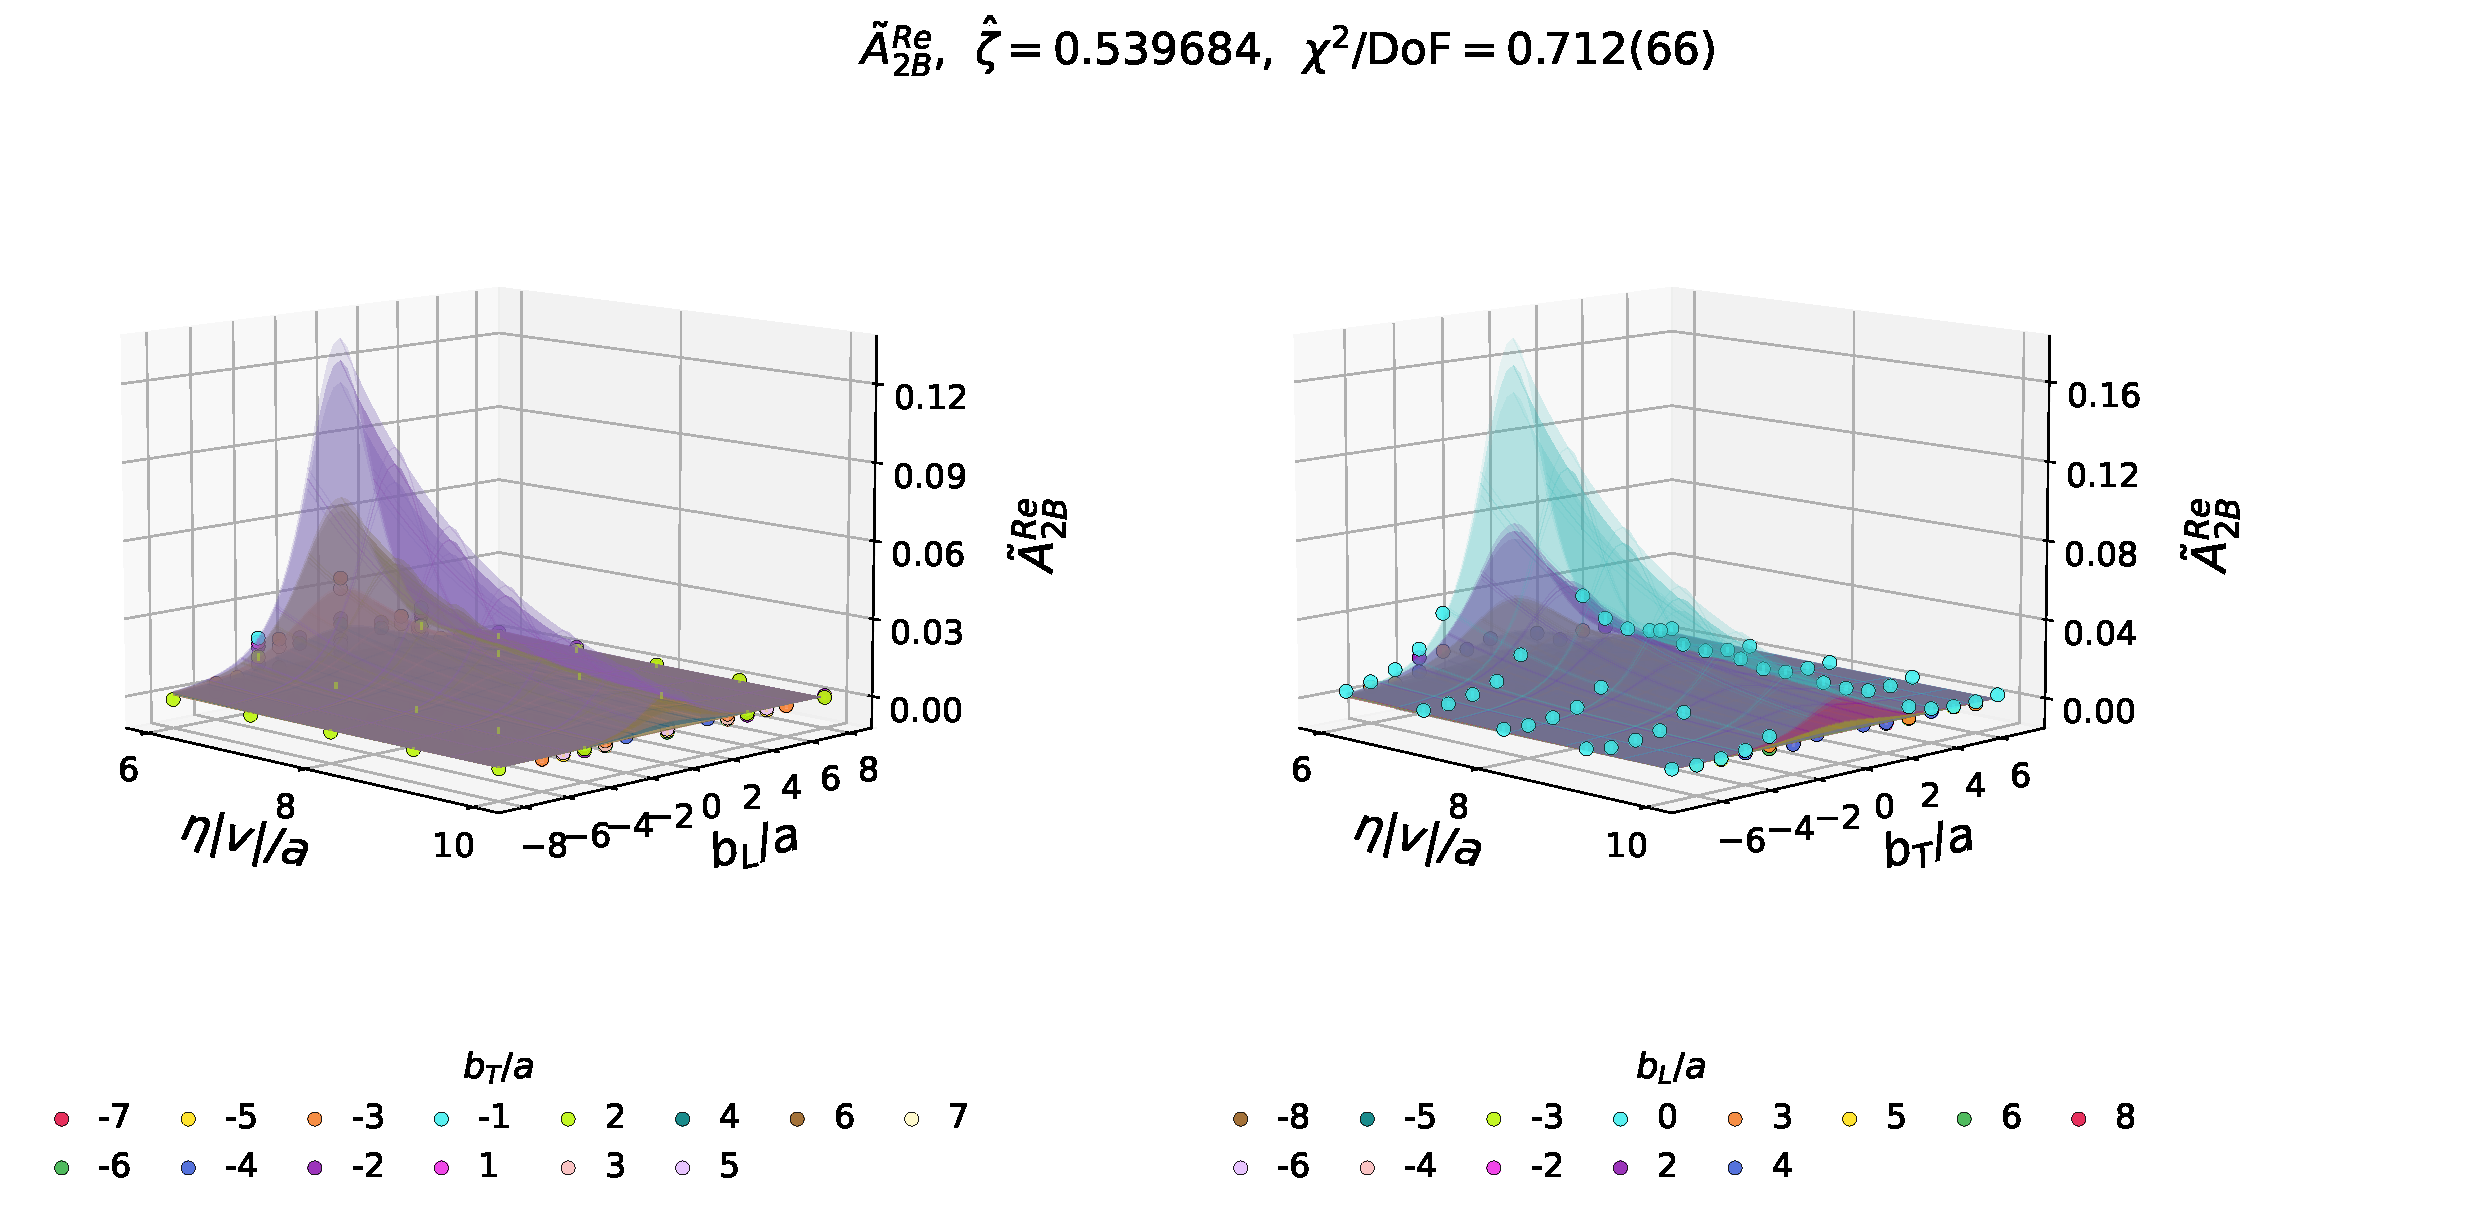
\includegraphics[width=\linewidth,height=.70\textheight,keepaspectratio]{fitting/ReA2B_PL-3_WithFit_3D.pdf}
\par\small Spatial coordinates: $(b_L,b_T,\eta)$. All panels and data overlays retained.

\figsrc{Thesis: plots; ReA2B\_PL-3\_WithFit\_3D}
\end{frame}

\begin{frame}{Global fit: $\tAmp_{2B}^{\mathrm{Re}}$, $P_L=-3$}
\centering
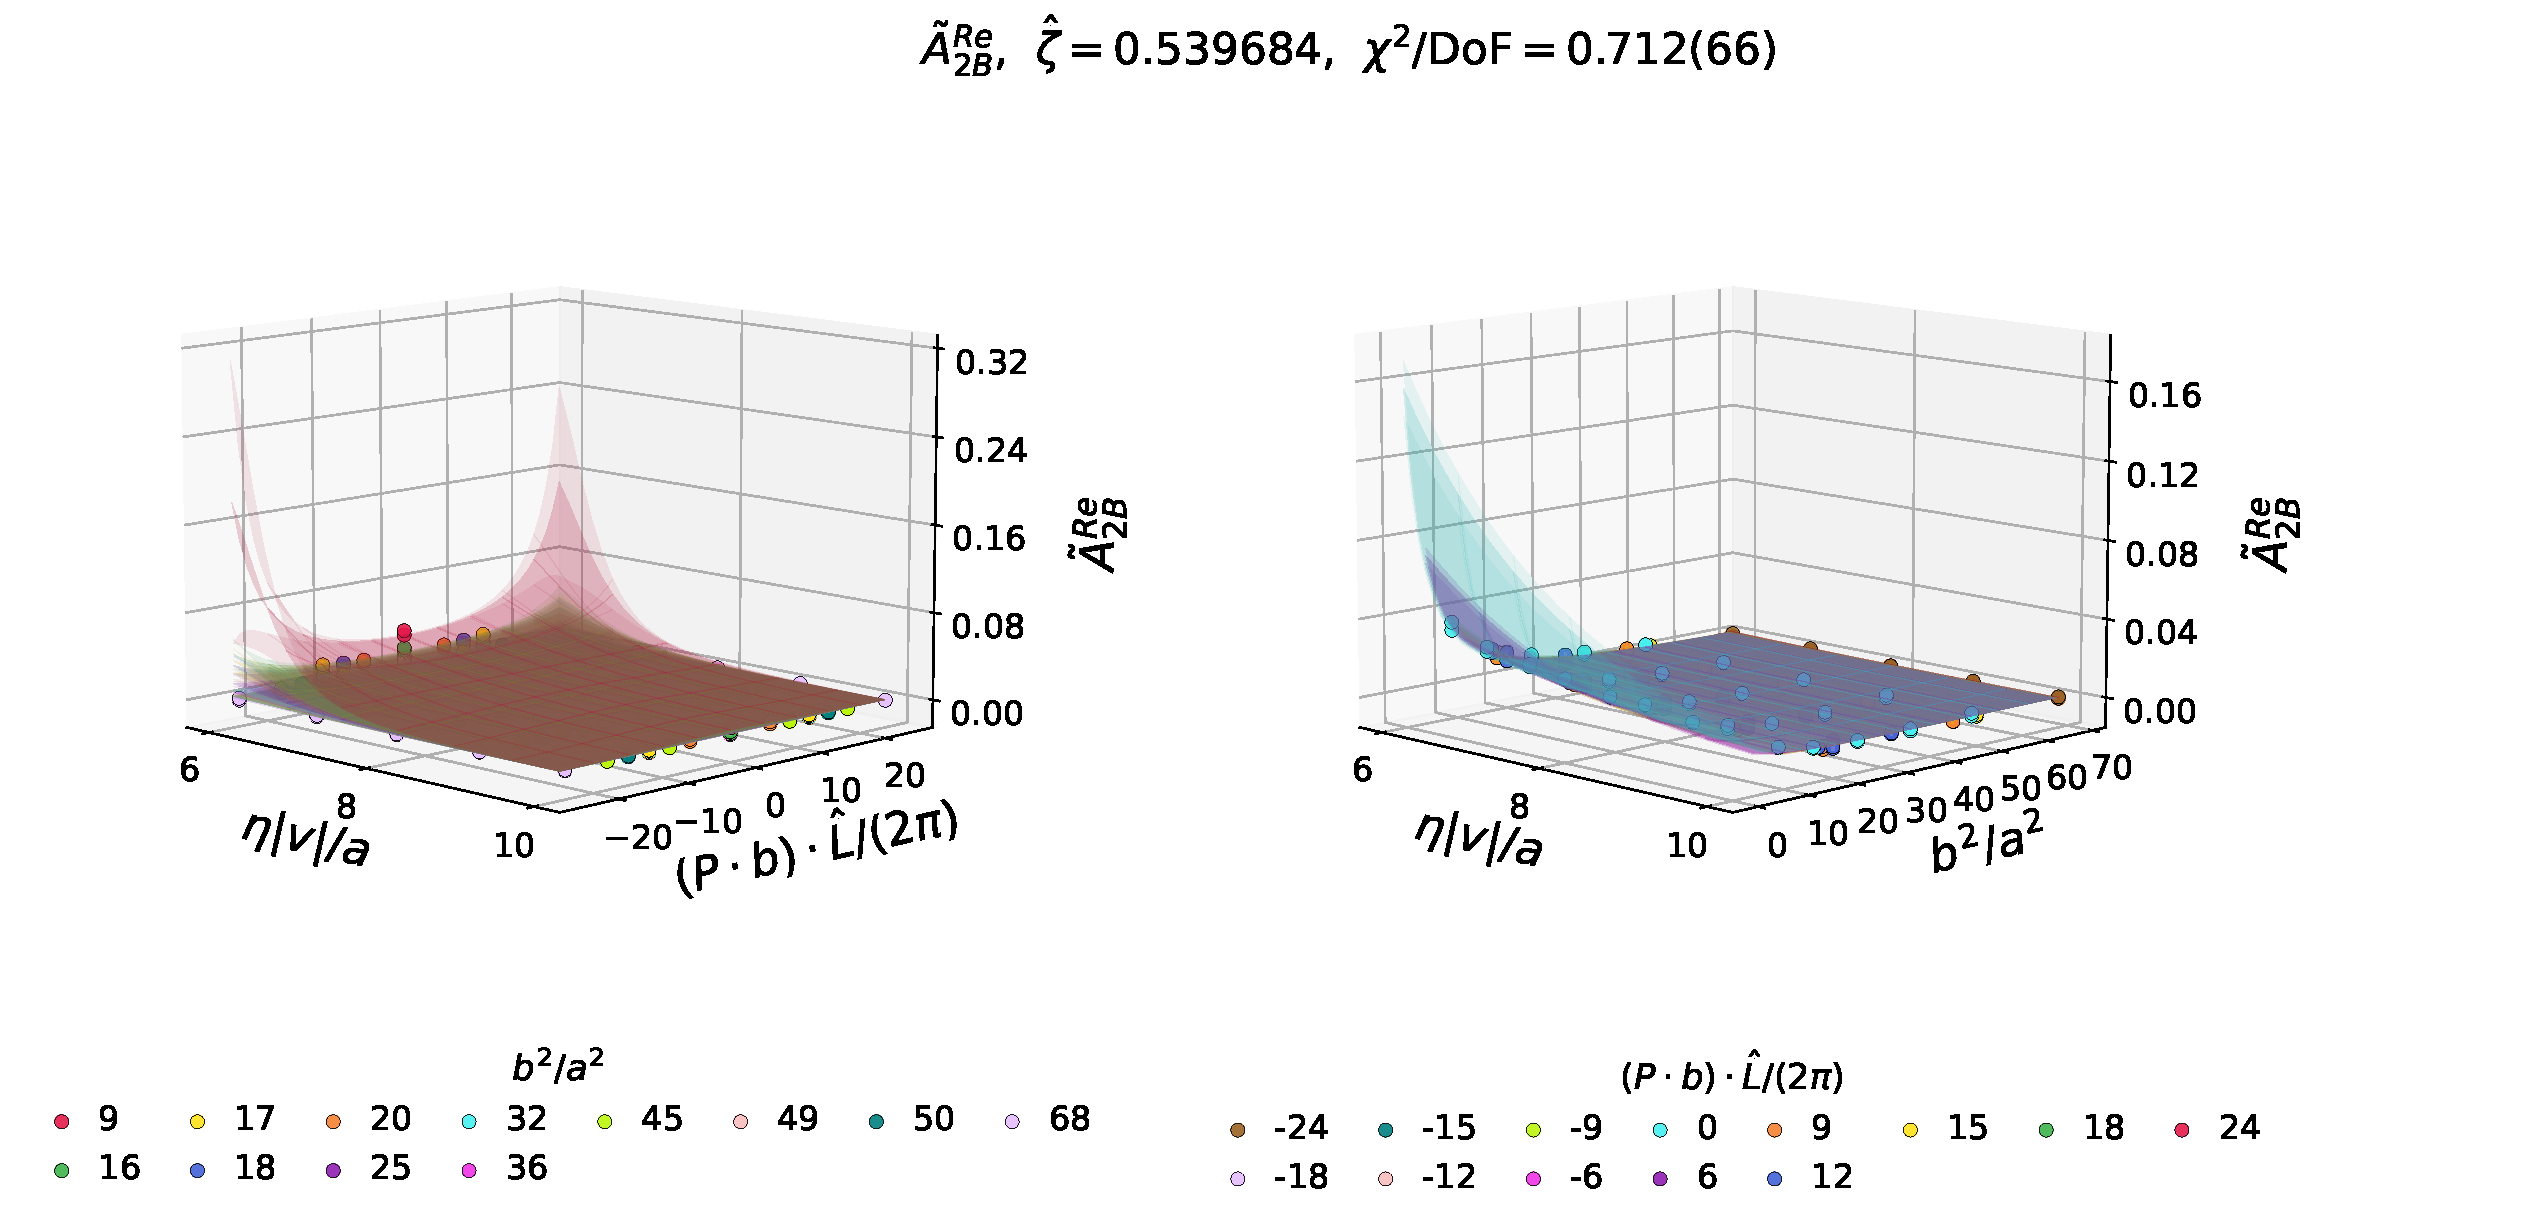
\includegraphics[width=\linewidth,height=.70\textheight,keepaspectratio]{fitting/ReA2B_Pb_bsq_PL-3_WithFit_3D.pdf}
\par\small Invariant coordinates: $(\nu,b^2,\eta)$. All panels and data overlays retained.

\figsrc{Thesis: plots; ReA2B\_Pb\_bsq\_PL-3\_WithFit\_3D}
\end{frame}

\begin{frame}{Fixed staple $\eta=8$: $\tAmp_{2B}^{\mathrm{Re}}$, $P_L=-3$}
\centering
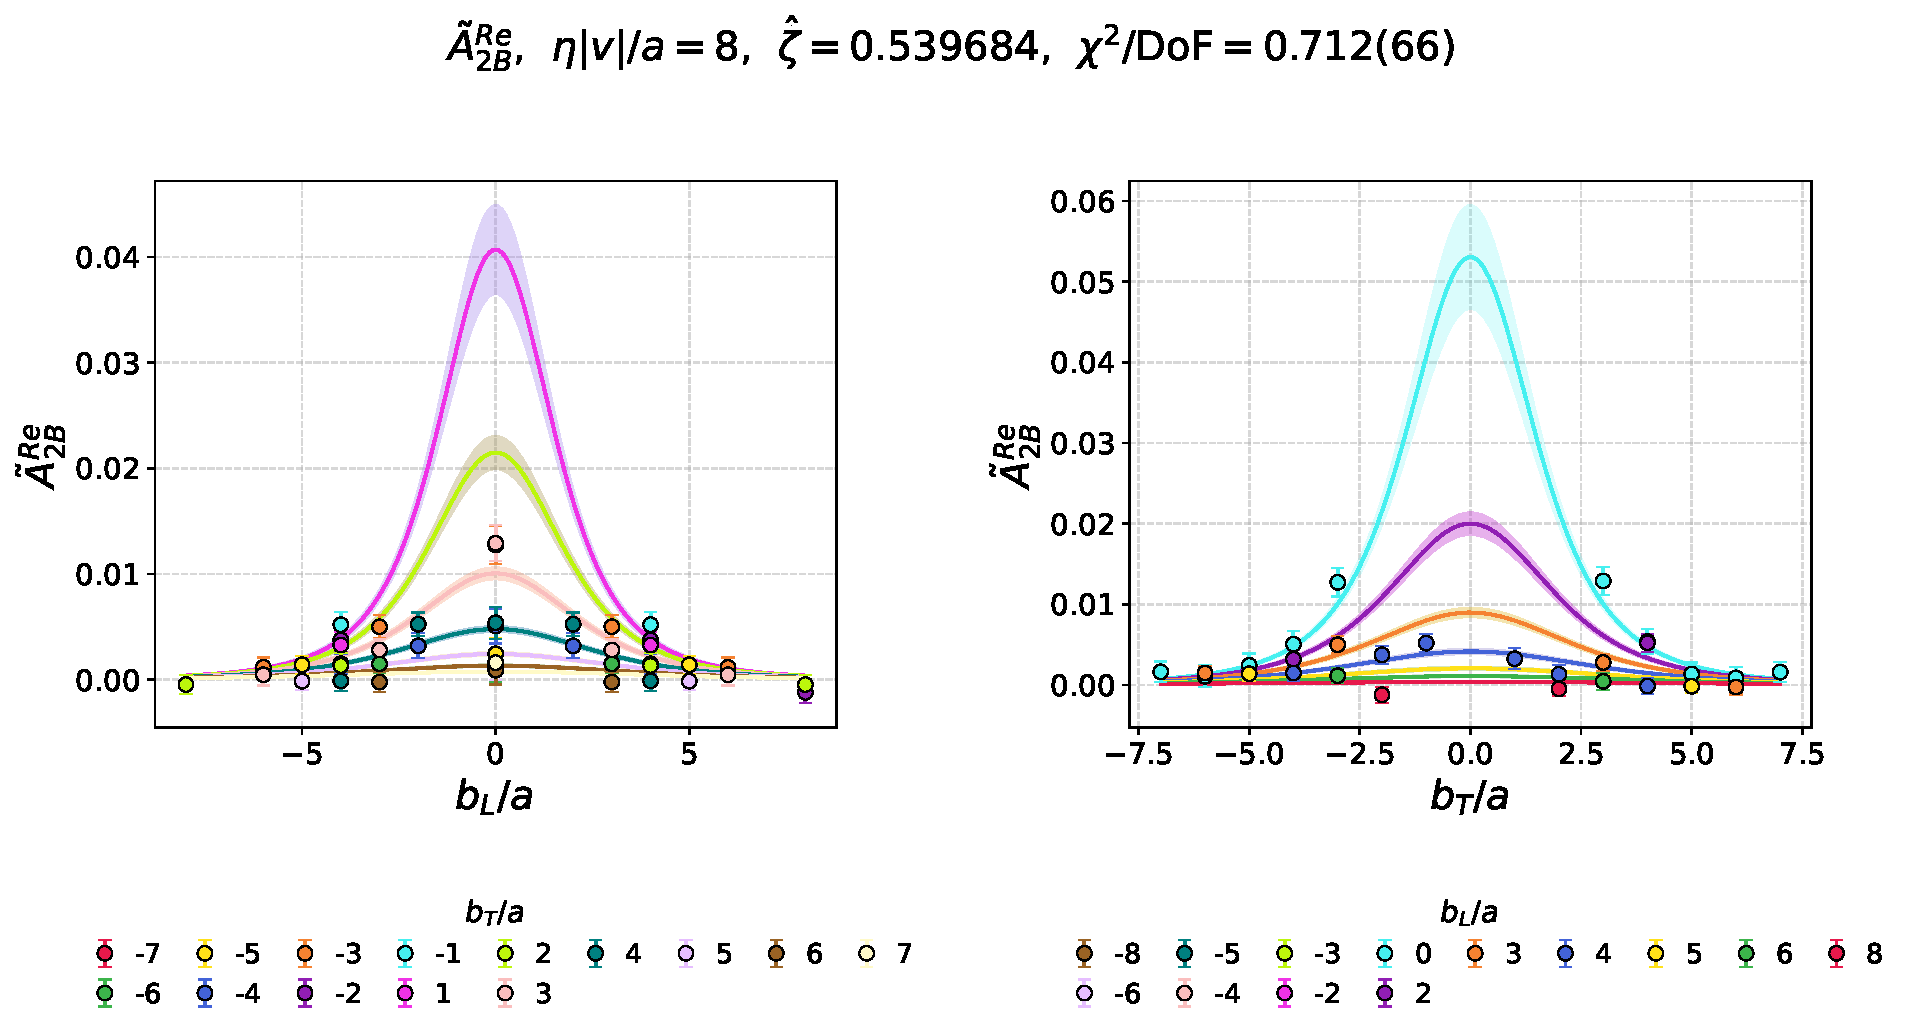
\includegraphics[width=\linewidth,height=.70\textheight,keepaspectratio]{fitting/ReA2B_eta8_PL-3_WithFit_2D.pdf}
\par\small Both spatial-coordinate slices. Same simultaneous fit, with Jackknife bands.

\figsrc{Thesis: plots; ReA2B\_eta8\_PL-3\_WithFit\_2D}
\end{frame}

\begin{frame}{Fixed staple $\eta=8$: $\tAmp_{2B}^{\mathrm{Re}}$, $P_L=-3$}
\centering
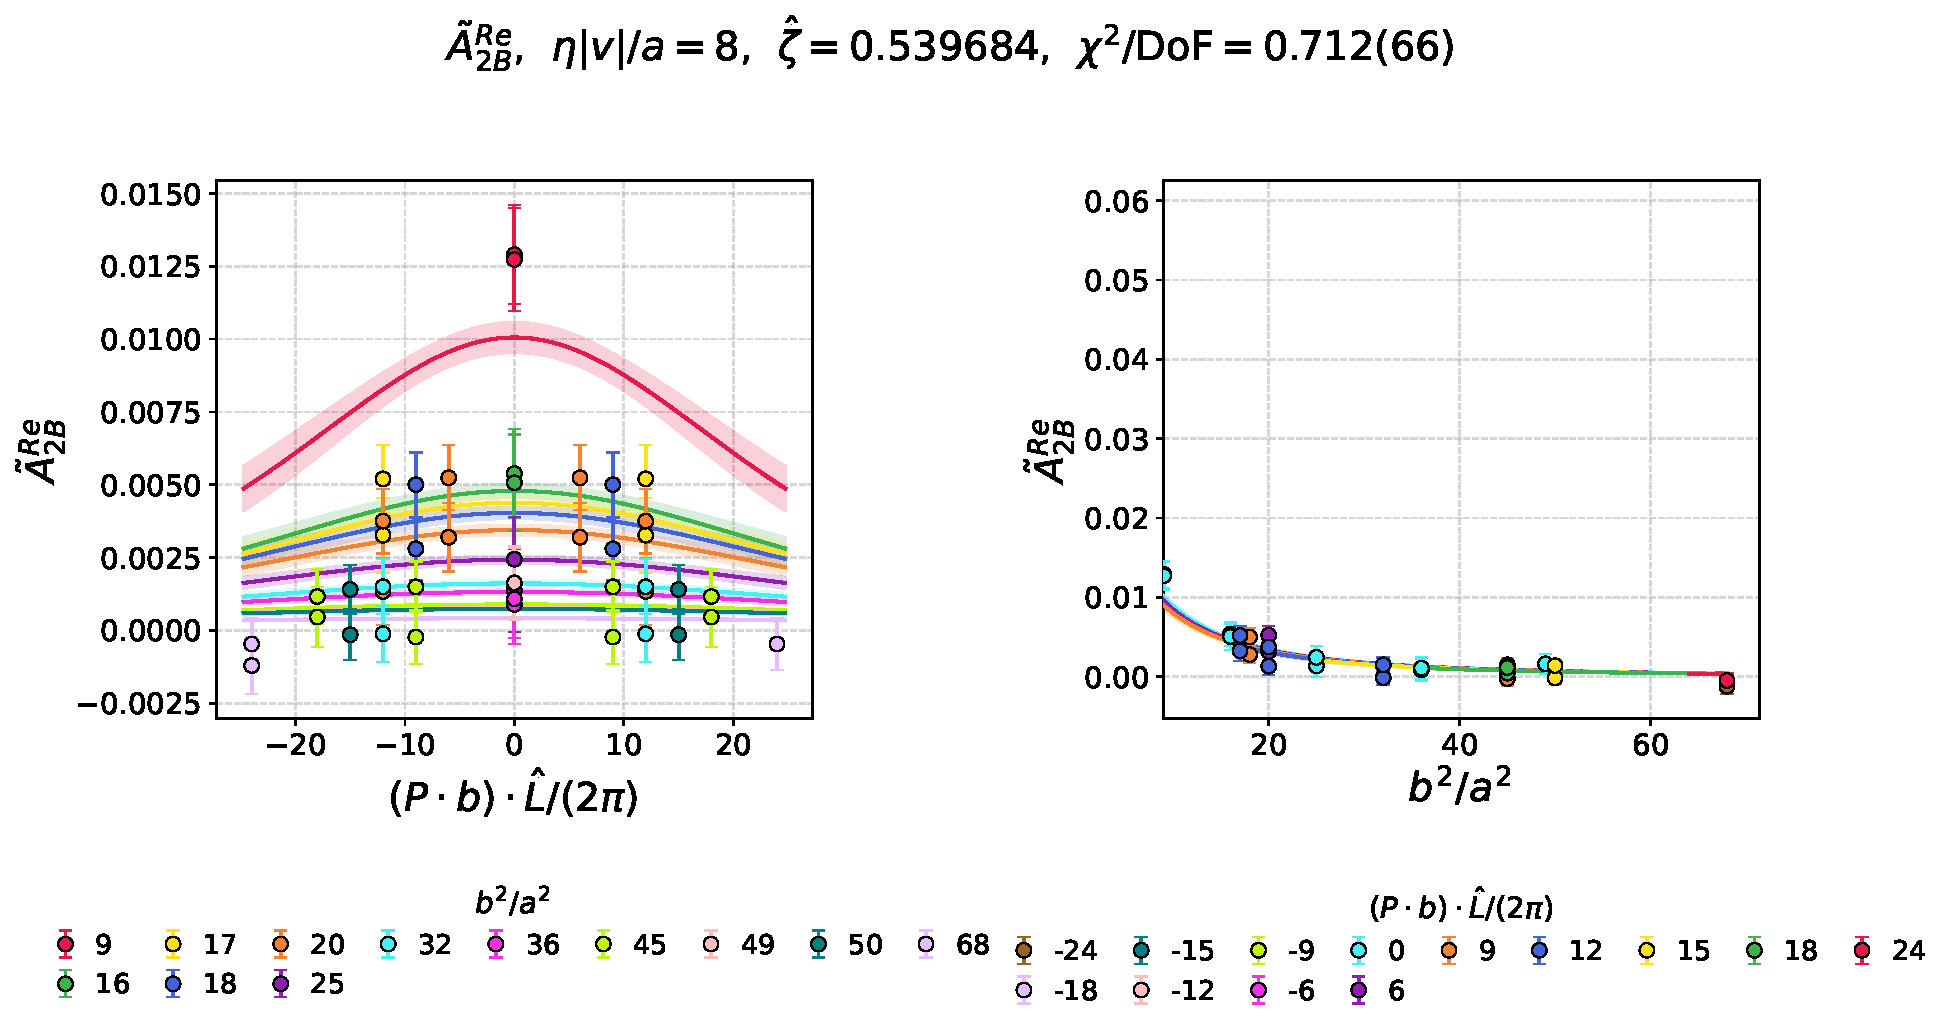
\includegraphics[width=\linewidth,height=.70\textheight,keepaspectratio]{fitting/ReA2B_Pb_bsq_eta8_PL-3_WithFit_2D.pdf}
\par\small Both invariant-coordinate slices. Same simultaneous fit, with Jackknife bands.

\figsrc{Thesis: plots; ReA2B\_Pb\_bsq\_eta8\_PL-3\_WithFit\_2D}
\end{frame}

\begin{frame}{Global fit: $\tAmp_{2B}^{\mathrm{Im}}$, $P_L=-3$}
\centering
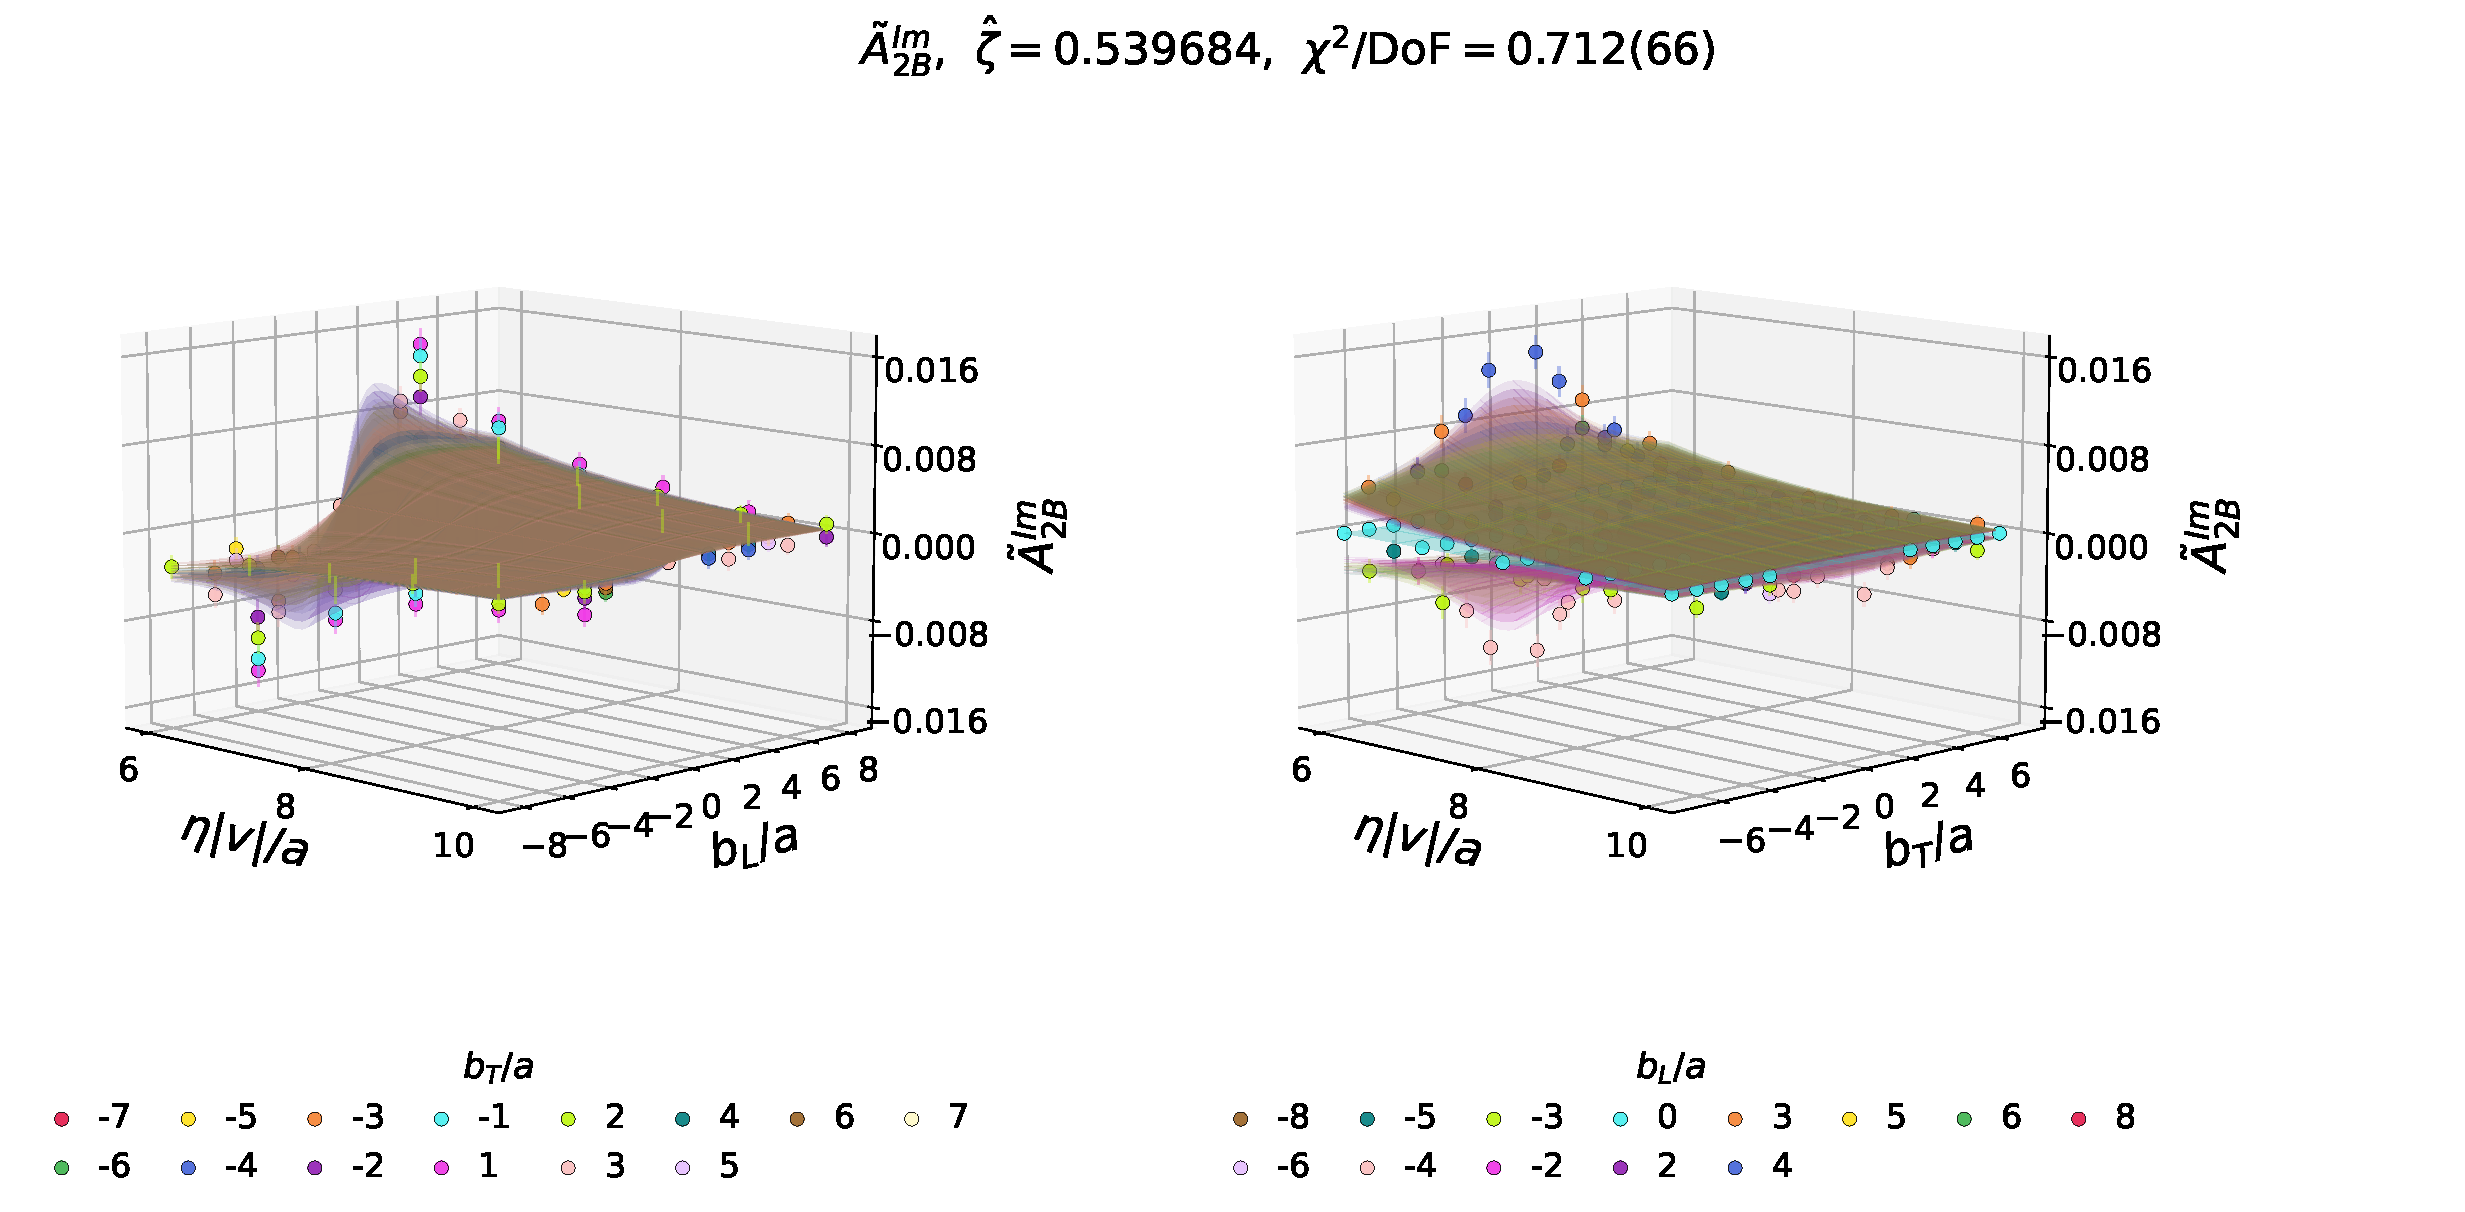
\includegraphics[width=\linewidth,height=.70\textheight,keepaspectratio]{fitting/ImA2B_PL-3_WithFit_3D.pdf}
\par\small Spatial coordinates: $(b_L,b_T,\eta)$. All panels and data overlays retained.

\figsrc{Thesis: plots; ImA2B\_PL-3\_WithFit\_3D}
\end{frame}

\begin{frame}{Global fit: $\tAmp_{2B}^{\mathrm{Im}}$, $P_L=-3$}
\centering
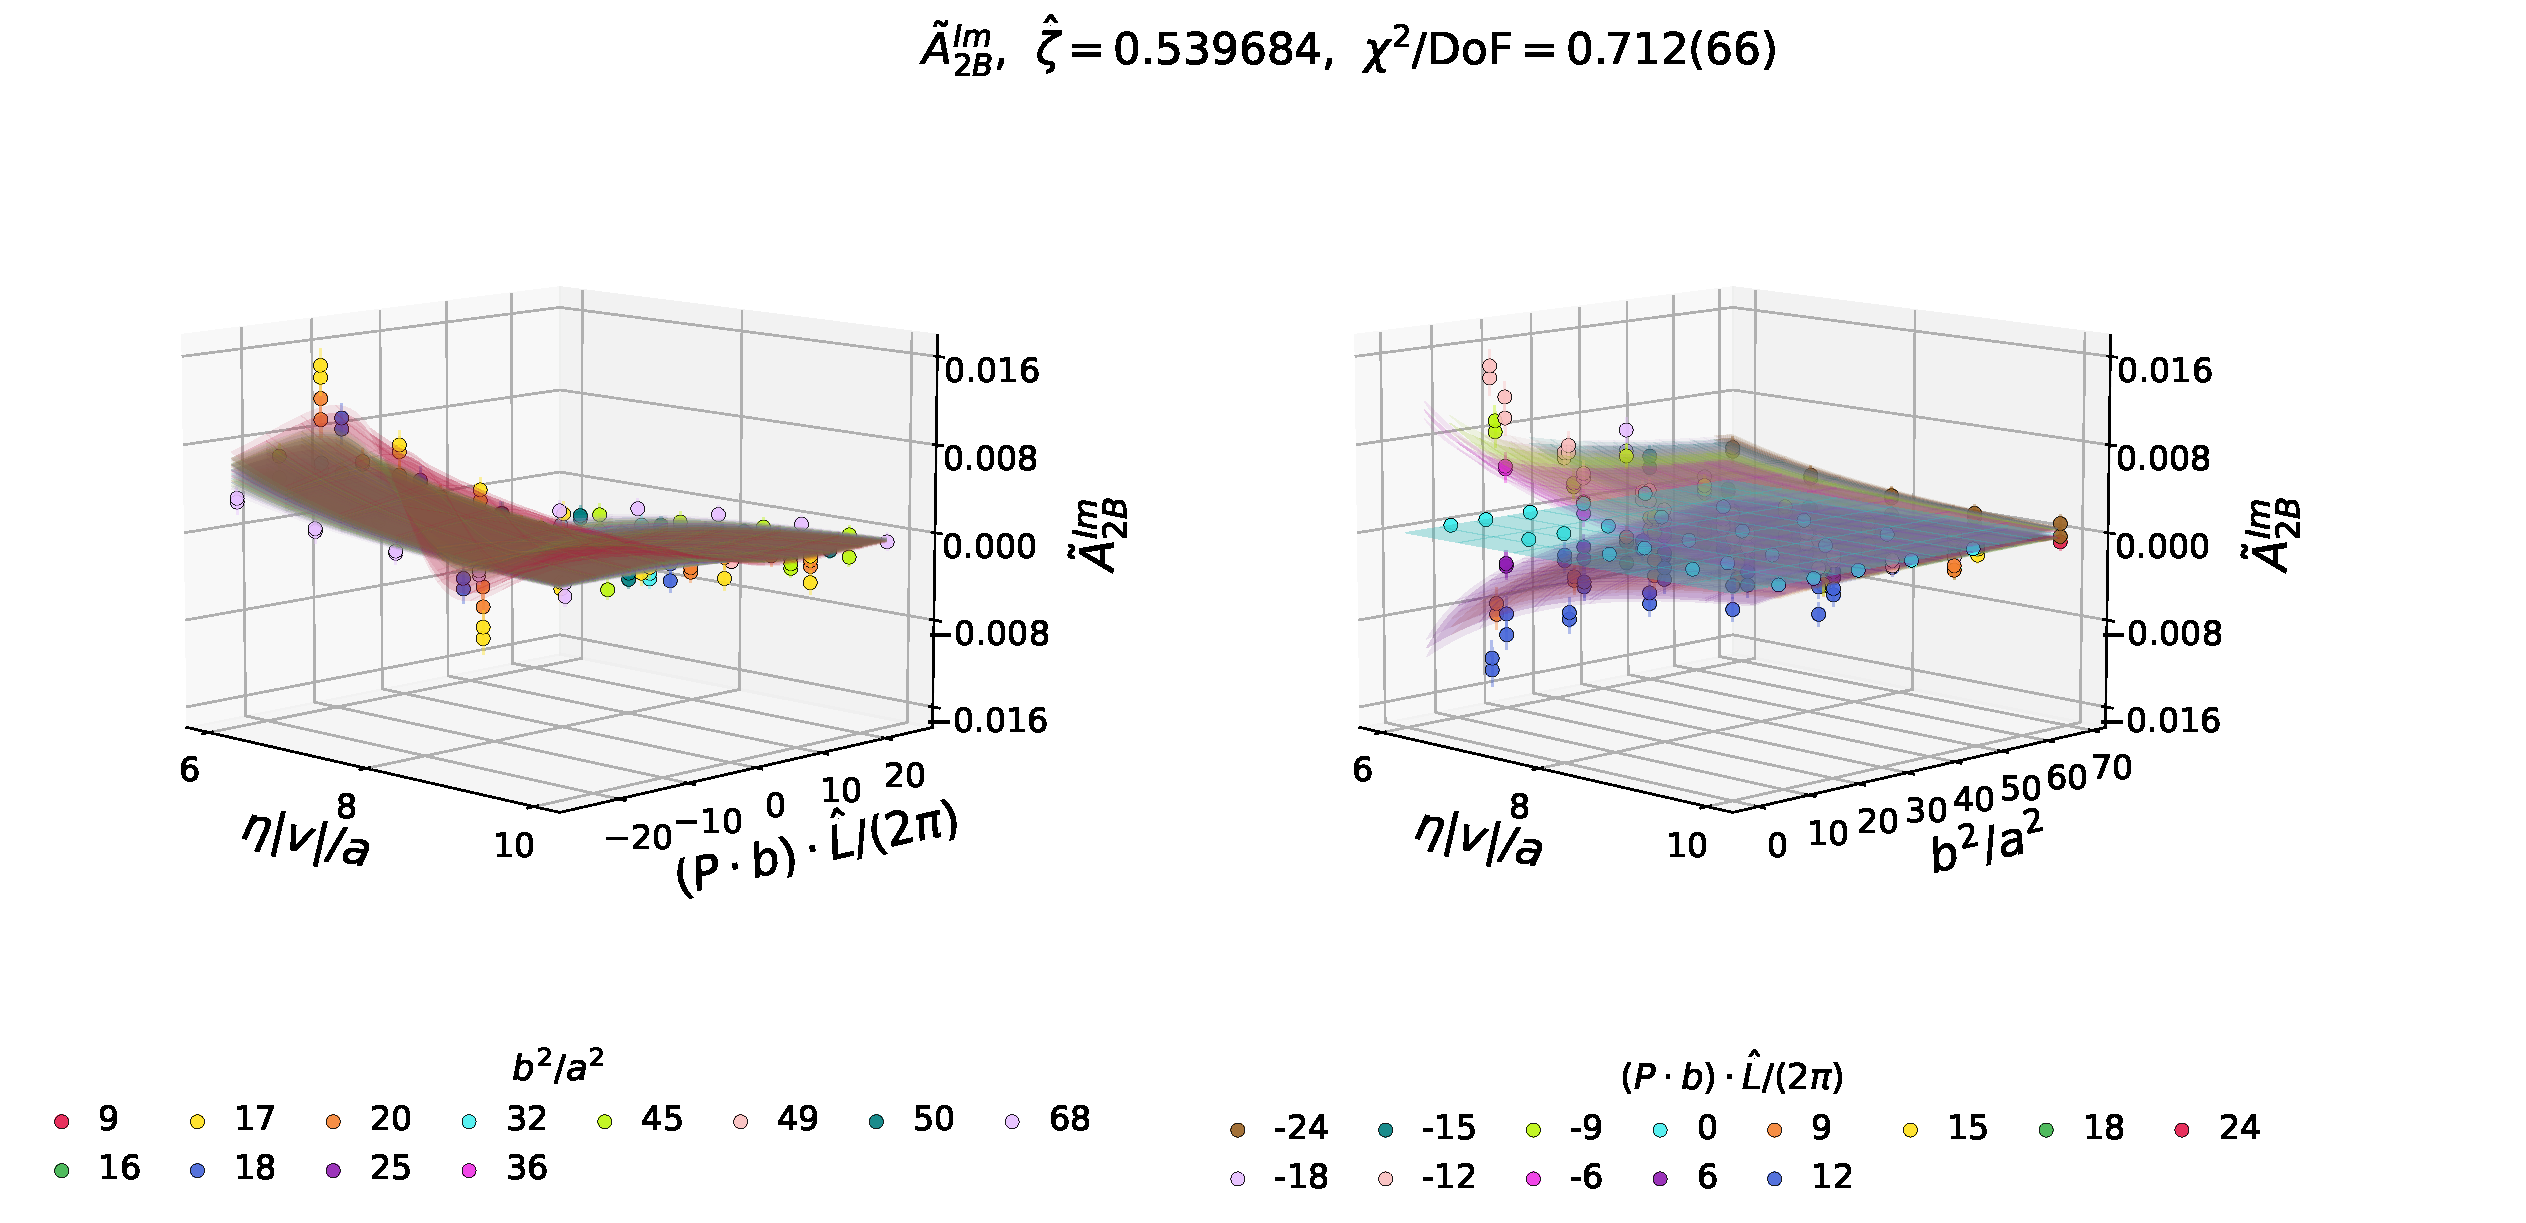
\includegraphics[width=\linewidth,height=.70\textheight,keepaspectratio]{fitting/ImA2B_Pb_bsq_PL-3_WithFit_3D.pdf}
\par\small Invariant coordinates: $(\nu,b^2,\eta)$. All panels and data overlays retained.

\figsrc{Thesis: plots; ImA2B\_Pb\_bsq\_PL-3\_WithFit\_3D}
\end{frame}

\begin{frame}{Fixed staple $\eta=8$: $\tAmp_{2B}^{\mathrm{Im}}$, $P_L=-3$}
\centering
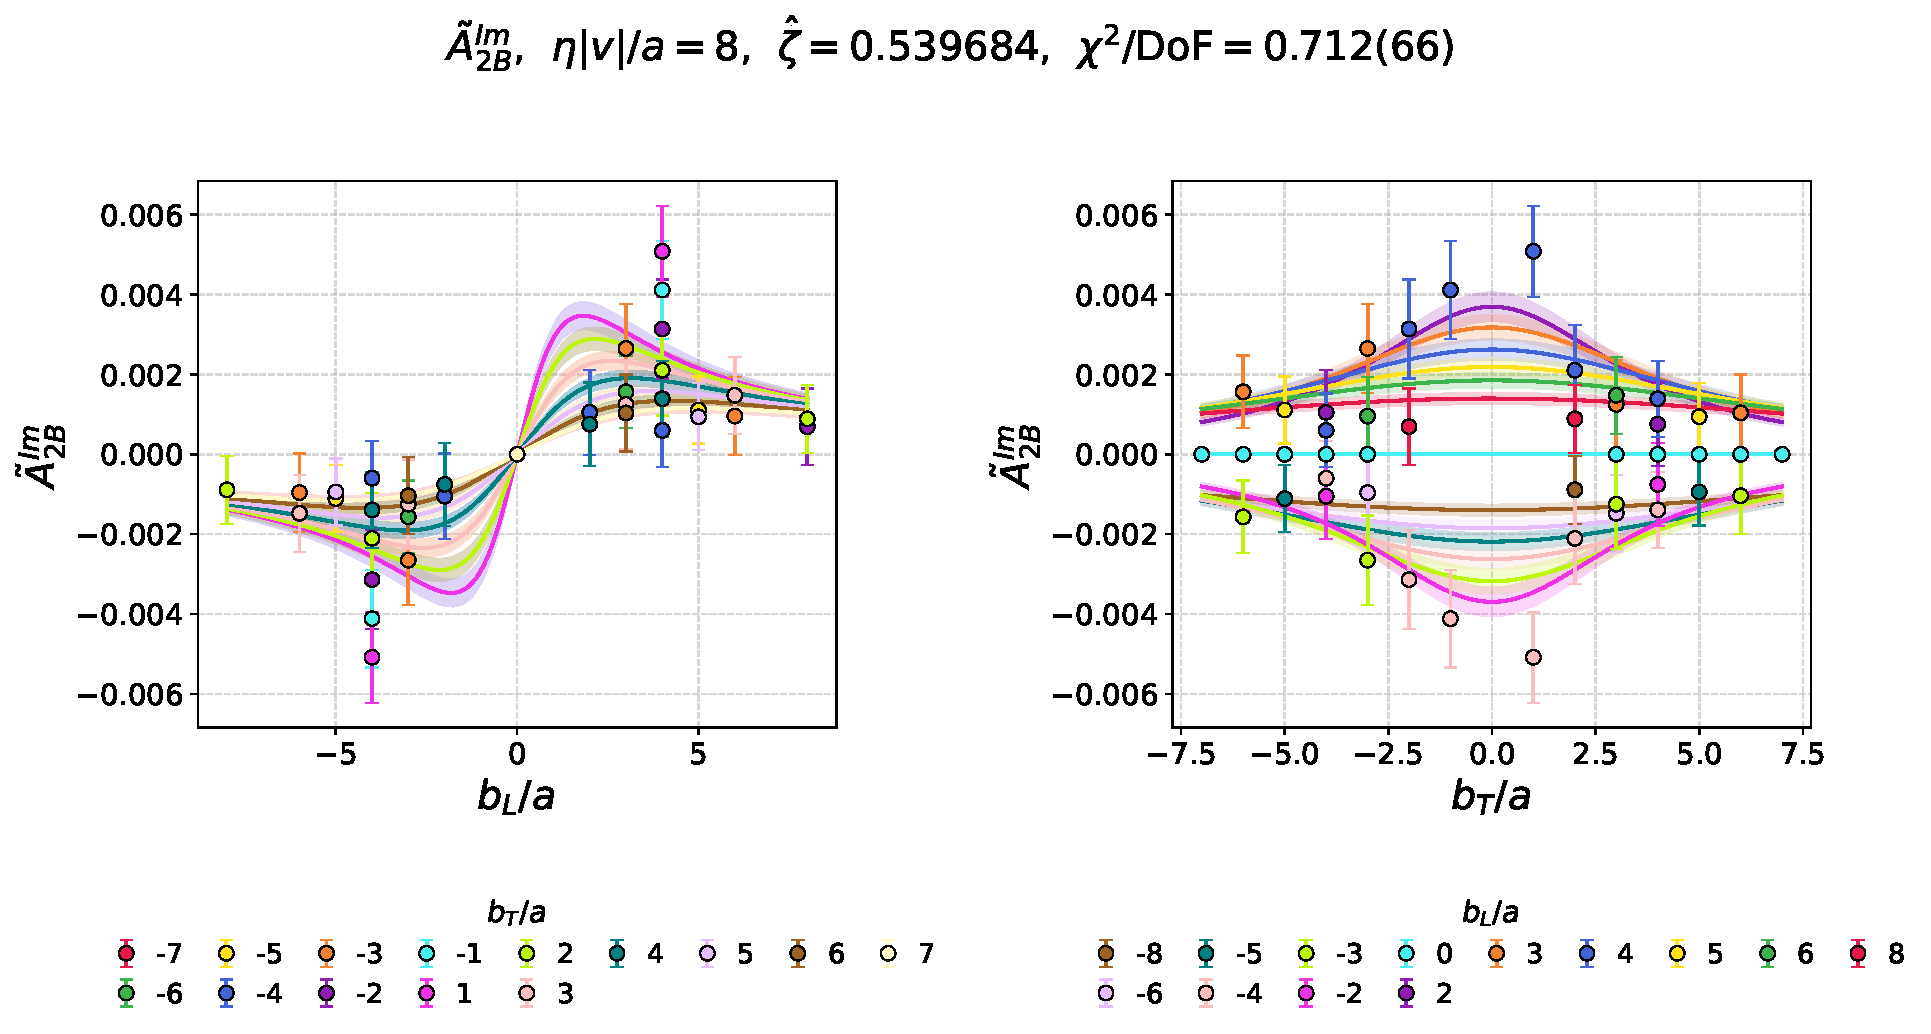
\includegraphics[width=\linewidth,height=.70\textheight,keepaspectratio]{fitting/ImA2B_eta8_PL-3_WithFit_2D.pdf}
\par\small Both spatial-coordinate slices. Same simultaneous fit, with Jackknife bands.

\figsrc{Thesis: plots; ImA2B\_eta8\_PL-3\_WithFit\_2D}
\end{frame}

\begin{frame}{Fixed staple $\eta=8$: $\tAmp_{2B}^{\mathrm{Im}}$, $P_L=-3$}
\centering
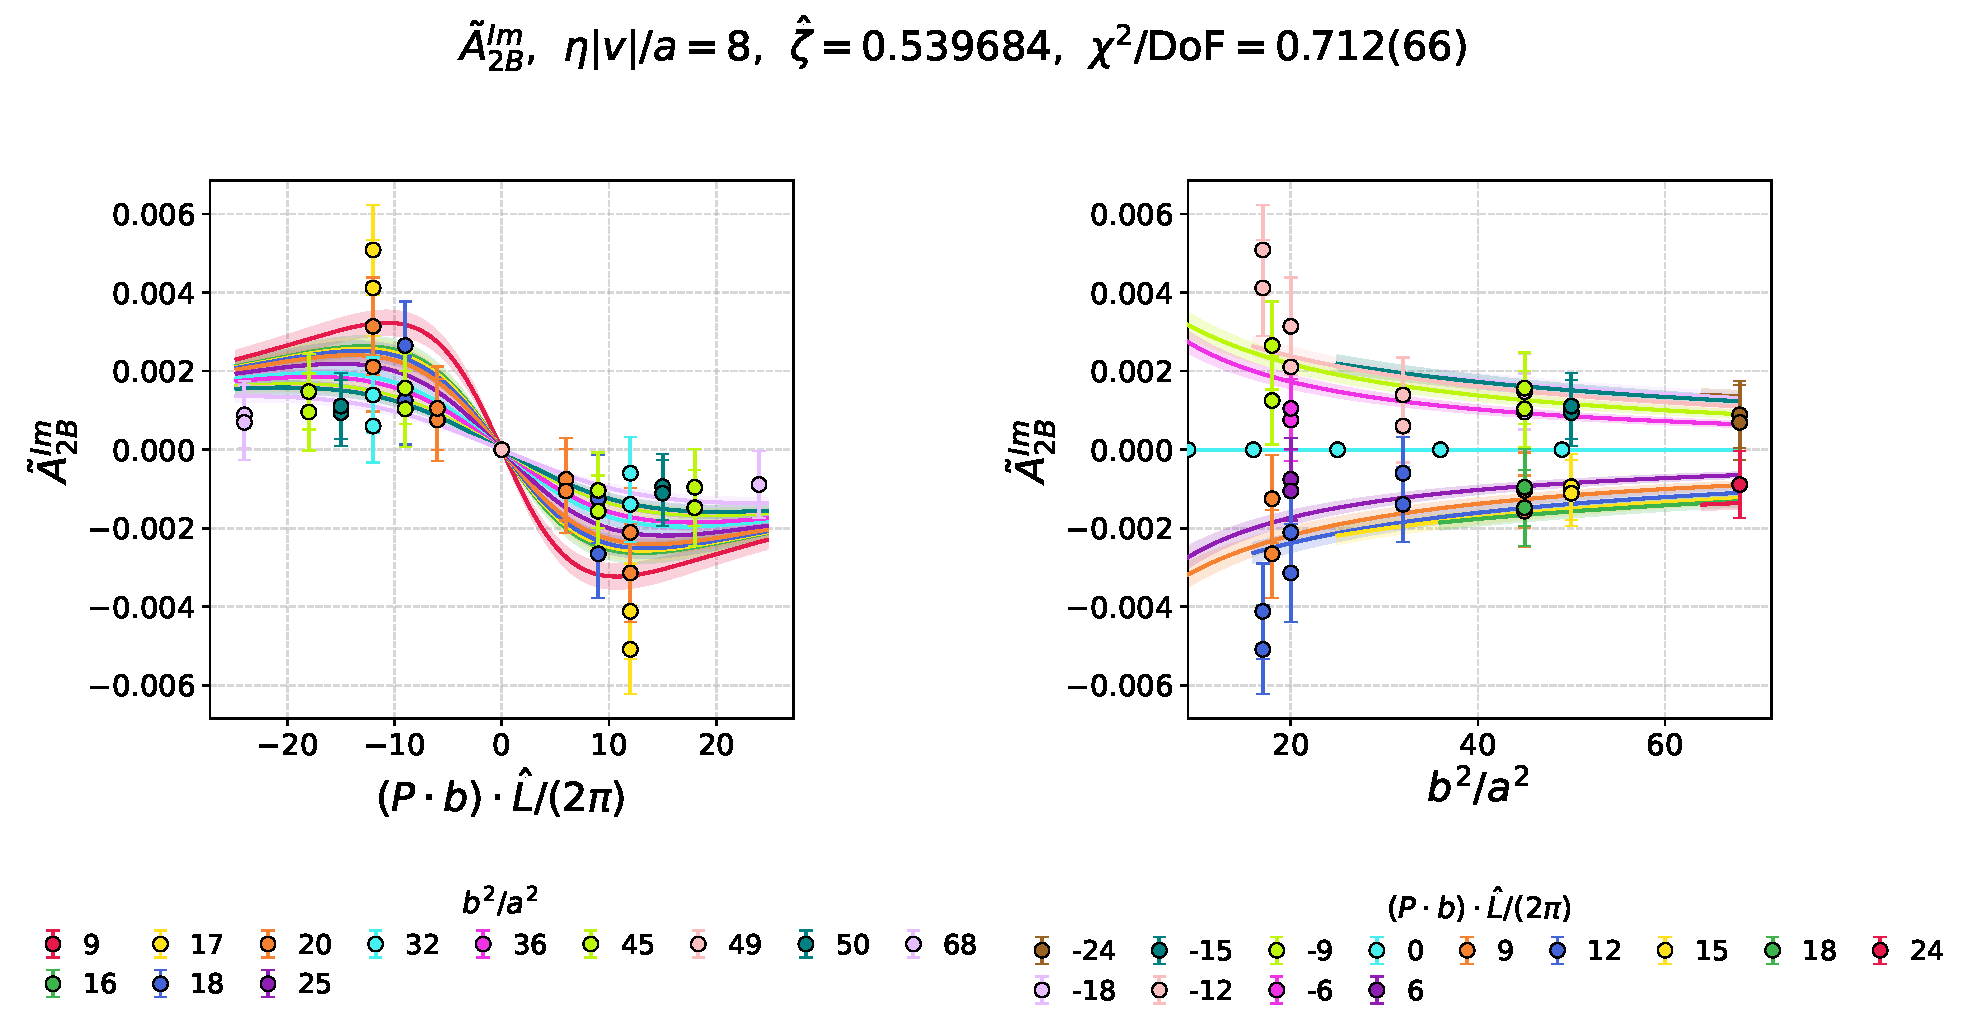
\includegraphics[width=\linewidth,height=.70\textheight,keepaspectratio]{fitting/ImA2B_Pb_bsq_eta8_PL-3_WithFit_2D.pdf}
\par\small Both invariant-coordinate slices. Same simultaneous fit, with Jackknife bands.

\figsrc{Thesis: plots; ImA2B\_Pb\_bsq\_eta8\_PL-3\_WithFit\_2D}
\end{frame}

\begin{frame}{Global fit: $\tAmp_{12B}^{\mathrm{Re}}$, $P_L=-3$}
\centering
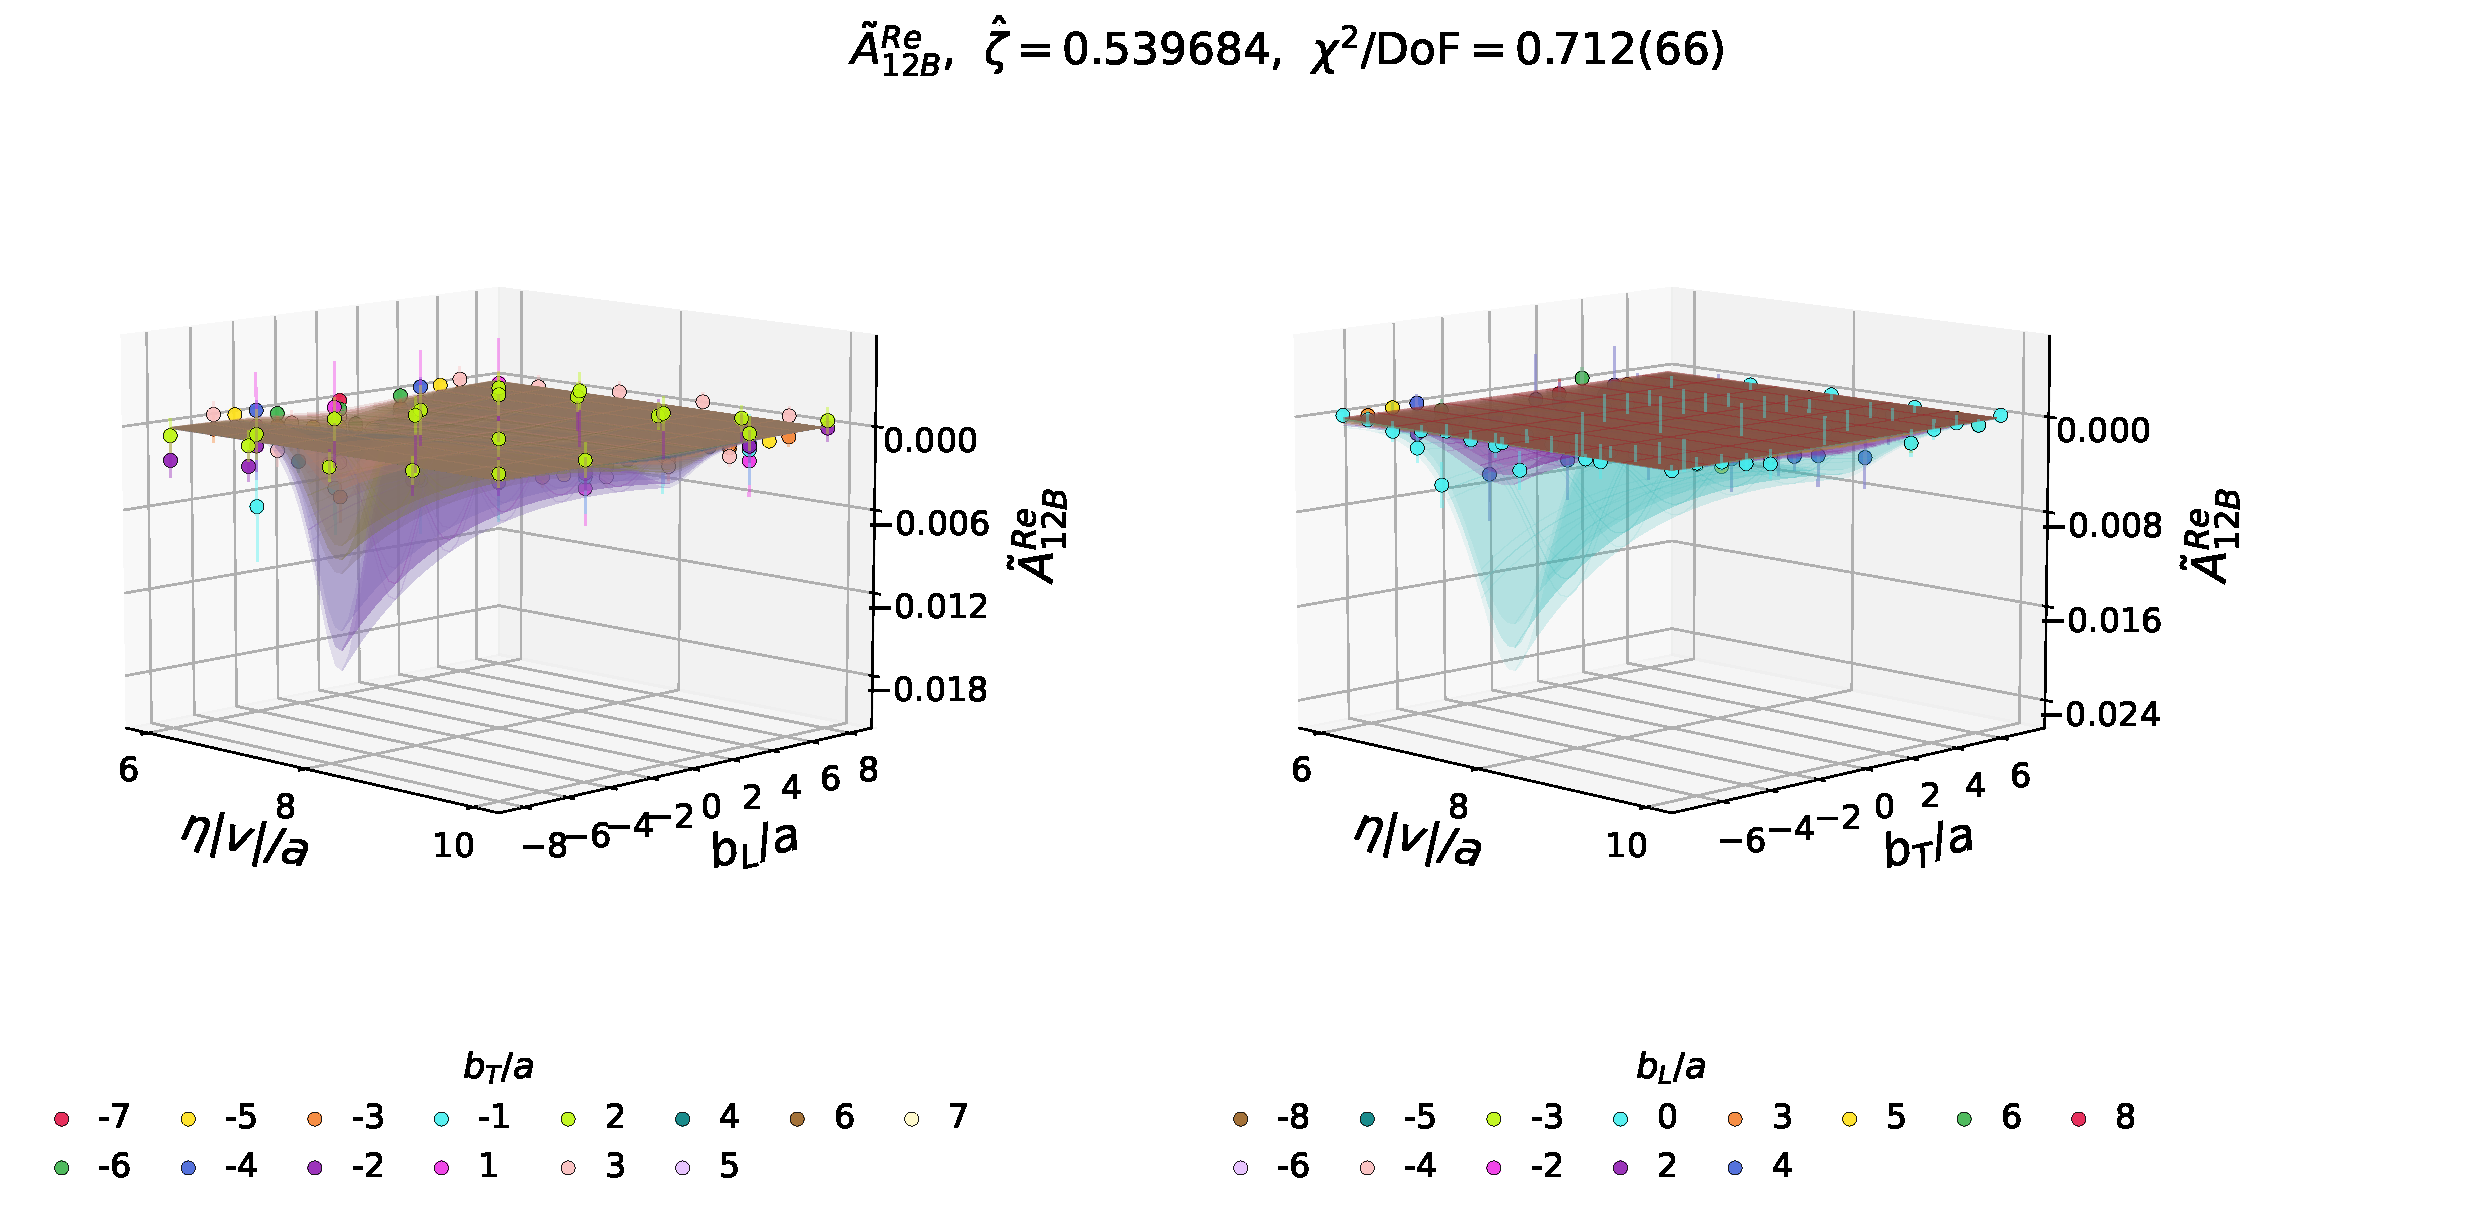
\includegraphics[width=\linewidth,height=.70\textheight,keepaspectratio]{fitting/ReA12B_PL-3_WithFit_3D.pdf}
\par\small Spatial coordinates: $(b_L,b_T,\eta)$. All panels and data overlays retained.

\figsrc{Thesis: plots; ReA12B\_PL-3\_WithFit\_3D}
\end{frame}

\begin{frame}{Global fit: $\tAmp_{12B}^{\mathrm{Re}}$, $P_L=-3$}
\centering
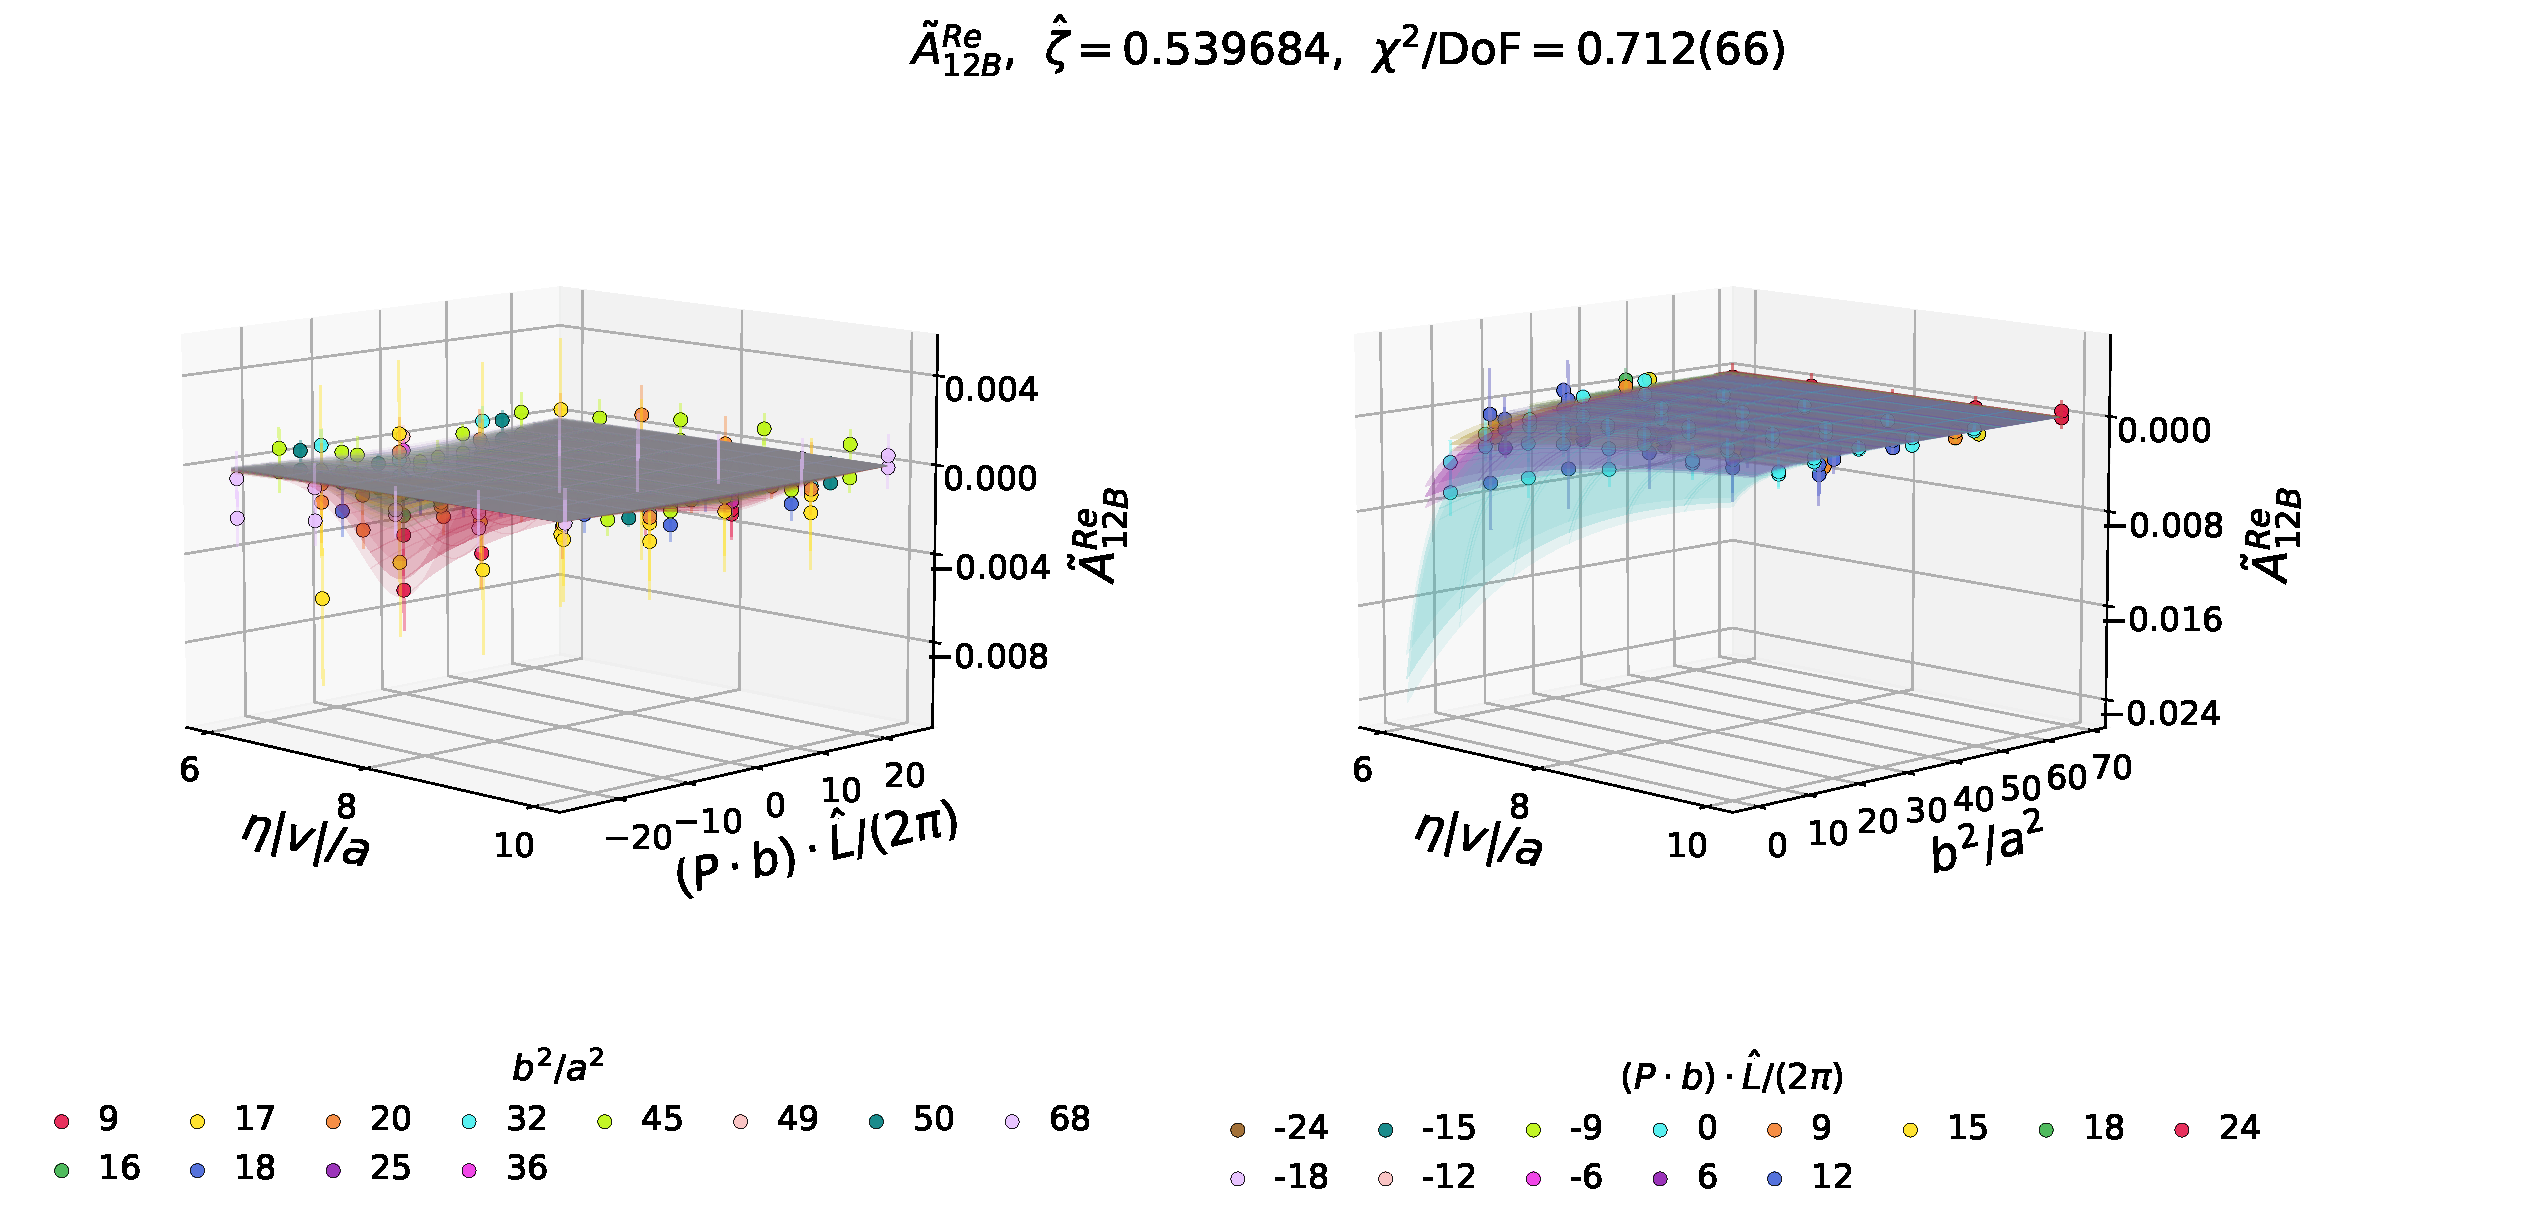
\includegraphics[width=\linewidth,height=.70\textheight,keepaspectratio]{fitting/ReA12B_Pb_bsq_PL-3_WithFit_3D.pdf}
\par\small Invariant coordinates: $(\nu,b^2,\eta)$. All panels and data overlays retained.

\figsrc{Thesis: plots; ReA12B\_Pb\_bsq\_PL-3\_WithFit\_3D}
\end{frame}

\begin{frame}{Fixed staple $\eta=8$: $\tAmp_{12B}^{\mathrm{Re}}$, $P_L=-3$}
\centering
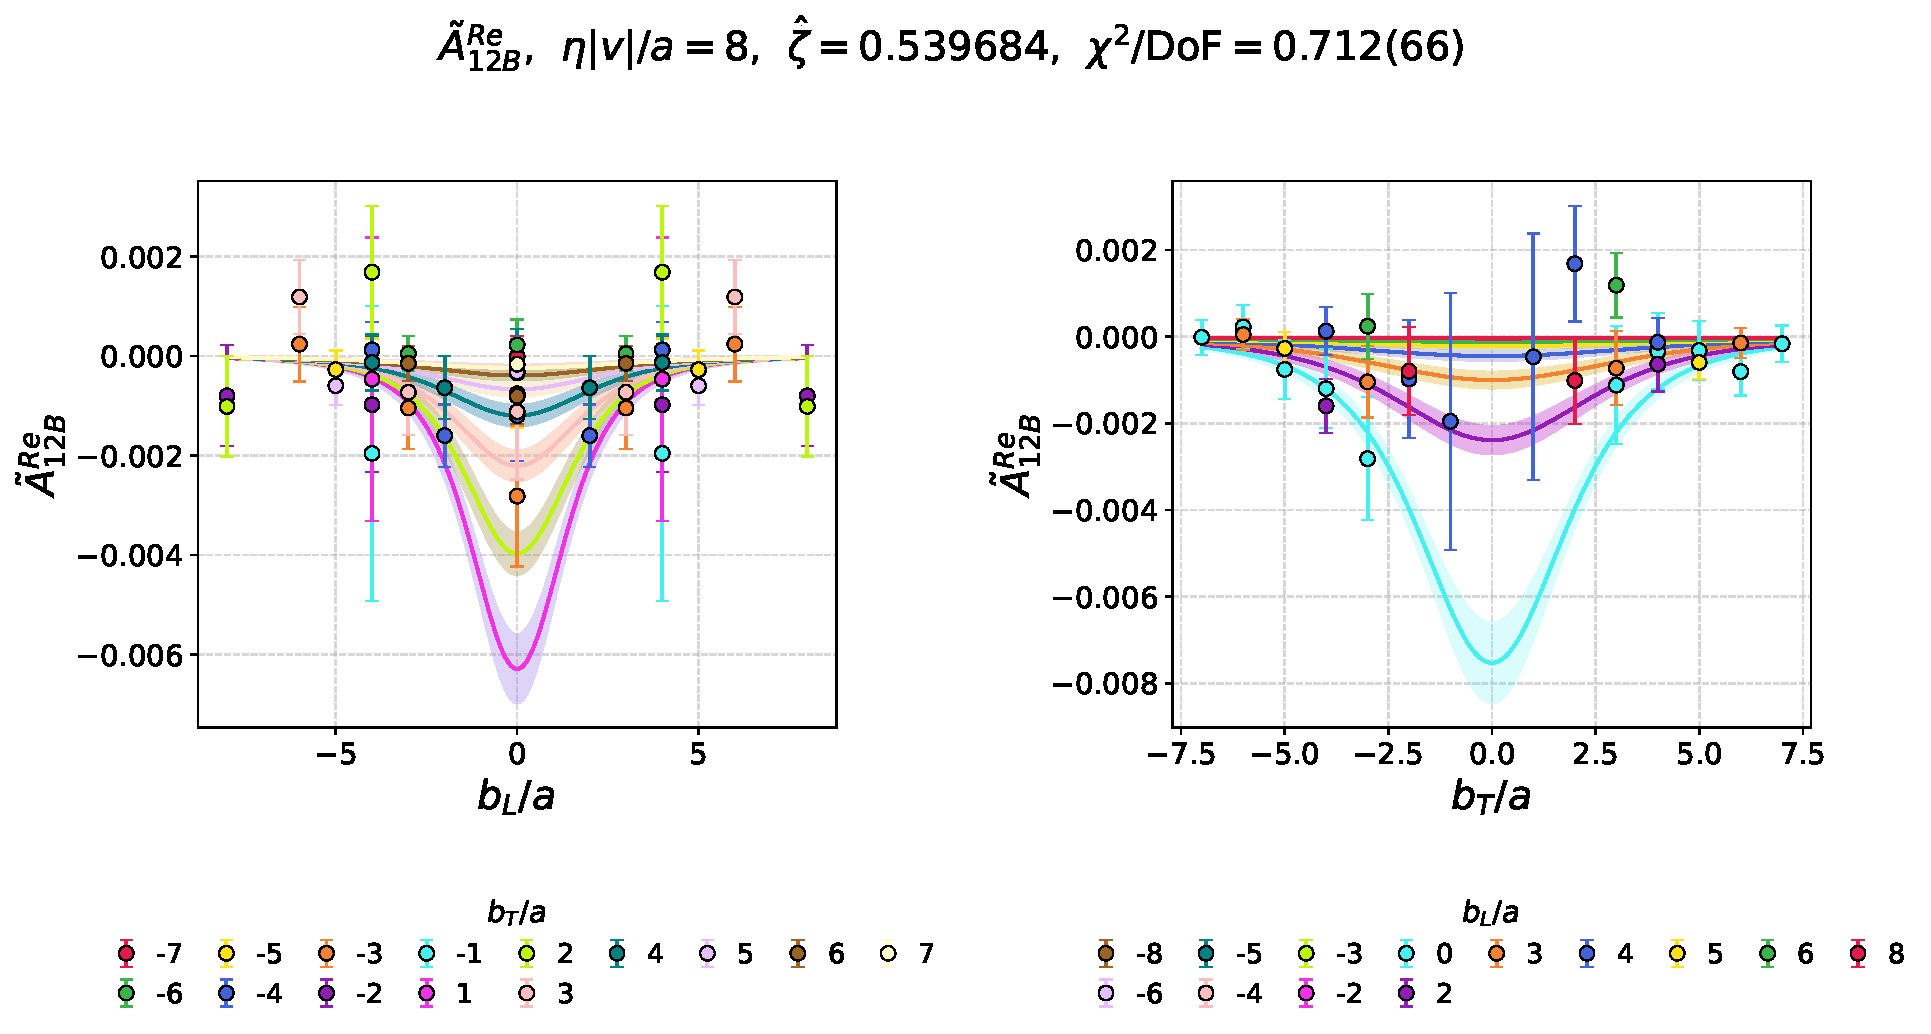
\includegraphics[width=\linewidth,height=.70\textheight,keepaspectratio]{fitting/ReA12B_eta8_PL-3_WithFit_2D.pdf}
\par\small Both spatial-coordinate slices. Same simultaneous fit, with Jackknife bands.

\figsrc{Thesis: plots; ReA12B\_eta8\_PL-3\_WithFit\_2D}
\end{frame}

\begin{frame}{Fixed staple $\eta=8$: $\tAmp_{12B}^{\mathrm{Re}}$, $P_L=-3$}
\centering
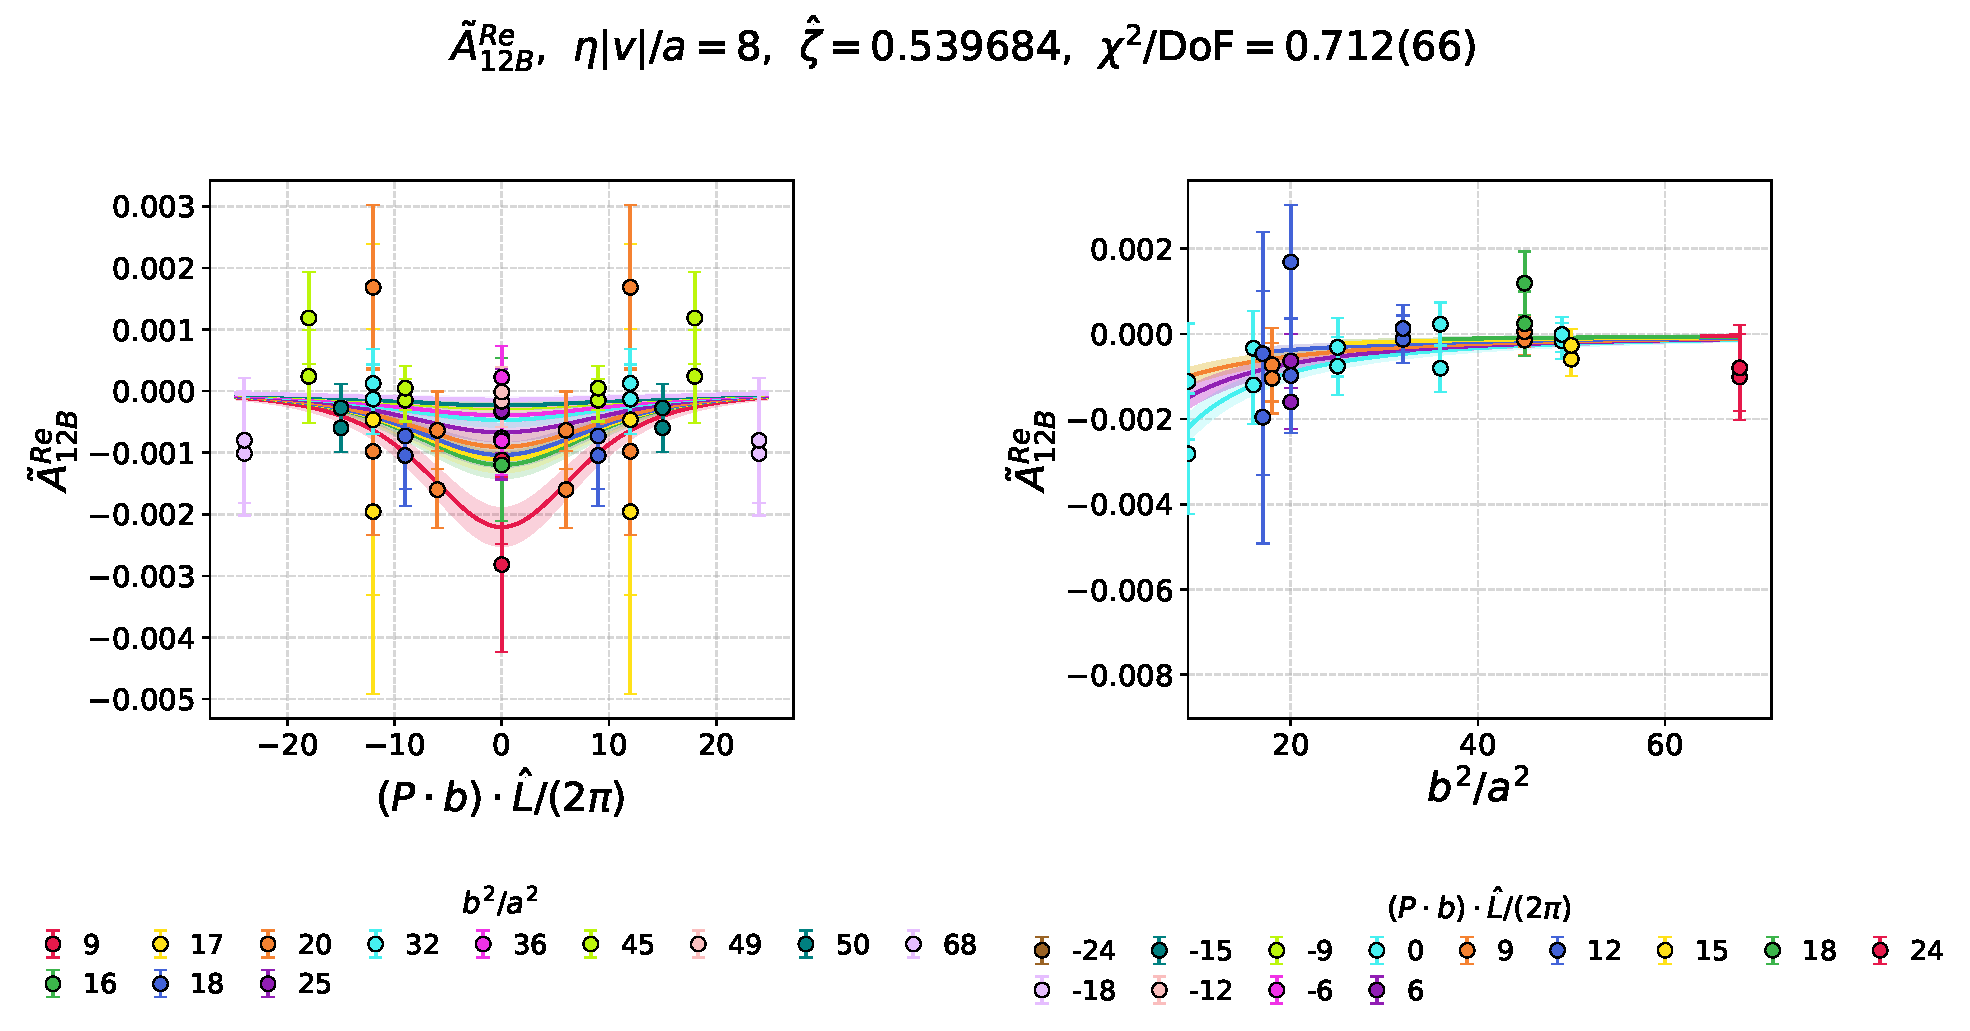
\includegraphics[width=\linewidth,height=.70\textheight,keepaspectratio]{fitting/ReA12B_Pb_bsq_eta8_PL-3_WithFit_2D.pdf}
\par\small Both invariant-coordinate slices. Same simultaneous fit, with Jackknife bands.

\figsrc{Thesis: plots; ReA12B\_Pb\_bsq\_eta8\_PL-3\_WithFit\_2D}
\end{frame}

\begin{frame}{Integrated Fourier results: $P_L=-3$}
\small\renewcommand{\arraystretch}{1.8}\begin{tabular}{lcccc}\toprule Integral & $(-\infty,\infty)$ & $[-1,1]$ & $[-1,0]$ & $[0,1]$\\\midrule
$\int dx\,E$ & 0.759(69) & 0.754(70) & 0.377(35) & 0.377(35) \\
$\int dx\,O$ & -1(320)e-17 & 2(33)e-16 & 0.234(23) & -0.235(23) \\
$\int dx\,\tilde f_1^{(0)}$ & 1.52(14) & 1.51(14) & 0.286(55) & 1.22(11) \\
$\int dx\,\tilde f_{1T}^{\perp(1)}$ & 0.333(51) & 0.333(51) & 0.167(25) & 0.167(25) \\
$m_N\int dx\,\tilde f_{1T}^{\perp(1)}/\int dx\,\tilde f_1^{(0)}$ & 0.236(32) & 0.238(32) & 0.63(13) & 0.147(20) \\
\bottomrule\end{tabular}\par\medskip $b^2=9a^2$; all values and Jackknife uncertainties retained. Numerical values retain the source normalization. The last row is in GeV.
\figsrc{Thesis: SimultaneousFitsCov/Integration\_Table\_PL-3\_bmin3\_b2-9.tex}
\end{frame}

\begin{frame}{Fourier results (2D): $P_L=-3$, unpolarized}
\centering
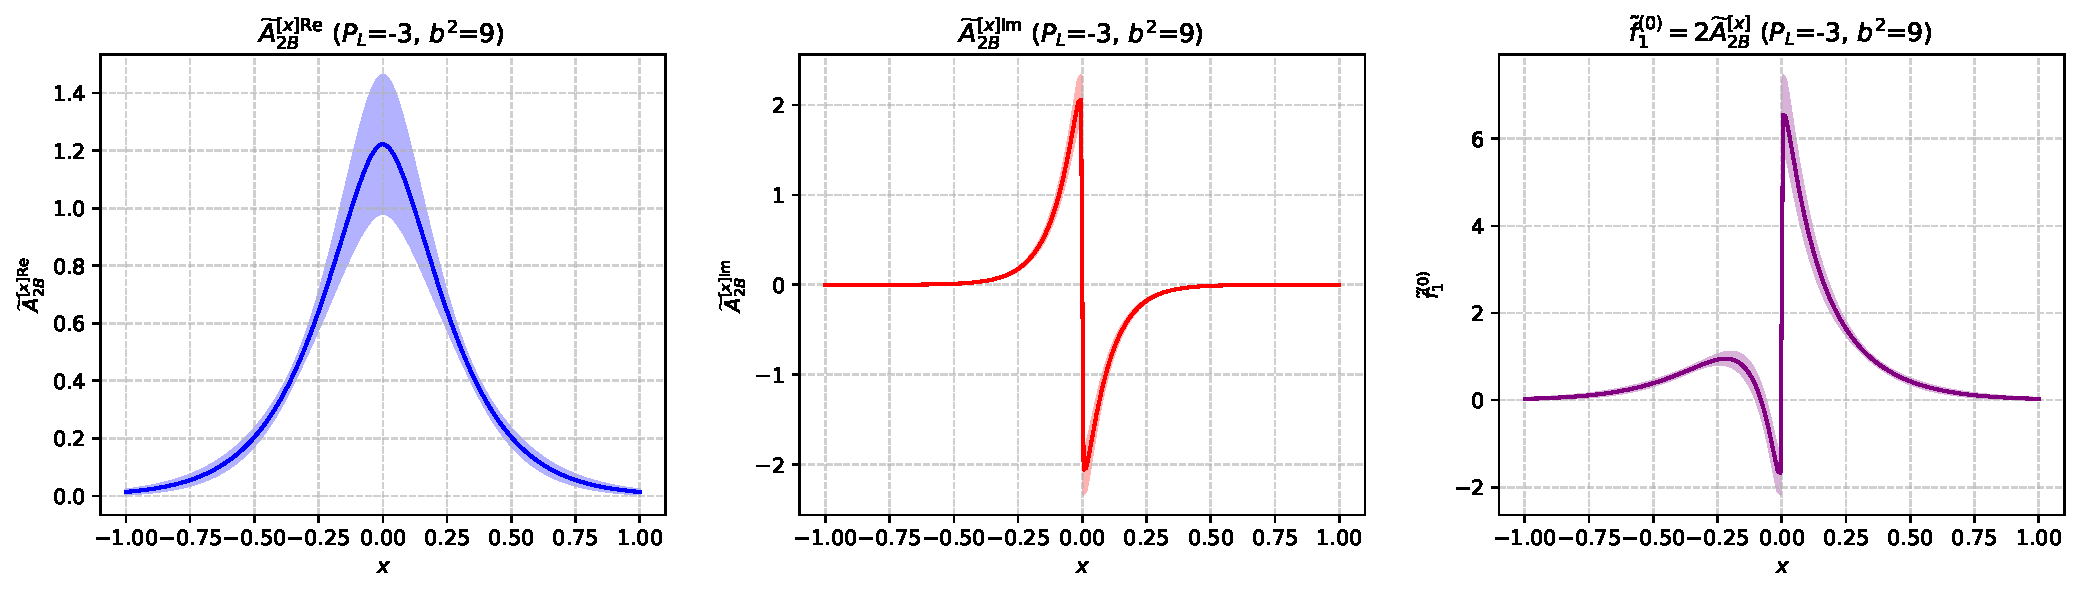
\includegraphics[width=\linewidth,height=.70\textheight,keepaspectratio]{fitting/FT_xdep_A2B_A12B_bmin3_eta610_b2-9_PL-3__row1.pdf}
\par\small Even, odd, and unpolarized transforms. Fixed $b^2=9a^2$.

\figsrc{Thesis: SimultaneousFitsCov; FT\_xdep\_A2B\_A12B\_bmin3\_eta610\_b2-9\_PL-3}
\end{frame}

\begin{frame}{Fourier results (2D): $P_L=-3$, Sivers}
\centering
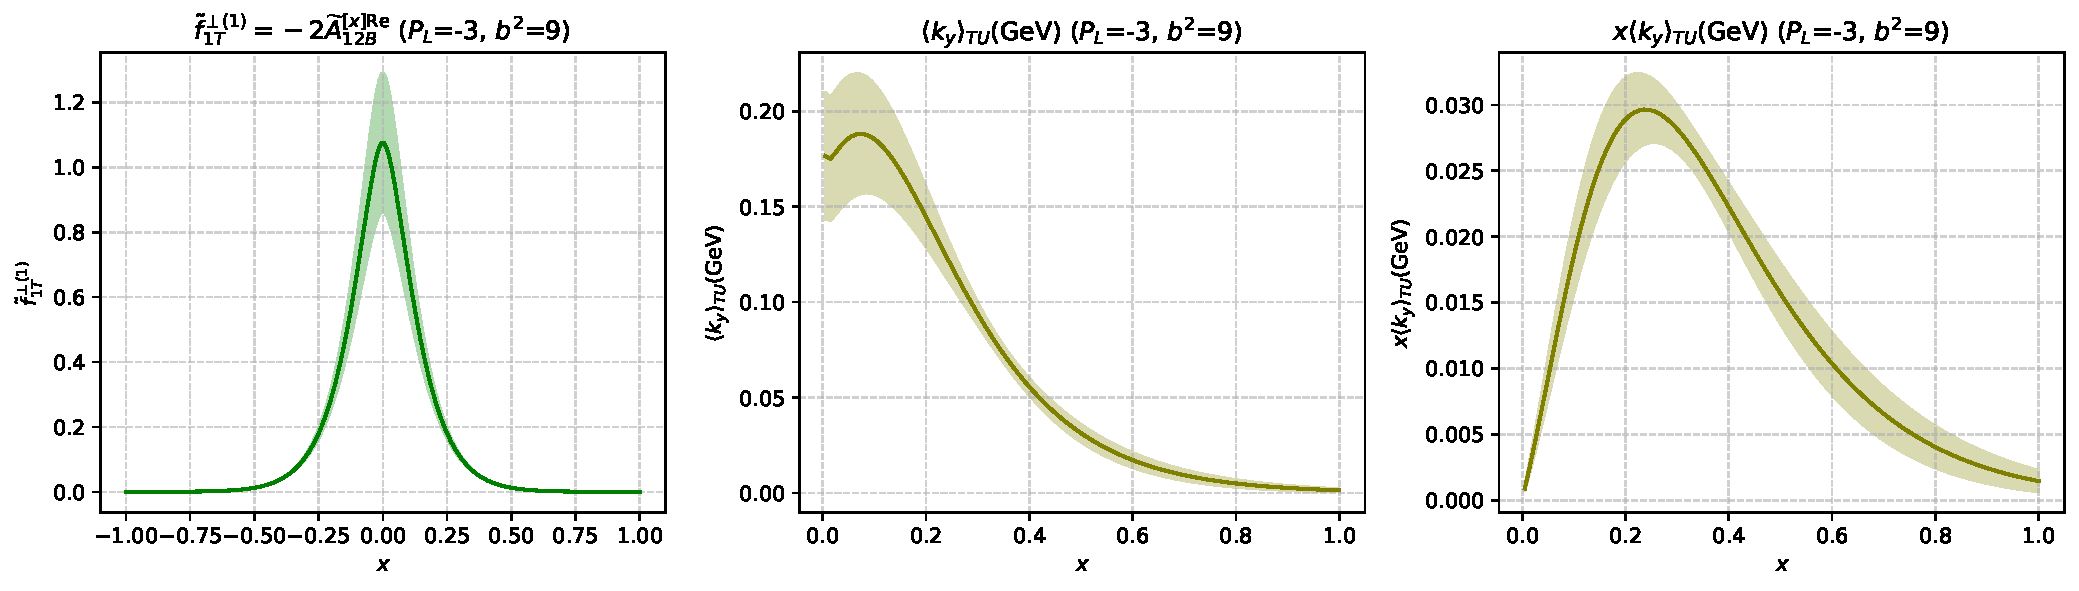
\includegraphics[width=\linewidth,height=.70\textheight,keepaspectratio]{fitting/FT_xdep_A2B_A12B_bmin3_eta610_b2-9_PL-3__row2.pdf}
\par\small Sivers transform, shift, and $x\langle k_y\rangle_{TU}$. Fixed $b^2=9a^2$.

\figsrc{Thesis: SimultaneousFitsCov; FT\_xdep\_A2B\_A12B\_bmin3\_eta610\_b2-9\_PL-3}
\end{frame}

\begin{frame}{Fourier results (3D): $P_L=-3$, unpolarized}
\centering
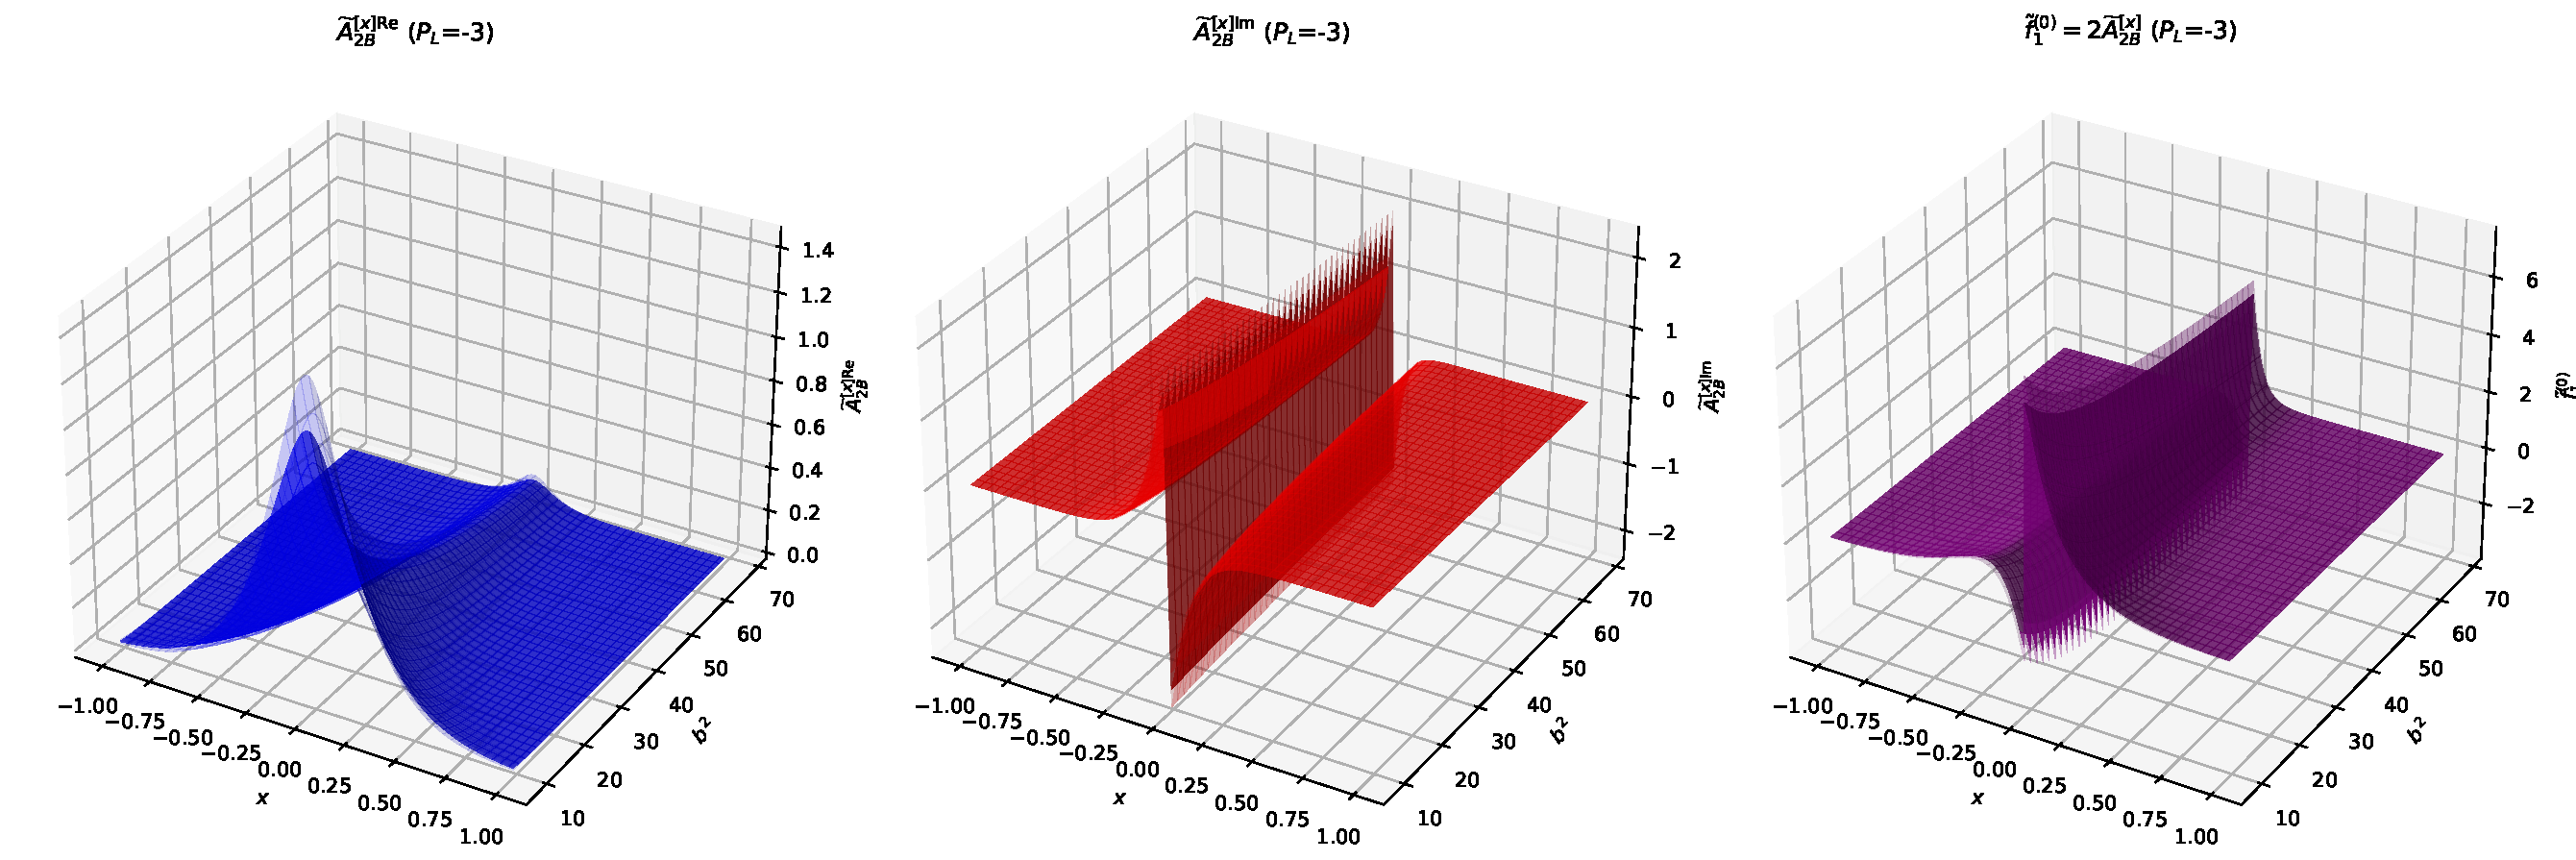
\includegraphics[width=\linewidth,height=.70\textheight,keepaspectratio]{fitting/FT_xdep_3D_A2B_A12B_bmin3_eta610_PL-3__row1.pdf}
\par\small Even, odd, and unpolarized transforms. Full $b^2/a^2\in[9,68]$ dependence.

\figsrc{Thesis: SimultaneousFitsCov; FT\_xdep\_3D\_A2B\_A12B\_bmin3\_eta610\_PL-3}
\end{frame}

\begin{frame}{Fourier results (3D): $P_L=-3$, Sivers}
\centering
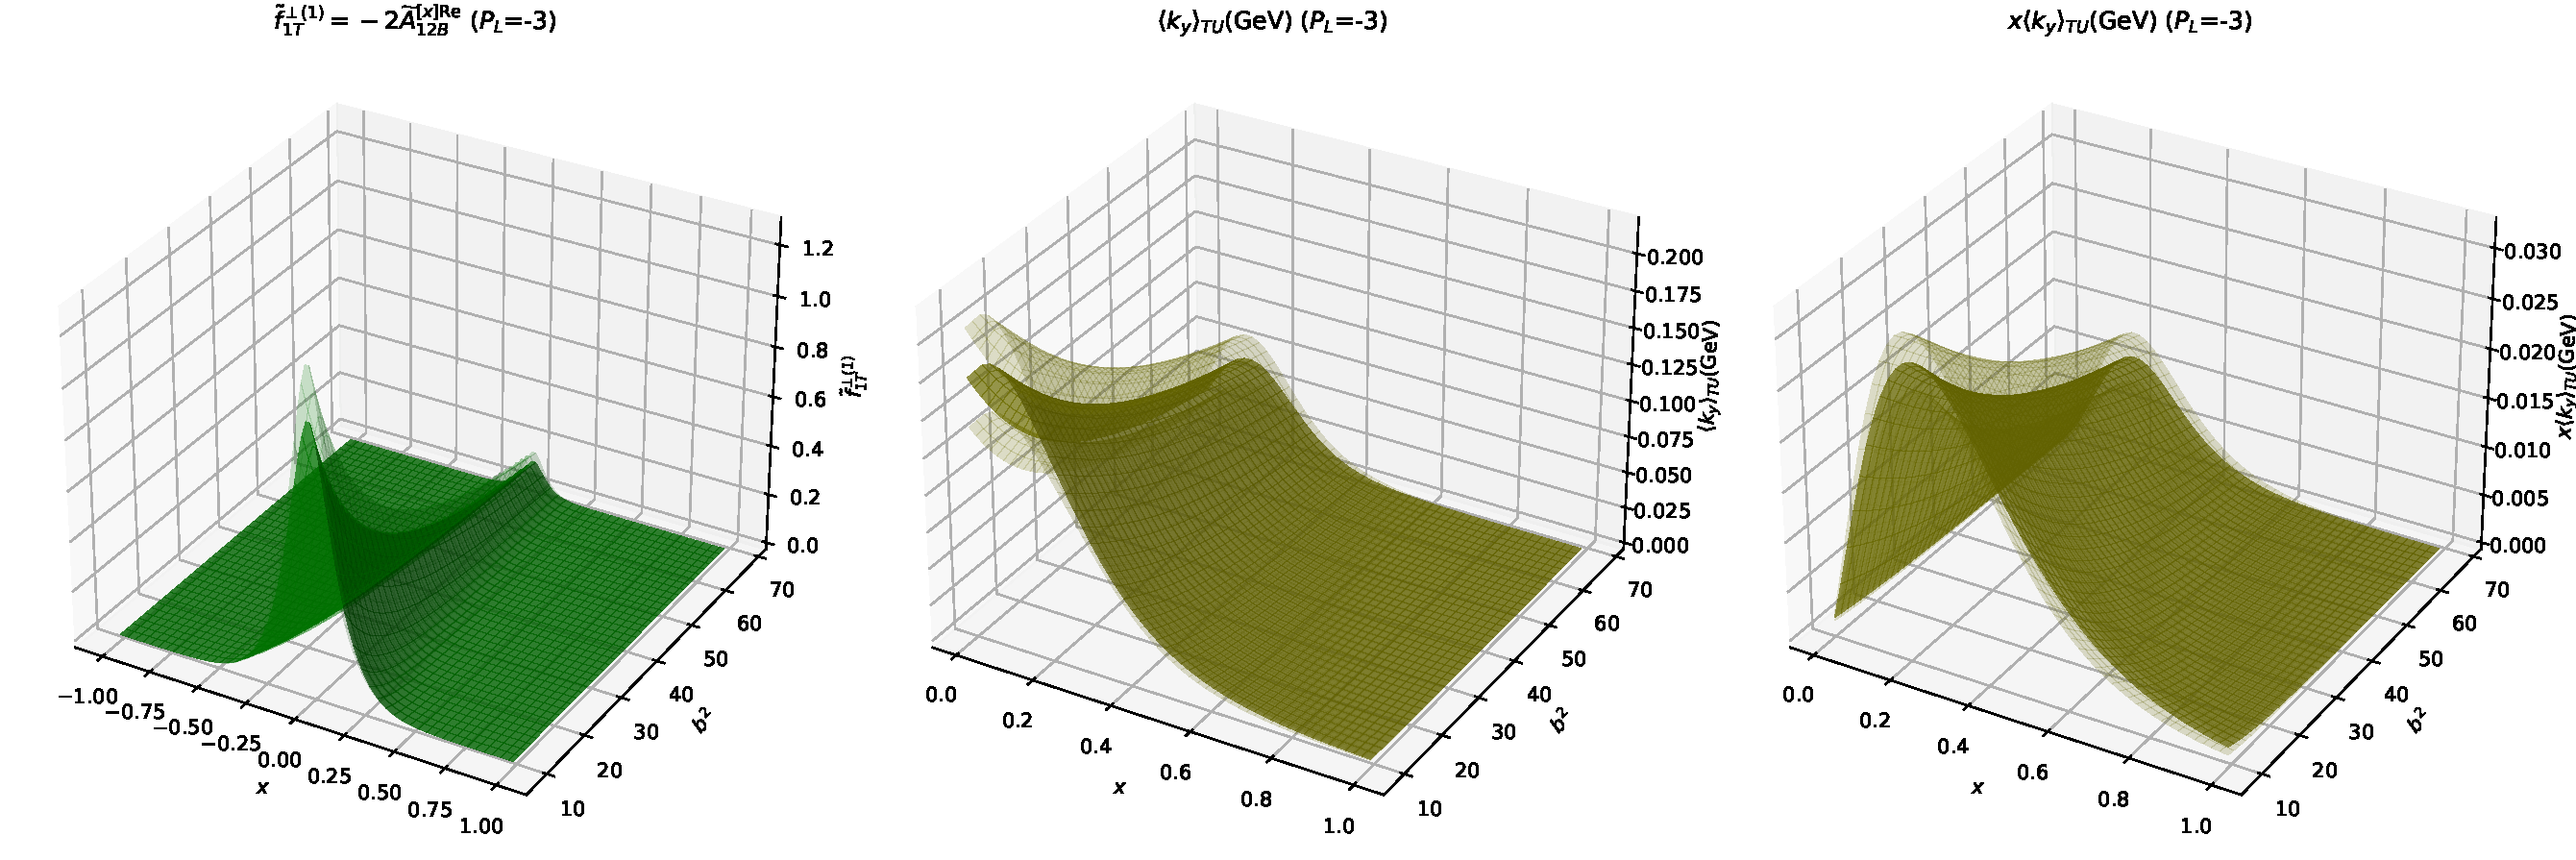
\includegraphics[width=\linewidth,height=.70\textheight,keepaspectratio]{fitting/FT_xdep_3D_A2B_A12B_bmin3_eta610_PL-3__row2.pdf}
\par\small Sivers transform, shift, and $x\langle k_y\rangle_{TU}$. Full $b^2/a^2\in[9,68]$ dependence.

\figsrc{Thesis: SimultaneousFitsCov; FT\_xdep\_3D\_A2B\_A12B\_bmin3\_eta610\_PL-3}
\end{frame}

\begin{frame}{Simultaneous fit parameters: $P_L=-4$}
\small $|\vect b|\ge3a$, $6\le\eta\le10$; reported $\chi^2_{\rm aug}/N_{\rm data}=0.434(51)$.\par\medskip
\begin{columns}[t]\begin{column}{.32\textwidth}\centering $\tAmp_{2B}^{\mathrm{Re}}$\par\medskip\renewcommand{\arraystretch}{1.3}\begin{tabular}{cc}\toprule Parameter & Value\\\midrule
$a$ & $4.0086(15)$ \\
$c$ & $0.27(21)$ \\
$d$ & $0.122(13)$ \\
$k_1$ & $12.2751(58)$ \\
$k_2$ & $-36.19925(89)$ \\
$j$ & $2.0654(56)$ \\
$f$ & $0.577(19)$ \\\bottomrule\end{tabular}\end{column}\begin{column}{.32\textwidth}\centering $\tAmp_{2B}^{\mathrm{Im}}$\par\medskip\renewcommand{\arraystretch}{1.3}\begin{tabular}{cc}\toprule Parameter & Value\\\midrule
$a''$ & $0.269(13)$ \\
$c''$ & $0.264(47)$ \\
$d''$ & $0.196(14)$ \\
$j''$ & $1.0084(79)$ \\
$f$ & $0.577(19)$ \\\bottomrule\end{tabular}\end{column}\begin{column}{.32\textwidth}\centering $\tAmp_{12B}^{\mathrm{Re}}$\par\medskip\renewcommand{\arraystretch}{1.3}\begin{tabular}{cc}\toprule Parameter & Value\\\midrule
$a'$ & $0.5824(55)$ \\
$c'$ & $0.116(19)$ \\
$d'$ & $0.102(18)$ \\
$j'$ & $2.0059(34)$ \\
$f$ & $0.577(19)$ \\\bottomrule\end{tabular}\end{column}\end{columns}
\figsrc{Thesis: SimultaneousFitsCov/Fit\_Table\_PL-4\_bmin3.tex}
\end{frame}

\begin{frame}{Global fit: $\tAmp_{2B}^{\mathrm{Re}}$, $P_L=-4$}
\centering
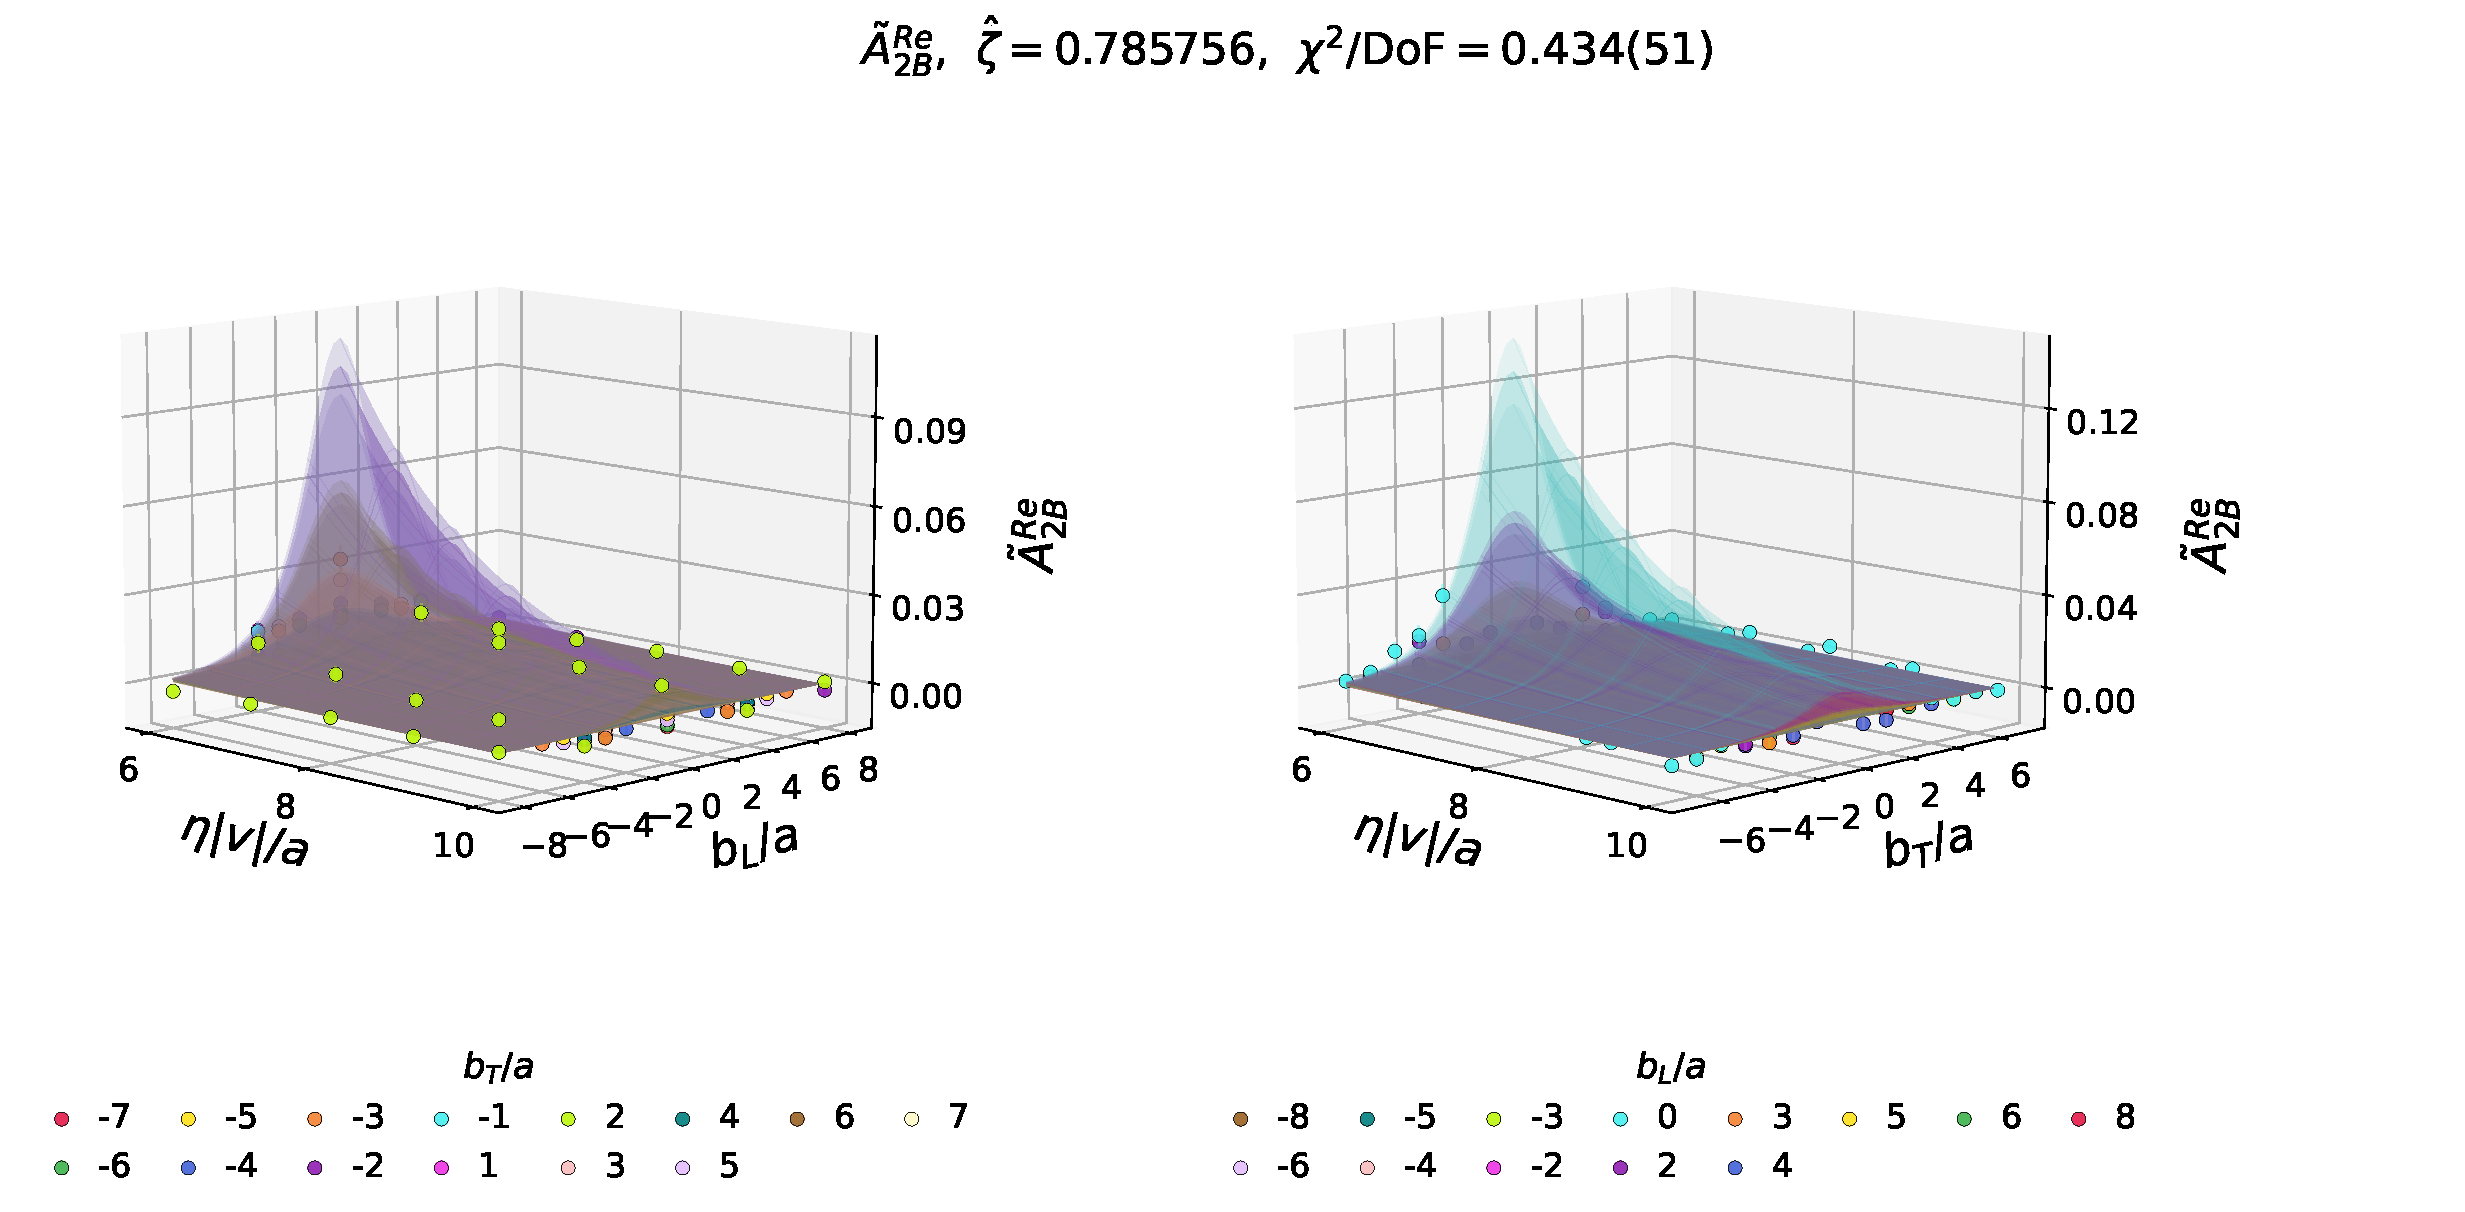
\includegraphics[width=\linewidth,height=.70\textheight,keepaspectratio]{fitting/ReA2B_PL-4_WithFit_3D.pdf}
\par\small Spatial coordinates: $(b_L,b_T,\eta)$. All panels and data overlays retained.

\figsrc{Thesis: plots; ReA2B\_PL-4\_WithFit\_3D}
\end{frame}

\begin{frame}{Global fit: $\tAmp_{2B}^{\mathrm{Re}}$, $P_L=-4$}
\centering
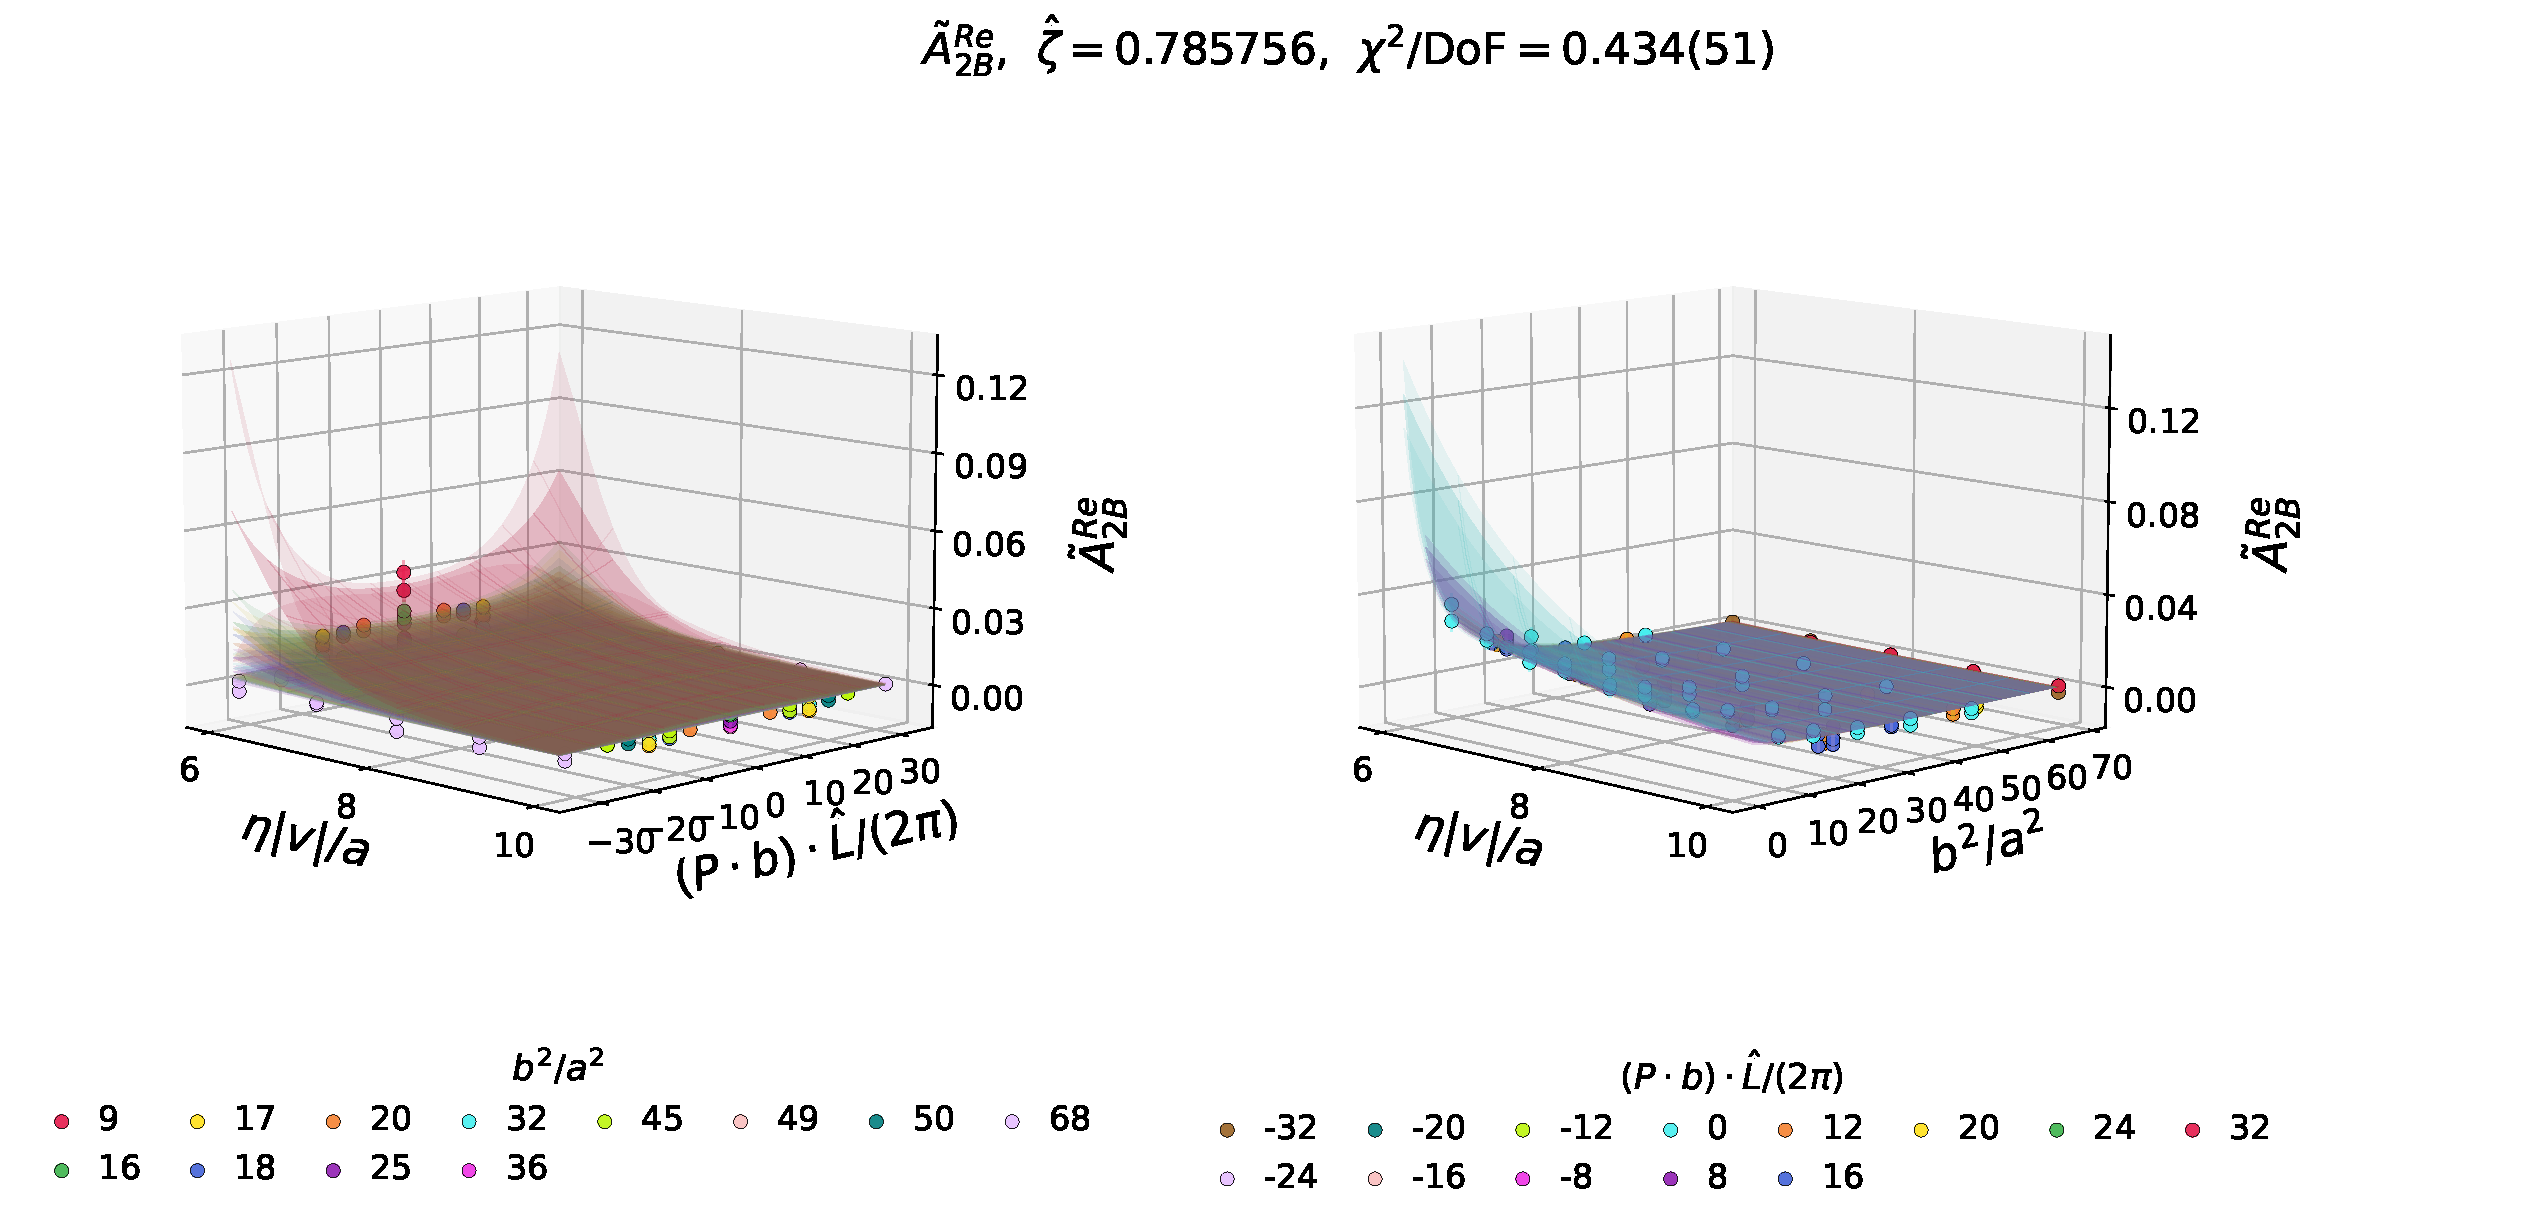
\includegraphics[width=\linewidth,height=.70\textheight,keepaspectratio]{fitting/ReA2B_Pb_bsq_PL-4_WithFit_3D.pdf}
\par\small Invariant coordinates: $(\nu,b^2,\eta)$. All panels and data overlays retained.

\figsrc{Thesis: plots; ReA2B\_Pb\_bsq\_PL-4\_WithFit\_3D}
\end{frame}

\begin{frame}{Fixed staple $\eta=8$: $\tAmp_{2B}^{\mathrm{Re}}$, $P_L=-4$}
\centering
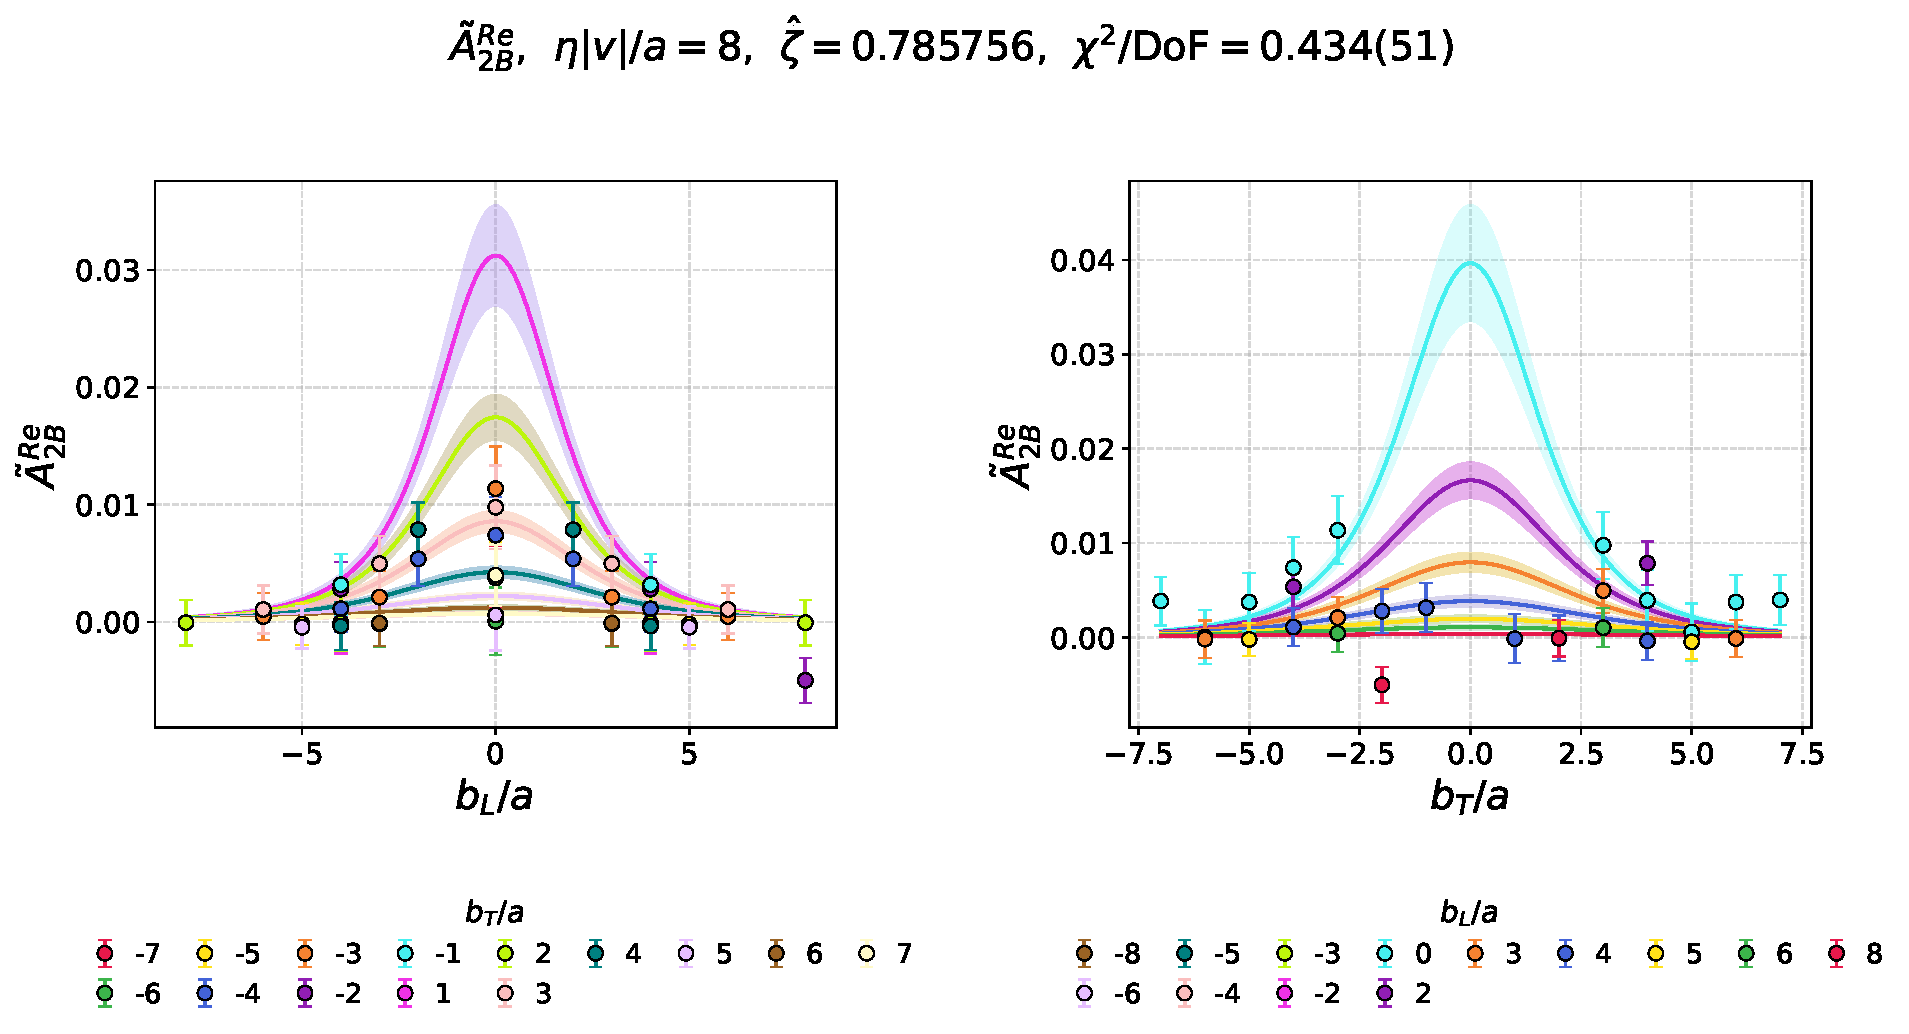
\includegraphics[width=\linewidth,height=.70\textheight,keepaspectratio]{fitting/ReA2B_eta8_PL-4_WithFit_2D.pdf}
\par\small Both spatial-coordinate slices. Same simultaneous fit, with Jackknife bands.

\figsrc{Thesis: plots; ReA2B\_eta8\_PL-4\_WithFit\_2D}
\end{frame}

\begin{frame}{Fixed staple $\eta=8$: $\tAmp_{2B}^{\mathrm{Re}}$, $P_L=-4$}
\centering
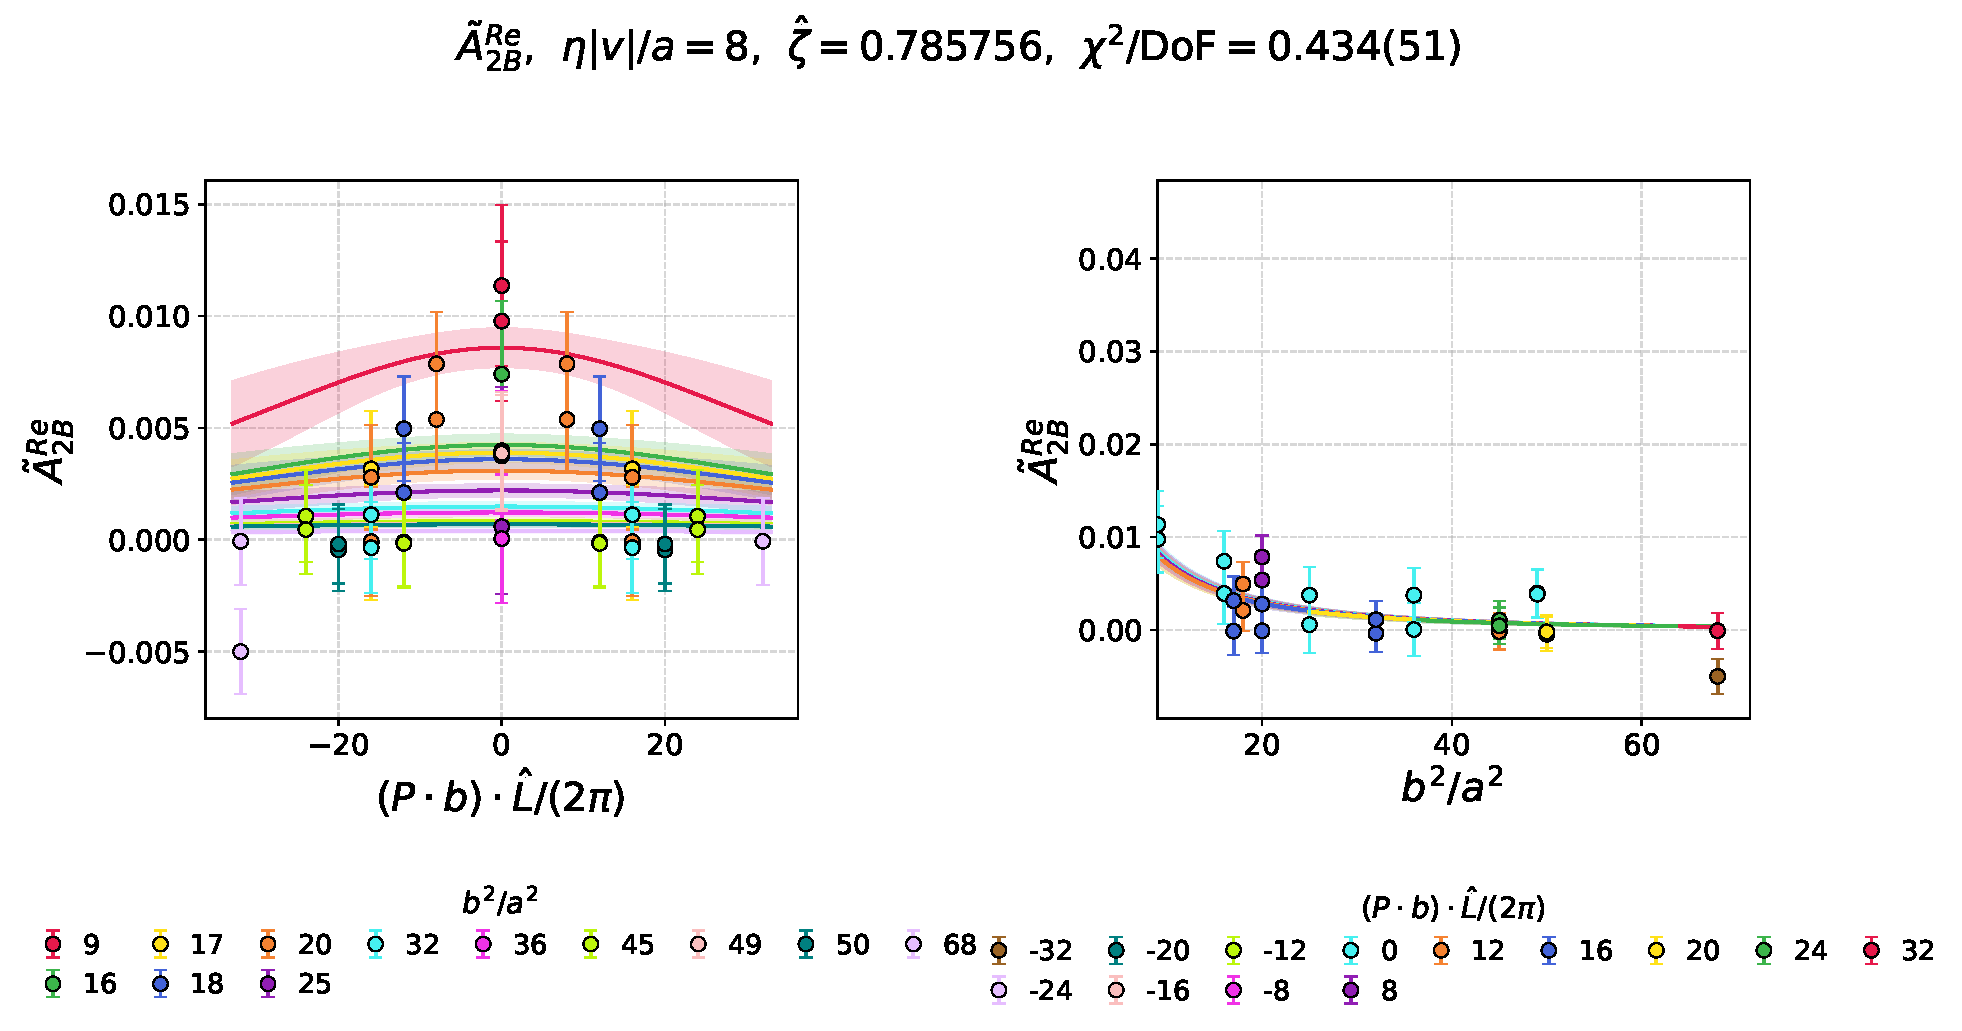
\includegraphics[width=\linewidth,height=.70\textheight,keepaspectratio]{fitting/ReA2B_Pb_bsq_eta8_PL-4_WithFit_2D.pdf}
\par\small Both invariant-coordinate slices. Same simultaneous fit, with Jackknife bands.

\figsrc{Thesis: plots; ReA2B\_Pb\_bsq\_eta8\_PL-4\_WithFit\_2D}
\end{frame}

\begin{frame}{Global fit: $\tAmp_{2B}^{\mathrm{Im}}$, $P_L=-4$}
\centering
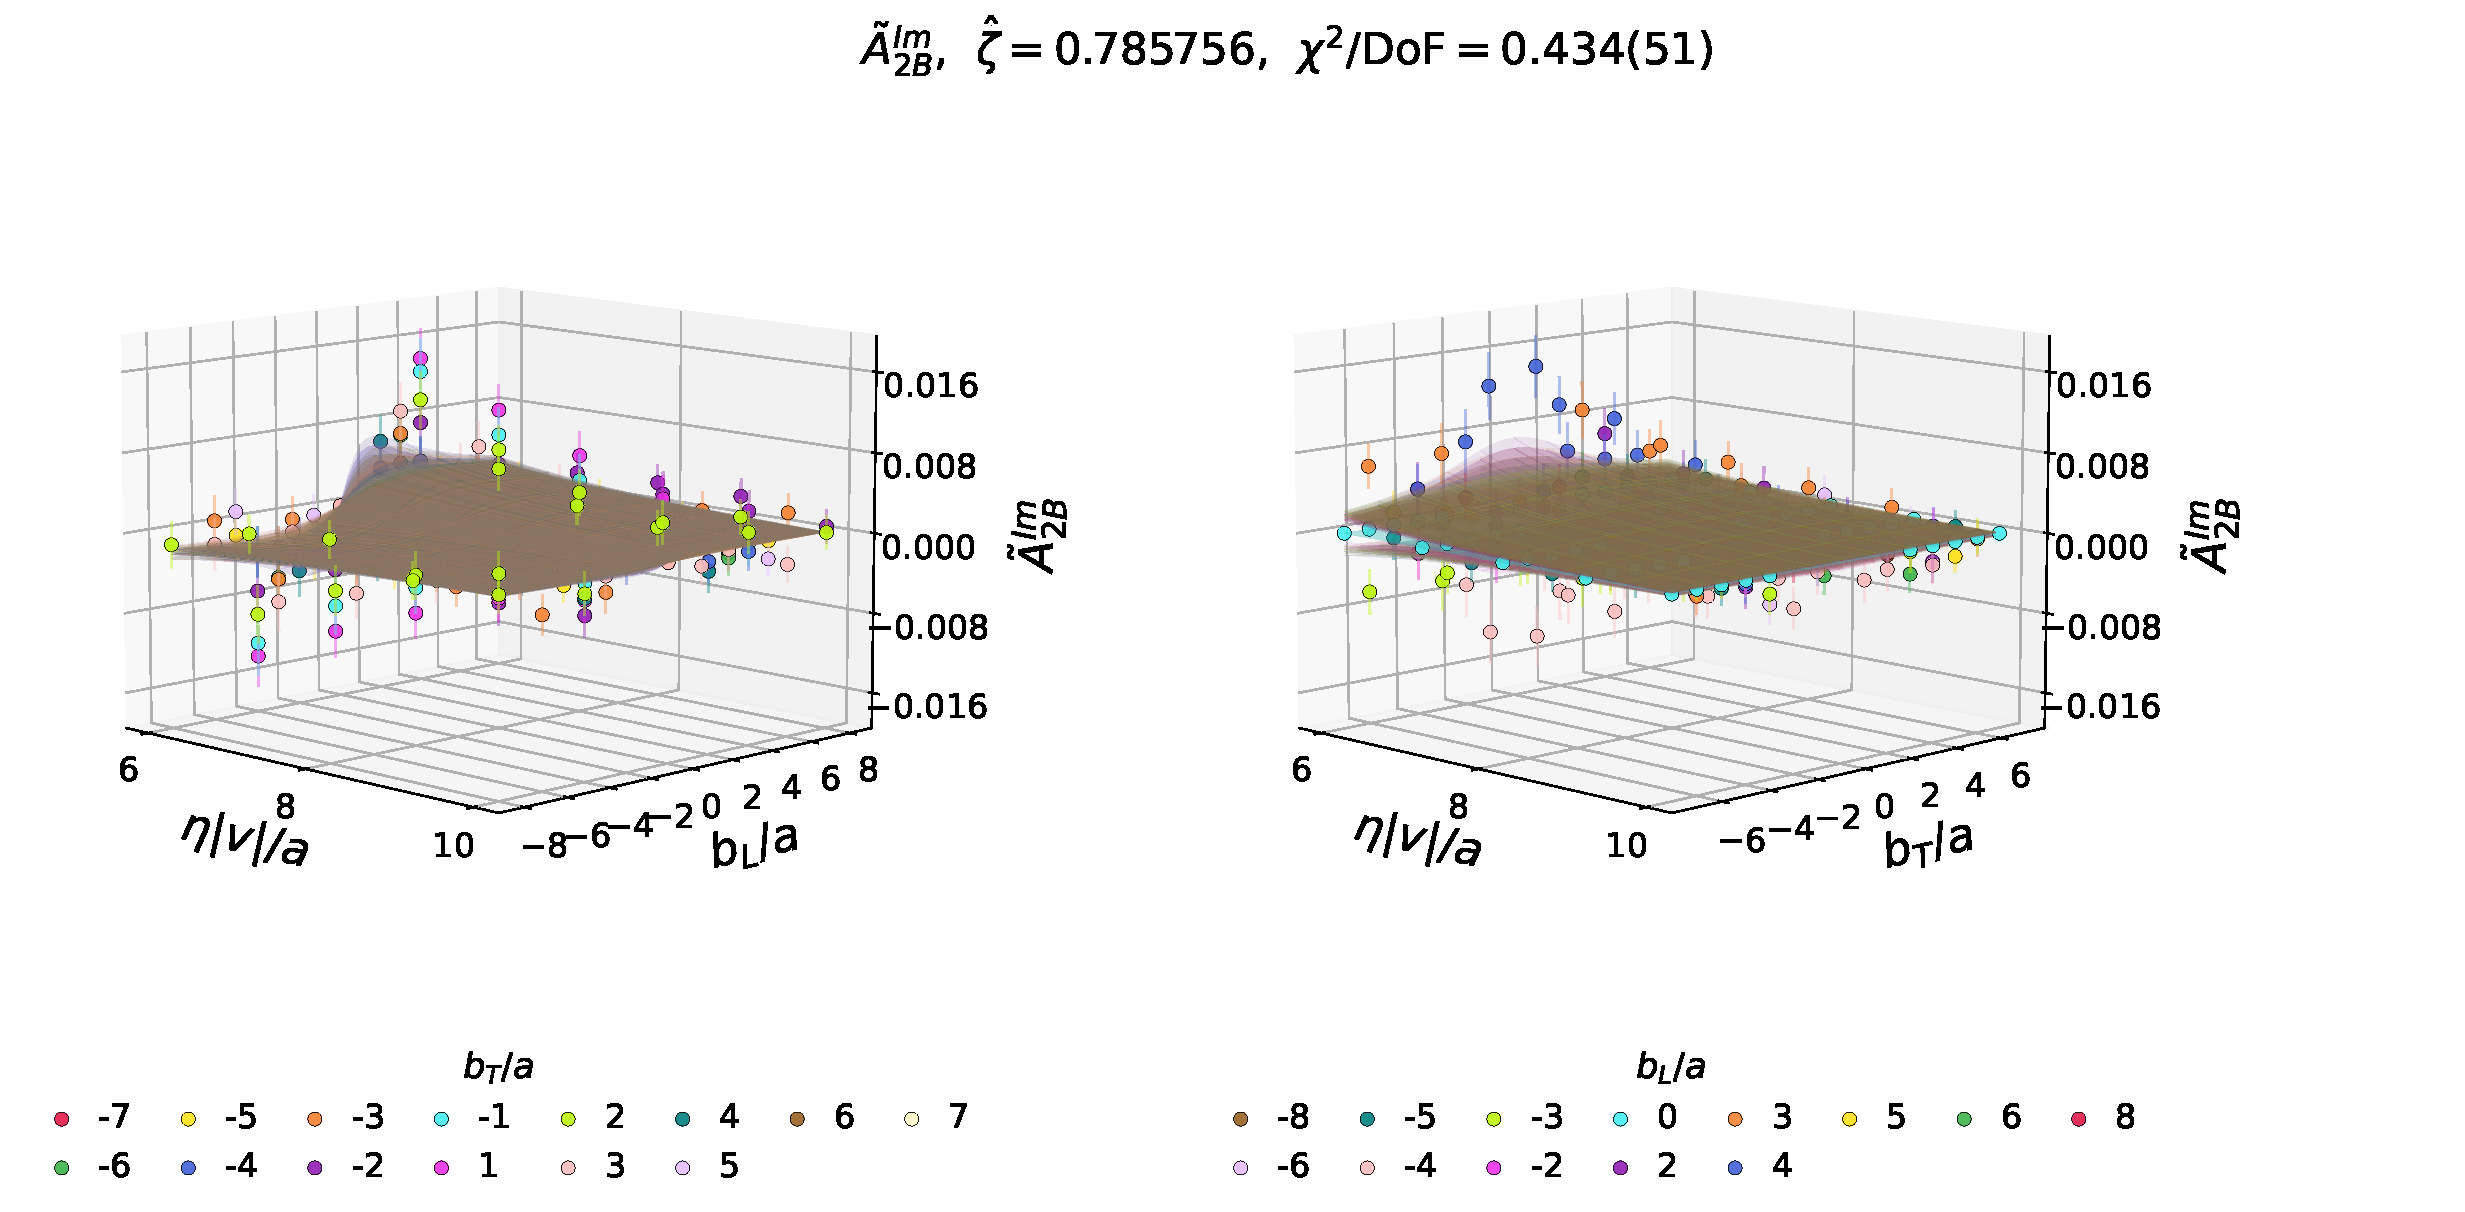
\includegraphics[width=\linewidth,height=.70\textheight,keepaspectratio]{fitting/ImA2B_PL-4_WithFit_3D.pdf}
\par\small Spatial coordinates: $(b_L,b_T,\eta)$. All panels and data overlays retained.

\figsrc{Thesis: plots; ImA2B\_PL-4\_WithFit\_3D}
\end{frame}

\begin{frame}{Global fit: $\tAmp_{2B}^{\mathrm{Im}}$, $P_L=-4$}
\centering
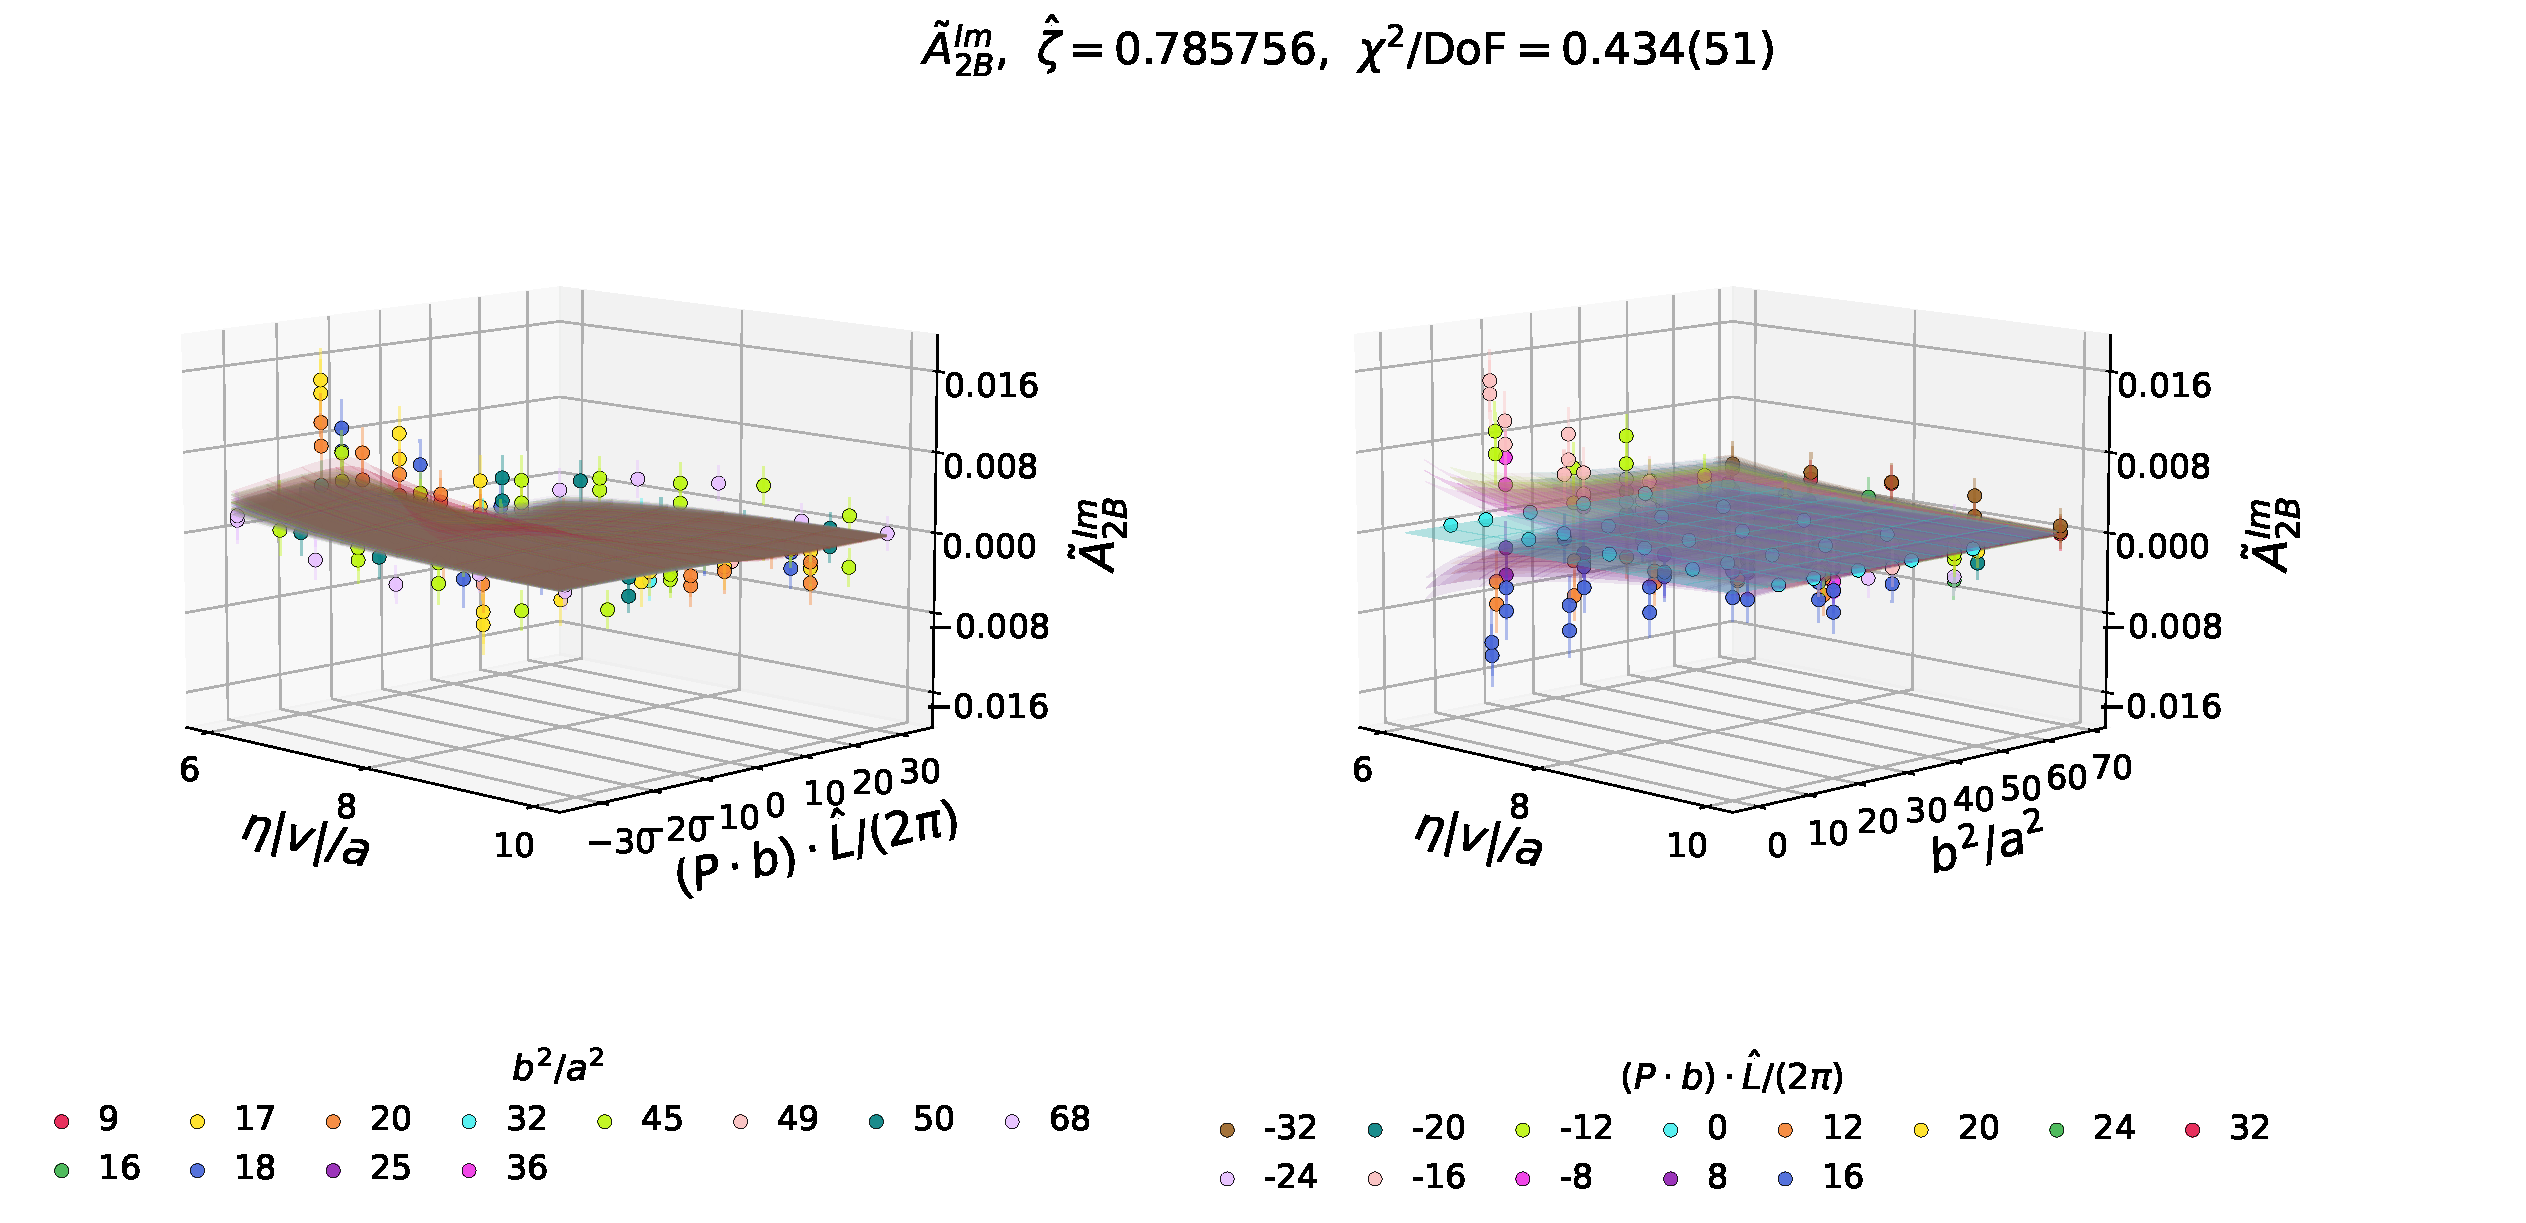
\includegraphics[width=\linewidth,height=.70\textheight,keepaspectratio]{fitting/ImA2B_Pb_bsq_PL-4_WithFit_3D.pdf}
\par\small Invariant coordinates: $(\nu,b^2,\eta)$. All panels and data overlays retained.

\figsrc{Thesis: plots; ImA2B\_Pb\_bsq\_PL-4\_WithFit\_3D}
\end{frame}

\begin{frame}{Fixed staple $\eta=8$: $\tAmp_{2B}^{\mathrm{Im}}$, $P_L=-4$}
\centering
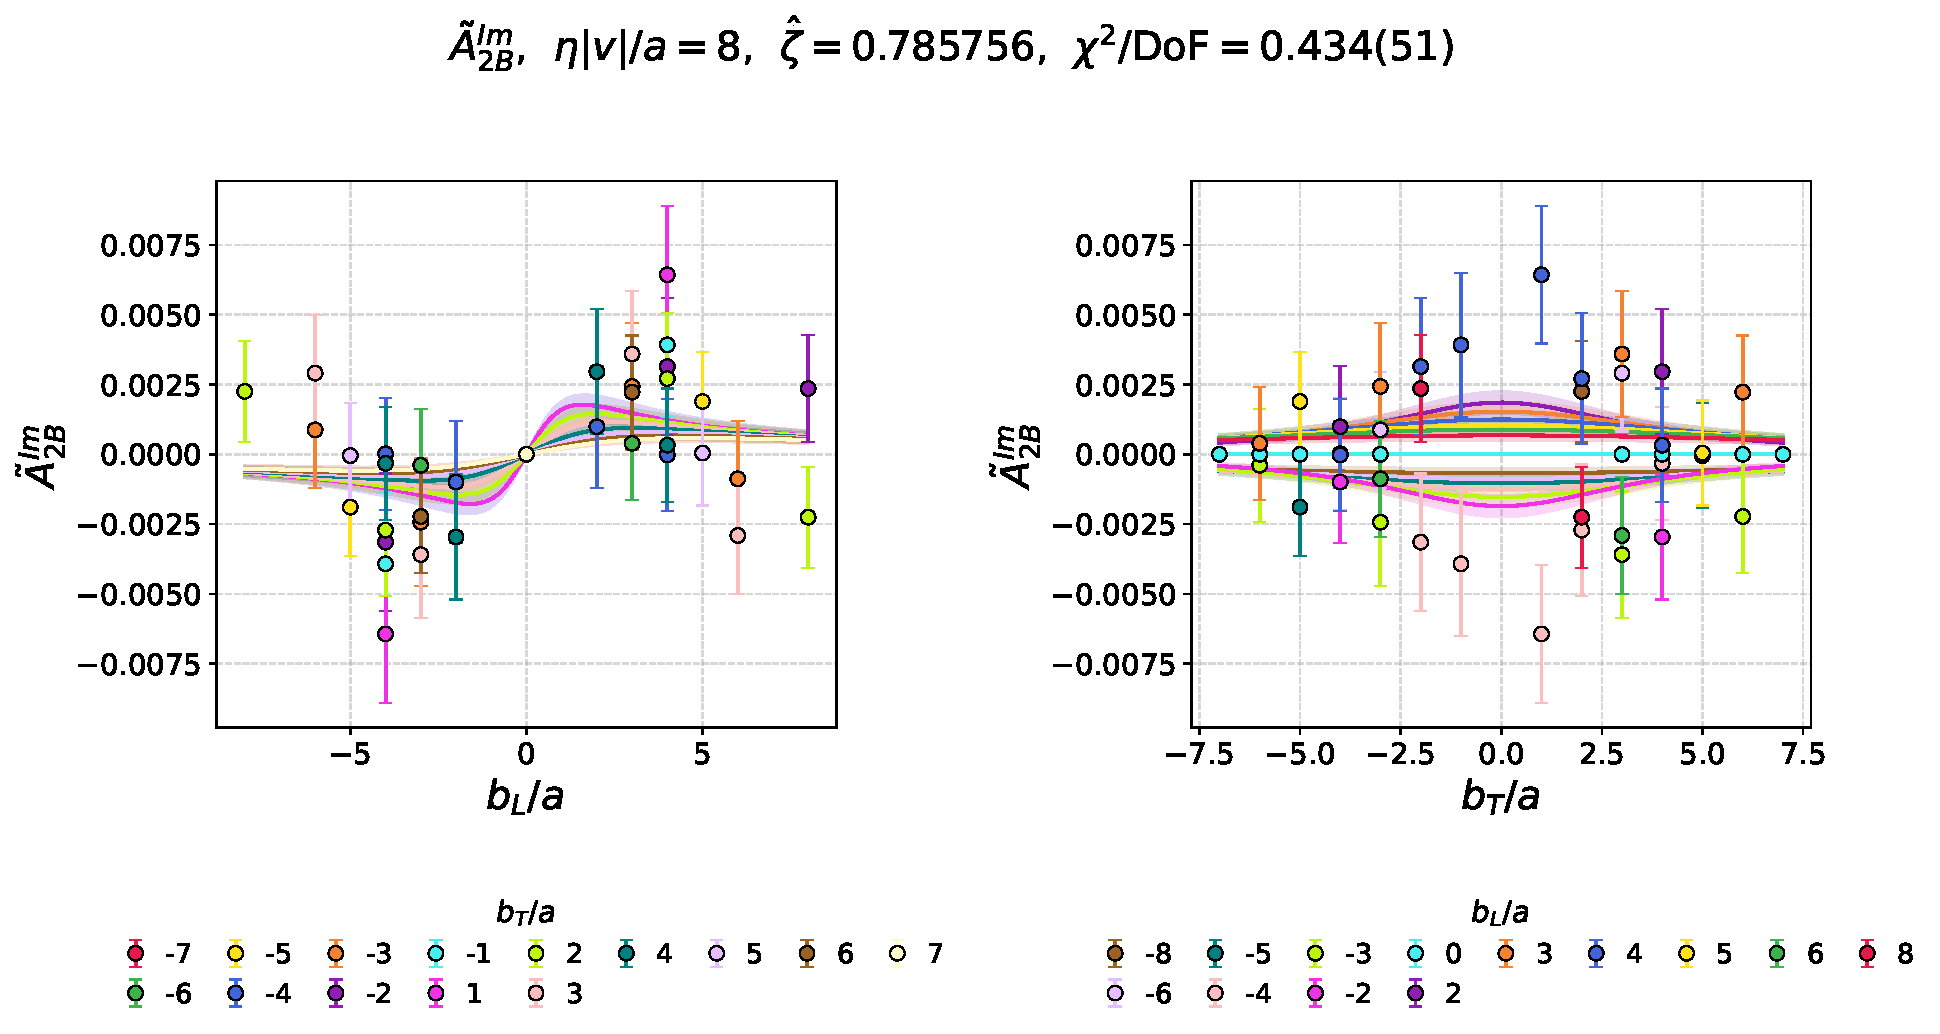
\includegraphics[width=\linewidth,height=.70\textheight,keepaspectratio]{fitting/ImA2B_eta8_PL-4_WithFit_2D.pdf}
\par\small Both spatial-coordinate slices. Same simultaneous fit, with Jackknife bands.

\figsrc{Thesis: plots; ImA2B\_eta8\_PL-4\_WithFit\_2D}
\end{frame}

\begin{frame}{Fixed staple $\eta=8$: $\tAmp_{2B}^{\mathrm{Im}}$, $P_L=-4$}
\centering
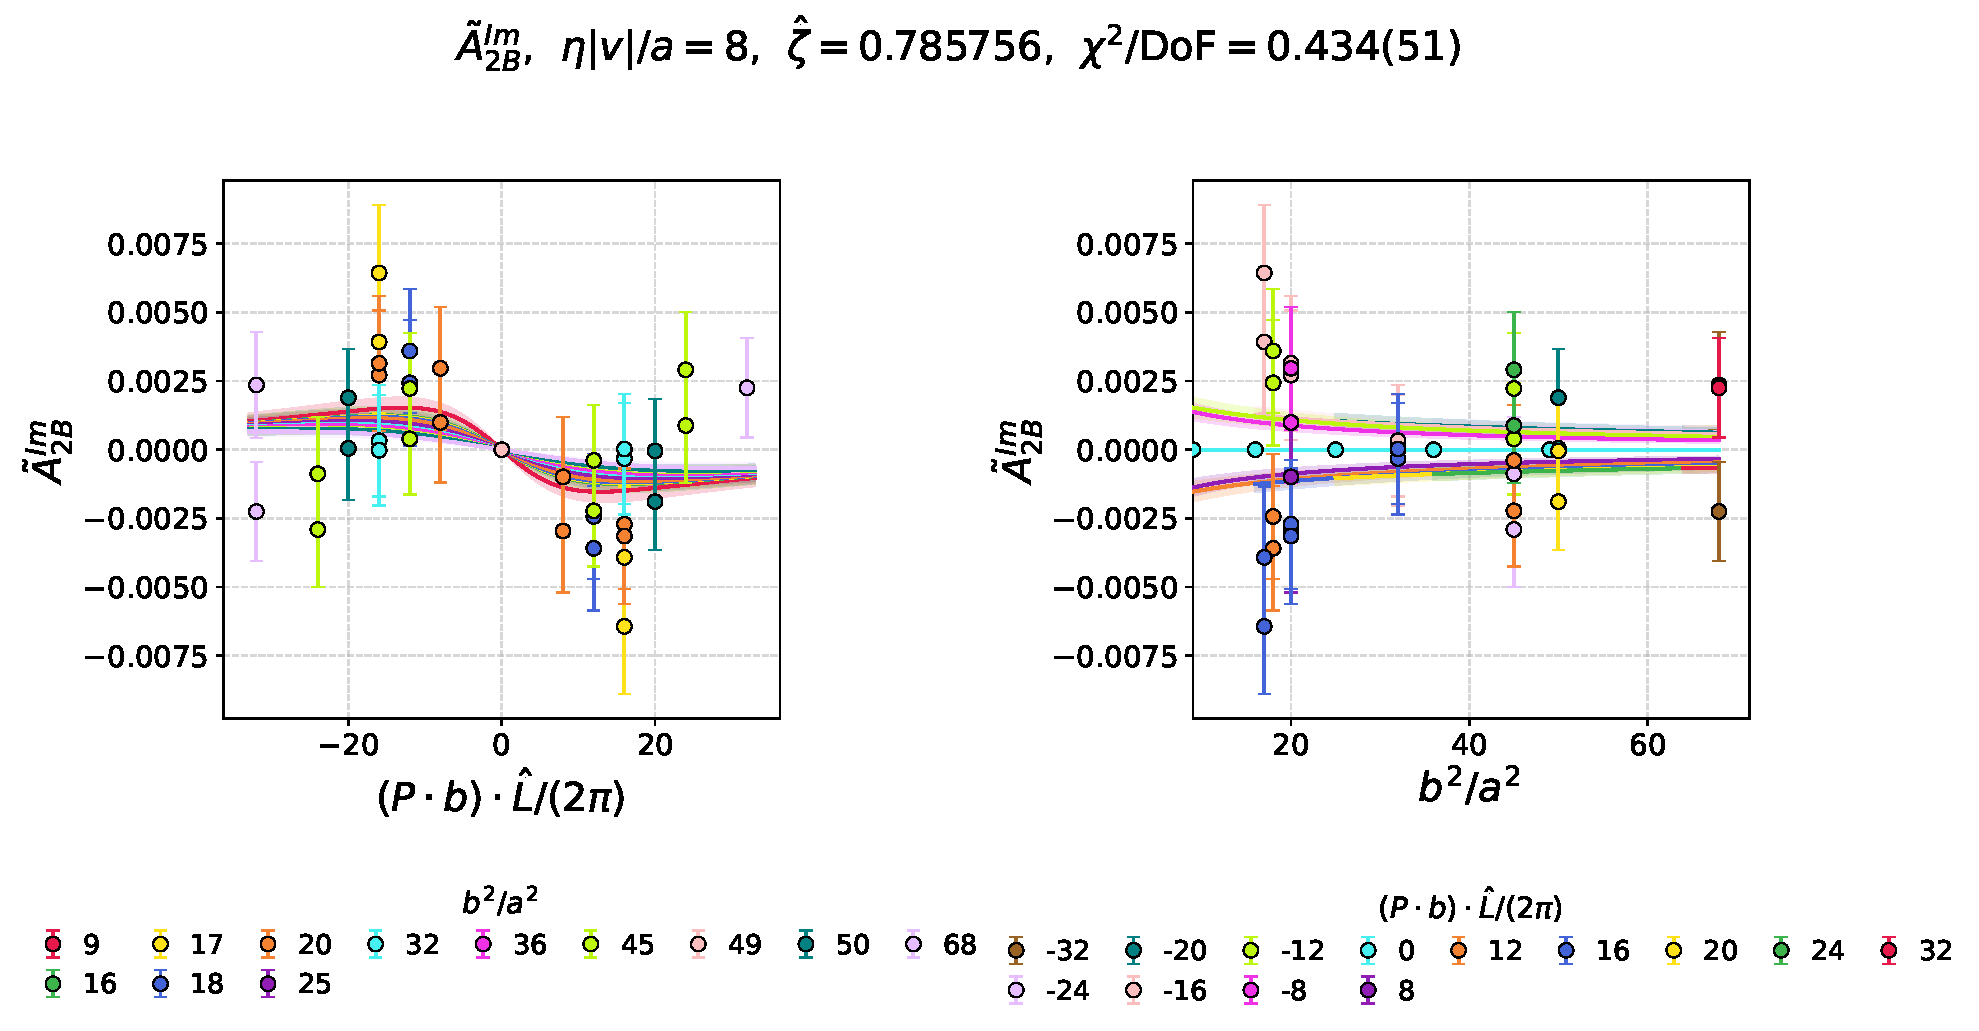
\includegraphics[width=\linewidth,height=.70\textheight,keepaspectratio]{fitting/ImA2B_Pb_bsq_eta8_PL-4_WithFit_2D.pdf}
\par\small Both invariant-coordinate slices. Same simultaneous fit, with Jackknife bands.

\figsrc{Thesis: plots; ImA2B\_Pb\_bsq\_eta8\_PL-4\_WithFit\_2D}
\end{frame}

\begin{frame}{Global fit: $\tAmp_{12B}^{\mathrm{Re}}$, $P_L=-4$}
\centering
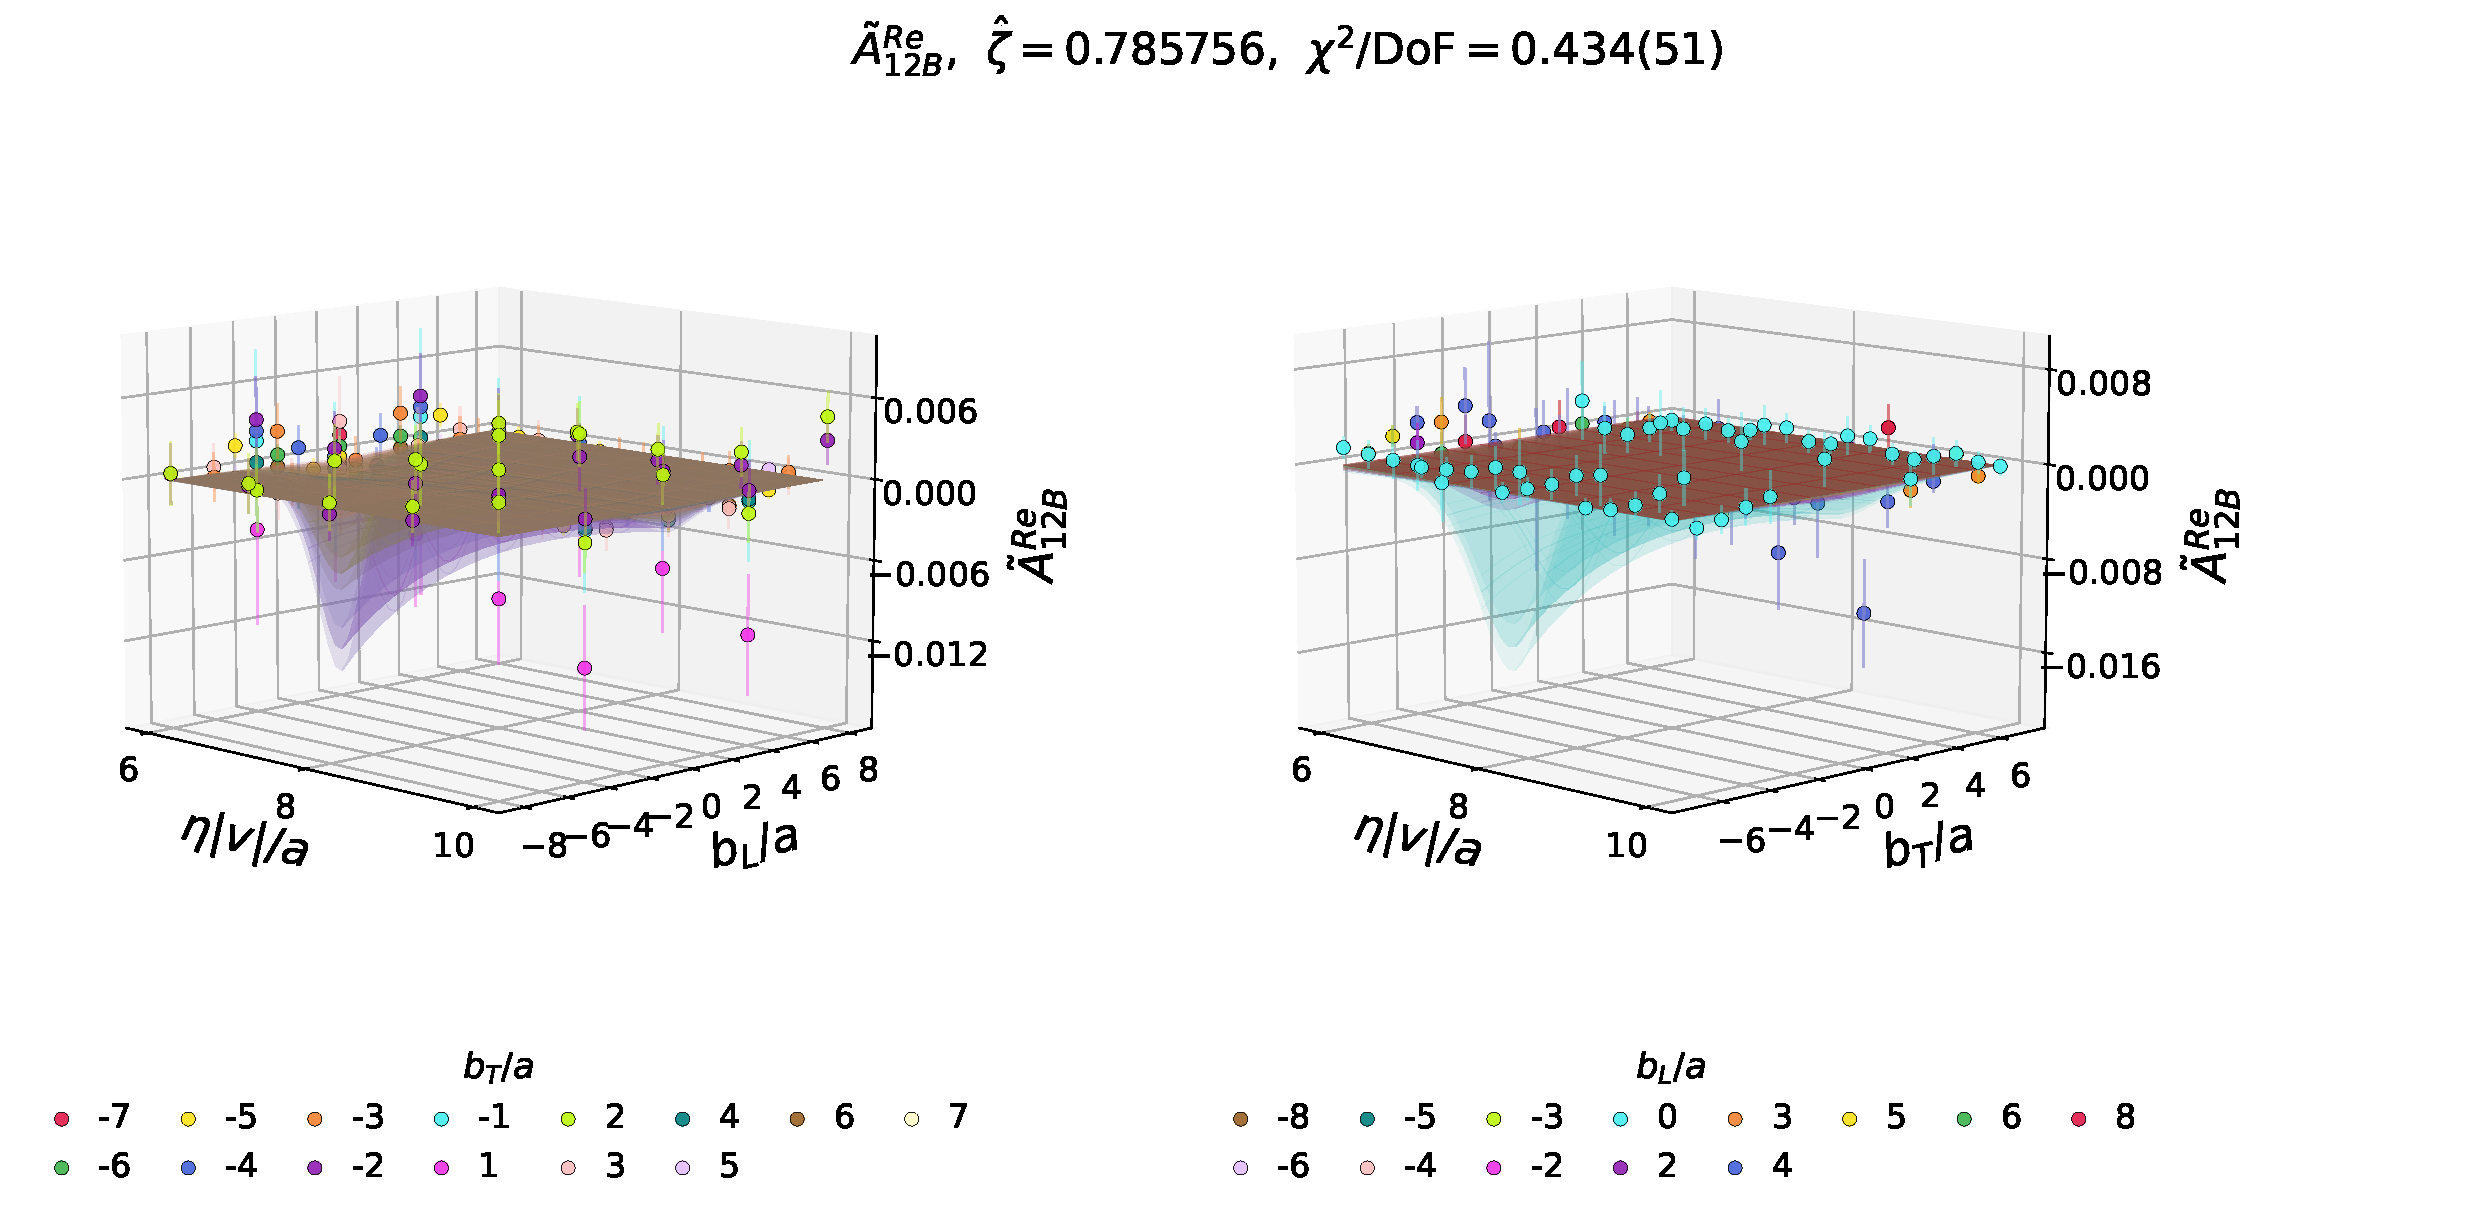
\includegraphics[width=\linewidth,height=.70\textheight,keepaspectratio]{fitting/ReA12B_PL-4_WithFit_3D.pdf}
\par\small Spatial coordinates: $(b_L,b_T,\eta)$. All panels and data overlays retained.

\figsrc{Thesis: plots; ReA12B\_PL-4\_WithFit\_3D}
\end{frame}

\begin{frame}{Global fit: $\tAmp_{12B}^{\mathrm{Re}}$, $P_L=-4$}
\centering
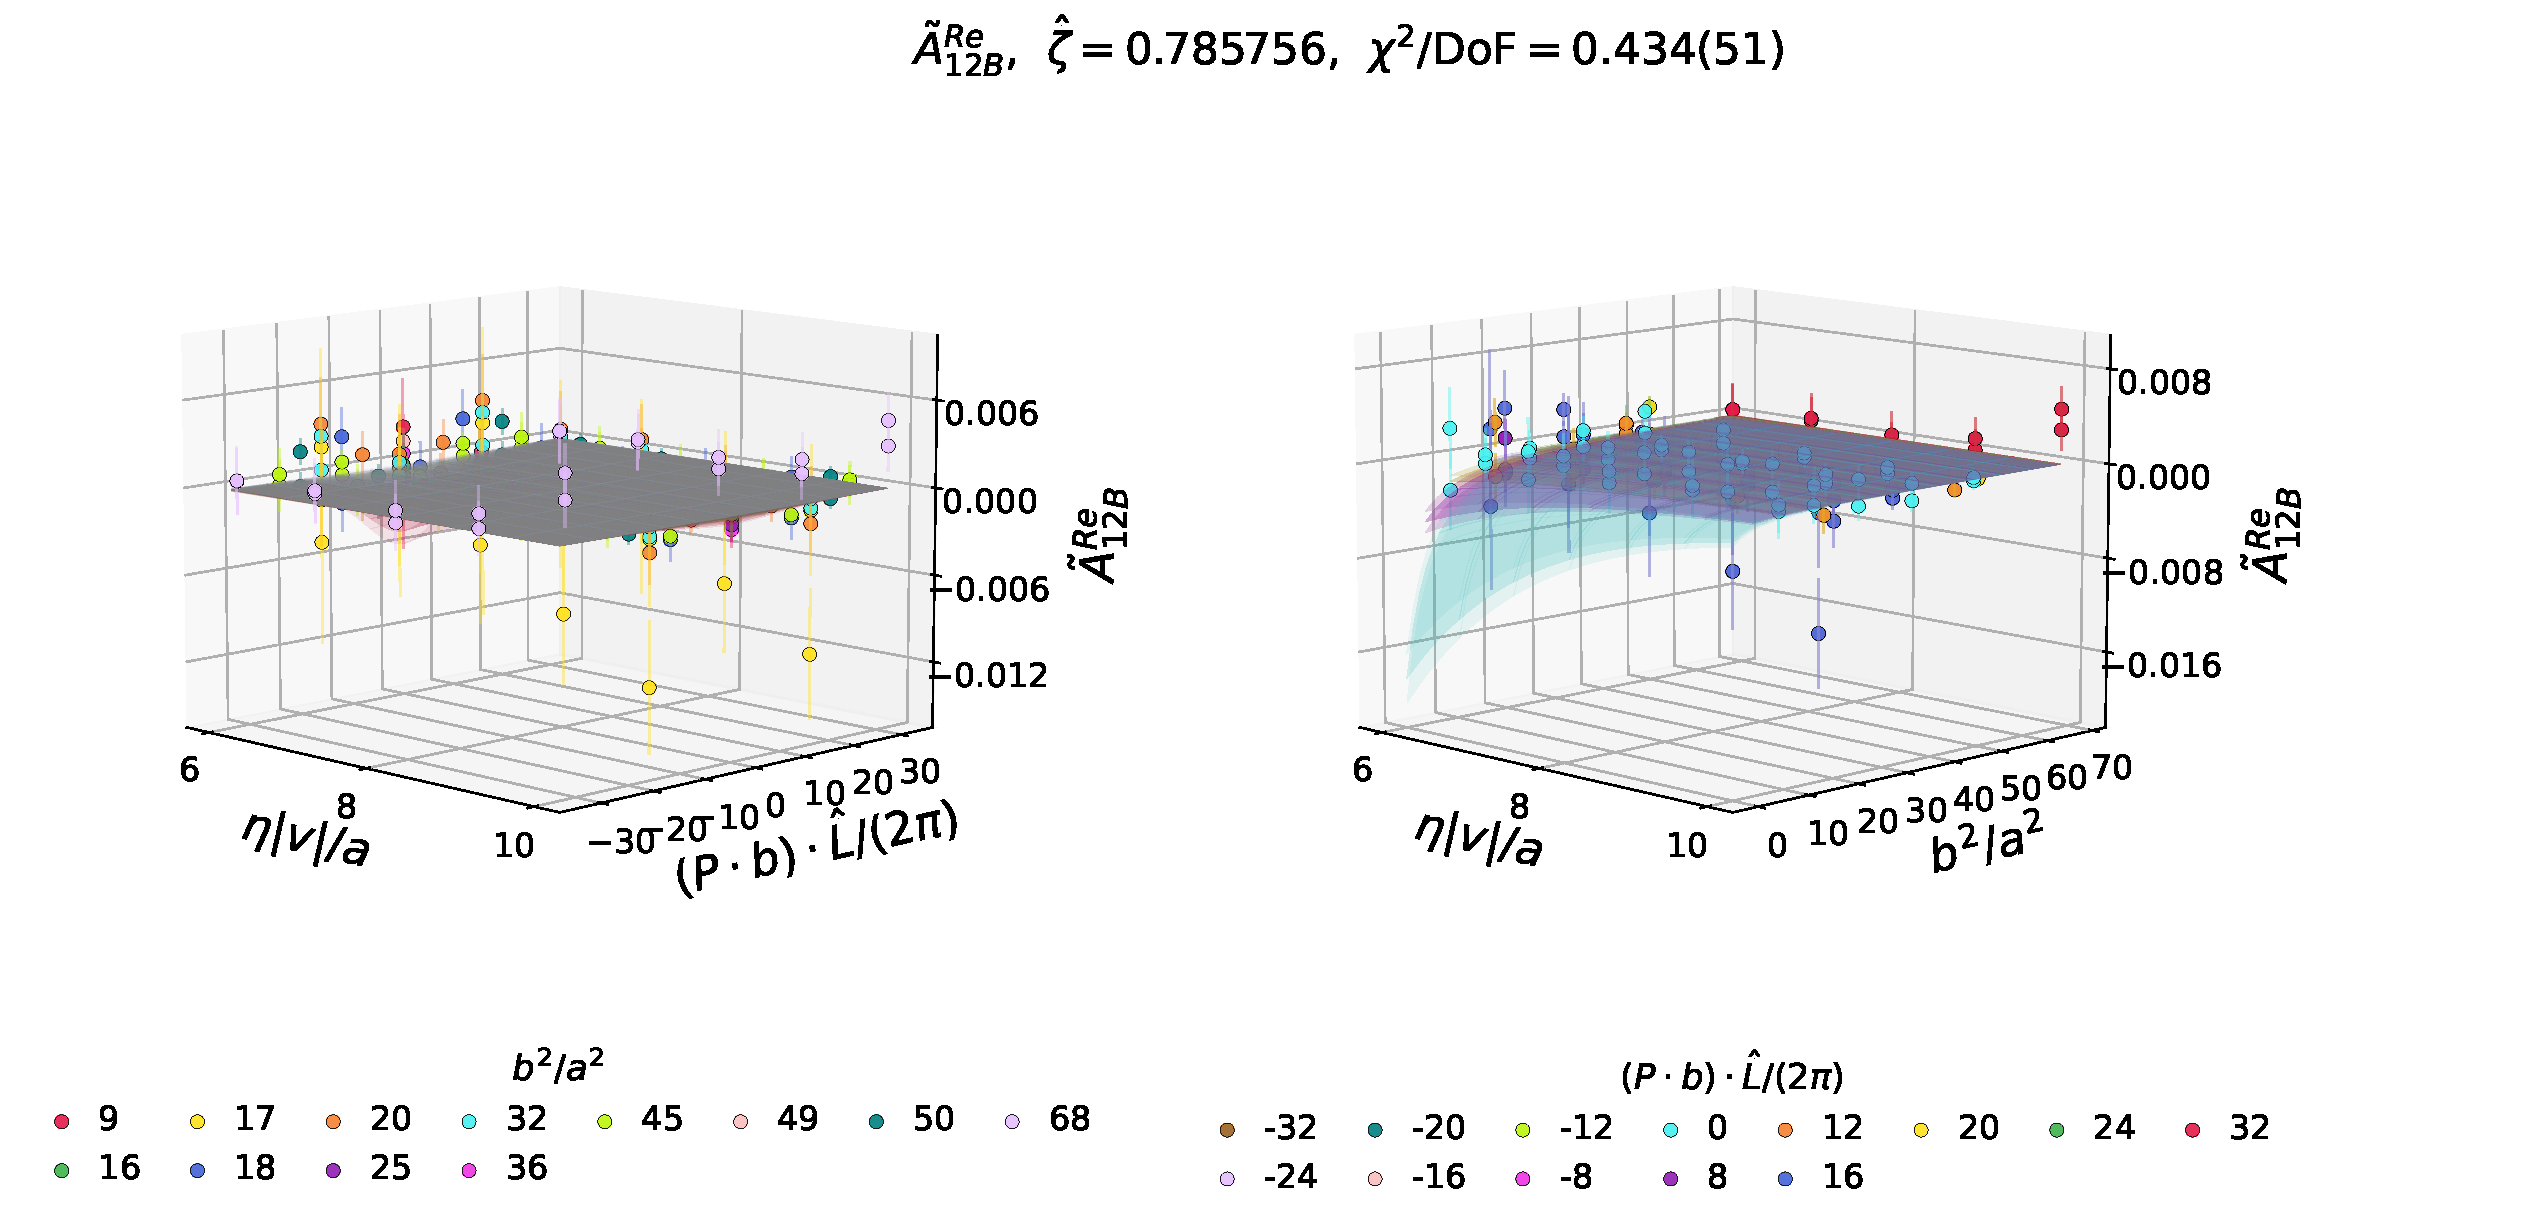
\includegraphics[width=\linewidth,height=.70\textheight,keepaspectratio]{fitting/ReA12B_Pb_bsq_PL-4_WithFit_3D.pdf}
\par\small Invariant coordinates: $(\nu,b^2,\eta)$. All panels and data overlays retained.

\figsrc{Thesis: plots; ReA12B\_Pb\_bsq\_PL-4\_WithFit\_3D}
\end{frame}

\begin{frame}{Fixed staple $\eta=8$: $\tAmp_{12B}^{\mathrm{Re}}$, $P_L=-4$}
\centering
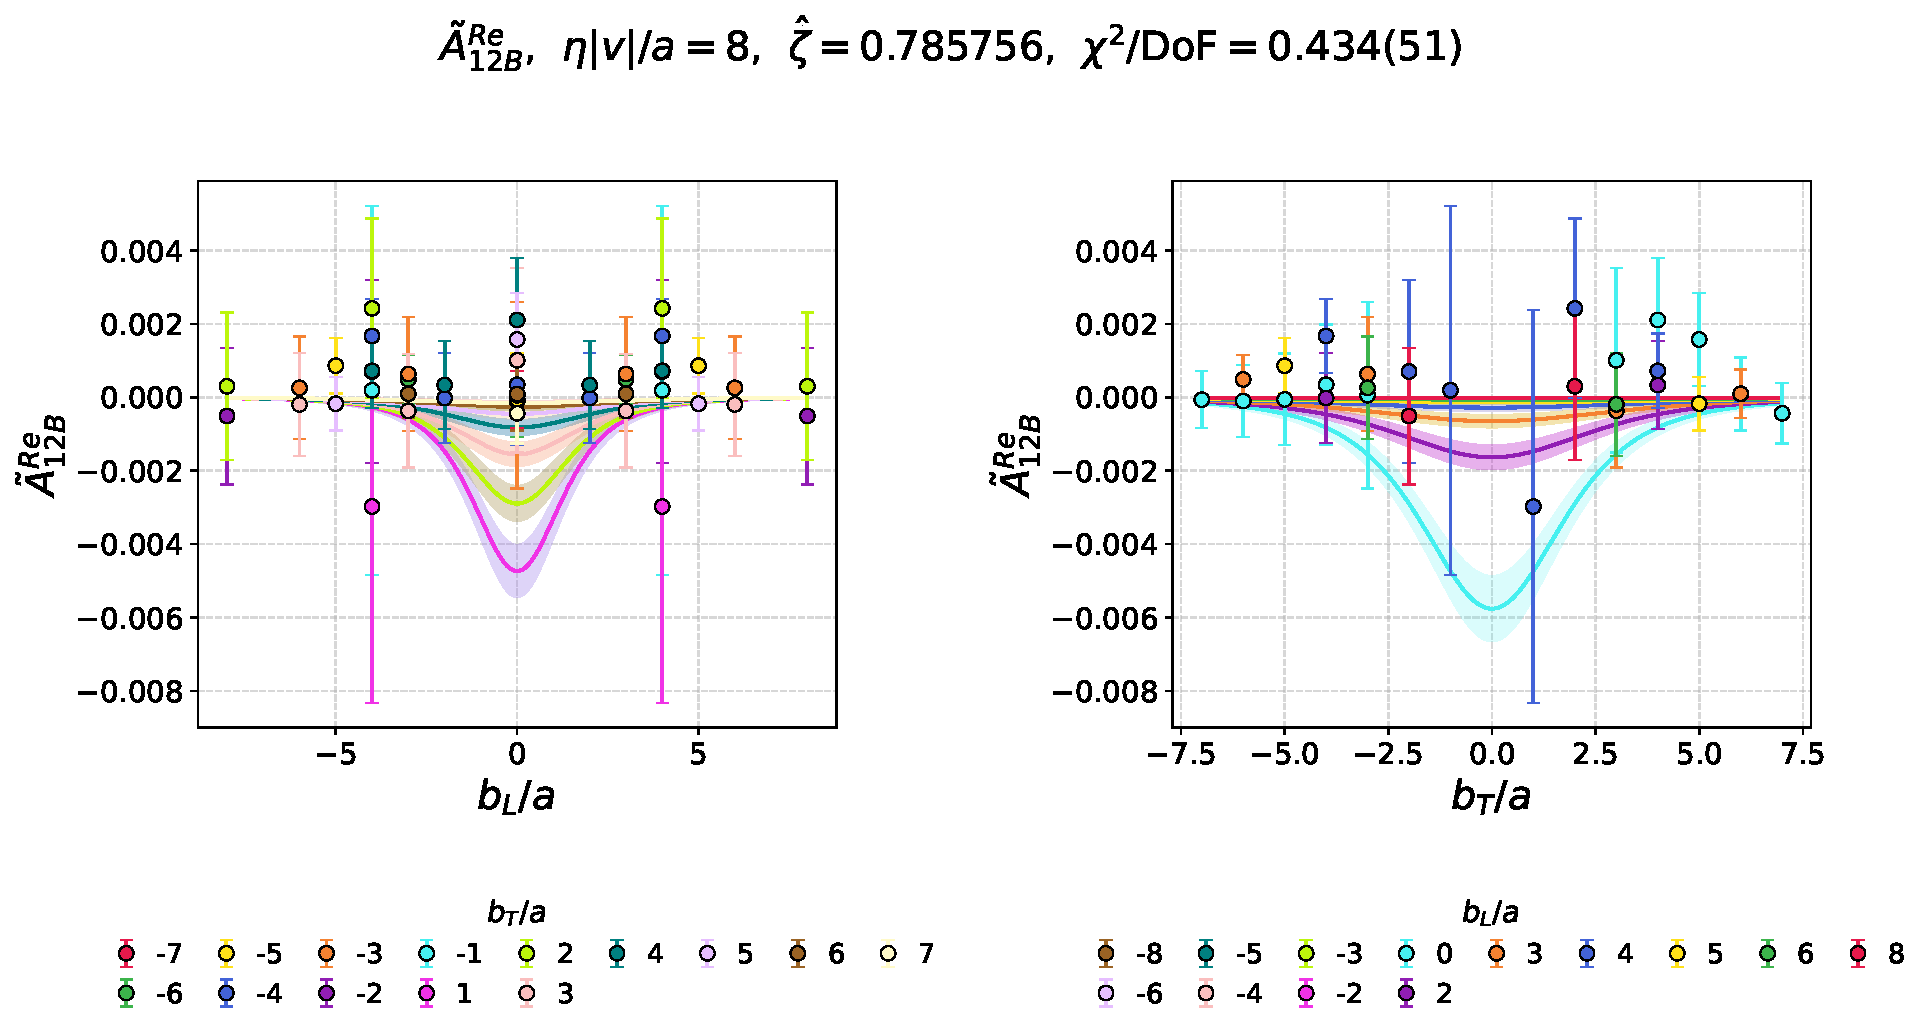
\includegraphics[width=\linewidth,height=.70\textheight,keepaspectratio]{fitting/ReA12B_eta8_PL-4_WithFit_2D.pdf}
\par\small Both spatial-coordinate slices. Same simultaneous fit, with Jackknife bands.

\figsrc{Thesis: plots; ReA12B\_eta8\_PL-4\_WithFit\_2D}
\end{frame}

\begin{frame}{Fixed staple $\eta=8$: $\tAmp_{12B}^{\mathrm{Re}}$, $P_L=-4$}
\centering
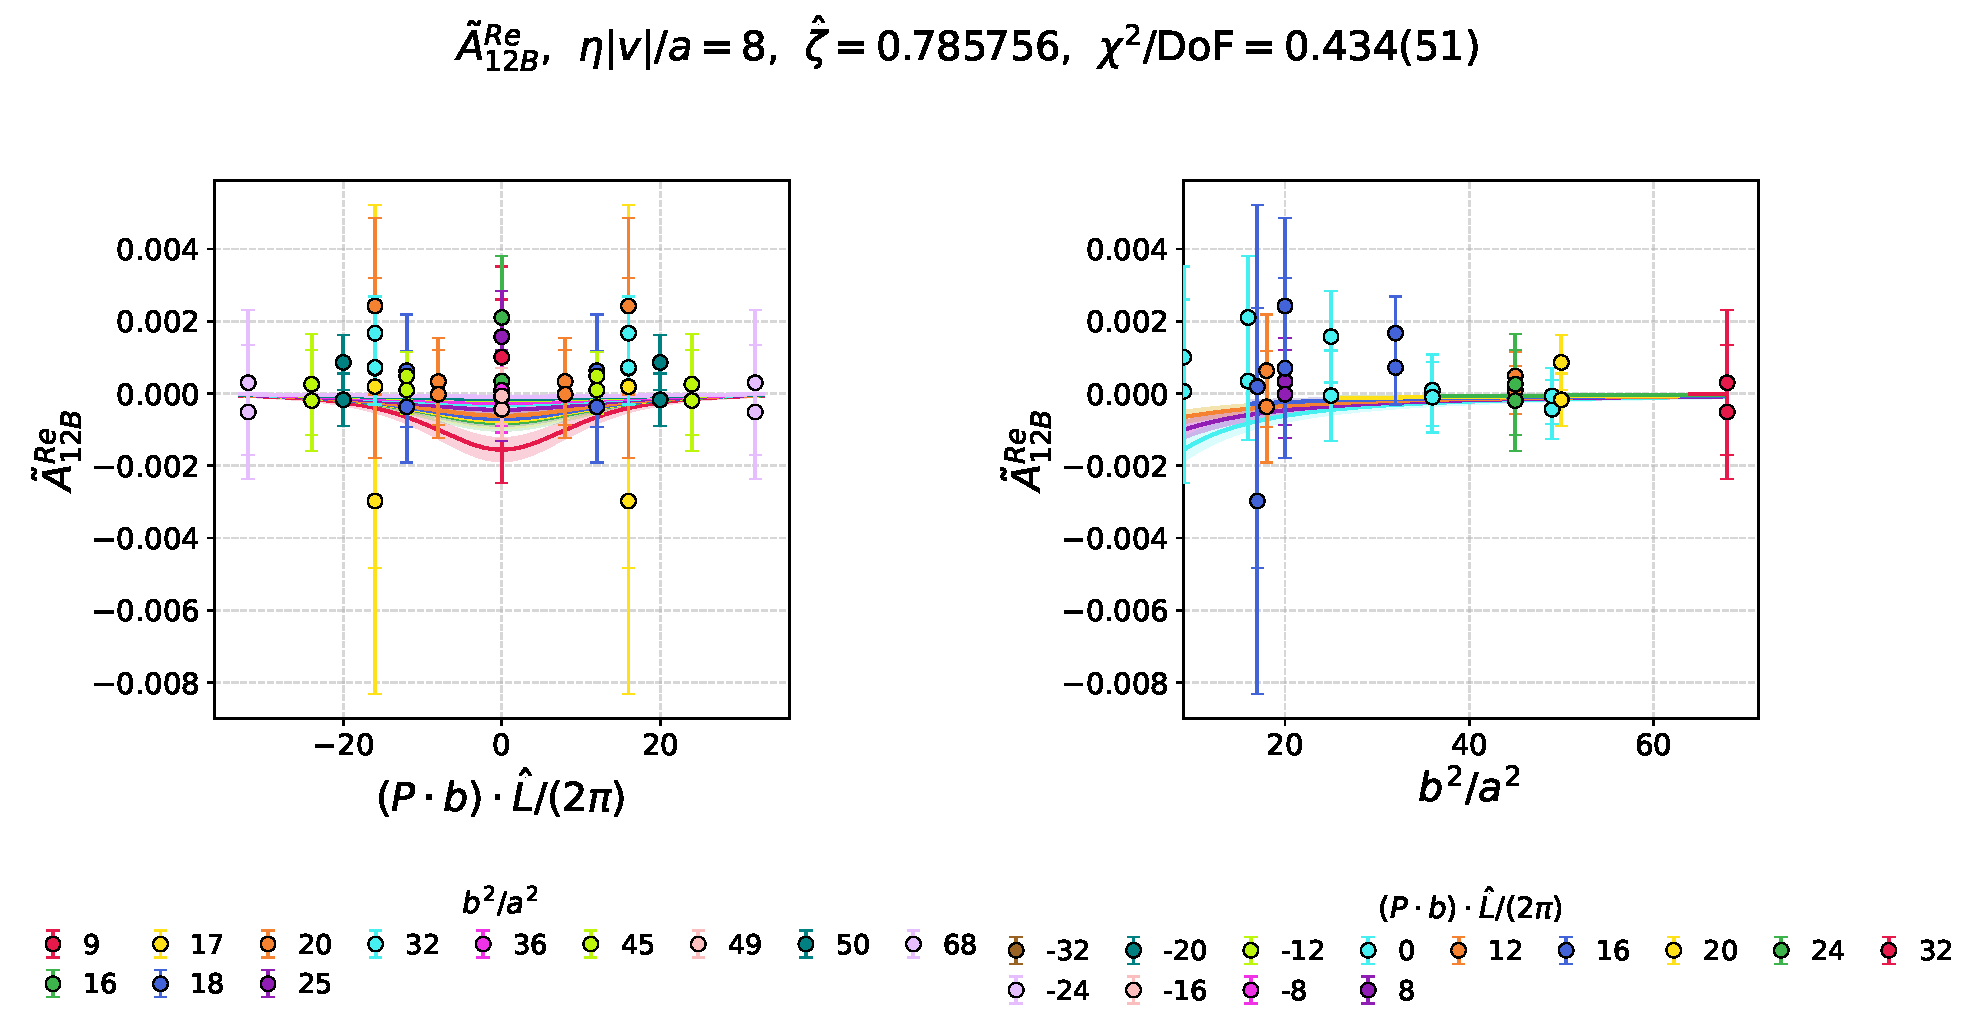
\includegraphics[width=\linewidth,height=.70\textheight,keepaspectratio]{fitting/ReA12B_Pb_bsq_eta8_PL-4_WithFit_2D.pdf}
\par\small Both invariant-coordinate slices. Same simultaneous fit, with Jackknife bands.

\figsrc{Thesis: plots; ReA12B\_Pb\_bsq\_eta8\_PL-4\_WithFit\_2D}
\end{frame}

\begin{frame}{Integrated Fourier results: $P_L=-4$}
\small\renewcommand{\arraystretch}{1.8}\begin{tabular}{lcccc}\toprule Integral & $(-\infty,\infty)$ & $[-1,1]$ & $[-1,0]$ & $[0,1]$\\\midrule
$\int dx\,E$ & 0.87(10) & 0.87(10) & 0.434(52) & 0.434(52) \\
$\int dx\,O$ & 3(207)e-17 & 2(21)e-16 & 0.153(26) & -0.154(26) \\
$\int dx\,\tilde f_1^{(0)}$ & 1.74(21) & 1.74(21) & 0.56(12) & 1.18(12) \\
$\int dx\,\tilde f_{1T}^{\perp(1)}$ & 0.315(55) & 0.315(55) & 0.157(28) & 0.157(28) \\
$m_N\int dx\,\tilde f_{1T}^{\perp(1)}/\int dx\,\tilde f_1^{(0)}$ & 0.195(37) & 0.195(37) & 0.301(73) & 0.144(27) \\
\bottomrule\end{tabular}\par\medskip $b^2=9a^2$; all values and Jackknife uncertainties retained. Numerical values retain the source normalization. The last row is in GeV.
\figsrc{Thesis: SimultaneousFitsCov/Integration\_Table\_PL-4\_bmin3\_b2-9.tex}
\end{frame}

\begin{frame}{Fourier results (2D): $P_L=-4$, unpolarized}
\centering
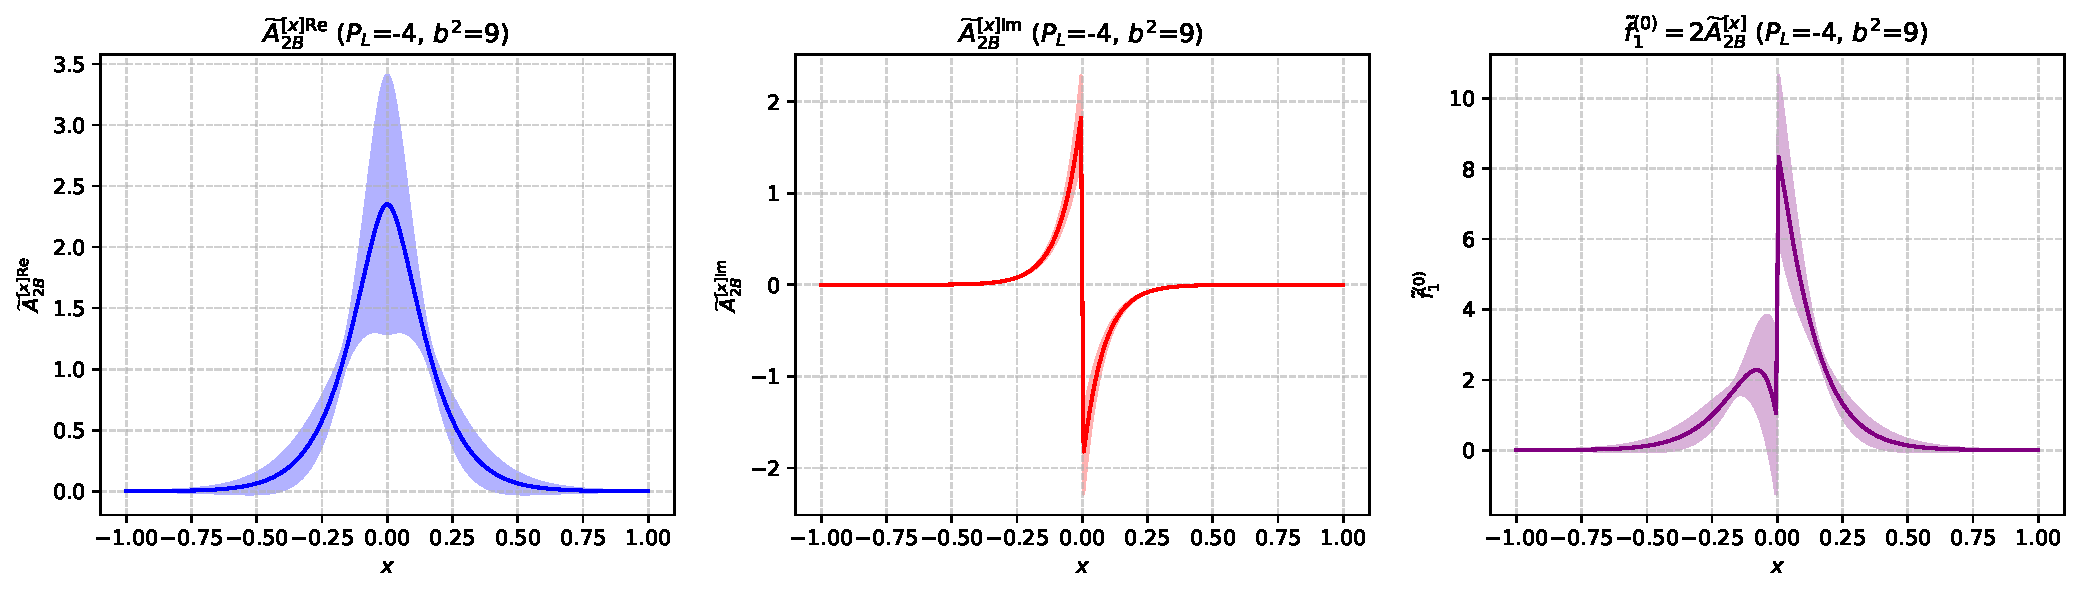
\includegraphics[width=\linewidth,height=.70\textheight,keepaspectratio]{fitting/FT_xdep_A2B_A12B_bmin3_eta610_b2-9_PL-4__row1.pdf}
\par\small Even, odd, and unpolarized transforms. Fixed $b^2=9a^2$.

\figsrc{Thesis: SimultaneousFitsCov; FT\_xdep\_A2B\_A12B\_bmin3\_eta610\_b2-9\_PL-4}
\end{frame}

\begin{frame}{Fourier results (2D): $P_L=-4$, Sivers}
\centering
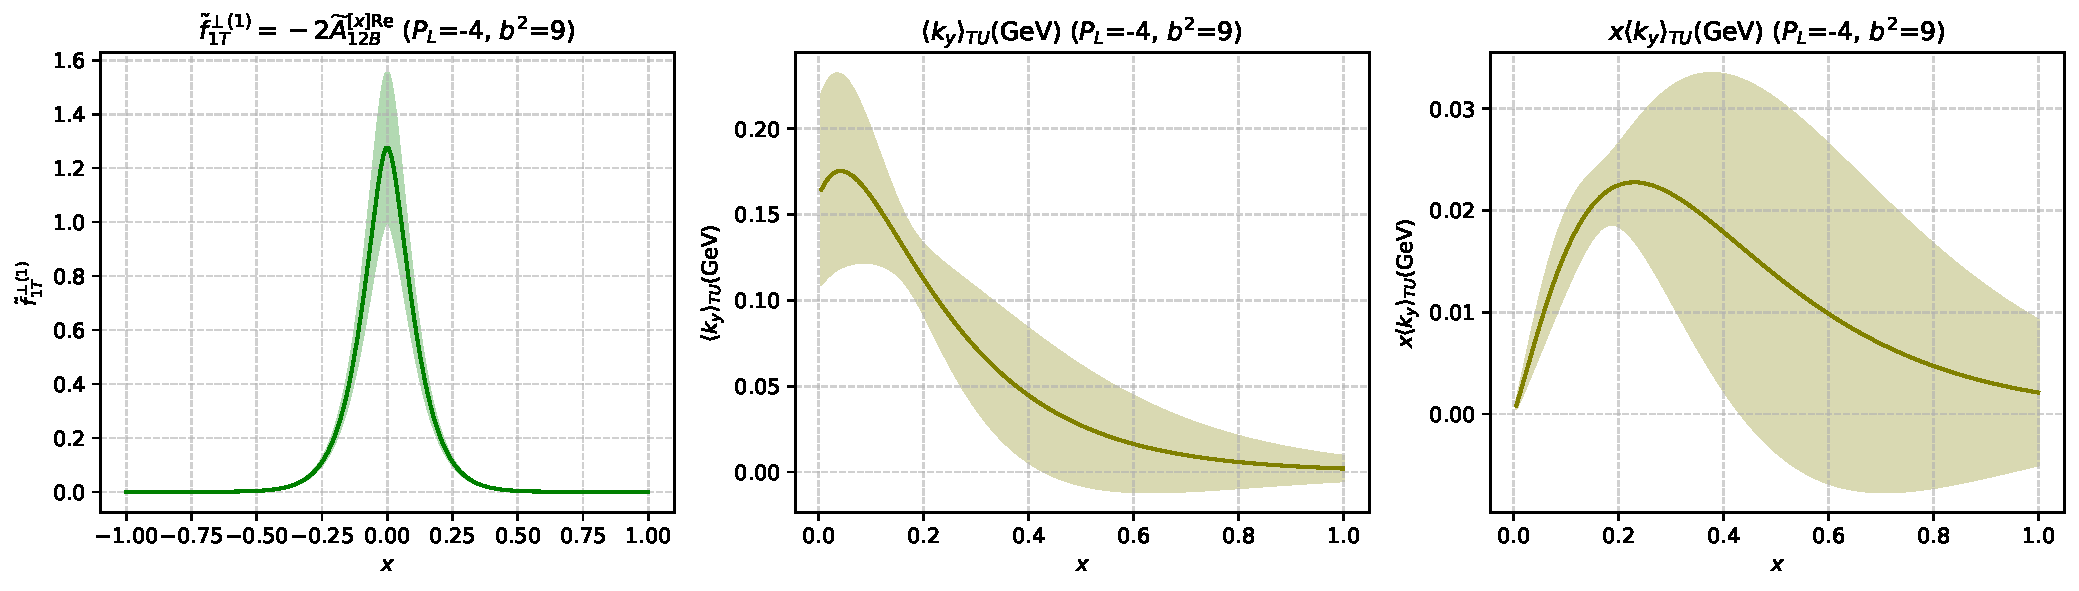
\includegraphics[width=\linewidth,height=.70\textheight,keepaspectratio]{fitting/FT_xdep_A2B_A12B_bmin3_eta610_b2-9_PL-4__row2.pdf}
\par\small Sivers transform, shift, and $x\langle k_y\rangle_{TU}$. Fixed $b^2=9a^2$.

\figsrc{Thesis: SimultaneousFitsCov; FT\_xdep\_A2B\_A12B\_bmin3\_eta610\_b2-9\_PL-4}
\end{frame}

\begin{frame}{Fourier results (3D): $P_L=-4$, unpolarized}
\centering
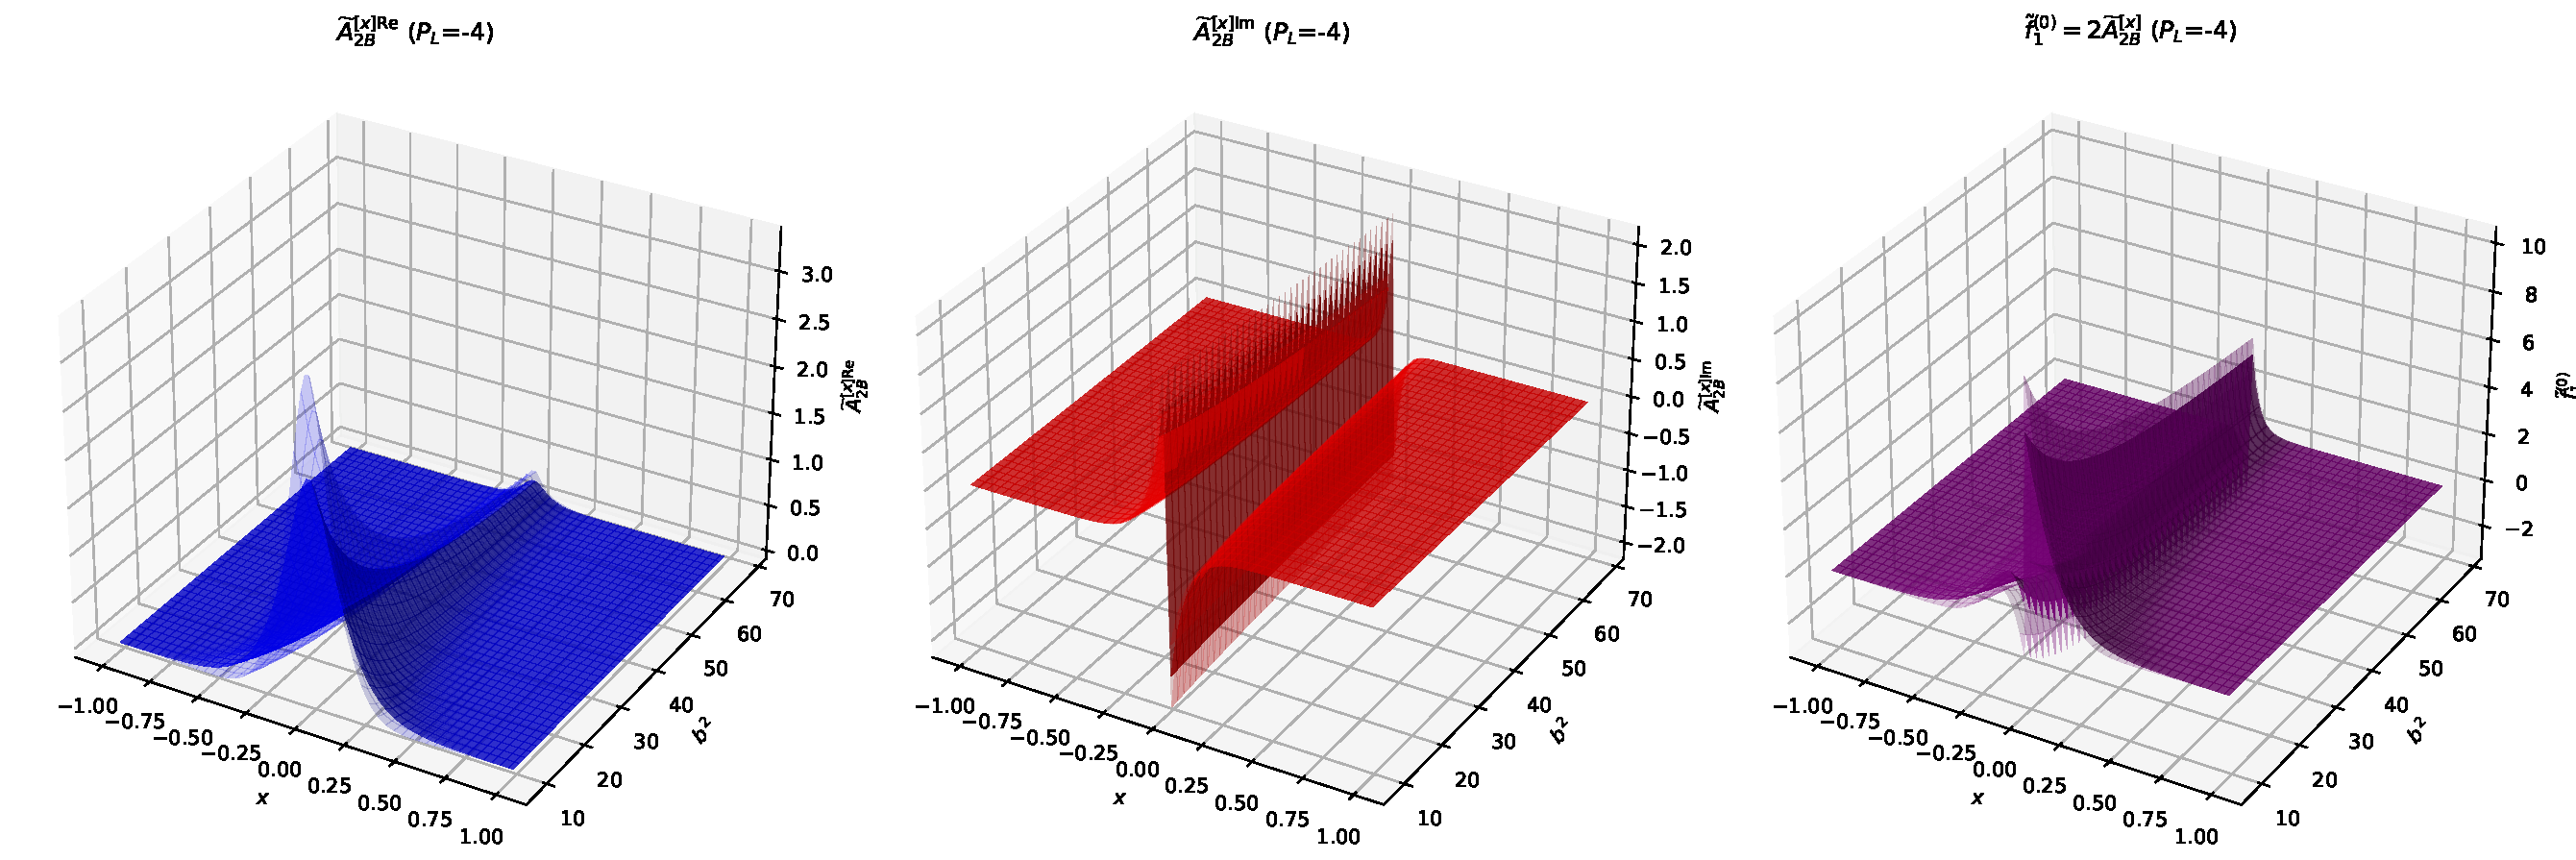
\includegraphics[width=\linewidth,height=.70\textheight,keepaspectratio]{fitting/FT_xdep_3D_A2B_A12B_bmin3_eta610_PL-4__row1.pdf}
\par\small Even, odd, and unpolarized transforms. Full $b^2/a^2\in[9,68]$ dependence.

\figsrc{Thesis: SimultaneousFitsCov; FT\_xdep\_3D\_A2B\_A12B\_bmin3\_eta610\_PL-4}
\end{frame}

\begin{frame}{Fourier results (3D): $P_L=-4$, Sivers}
\centering
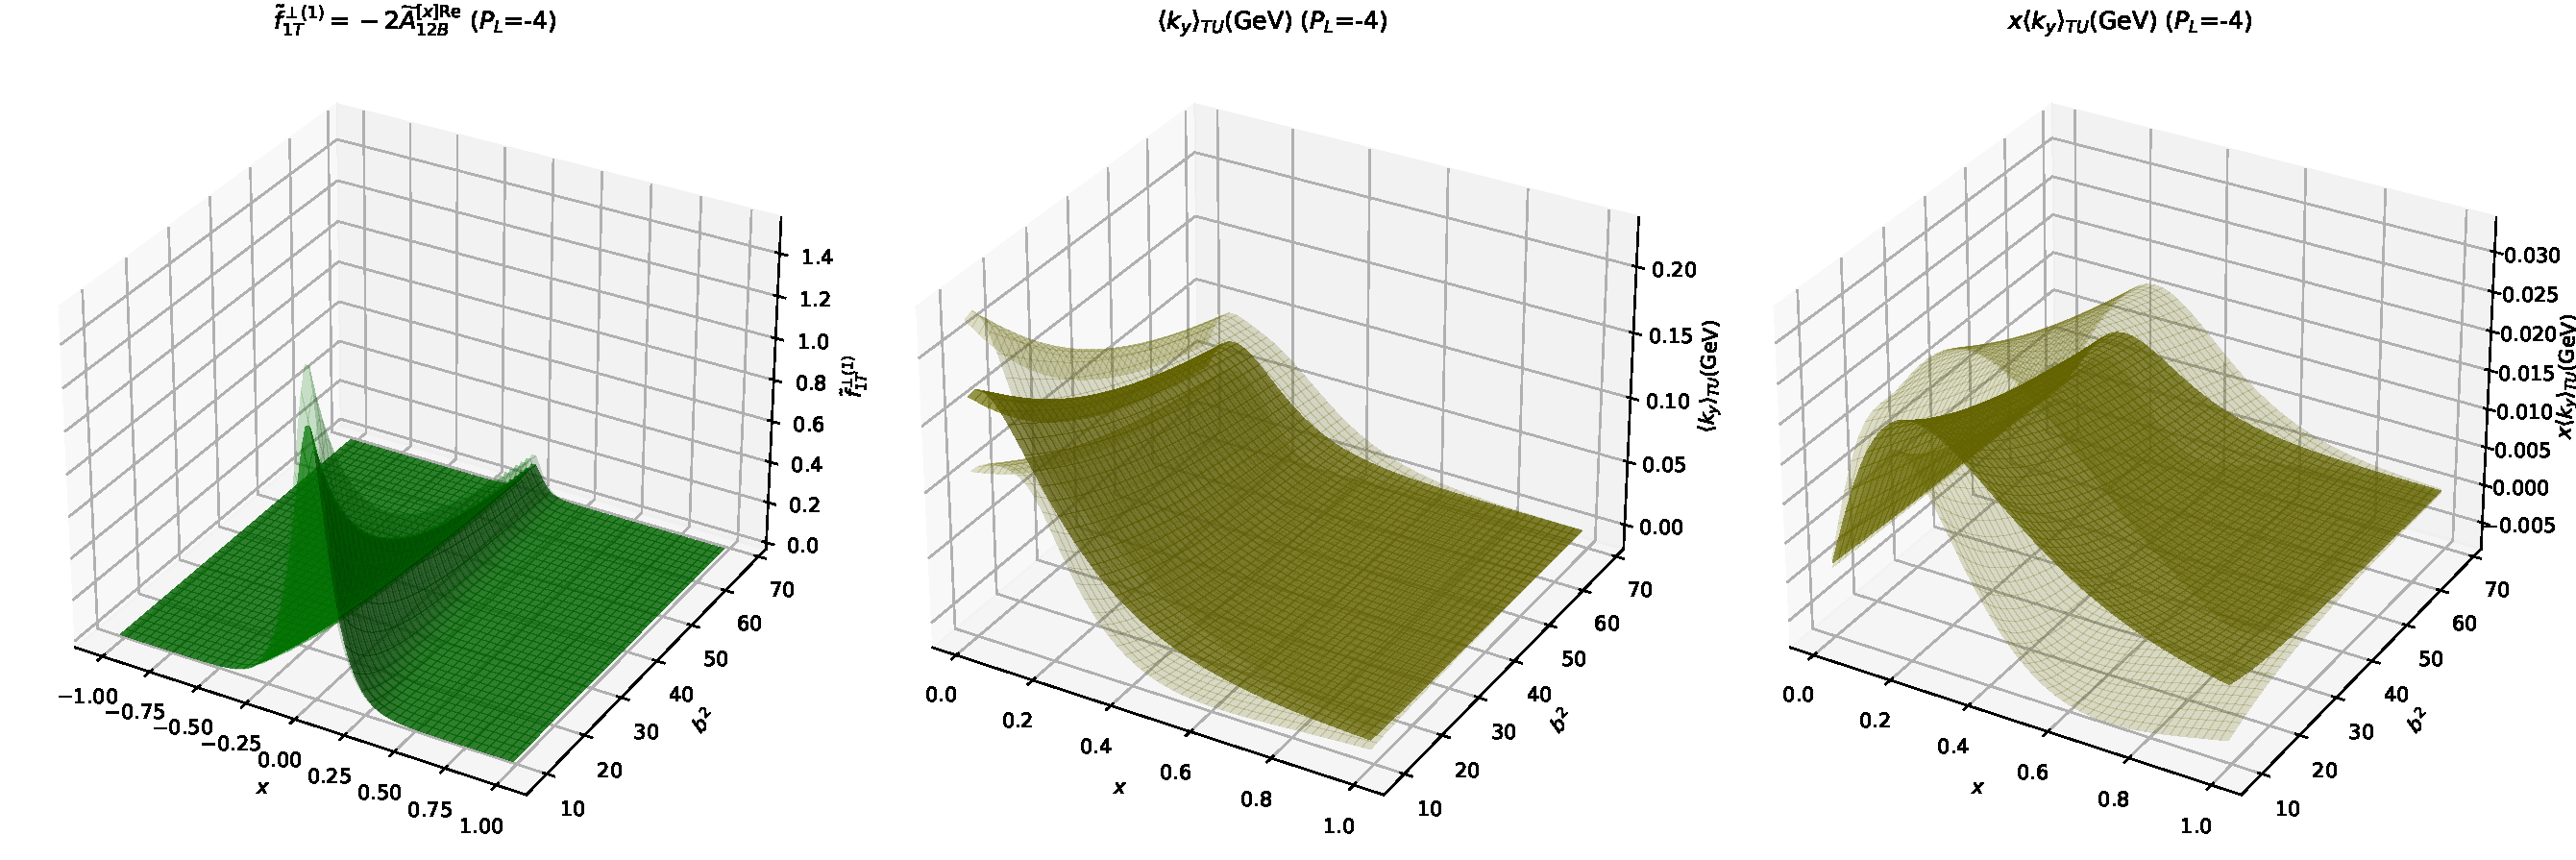
\includegraphics[width=\linewidth,height=.70\textheight,keepaspectratio]{fitting/FT_xdep_3D_A2B_A12B_bmin3_eta610_PL-4__row2.pdf}
\par\small Sivers transform, shift, and $x\langle k_y\rangle_{TU}$. Full $b^2/a^2\in[9,68]$ dependence.

\figsrc{Thesis: SimultaneousFitsCov; FT\_xdep\_3D\_A2B\_A12B\_bmin3\_eta610\_PL-4}
\end{frame}

\begin{frame}{Separable simultaneous candidate: ExpPb / Expb}
\begin{align*}
\tAmp_{2B}^{\mathrm{Re}}&=a_Re^{-c_R|\nu|}e^{-d_R\sqrt{b^2}}e^{-f\eta}\\[4mm]
\tAmp_{2B}^{\mathrm{Im}}&=a_I\nu e^{-c_I|\nu|}e^{-d_I\sqrt{b^2}}e^{-f\eta}\\[4mm]
\tAmp_{12B}^{\mathrm{Re}}&=-a_Se^{-c_S|\nu|}e^{-d_S\sqrt{b^2}}e^{-f\eta}\\[4mm]
\end{align*} Shared $f$; the spatial coefficients are fitted separately for $R,I,S$. All fits retain the same cut and staple interval.
\figsrc{Thesis: Fitting Methodologies and Stability Analysis}
\end{frame}

\begin{frame}{Separable simultaneous candidate: ExpPb / PowerLawb}
\begin{align*}
\tAmp_{2B}^{\mathrm{Re}}&=a_Re^{-c_R|\nu|}(1+d_Rb^2)^{-j_R}e^{-f\eta}\\[4mm]
\tAmp_{2B}^{\mathrm{Im}}&=a_I\nu e^{-c_I|\nu|}(1+d_Ib^2)^{-j_I}e^{-f\eta}\\[4mm]
\tAmp_{12B}^{\mathrm{Re}}&=-a_Se^{-c_S|\nu|}(1+d_Sb^2)^{-j_S}e^{-f\eta}\\[4mm]
\end{align*} Shared $f$; the spatial coefficients are fitted separately for $R,I,S$. All fits retain the same cut and staple interval.
\figsrc{Thesis: Fitting Methodologies and Stability Analysis}
\end{frame}

\begin{frame}{Separable simultaneous candidate: GaussianPb / Expb}
\begin{align*}
\tAmp_{2B}^{\mathrm{Re}}&=a_Re^{-c_R\nu^2}e^{-d_R\sqrt{b^2}}e^{-f\eta}\\[4mm]
\tAmp_{2B}^{\mathrm{Im}}&=a_I\nu e^{-c_I\nu^2}e^{-d_I\sqrt{b^2}}e^{-f\eta}\\[4mm]
\tAmp_{12B}^{\mathrm{Re}}&=-a_Se^{-c_S\nu^2}e^{-d_S\sqrt{b^2}}e^{-f\eta}\\[4mm]
\end{align*} Shared $f$; the spatial coefficients are fitted separately for $R,I,S$. All fits retain the same cut and staple interval.
\figsrc{Thesis: Fitting Methodologies and Stability Analysis}
\end{frame}

\begin{frame}{Separable simultaneous candidate: GaussianPb / PowerLawb}
\begin{align*}
\tAmp_{2B}^{\mathrm{Re}}&=a_Re^{-c_R\nu^2}(1+d_Rb^2)^{-j_R}e^{-f\eta}\\[4mm]
\tAmp_{2B}^{\mathrm{Im}}&=a_I\nu e^{-c_I\nu^2}(1+d_Ib^2)^{-j_I}e^{-f\eta}\\[4mm]
\tAmp_{12B}^{\mathrm{Re}}&=-a_Se^{-c_S\nu^2}(1+d_Sb^2)^{-j_S}e^{-f\eta}\\[4mm]
\end{align*} Shared $f$; the spatial coefficients are fitted separately for $R,I,S$. All fits retain the same cut and staple interval.
\figsrc{Thesis: Fitting Methodologies and Stability Analysis}
\end{frame}

\begin{frame}{Separable candidates: fit quality at every momentum}

\small\renewcommand{\arraystretch}{1.6}\begin{tabular}{lcccc}\toprule
Model & $P_L=-1$ & $P_L=-2$ & $P_L=-3$ & $P_L=-4$\\\midrule
ExpPb / Expb & $1.406(92)$ & $0.956(75)$ & $0.622(61)$ & $0.455(53)$\\
ExpPb / PowerLawb & $1.286(89)$ & $0.938(75)$ & $0.623(61)$ & $0.447(53)$\\
GaussianPb / Expb & $2.389(121)$ & $2.005(111)$ & $0.945(76)$ & $0.453(52)$\\
GaussianPb / PowerLawb & $2.316(120)$ & $1.981(111)$ & $0.948(76)$ & $0.448(52)$\\
Coupled power law & $1.85(10)$ & $1.197(85)$ & $0.712(66)$ & $0.434(51)$\\\bottomrule
\end{tabular}\par\medskip Entries reproduce the thesis-reported $\chi^2/\mathrm{dof}$. The coupled fit uses the augmented objective with priors; raw values alone do not establish a model preference.
\figsrc{Thesis: Fitting Methodologies and Stability Analysis}
\end{frame}

\begin{frame}{Separable candidates: width and sign diagnostics}

\small\renewcommand{\arraystretch}{1.5}\begin{tabular}{lccc}\toprule
Model at $P_L=-1$ & $c_I$ & $c_S$ & $a_I$\\\midrule
ExpPb / Expb & $0.0010(262)$ & $0.045(23)$ & $-0.167(16)$\\
ExpPb / PowerLawb & $0.0045(248)$ & $0.028(24)$ & $-0.167(31)$\\
GaussianPb / Expb & $0.568(171)$ & $0.0038(69)$ & $+0.050(121)$\\
GaussianPb / PowerLawb & $0.602(48)$ & $0.0016(61)$ & $+0.168(92)$\\
Coupled power law & $0.2253(69)$ & $0.0773(46)$ & $+0.267(13)$\\\bottomrule
\end{tabular}
\begin{itemize}
\item Several separable widths are statistically compatible with zero: longitudinal decay is weakly constrained. At $c=0$ it is lost; at $c<0$ the continuation grows.
\item Negative fitted $a_I$ is a sign mismatch with the selected convention, not a general prohibition on signed amplitudes.
\item For $c>0$, $e^{-c|\nu|}$ has a first-derivative cusp; $\nu e^{-c|\nu|}$ has a continuous first derivative but a discontinuous second derivative. Odd parity alone does not exclude it.
\end{itemize}
\figsrc{Thesis: Fitting Methodologies and Stability Analysis}
\end{frame}

\begin{frame}{What survives the complete model comparison}

\begin{itemize}
\item The chosen power law couples $\nu^2$ and $b^2$ in one denominator and supports the required Fourier continuation under explicit positivity and exponent conditions.
\item The three-amplitude fit, not the real unpolarized channel alone, constrains the Sivers shift.
\item All four momenta have now been inspected in spatial coordinates, invariant coordinates, $x$ space, and integrated observables.
\item The next step extrapolates the resulting shift in $\hat\zeta$ while carrying the model and statistical limitations forward.
\end{itemize}
\figsrc{Thesis: Fitting Methodologies and Stability Analysis}
\end{frame}
